% Options for packages loaded elsewhere
\PassOptionsToPackage{unicode}{hyperref}
\PassOptionsToPackage{hyphens}{url}
\PassOptionsToPackage{dvipsnames,svgnames,x11names}{xcolor}
%
\documentclass[
  a4paper,
]{book}

\usepackage{amsmath,amssymb}
\usepackage{iftex}
\ifPDFTeX
  \usepackage[T1]{fontenc}
  \usepackage[utf8]{inputenc}
  \usepackage{textcomp} % provide euro and other symbols
\else % if luatex or xetex
  \usepackage{unicode-math}
  \defaultfontfeatures{Scale=MatchLowercase}
  \defaultfontfeatures[\rmfamily]{Ligatures=TeX,Scale=1}
\fi
\usepackage{lmodern}
\ifPDFTeX\else  
    % xetex/luatex font selection
\fi
% Use upquote if available, for straight quotes in verbatim environments
\IfFileExists{upquote.sty}{\usepackage{upquote}}{}
\IfFileExists{microtype.sty}{% use microtype if available
  \usepackage[]{microtype}
  \UseMicrotypeSet[protrusion]{basicmath} % disable protrusion for tt fonts
}{}
\makeatletter
\@ifundefined{KOMAClassName}{% if non-KOMA class
  \IfFileExists{parskip.sty}{%
    \usepackage{parskip}
  }{% else
    \setlength{\parindent}{0pt}
    \setlength{\parskip}{6pt plus 2pt minus 1pt}}
}{% if KOMA class
  \KOMAoptions{parskip=half}}
\makeatother
\usepackage{xcolor}
\usepackage[paperwidth=8.0000000000000in,paperheight=10.000000000000in,left=1.25in,textwidth=
5.25in,top=1.00in,textheight=8.25in]{geometry}
\setlength{\emergencystretch}{3em} % prevent overfull lines
\setcounter{secnumdepth}{5}
% Make \paragraph and \subparagraph free-standing
\ifx\paragraph\undefined\else
  \let\oldparagraph\paragraph
  \renewcommand{\paragraph}[1]{\oldparagraph{#1}\mbox{}}
\fi
\ifx\subparagraph\undefined\else
  \let\oldsubparagraph\subparagraph
  \renewcommand{\subparagraph}[1]{\oldsubparagraph{#1}\mbox{}}
\fi


\providecommand{\tightlist}{%
  \setlength{\itemsep}{0pt}\setlength{\parskip}{0pt}}\usepackage{longtable,booktabs,array}
\usepackage{calc} % for calculating minipage widths
% Correct order of tables after \paragraph or \subparagraph
\usepackage{etoolbox}
\makeatletter
\patchcmd\longtable{\par}{\if@noskipsec\mbox{}\fi\par}{}{}
\makeatother
% Allow footnotes in longtable head/foot
\IfFileExists{footnotehyper.sty}{\usepackage{footnotehyper}}{\usepackage{footnote}}
\makesavenoteenv{longtable}
\usepackage{graphicx}
\makeatletter
\def\maxwidth{\ifdim\Gin@nat@width>\linewidth\linewidth\else\Gin@nat@width\fi}
\def\maxheight{\ifdim\Gin@nat@height>\textheight\textheight\else\Gin@nat@height\fi}
\makeatother
% Scale images if necessary, so that they will not overflow the page
% margins by default, and it is still possible to overwrite the defaults
% using explicit options in \includegraphics[width, height, ...]{}
\setkeys{Gin}{width=\maxwidth,height=\maxheight,keepaspectratio}
% Set default figure placement to htbp
\makeatletter
\def\fps@figure{htbp}
\makeatother
\newlength{\cslhangindent}
\setlength{\cslhangindent}{1.5em}
\newlength{\csllabelwidth}
\setlength{\csllabelwidth}{3em}
\newlength{\cslentryspacingunit} % times entry-spacing
\setlength{\cslentryspacingunit}{\parskip}
\newenvironment{CSLReferences}[2] % #1 hanging-ident, #2 entry spacing
 {% don't indent paragraphs
  \setlength{\parindent}{0pt}
  % turn on hanging indent if param 1 is 1
  \ifodd #1
  \let\oldpar\par
  \def\par{\hangindent=\cslhangindent\oldpar}
  \fi
  % set entry spacing
  \setlength{\parskip}{#2\cslentryspacingunit}
 }%
 {}
\usepackage{calc}
\newcommand{\CSLBlock}[1]{#1\hfill\break}
\newcommand{\CSLLeftMargin}[1]{\parbox[t]{\csllabelwidth}{#1}}
\newcommand{\CSLRightInline}[1]{\parbox[t]{\linewidth - \csllabelwidth}{#1}\break}
\newcommand{\CSLIndent}[1]{\hspace{\cslhangindent}#1}

\usepackage{makeidx}
\usepackage{pdfpages}

%reduce vertical spacing in toc - not needed once tocloft added below
%\usepackage{etoolbox}
%\makeatletter
%  \pretocmd{\chapter}{\addtocontents{toc}{\protect\addvspace{-1\p@}}}{}{}
%  \pretocmd{\section}{\addtocontents{toc}{\protect\addvspace{-5\p@}}}{}{}
%\pretocmd{\subsection}{\addtocontents{toc}{\protect\addvspace{-5\p@}}}{}{}
%\makeatother

%\makeatletter
%  \providecommand*\setfloatlocations[2]{\@namedef{fps@#1}{#2}}
%\makeatother
%\setfloatlocations{figure}{htbp}
%\setfloatlocations{table}{htbp}

\usepackage{titling}
\let\oldmaketitle\maketitle

\usepackage{atbegshi}% http://ctan.org/pkg/atbegshi
\AtBeginDocument{\let\maketitle\relax}
\AtBeginDocument{\AtBeginShipoutNext{\AtBeginShipoutDiscard}} % Discard next blank page

\usepackage{tocloft}
\cftsetindents{section}{2em}{2.5em}
\cftsetindents{subsection}{5em}{3em}

\usepackage{enotez}
\DeclareInstance{enotez-list}{section}{paragraph}{heading=\chapter}
\setenotez{split=chapter,backref=true,list-name=Chapter notes,totoc=chapter}

%define command for adding footnote textbox to first page of each chapter
\newcommand{\placetextbox}[3]{% \placetextbox{<horizontal pos>}{<vertical pos>}{<stuff>}
  \setbox0=\hbox{#3}% Put <stuff> in a box
  \AddToShipoutPictureFG*{% Add <stuff> to current page foreground
    \put(\LenToUnit{#1\paperwidth},\LenToUnit{#2\paperheight}){\vtop{{\null}\makebox[0pt][c]{#3}}}%
  }%
}%

\newcommand{\quotes}[1]{``#1''}

\usepackage{array}
\usepackage{caption}
\usepackage{graphicx}
\usepackage{siunitx}
\usepackage[normalem]{ulem}
\usepackage{colortbl}
\usepackage{multirow}
\usepackage{hhline}
\usepackage{calc}
\usepackage{tabularx}
\usepackage{threeparttable}
\usepackage{wrapfig}
\usepackage{adjustbox}
\usepackage{hyperref}
\makeatletter
\makeatother
\makeatletter
\@ifpackageloaded{bookmark}{}{\usepackage{bookmark}}
\makeatother
\makeatletter
\@ifpackageloaded{caption}{}{\usepackage{caption}}
\AtBeginDocument{%
\ifdefined\contentsname
  \renewcommand*\contentsname{Table of contents}
\else
  \newcommand\contentsname{Table of contents}
\fi
\ifdefined\listfigurename
  \renewcommand*\listfigurename{List of Figures}
\else
  \newcommand\listfigurename{List of Figures}
\fi
\ifdefined\listtablename
  \renewcommand*\listtablename{List of Tables}
\else
  \newcommand\listtablename{List of Tables}
\fi
\ifdefined\figurename
  \renewcommand*\figurename{Figure}
\else
  \newcommand\figurename{Figure}
\fi
\ifdefined\tablename
  \renewcommand*\tablename{Table}
\else
  \newcommand\tablename{Table}
\fi
}
\@ifpackageloaded{float}{}{\usepackage{float}}
\floatstyle{ruled}
\@ifundefined{c@chapter}{\newfloat{codelisting}{h}{lop}}{\newfloat{codelisting}{h}{lop}[chapter]}
\floatname{codelisting}{Listing}
\newcommand*\listoflistings{\listof{codelisting}{List of Listings}}
\makeatother
\makeatletter
\@ifpackageloaded{caption}{}{\usepackage{caption}}
\@ifpackageloaded{subcaption}{}{\usepackage{subcaption}}
\makeatother
\makeatletter
\@ifpackageloaded{tcolorbox}{}{\usepackage[skins,breakable]{tcolorbox}}
\makeatother
\makeatletter
\@ifundefined{shadecolor}{\definecolor{shadecolor}{rgb}{.97, .97, .97}}
\makeatother
\makeatletter
\makeatother
\makeatletter
\makeatother
\ifLuaTeX
  \usepackage{selnolig}  % disable illegal ligatures
\fi
\IfFileExists{bookmark.sty}{\usepackage{bookmark}}{\usepackage{hyperref}}
\IfFileExists{xurl.sty}{\usepackage{xurl}}{} % add URL line breaks if available
\urlstyle{same} % disable monospaced font for URLs
\hypersetup{
  pdftitle={LEARNING STATISTICS WITH JAMOVI},
  colorlinks=true,
  linkcolor={Maroon},
  filecolor={Maroon},
  citecolor={Blue},
  urlcolor={Blue},
  pdfcreator={LaTeX via pandoc}}

\title{LEARNING STATISTICS WITH JAMOVI}
\author{}
\date{}

\begin{document}
\frontmatter
\maketitle
\begin{center}
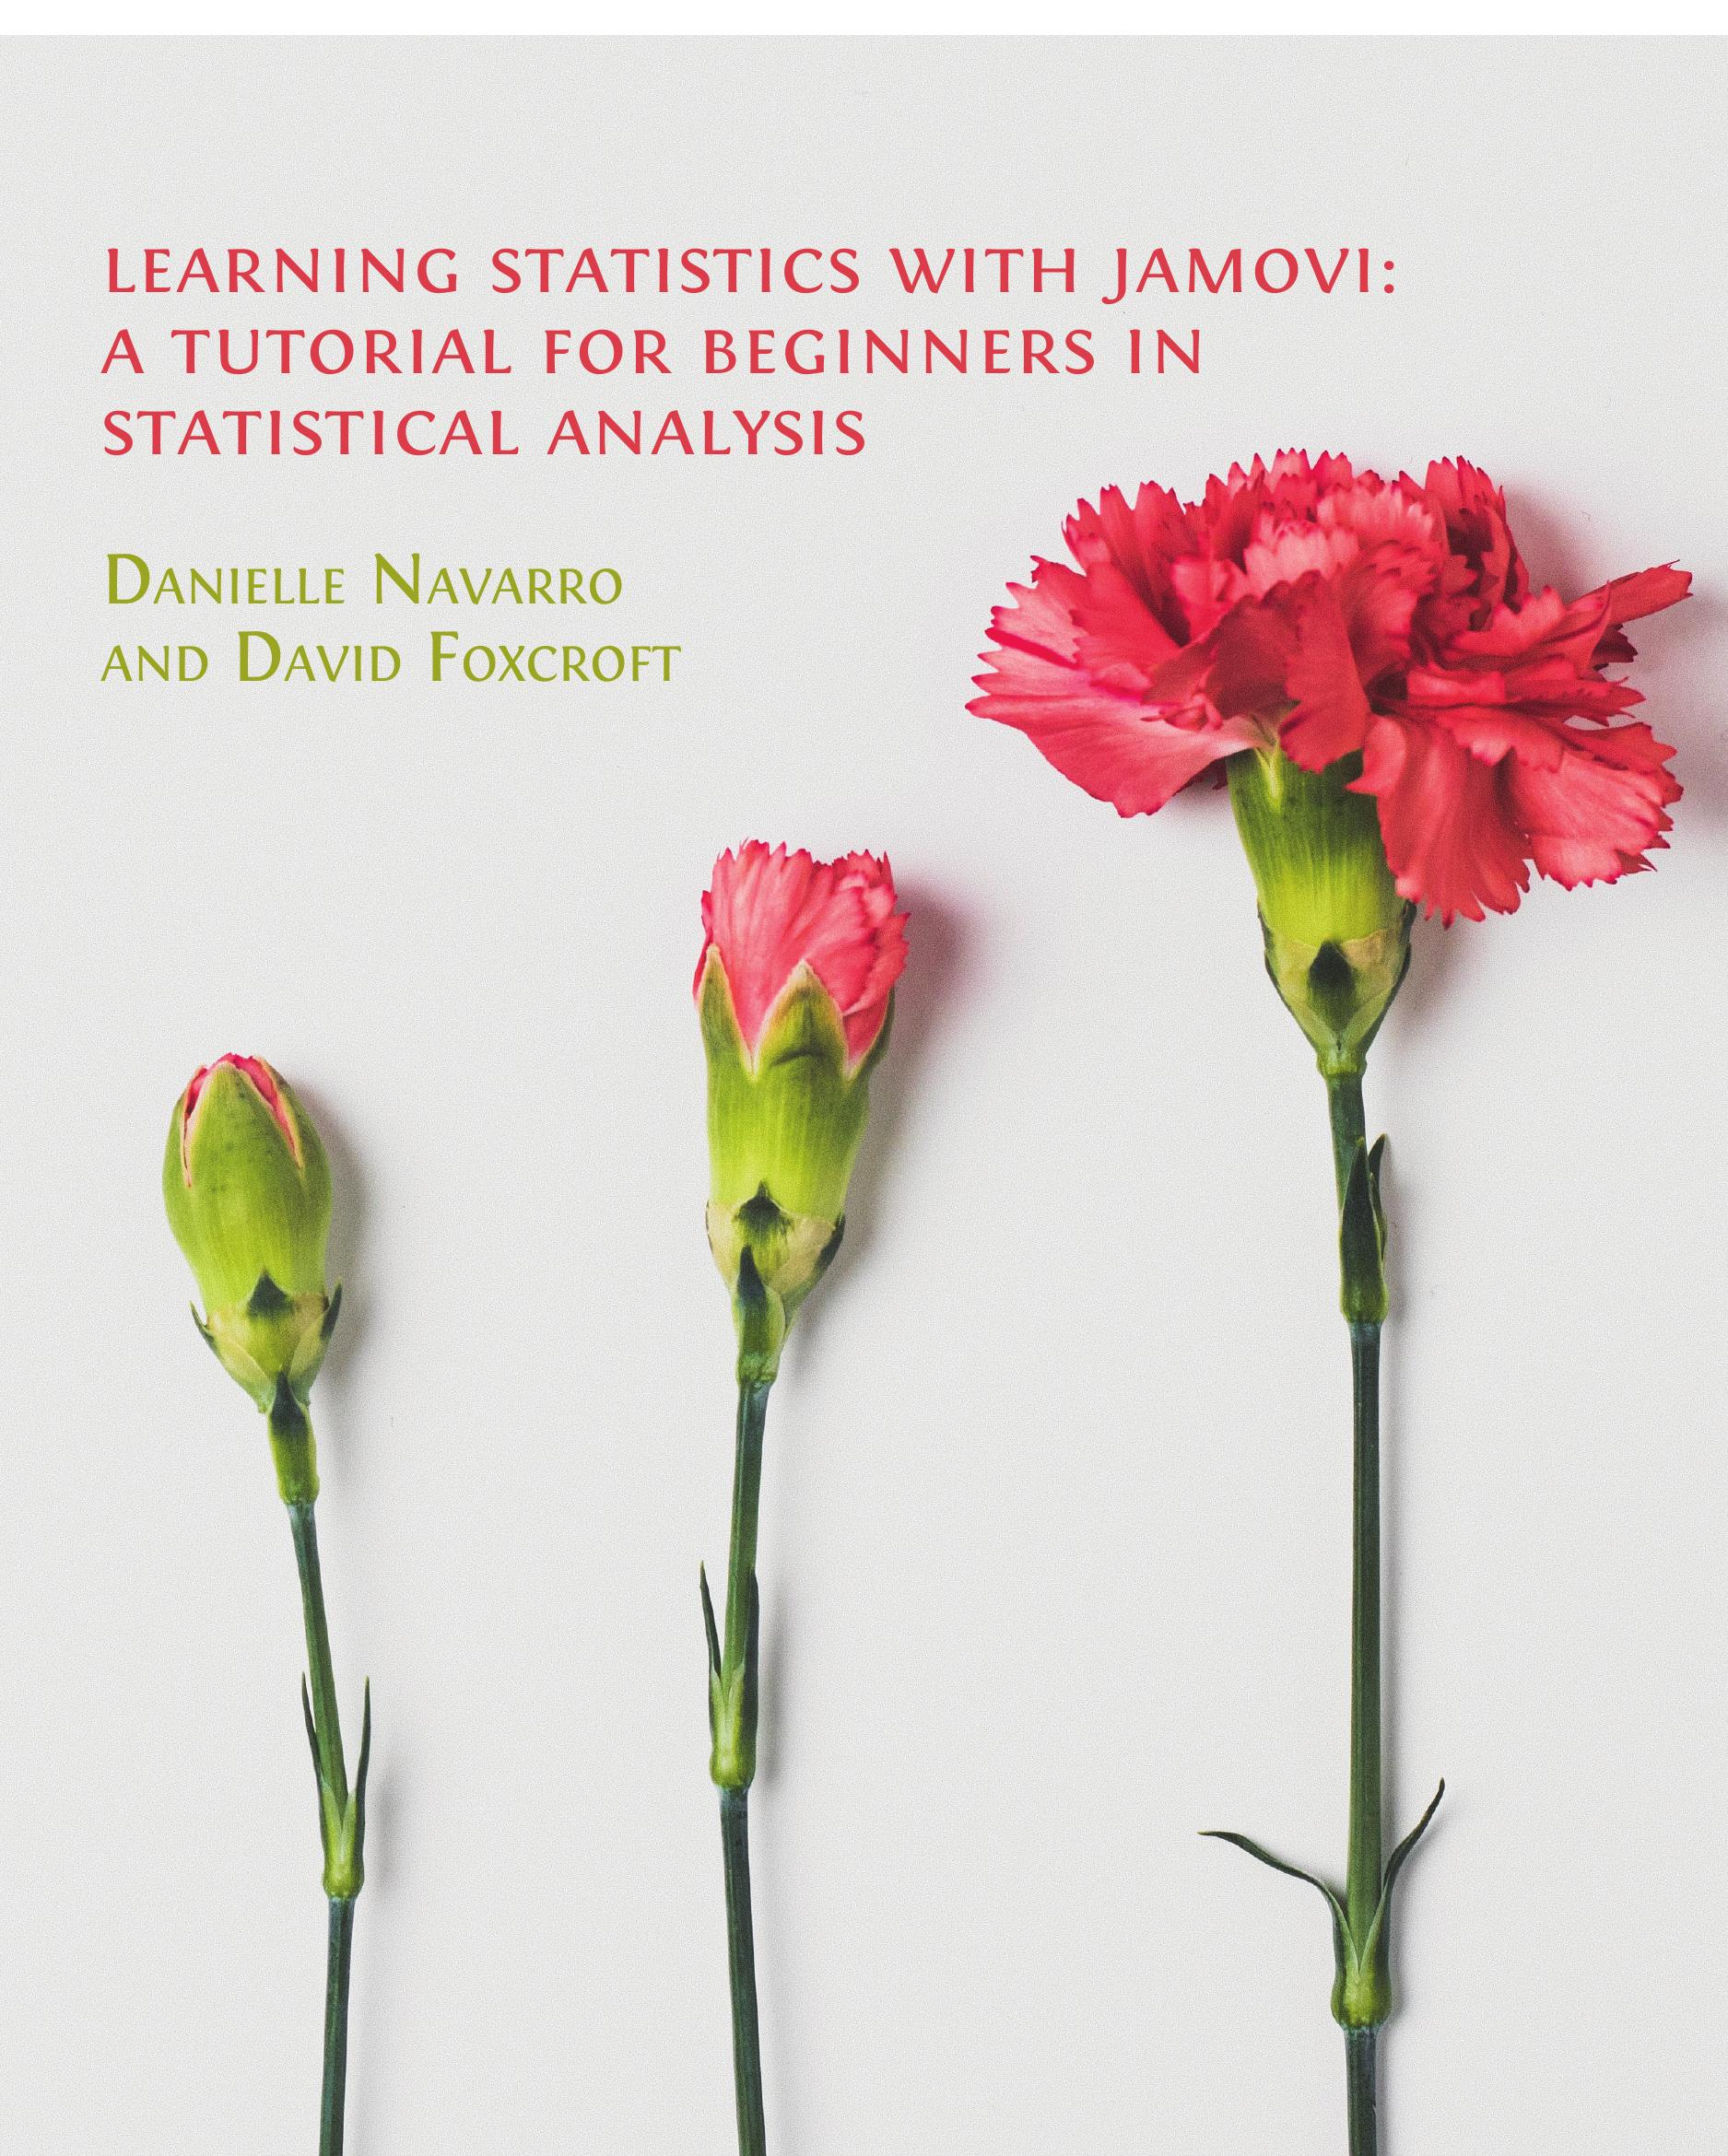
\includepdf[fitpaper=true,pages=-]{images/obp.0333}
\end{center}
\pagestyle{empty}

\let\maketitle\oldmaketitle
\maketitle

\mainmatter
\pagestyle{plain}

\let\footnote=\endnote



\pagenumbering{roman}
\hspace{0pt}
\vfill
\begin{center}

\Huge{Learning Statistics with jamovi}

\Large{A Tutorial for Beginners in Statistical Analysis}\\*[20pt]

\normalsize{Danielle Navarro and David Foxcroft}

\vfill
\end{center}
\hspace{0pt}
\pagebreak

\hspace{0pt}
\vfill

\copyright 2025 David Foxcroft and Danielle Navarro

This work is licensed under an Attribution-ShareAlike 4.0 International (CC BY-SA 4.0).

This license allows you to copy and redistribute, transform, and build upon the material for any purpose, even commercially. providing attribution is made to the authors (but not in any way that suggests that they endorse you or your use of the work). Attribution should include the following information:

Danielle Navarro and David Foxcroft, \textit{Learning statistics with jamovi: A tutorial for beginners in statistical analysis}. Cambridge, UK: Open Book Publishers, 2025, \url{https://doi.org/10.11647/OBP.0333}

Further details about CC BY-SA licenses are available at \\ \url{https://creativecommons.org/licenses/by-sa/4.0/}

All external links were active at the time of publication unless otherwise stated and have been archived via the Internet Archive Wayback Machine at \\ \url{https://archive.org/web}

Digital material and resources associated with this volume are available at \\ \url{https://doi.org/10.11647/OBP.0333\#resources}

ISBN Paperback: 978-1-80064-937-8

ISBN Hardback: 978-1-80064-938-5

ISBN Digital (PDF): 978-1-80064-939-2

DOI: 10.11647/OBP.0333


\vfill
\hspace{0pt}
\pagebreak

\hspace{0pt}
\vfill

This textbook covers the contents of an introductory statistics class, as typically taught to undergraduate psychology, health or social science students. The book covers how to get started in jamovi as well as giving an introduction to data manipulation. From a statistical perspective, the book discusses descriptive statistics and graphing first, followed by chapters on probability theory, sampling and estimation, and null hypothesis testing. After introducing the theory, the book covers the analysis of contingency tables, correlation, \textit{t}-tests, regression, ANOVA and factor analysis. Bayesian statistics are touched on at the end of the book.

Data sets used in the book are freely available for use in jamovi. All the data files you need can be accessed within jamovi via an add-on module in the jamovi library. Or you can download the files from \url{https://www.learnstatswithjamovi.com}.


Citation: Danielle Navarro and David Foxcroft, \textit{Learning statistics with jamovi: A tutorial for beginners in statistical analysis}. Cambridge, UK: Open Book Publishers, 2025, \url{https://doi.org/10.11647/OBP.0333}

\vfill
\hspace{0pt}

\ifdefined\Shaded\renewenvironment{Shaded}{\begin{tcolorbox}[frame hidden, sharp corners, interior hidden, boxrule=0pt, enhanced, borderline west={3pt}{0pt}{shadecolor}, breakable]}{\end{tcolorbox}}\fi

\renewcommand*\contentsname{Table of contents}
{
\hypersetup{linkcolor=}
\setcounter{tocdepth}{2}
\tableofcontents
}
\mainmatter
\bookmarksetup{startatroot}

\hypertarget{preface}{%
\chapter*{Preface}\label{preface}}
\addcontentsline{toc}{chapter}{Preface}

\markboth{Preface}{Preface}

This book is an adaptation of DJ Navarro (2018). Learning statistics
with R: A tutorial for psychology students and other beginners. (Version
0.6). \url{https://learningstatisticswithr.com/}.

The jamovi version of this book was first released in 2018, as version
0.65. Versions 0.70 and 0.75 were released in subsequent years with
corrections and additions; details of the changes in earlier versions of
the book can be found in the preface to version 0.75:
\url{https://github.com/user-attachments/files/18124061/learning-statistics-with-jamovi-0.75.pdf}.
In that time, many people have contacted us asking for a hard copy
version of the book. To achieve this, and to preserve the open source
attributes of the book and materials, we have worked with
\href{https://www.openbookpublishers.com/books/10.11647/obp.0333}{Open
Book Publishers} in Cambridge, UK, to release this updated version. Open
Book Publishers are the leading independent open access publisher of
academic research in the Humanities and Social Sciences in the UK. They
are award-winning, not-for-profit, run by scholars, and committed to
making high-quality research freely available to readers around the
world.

If you spot any mistakes, of have any suggestions, please do let us know
by raising an issue at
\url{https://github.com/davidfoxcroft/lsj-book/issues}.

\emph{David Foxcroft\\
January 1st, 2025}

\part{Statistical tools}

\hypertarget{sec-Comparing-several-means-one-way-ANOVA}{%
\chapter{Comparing several means (one-way
ANOVA)}\label{sec-Comparing-several-means-one-way-ANOVA}}

\placetextbox{0.26}{0.06}{\scriptsize{©2025 D. Foxcroft and D. Navarro,}}
\placetextbox{0.20}{0.05}{\scriptsize{CC BY-NC 4.0}}
\placetextbox{0.70}{0.06}{\scriptsize{\url{https://doi.org/10.11647/OBP.0333/13}}}

This chapter introduces one of the most widely used tools in
psychological statistics, known as ``the analysis of variance'', but
usually referred to as ANOVA. The basic technique was developed by Sir
Ronald Fisher in the early 20th century and it is to him that we owe the
rather unfortunate terminology. The term ANOVA is a little misleading,
in two respects. Firstly, although the name of the technique refers to
variances, ANOVA is concerned with investigating differences in means.
Secondly, there are several different things out there that are all
referred to as ANOVAs, some of which have only a very tenuous connection
to one another. Later on in the book we'll encounter a range of
different ANOVA methods that apply in quite different situations, but
for the purposes of this chapter we'll only consider the simplest form
of ANOVA, in which we have several different groups of observations, and
we're interested in finding out whether those groups differ in terms of
some outcome variable of interest. This is the question that is
addressed by a one-way ANOVA.

The structure of this chapter is as follows: first I'll introduce a
fictitious data set that we'll use as a running example throughout the
chapter. After introducing the data, I'll describe the mechanics of how
a one-way ANOVA actually works
\protect\hyperlink{sec-How-ANOVA-works}{How ANOVA works} and then focus
on how you can run one in jamovi
\protect\hyperlink{running-an-anova-in-jamovi}{Running an ANOVA in
jamovi}. These two sections are the core of the chapter.

The remainder of the chapter discusses a range of important topics that
inevitably arise when running an ANOVA, namely how to calculate effect
sizes, post hoc tests and corrections for multiple comparisons and the
assumptions that ANOVA relies upon. We'll also talk about how to check
those assumptions and some of the things you can do if the assumptions
are violated. Then we'll cover repeated measures ANOVA.

\hypertarget{an-illustrative-data-set}{%
\section{An illustrative data set}\label{an-illustrative-data-set}}

Suppose you've become involved in a clinical trial in which you are
testing a new antidepressant drug called \emph{Joyzepam}. In order to
construct a fair test of the drug's effectiveness, the study involves
three separate drugs to be administered. One is a placebo, and the other
is an existing antidepressant / anti-anxiety drug called
\emph{Anxifree}. A collection of 18 participants with moderate to severe
depression are recruited for your initial testing. Because the drugs are
sometimes administered in conjunction with psychological therapy, your
study includes 9 people undergoing cognitive behavioural therapy (CBT)
and 9 who are not. Participants are randomly assigned (doubly blinded,
of course) a treatment, such that there are 3 CBT people and 3
no-therapy people assigned to each of the 3 drugs. A psychologist
assesses the mood of each person after a 3-month run with each drug, and
the overall improvement in each person's mood is assessed on a scale
ranging from \(-5\) to \(+5\). With that as the study design, let's now
load up the data file in \emph{clinicaltrial.csv} . We can see that this
data set contains the three variables drug, therapy and mood.gain.

For the purposes of this chapter, what we're really interested in is the
effect of drug on mood.gain. The first thing to do is calculate some
descriptive statistics and draw some graphs. In the
\textbf{?@sec-Descriptive-statistics} chapter we showed you how to do
this, and some of the descriptive statistics we can calculate in jamovi
are shown in Figure~\ref{fig-fig13-1}.

\begin{figure}

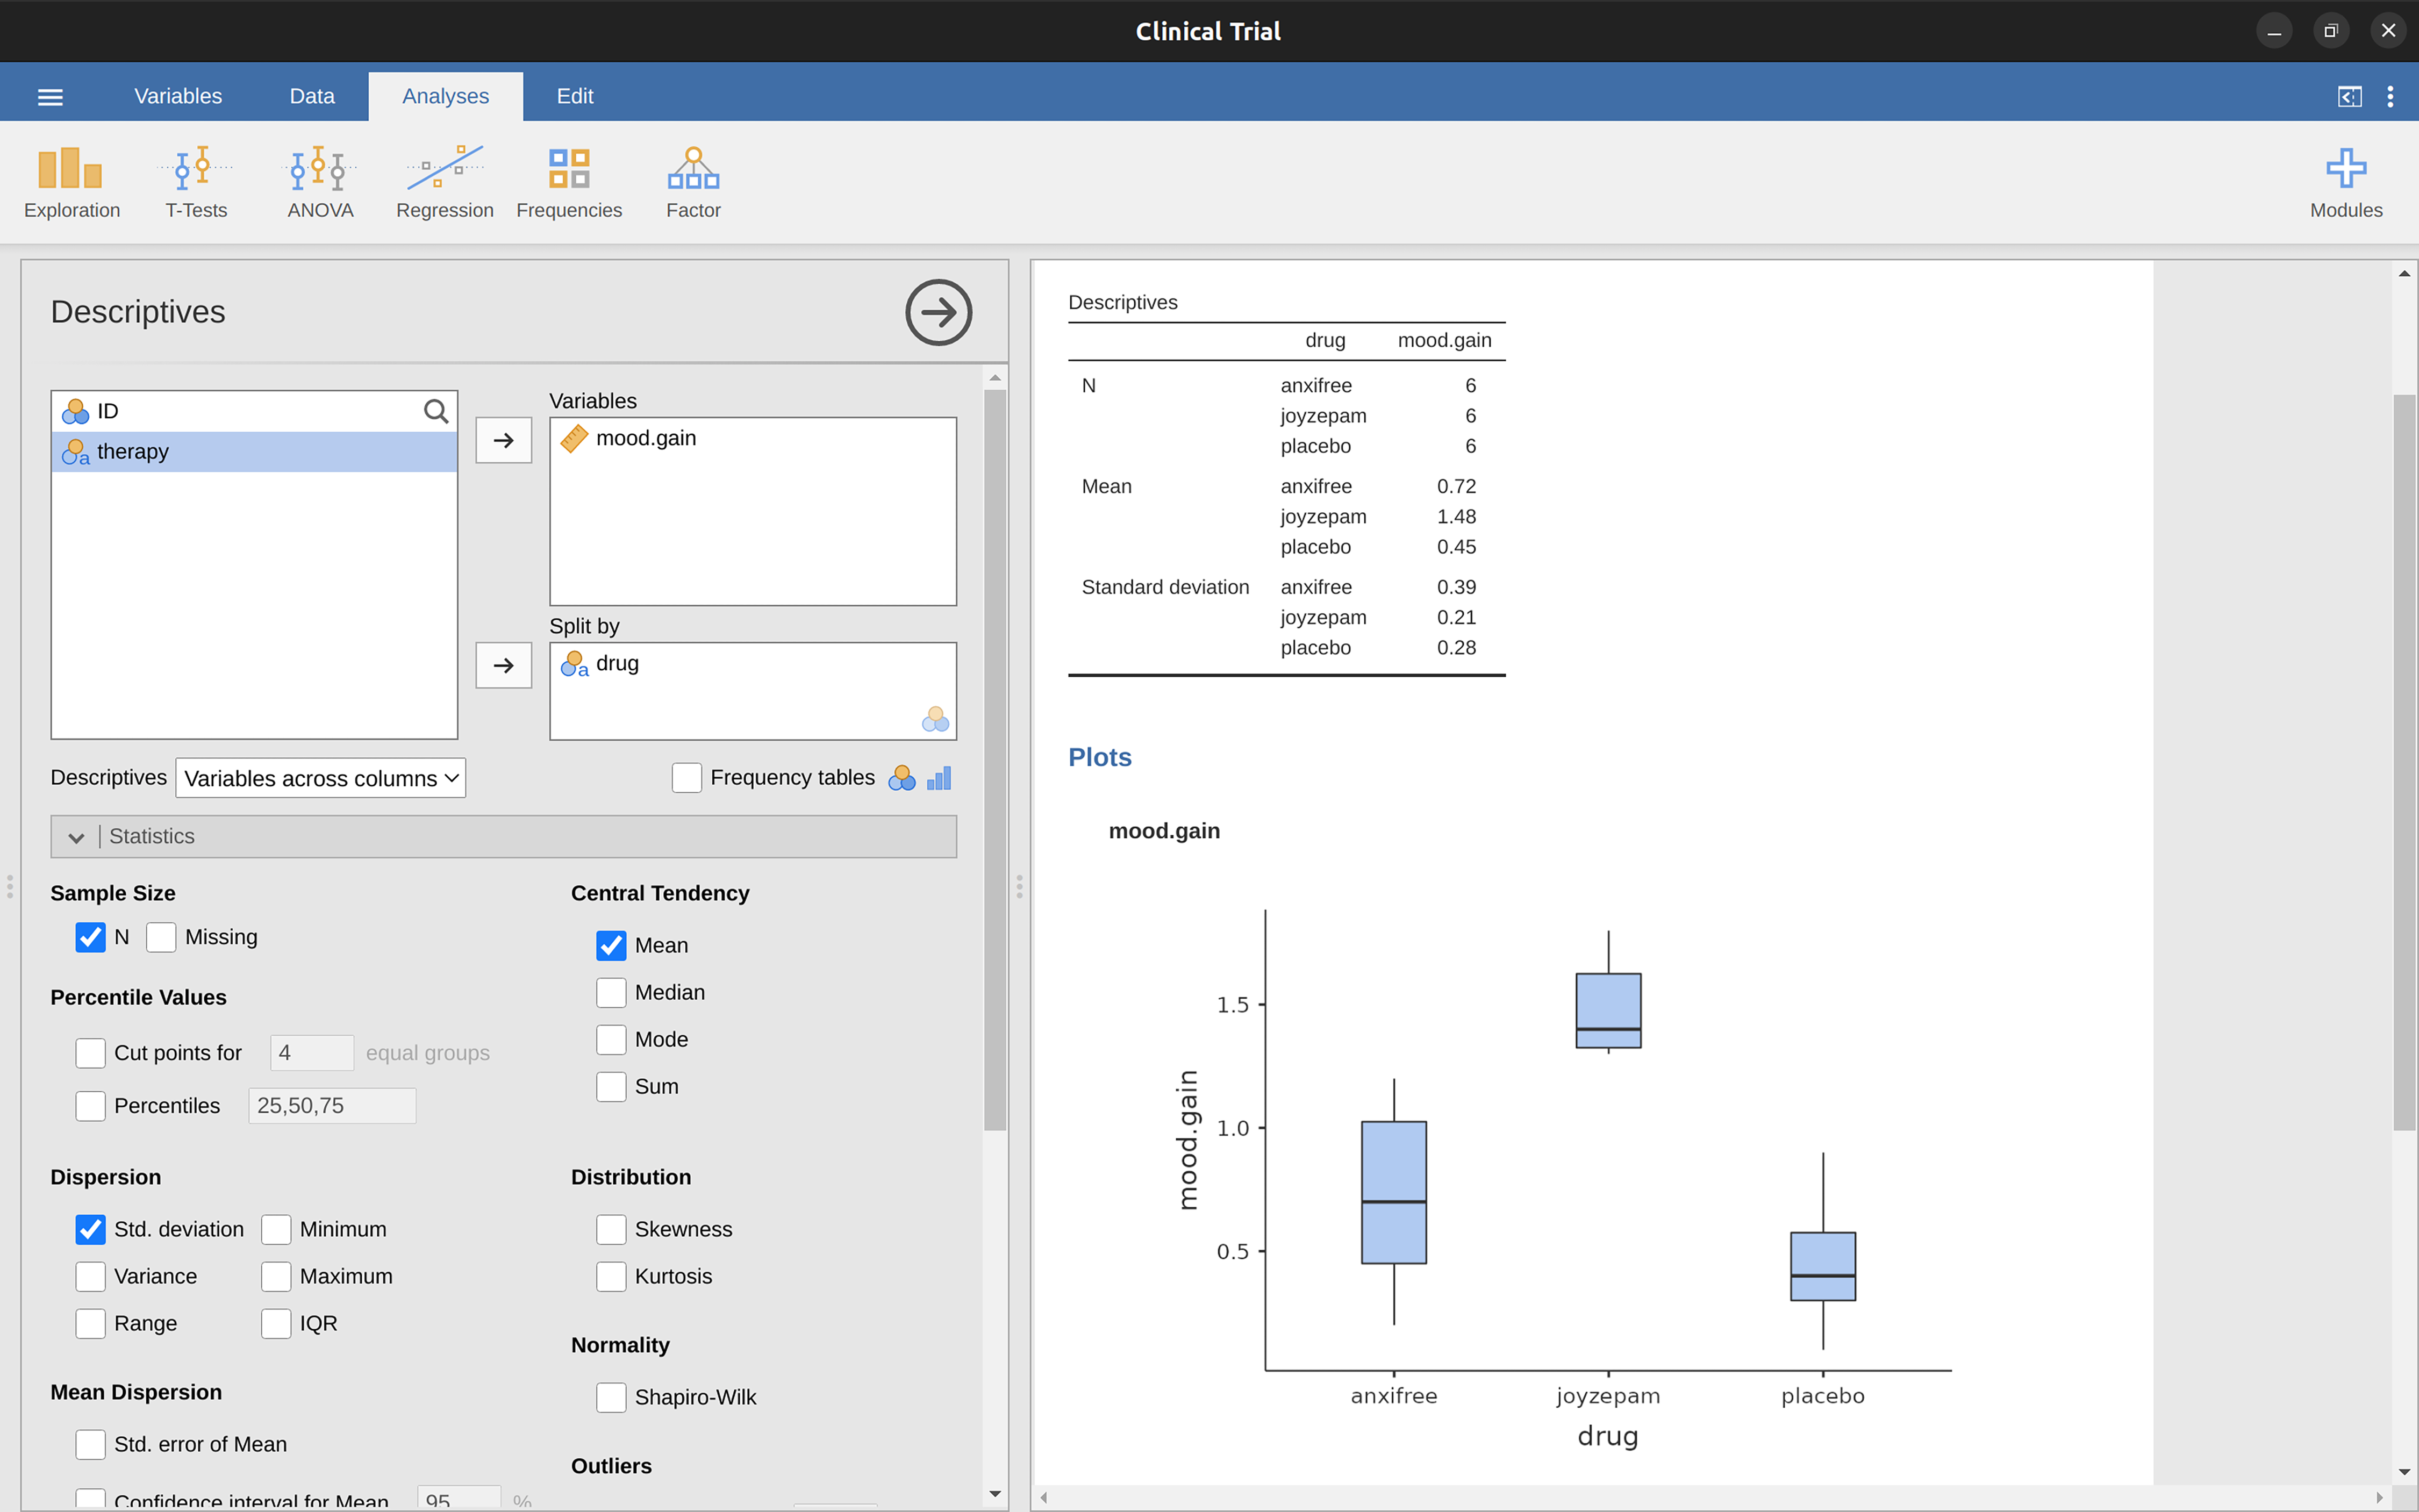
\includegraphics[width=1\textwidth,height=\textheight]{images/fig13-1.png} \hfill{}

\caption{\label{fig-fig13-1}Descriptives for mood gain, and box plots by
drug administered}

\end{figure}

As the plot makes clear, there is a larger improvement in mood for
participants in the Joyzepam group than for either the Anxifree group or
the placebo group. The Anxifree group shows a larger mood gain than the
control group, but the difference isn't as large. The question that we
want to answer is are these difference ``real'', or are they just due to
chance?

\hypertarget{sec-How-ANOVA-works}{%
\section{How ANOVA works}\label{sec-How-ANOVA-works}}

In order to answer the question posed by our clinical trial data we're
going to run a one-way ANOVA. I'm going to start by showing you how to
do it the hard way, building the statistical tool from the ground up and
showing you how you could do it if you didn't have access to any of the
cool built-in ANOVA functions in jamovi. And I hope you'll read it
carefully, try to do it the long way once or twice to make sure you
really understand how ANOVA works, and then once you've grasped the
concept never ever do it this way again.

The experimental design that I described in the previous section
strongly suggests that we're interested in comparing the average mood
change for the three different drugs. In that sense, we're talking about
an analysis similar to the \(t\)-test (see
\textbf{?@sec-Comparing-two-means}) but involving more than two groups.
If we let \(\mu_P\) denote the population mean for the mood change
induced by the placebo, and let \(\mu_A\) and \(\mu_J\) denote the
corresponding means for our two drugs, Anxifree and Joyzepam, then the
(somewhat pessimistic) null hypothesis that we want to test is that all
three population means are identical. That is, neither of the two drugs
is any more effective than a placebo. We can write out this null
hypothesis as: \[H_0: \text{ it is true that } \mu_P=\mu_A=\mu_J\] As a
consequence, our alternative hypothesis is that at least one of the
three different treatments is different from the others. It's a bit
tricky to write this mathematically, because (as we'll discuss) there
are quite a few different ways in which the null hypothesis can be
false. So for now we'll just write the alternative hypothesis like this:
\[H_1: \text{ it } \underline{ is \text{ } not } \text{ true that }
\mu_P=\mu_A=\mu_J\]

This null hypothesis is a lot trickier to test than any of the ones
we've seen previously. How shall we do it? A sensible guess would be to
``do an ANOVA'', since that's the title of the chapter, but it's not
particularly clear why an ``analysis of variances'' will help us learn
anything useful about the means. In fact, this is one of the biggest
conceptual difficulties that people have when first encountering ANOVA.
To see how this works, I find it most helpful to start by talking about
variances, specifically between group variability and within-group
variability (Figure~\ref{fig-fig13-2}).

\begin{figure}

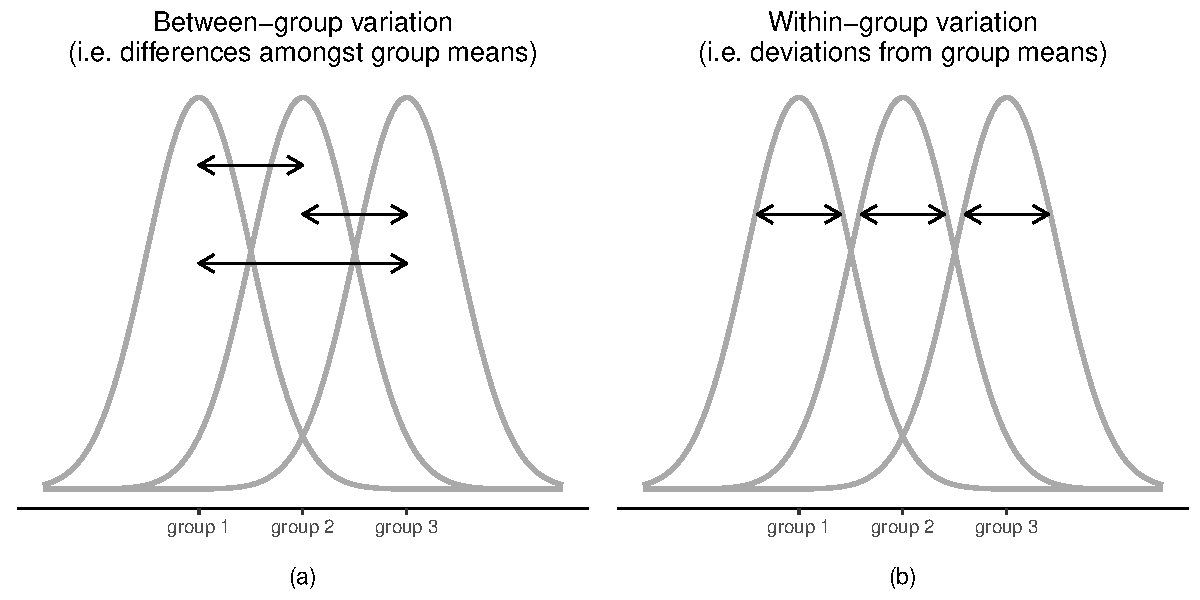
\includegraphics[width=1\textwidth,height=\textheight]{13-Comparing-several-means-one-way-ANOVA_files/figure-pdf/fig-fig13-2-1.pdf} \hfill{}

\caption{\label{fig-fig13-2}Graphical illustration of ``between groups''
variation (panel (a)) and ``within groups'' variation (panel (b)). On
the left the arrows show the differences in the group means. On the
right the arrows highlight the variability within each group}

\end{figure}

\hypertarget{two-formulas-for-the-variance-of-y}{%
\subsection{\texorpdfstring{Two formulas for the variance of
\(Y\)}{Two formulas for the variance of Y}}\label{two-formulas-for-the-variance-of-y}}

First, let's start by introducing some notation. We'll use \(G\) to
refer to the total number of groups. For our data set there are three
drugs, so there are \(G = 3\) groups. Next, we'll use \(N\) to refer to
the total sample size; there are a total of \(N = 18\) people in our
data set. Similarly, let's use \(N_k\) to denote the number of people in
the \(k\)-th group. In our fake clinical trial, the sample size is
\(N_k = 6\) for all three groups.\footnote{When all groups have the same
  number of observations, the experimental design is said to be
  ``balanced''. Balance isn't such a big deal for one-way ANOVA, which
  is the topic of this chapter. It becomes more important when you start
  doing more complicated ANOVAs.} Finally, we'll use \(Y\) to denote the
outcome variable. In our case, \(Y\) refers to mood change.
Specifically, we'll use \(Y_{ik}\) to refer to the mood change
experienced by the \(i\)-th member of the \(k\)-th group. Similarly,
we'll use \(\bar{Y}\) to be the average mood change, taken across all 18
people in the experiment, and \(\bar{Y}_k\) to refer to the average mood
change experienced by the 6 people in group \(k\).

Now that we've got our notation sorted out we can start writing down
formulas. To start with, let's recall the formula for the variance that
we used in \textbf{?@sec-Measures-of-variability}, way back in those
kinder days when we were just doing descriptive statistics. The sample
variance of \(Y\) is defined as follows:
\[Var(Y)=\frac{1}{N}\sum_{k=1}^{G}\sum_{i=1}^{N_k}(Y_{ik}-\bar{Y})^2\]
This formula looks pretty much identical to the formula for the variance
in \textbf{?@sec-Measures-of-variability}. The only difference is that
this time around I've got two summations here: I'm summing over groups
(i.e., values for \(k\)) and over the people within the groups (i.e.,
values for \(i\)). This is purely a cosmetic detail. If I'd instead used
the notation \(Y_p\) to refer to the value of the outcome variable for
person \(p\) in the sample, then I'd only have a single summation. The
only reason that we have a double summation here is that I've classified
people into groups, and then assigned numbers to people within groups.

A concrete example might be useful here. Let's consider
Table~\ref{tbl-tab13-1}, in which we have a total of \(N = 5\) people
sorted into \(G = 2\) groups. Arbitrarily, let's say that the ``cool''
people are group 1 and the ``uncool'' people are group 2. It turns out
that we have three cool people (\(N_1 = 3\)) and two uncool people
(\(N_2 = 2\)).

\hypertarget{tbl-tab13-1}{}
 
  \providecommand{\huxb}[2]{\arrayrulecolor[RGB]{#1}\global\arrayrulewidth=#2pt}
  \providecommand{\huxvb}[2]{\color[RGB]{#1}\vrule width #2pt}
  \providecommand{\huxtpad}[1]{\rule{0pt}{#1}}
  \providecommand{\huxbpad}[1]{\rule[-#1]{0pt}{#1}}

\begin{table}[ht]
\caption{\label{tbl-tab13-1}Grumpiness for people in cool and uncool groups }\tabularnewline

\begin{centerbox}
\begin{threeparttable}
\setlength{\tabcolsep}{0pt}
\begin{tabularx}{0.9\textwidth}{p{0.15\textwidth} p{0.15\textwidth} p{0.15\textwidth} p{0.15\textwidth} p{0.15\textwidth} p{0.15\textwidth}}


\hhline{>{\huxb{0, 0, 0}{0.4}}->{\huxb{0, 0, 0}{0.4}}->{\huxb{0, 0, 0}{0.4}}->{\huxb{0, 0, 0}{0.4}}->{\huxb{0, 0, 0}{0.4}}->{\huxb{0, 0, 0}{0.4}}-}
\arrayrulecolor{black}

\multicolumn{1}{!{\huxvb{0, 0, 0}{0}}p{0.15\textwidth}!{\huxvb{0, 0, 0}{0}}}{\hspace{0pt}\parbox[b]{0.15\textwidth-0pt-12pt}{\huxtpad{2pt + 1em}\centering \textbf{name}\huxbpad{2pt}}} &
\multicolumn{1}{p{0.15\textwidth}!{\huxvb{0, 0, 0}{0}}}{\hspace{12pt}\parbox[b]{0.15\textwidth-12pt-12pt}{\huxtpad{2pt + 1em}\centering \textbf{person \(P\)}\huxbpad{2pt}}} &
\multicolumn{1}{p{0.15\textwidth}!{\huxvb{0, 0, 0}{0}}}{\hspace{12pt}\parbox[b]{0.15\textwidth-12pt-12pt}{\huxtpad{2pt + 1em}\centering \textbf{group}\huxbpad{2pt}}} &
\multicolumn{1}{p{0.15\textwidth}!{\huxvb{0, 0, 0}{0}}}{\hspace{12pt}\parbox[b]{0.15\textwidth-12pt-12pt}{\huxtpad{2pt + 1em}\centering \textbf{group num. \(k\)}\huxbpad{2pt}}} &
\multicolumn{1}{p{0.15\textwidth}!{\huxvb{0, 0, 0}{0}}}{\hspace{12pt}\parbox[b]{0.15\textwidth-12pt-12pt}{\huxtpad{2pt + 1em}\centering \textbf{index in group}\huxbpad{2pt}}} &
\multicolumn{1}{p{0.15\textwidth}!{\huxvb{0, 0, 0}{0}}}{\hspace{12pt}\parbox[b]{0.15\textwidth-12pt-0pt}{\huxtpad{2pt + 1em}\centering \textbf{grumpiness \( Y_{ik} \) or \( Y_p \)}\huxbpad{2pt}}} \tabularnewline[-0.5pt]


\hhline{>{\huxb{0, 0, 0}{0.4}}->{\huxb{0, 0, 0}{0.4}}->{\huxb{0, 0, 0}{0.4}}->{\huxb{0, 0, 0}{0.4}}->{\huxb{0, 0, 0}{0.4}}->{\huxb{0, 0, 0}{0.4}}-}
\arrayrulecolor{black}

\multicolumn{1}{!{\huxvb{0, 0, 0}{0}}p{0.15\textwidth}!{\huxvb{0, 0, 0}{0}}}{\hspace{0pt}\parbox[b]{0.15\textwidth-0pt-12pt}{\huxtpad{2pt + 1em}\centering Ann\huxbpad{2pt}}} &
\multicolumn{1}{p{0.15\textwidth}!{\huxvb{0, 0, 0}{0}}}{\hspace{12pt}\parbox[b]{0.15\textwidth-12pt-12pt}{\huxtpad{2pt + 1em}\centering 1\huxbpad{2pt}}} &
\multicolumn{1}{p{0.15\textwidth}!{\huxvb{0, 0, 0}{0}}}{\hspace{12pt}\parbox[b]{0.15\textwidth-12pt-12pt}{\huxtpad{2pt + 1em}\centering cool\huxbpad{2pt}}} &
\multicolumn{1}{p{0.15\textwidth}!{\huxvb{0, 0, 0}{0}}}{\hspace{12pt}\parbox[b]{0.15\textwidth-12pt-12pt}{\huxtpad{2pt + 1em}\centering 1\huxbpad{2pt}}} &
\multicolumn{1}{p{0.15\textwidth}!{\huxvb{0, 0, 0}{0}}}{\hspace{12pt}\parbox[b]{0.15\textwidth-12pt-12pt}{\huxtpad{2pt + 1em}\centering 1\huxbpad{2pt}}} &
\multicolumn{1}{p{0.15\textwidth}!{\huxvb{0, 0, 0}{0}}}{\hspace{12pt}\parbox[b]{0.15\textwidth-12pt-0pt}{\huxtpad{2pt + 1em}\centering 20\huxbpad{2pt}}} \tabularnewline[-0.5pt]


\hhline{}
\arrayrulecolor{black}

\multicolumn{1}{!{\huxvb{0, 0, 0}{0}}p{0.15\textwidth}!{\huxvb{0, 0, 0}{0}}}{\hspace{0pt}\parbox[b]{0.15\textwidth-0pt-12pt}{\huxtpad{2pt + 1em}\centering Ben\huxbpad{2pt}}} &
\multicolumn{1}{p{0.15\textwidth}!{\huxvb{0, 0, 0}{0}}}{\hspace{12pt}\parbox[b]{0.15\textwidth-12pt-12pt}{\huxtpad{2pt + 1em}\centering 2\huxbpad{2pt}}} &
\multicolumn{1}{p{0.15\textwidth}!{\huxvb{0, 0, 0}{0}}}{\hspace{12pt}\parbox[b]{0.15\textwidth-12pt-12pt}{\huxtpad{2pt + 1em}\centering cool\huxbpad{2pt}}} &
\multicolumn{1}{p{0.15\textwidth}!{\huxvb{0, 0, 0}{0}}}{\hspace{12pt}\parbox[b]{0.15\textwidth-12pt-12pt}{\huxtpad{2pt + 1em}\centering 1\huxbpad{2pt}}} &
\multicolumn{1}{p{0.15\textwidth}!{\huxvb{0, 0, 0}{0}}}{\hspace{12pt}\parbox[b]{0.15\textwidth-12pt-12pt}{\huxtpad{2pt + 1em}\centering 2\huxbpad{2pt}}} &
\multicolumn{1}{p{0.15\textwidth}!{\huxvb{0, 0, 0}{0}}}{\hspace{12pt}\parbox[b]{0.15\textwidth-12pt-0pt}{\huxtpad{2pt + 1em}\centering 55\huxbpad{2pt}}} \tabularnewline[-0.5pt]


\hhline{}
\arrayrulecolor{black}

\multicolumn{1}{!{\huxvb{0, 0, 0}{0}}p{0.15\textwidth}!{\huxvb{0, 0, 0}{0}}}{\hspace{0pt}\parbox[b]{0.15\textwidth-0pt-12pt}{\huxtpad{2pt + 1em}\centering Cat\huxbpad{2pt}}} &
\multicolumn{1}{p{0.15\textwidth}!{\huxvb{0, 0, 0}{0}}}{\hspace{12pt}\parbox[b]{0.15\textwidth-12pt-12pt}{\huxtpad{2pt + 1em}\centering 3\huxbpad{2pt}}} &
\multicolumn{1}{p{0.15\textwidth}!{\huxvb{0, 0, 0}{0}}}{\hspace{12pt}\parbox[b]{0.15\textwidth-12pt-12pt}{\huxtpad{2pt + 1em}\centering cool\huxbpad{2pt}}} &
\multicolumn{1}{p{0.15\textwidth}!{\huxvb{0, 0, 0}{0}}}{\hspace{12pt}\parbox[b]{0.15\textwidth-12pt-12pt}{\huxtpad{2pt + 1em}\centering 1\huxbpad{2pt}}} &
\multicolumn{1}{p{0.15\textwidth}!{\huxvb{0, 0, 0}{0}}}{\hspace{12pt}\parbox[b]{0.15\textwidth-12pt-12pt}{\huxtpad{2pt + 1em}\centering 3\huxbpad{2pt}}} &
\multicolumn{1}{p{0.15\textwidth}!{\huxvb{0, 0, 0}{0}}}{\hspace{12pt}\parbox[b]{0.15\textwidth-12pt-0pt}{\huxtpad{2pt + 1em}\centering 21\huxbpad{2pt}}} \tabularnewline[-0.5pt]


\hhline{}
\arrayrulecolor{black}

\multicolumn{1}{!{\huxvb{0, 0, 0}{0}}p{0.15\textwidth}!{\huxvb{0, 0, 0}{0}}}{\hspace{0pt}\parbox[b]{0.15\textwidth-0pt-12pt}{\huxtpad{2pt + 1em}\centering Tim\huxbpad{2pt}}} &
\multicolumn{1}{p{0.15\textwidth}!{\huxvb{0, 0, 0}{0}}}{\hspace{12pt}\parbox[b]{0.15\textwidth-12pt-12pt}{\huxtpad{2pt + 1em}\centering 4\huxbpad{2pt}}} &
\multicolumn{1}{p{0.15\textwidth}!{\huxvb{0, 0, 0}{0}}}{\hspace{12pt}\parbox[b]{0.15\textwidth-12pt-12pt}{\huxtpad{2pt + 1em}\centering uncool\huxbpad{2pt}}} &
\multicolumn{1}{p{0.15\textwidth}!{\huxvb{0, 0, 0}{0}}}{\hspace{12pt}\parbox[b]{0.15\textwidth-12pt-12pt}{\huxtpad{2pt + 1em}\centering 2\huxbpad{2pt}}} &
\multicolumn{1}{p{0.15\textwidth}!{\huxvb{0, 0, 0}{0}}}{\hspace{12pt}\parbox[b]{0.15\textwidth-12pt-12pt}{\huxtpad{2pt + 1em}\centering 1\huxbpad{2pt}}} &
\multicolumn{1}{p{0.15\textwidth}!{\huxvb{0, 0, 0}{0}}}{\hspace{12pt}\parbox[b]{0.15\textwidth-12pt-0pt}{\huxtpad{2pt + 1em}\centering 91\huxbpad{2pt}}} \tabularnewline[-0.5pt]


\hhline{}
\arrayrulecolor{black}

\multicolumn{1}{!{\huxvb{0, 0, 0}{0}}p{0.15\textwidth}!{\huxvb{0, 0, 0}{0}}}{\hspace{0pt}\parbox[b]{0.15\textwidth-0pt-12pt}{\huxtpad{2pt + 1em}\centering Egg\huxbpad{2pt}}} &
\multicolumn{1}{p{0.15\textwidth}!{\huxvb{0, 0, 0}{0}}}{\hspace{12pt}\parbox[b]{0.15\textwidth-12pt-12pt}{\huxtpad{2pt + 1em}\centering 5\huxbpad{2pt}}} &
\multicolumn{1}{p{0.15\textwidth}!{\huxvb{0, 0, 0}{0}}}{\hspace{12pt}\parbox[b]{0.15\textwidth-12pt-12pt}{\huxtpad{2pt + 1em}\centering uncool\huxbpad{2pt}}} &
\multicolumn{1}{p{0.15\textwidth}!{\huxvb{0, 0, 0}{0}}}{\hspace{12pt}\parbox[b]{0.15\textwidth-12pt-12pt}{\huxtpad{2pt + 1em}\centering 2\huxbpad{2pt}}} &
\multicolumn{1}{p{0.15\textwidth}!{\huxvb{0, 0, 0}{0}}}{\hspace{12pt}\parbox[b]{0.15\textwidth-12pt-12pt}{\huxtpad{2pt + 1em}\centering 2\huxbpad{2pt}}} &
\multicolumn{1}{p{0.15\textwidth}!{\huxvb{0, 0, 0}{0}}}{\hspace{12pt}\parbox[b]{0.15\textwidth-12pt-0pt}{\huxtpad{2pt + 1em}\centering 22\huxbpad{2pt}}} \tabularnewline[-0.5pt]


\hhline{>{\huxb{0, 0, 0}{0.4}}->{\huxb{0, 0, 0}{0.4}}->{\huxb{0, 0, 0}{0.4}}->{\huxb{0, 0, 0}{0.4}}->{\huxb{0, 0, 0}{0.4}}->{\huxb{0, 0, 0}{0.4}}-}
\arrayrulecolor{black}
\end{tabularx} 

\end{threeparttable}\par\end{centerbox}

\end{table}
 

Notice that I've constructed two different labelling schemes here. We
have a ``person'' variable \(p\) so it would be perfectly sensible to
refer to \(Y_p\) as the grumpiness of the \(p\)-th person in the sample.
For instance, the table shows that Tim is the fourth so we'd say
\(p = 4\). So, when talking about the grumpiness \(Y\) of this ``Tim''
person, whoever he might be, we could refer to his grumpiness by saying
that \(Y_p = 91\), for person \(p = 4\) that is. However, that's not the
only way we could refer to Tim. As an alternative we could note that Tim
belongs to the ``uncool'' group (\(k = 2\)), and is in fact the first
person listed in the uncool group (\(i = 1\)). So it's equally valid to
refer to Tim's grumpiness by saying that \(Y_{ik} = 91\), where
\(k = 2\) and \(i = 1\).

In other words, each person \(p\) corresponds to a unique \(ik\)
combination, and so the formula that I gave above is actually identical
to our original formula for the variance, which would be:
\[Var(Y)=\frac{1}{N}\sum_{p=1}^{N}(Y_p-\bar{Y})^2\] In both formulas,
all we're doing is summing over all of the observations in the sample.
Most of the time we would just use the simpler \(Y_p\) notation; the
equation using \(Y_p\) is clearly the simpler of the two. However, when
doing an ANOVA it's important to keep track of which participants belong
in which groups, and we need to use the \(Y_{ik}\) notation to do this.

\hypertarget{from-variances-to-sums-of-squares}{%
\subsection{From variances to sums of
squares}\label{from-variances-to-sums-of-squares}}

Okay, now that we've got a good grasp on how the variance is calculated,
let's define something called the \textbf{total sum of squares}, which
is denoted \(SStot\). This is very simple. Instead of averaging the
squared deviations, which is what we do when calculating the variance,
we just add them up.\footnote{So the formula for the total sum of
  squares is almost identical to the formula for the variance:
  \[SS_{tot}=\sum_{k=1}^{G} \sum_{i=1}^{N_k} (Y_{ik} - \bar{Y})^2\]}

When we talk about analysing variances in the context of ANOVA, what
we're really doing is working with the total sums of squares rather than
the actual variance.\footnote{One very nice thing about the total sum of
  squares is that we can break it up into two different kinds of
  variation First, we can talk about the within-group sum of squares, in
  which we look to see how different each individual person is from
  their own group mean:
  \[SS_{w}= \sum_{k=1}^{G} \sum_{i=1}^{N_k} (Y_{ik} - \bar{Y}_k)^2\]
  where \(\bar{Y}_k\) is a group mean. In our example, \(\bar{Y}_k\)
  would be the average mood change experienced by those people given the
  k-th drug. So, instead of comparing individuals to the average of all
  people in the experiment, we're only comparing them to those people in
  the the same group. As a consequence, you'd expect the value of
  \(SS_w\) to be smaller than the total sum of squares, because it's
  completely ignoring any group differences, i.e., whether the drugs
  will have different effects on people's moods.}

Next, we can define a third notion of variation which captures only the
differences between groups. We do this by looking at the differences
between the group means \(\bar{Y}_k\) and grand mean
\(\bar{Y}\).\footnote{In order to quantify the extent of this variation,
  what we do is calculate the between-group sum of squares:
  \[\begin{aligned} SS_{b} &= \sum_{k=1}^{G} \sum_{i=1}^{N_k} ( \bar{Y}_{k} - \bar{Y} )^2 \\ &= \sum_{k=1}^{G} N_k ( \bar{Y}_{k} - \bar{Y} )^2 \end{aligned}\]}

It's not too difficult to show that the total variation among people in
the experiment \(SS_{tot}\) is actually the sum of the differences
between the groups \(SS_b\) and the variation inside the groups
\(SS_w\). That is: \[SS_w+SS_b=SS_{tot}\]

Okay, so what have we found out? We've discovered that the total
variability associated with the outcome variable (\(SS_{tot}\)) can be
mathematically carved up into the sum of ``the variation due to the
differences in the sample means for the different groups'' (\(SS_b\))
plus ``all the rest of the variation'' (\(SS_w\)).\footnote{\(SS_w\) is
  also referred to in an independent ANOVA as the error variance, or
  \(SS_{error}\).}

How does that help me find out whether the groups have different
population means? Um. Wait. Hold on a second. Now that I think about it,
this is exactly what we were looking for. If the null hypothesis is true
then you'd expect all the sample means to be pretty similar to each
other, right? And that would imply that you'd expect \(SS_b\) to be
really small, or at least you'd expect it to be a lot smaller than ``the
variation associated with everything else'', \(SS_w\). Hmm. I detect a
hypothesis test coming on.

\hypertarget{from-sums-of-squares-to-the-f-test}{%
\subsection{\texorpdfstring{From sums of squares to the
\(F\)-test}{From sums of squares to the F-test}}\label{from-sums-of-squares-to-the-f-test}}

As we saw in the last section, the qualitative idea behind ANOVA is to
compare the two sums of squares values \(SS_b\) and \(SS_w\) to each
other. If the between-group variation \(SS_b\) is large relative to the
within-group variation \(SS_w\) then we have reason to suspect that the
population means for the different groups aren't identical to each
other. In order to convert this into a workable hypothesis test, there's
a little bit of ``fiddling around'' needed. What I'll do is first show
you what we do to calculate our test statistic, the
\textbf{\(F\)-ratio}, and then try to give you a feel for why we do it
this way.

In order to convert our \(SS\) values into an \(F\)-ratio the first
thing we need to calculate is the \textbf{degrees of freedom} associated
with the \(SS_b\) and \(SS_w\) values. As usual, the degrees of freedom
corresponds to the number of unique ``data points'' that contribute to a
particular calculation, minus the number of ``constraints'' that they
need to satisfy. For the within groups variability what we're
calculating is the variation of the individual observations (\(N\) data
points) around the group means (\(G\) constraints). In contrast, for the
between groups variability we're interested in the variation of the
group means (\(G\) data points) around the grand mean (1 constraint).
Therefore, the degrees of freedom here are: \[df_b=G-1\] \[df_w=N-G\]
Okay, that seems simple enough. What we do next is convert our summed
squares value into a ``mean squares'' value, which we do by dividing by
the degrees of freedom: \[MS_b=\frac{SS_b}{df_b}\]
\[MS_w=\frac{SS_w}{df_w}\]

Finally, we calculate the \(F\)-ratio by dividing the between groups
\(MS\) by the within groups \(MS\): \[F=\frac{MS_b}{MS_w}\]

At a very general level, the intuition behind the \(F\)-statistic is
straightforward. Bigger values of \(F\) means that the between groups
variation is large relative to the within groups variation. As a
consequence, the larger the value of \(F\) the more evidence we have
against the null hypothesis. But how large does \(F\) have to be in
order to actually reject \(H_0\)? In order to understand this, you need
a slightly deeper understanding of what ANOVA is and what the mean
squares values actually are.

The next section discusses that in a bit of detail, but for readers that
aren't interested in the details of what the test is actually measuring
I'll cut to the chase. In order to complete our hypothesis test we need
to know the sampling distribution for \(F\) if the null hypothesis is
true. Not surprisingly, the sampling distribution for the
\(F\)-statistic under the null hypothesis is an \(F\)-distribution. If
you recall our discussion of the \(F\)-distribution in
\textbf{?@sec-Introduction-to-probability}, the \(F\)-distribution has
two parameters, corresponding to the two degrees of freedom involved.
The first one \(df_1\) is the between groups degrees of freedom
\(df_b\), and the second one \(df_2\) is the within groups degrees of
freedom \(df_w\).

\hypertarget{tbl-tab13-2}{}
 
  \providecommand{\huxb}[2]{\arrayrulecolor[RGB]{#1}\global\arrayrulewidth=#2pt}
  \providecommand{\huxvb}[2]{\color[RGB]{#1}\vrule width #2pt}
  \providecommand{\huxtpad}[1]{\rule{0pt}{#1}}
  \providecommand{\huxbpad}[1]{\rule[-#1]{0pt}{#1}}

\begin{table}[ht]
\caption{\label{tbl-tab13-2}All of the key quantities involved in an ANOVA organised into a
``standard'' ANOVA table. The formulas for all quantities (except the
\(p\)-value which has a very ugly formula and would be nightmarishly
hard to calculate without a computer) are shown }\tabularnewline

\begin{centerbox}
\begin{threeparttable}
\setlength{\tabcolsep}{0pt}
\begin{tabularx}{0.9\textwidth}{p{0.3\textwidth} p{0.3\textwidth} p{0.3\textwidth}}


\hhline{>{\huxb{0, 0, 0}{0.4}}->{\huxb{0, 0, 0}{0.4}}->{\huxb{0, 0, 0}{0.4}}-}
\arrayrulecolor{black}

\multicolumn{1}{!{\huxvb{0, 0, 0}{0}}p{0.3\textwidth}!{\huxvb{0, 0, 0}{0}}}{\hspace{0pt}\parbox[b]{0.3\textwidth-0pt-12pt}{\huxtpad{2pt + 1em}\centering \textbf{}\huxbpad{2pt}}} &
\multicolumn{1}{p{0.3\textwidth}!{\huxvb{0, 0, 0}{0}}}{\hspace{12pt}\parbox[b]{0.3\textwidth-12pt-12pt}{\huxtpad{2pt + 1em}\centering \textbf{between groups}\huxbpad{2pt}}} &
\multicolumn{1}{p{0.3\textwidth}!{\huxvb{0, 0, 0}{0}}}{\hspace{12pt}\parbox[b]{0.3\textwidth-12pt-0pt}{\huxtpad{2pt + 1em}\centering \textbf{within groups}\huxbpad{2pt}}} \tabularnewline[-0.5pt]


\hhline{>{\huxb{0, 0, 0}{0.4}}->{\huxb{0, 0, 0}{0.4}}->{\huxb{0, 0, 0}{0.4}}-}
\arrayrulecolor{black}

\multicolumn{1}{!{\huxvb{0, 0, 0}{0}}p{0.3\textwidth}!{\huxvb{0, 0, 0}{0}}}{\hspace{0pt}\parbox[b]{0.3\textwidth-0pt-12pt}{\huxtpad{2pt + 1em}\centering \( df \)\huxbpad{2pt}}} &
\multicolumn{1}{p{0.3\textwidth}!{\huxvb{0, 0, 0}{0}}}{\hspace{12pt}\parbox[b]{0.3\textwidth-12pt-12pt}{\huxtpad{2pt + 1em}\centering \(  df_b=G-1  \)\huxbpad{2pt}}} &
\multicolumn{1}{p{0.3\textwidth}!{\huxvb{0, 0, 0}{0}}}{\hspace{12pt}\parbox[b]{0.3\textwidth-12pt-0pt}{\huxtpad{2pt + 1em}\centering \(  df_w=N-G  \)\huxbpad{2pt}}} \tabularnewline[-0.5pt]


\hhline{}
\arrayrulecolor{black}

\multicolumn{1}{!{\huxvb{0, 0, 0}{0}}p{0.3\textwidth}!{\huxvb{0, 0, 0}{0}}}{\hspace{0pt}\parbox[b]{0.3\textwidth-0pt-12pt}{\huxtpad{2pt + 1em}\centering sum of squares\huxbpad{2pt}}} &
\multicolumn{1}{p{0.3\textwidth}!{\huxvb{0, 0, 0}{0}}}{\hspace{12pt}\parbox[b]{0.3\textwidth-12pt-12pt}{\huxtpad{2pt + 1em}\centering \(  SS_b=\sum_{k=1}^{G} N_k  (\bar{Y}_k-\bar{Y})^2  \)\huxbpad{2pt}}} &
\multicolumn{1}{p{0.3\textwidth}!{\huxvb{0, 0, 0}{0}}}{\hspace{12pt}\parbox[b]{0.3\textwidth-12pt-0pt}{\huxtpad{2pt + 1em}\centering \(  SS_w=\sum_{k=1}^{G} \sum_{i=1}^{N_k}   (Y_{ik}-\bar{Y}_k)^2  \)\huxbpad{2pt}}} \tabularnewline[-0.5pt]


\hhline{}
\arrayrulecolor{black}

\multicolumn{1}{!{\huxvb{0, 0, 0}{0}}p{0.3\textwidth}!{\huxvb{0, 0, 0}{0}}}{\hspace{0pt}\parbox[b]{0.3\textwidth-0pt-12pt}{\huxtpad{2pt + 1em}\centering mean squares\huxbpad{2pt}}} &
\multicolumn{1}{p{0.3\textwidth}!{\huxvb{0, 0, 0}{0}}}{\hspace{12pt}\parbox[b]{0.3\textwidth-12pt-12pt}{\huxtpad{2pt + 1em}\centering \(  MS_b=\frac{SS_b}{df_b}  \)\huxbpad{2pt}}} &
\multicolumn{1}{p{0.3\textwidth}!{\huxvb{0, 0, 0}{0}}}{\hspace{12pt}\parbox[b]{0.3\textwidth-12pt-0pt}{\huxtpad{2pt + 1em}\centering \(  MS_w=\frac{SS_w}{df_w}  \)\huxbpad{2pt}}} \tabularnewline[-0.5pt]


\hhline{}
\arrayrulecolor{black}

\multicolumn{1}{!{\huxvb{0, 0, 0}{0}}p{0.3\textwidth}!{\huxvb{0, 0, 0}{0}}}{\hspace{0pt}\parbox[b]{0.3\textwidth-0pt-12pt}{\huxtpad{2pt + 1em}\centering \( F \)-statistic\huxbpad{2pt}}} &
\multicolumn{1}{p{0.3\textwidth}!{\huxvb{0, 0, 0}{0}}}{\hspace{12pt}\parbox[b]{0.3\textwidth-12pt-12pt}{\huxtpad{2pt + 1em}\centering \(  F=\frac{MS_b}{df_b}  \)\huxbpad{2pt}}} &
\multicolumn{1}{p{0.3\textwidth}!{\huxvb{0, 0, 0}{0}}}{\hspace{12pt}\parbox[b]{0.3\textwidth-12pt-0pt}{\huxtpad{2pt + 1em}\centering -\huxbpad{2pt}}} \tabularnewline[-0.5pt]


\hhline{}
\arrayrulecolor{black}

\multicolumn{1}{!{\huxvb{0, 0, 0}{0}}p{0.3\textwidth}!{\huxvb{0, 0, 0}{0}}}{\hspace{0pt}\parbox[b]{0.3\textwidth-0pt-12pt}{\huxtpad{2pt + 1em}\centering \(p\)-value\huxbpad{2pt}}} &
\multicolumn{1}{p{0.3\textwidth}!{\huxvb{0, 0, 0}{0}}}{\hspace{12pt}\parbox[b]{0.3\textwidth-12pt-12pt}{\huxtpad{2pt + 1em}\centering [complicated]\huxbpad{2pt}}} &
\multicolumn{1}{p{0.3\textwidth}!{\huxvb{0, 0, 0}{0}}}{\hspace{12pt}\parbox[b]{0.3\textwidth-12pt-0pt}{\huxtpad{2pt + 1em}\centering -\huxbpad{2pt}}} \tabularnewline[-0.5pt]


\hhline{>{\huxb{0, 0, 0}{0.4}}->{\huxb{0, 0, 0}{0.4}}->{\huxb{0, 0, 0}{0.4}}-}
\arrayrulecolor{black}
\end{tabularx} 

\end{threeparttable}\par\end{centerbox}

\end{table}
 

A summary of all the key quantities involved in a one-way ANOVA,
including the formulas showing how they are calculated, is shown in
Table~\ref{tbl-tab13-2}.

{[}Additional technical detail\footnote{At a fundamental level ANOVA is
  a competition between two different statistical models, \(H_0\) and
  \(H_1\). When I described the null and alternative hypotheses at the
  start of the section, I was a little imprecise about what these models
  actually are. I'll remedy that now, though you probably won't like me
  for doing so. If you recall, our null hypothesis was that all of the
  group means are identical to one another. If so, then a natural way to
  think about the outcome variable \(Y_{ik}\) is to describe individual
  scores in terms of a single population mean \(\mu\), plus the
  deviation from that population mean. This deviation is usually denoted
  \(\epsilon_{ik}\) and is traditionally called the error or residual
  associated with that observation. Be careful though. Just like we saw
  with the word ``significant'', the word ``error'' has a technical
  meaning in statistics that isn't quite the same as its everyday
  English definition. In everyday language, ``error'' implies a mistake
  of some kind, but in statistics it doesn't (or at least, not
  necessarily). With that in mind, the word ``residual'' is a better
  term than the word ``error''. In statistics both words mean ``leftover
  variability'', that is ``stuff'' that the model can't explain. In any
  case, here's what the null hypothesis looks like when we write it as a
  statistical model: \[Y_{ik}=\mu+\epsilon_{ik}\] where we make the
  assumption (discussed later) that the residual values
  \(\epsilon_{ik}\) are normally distributed, with mean \(0\) and a
  standard deviation \(\sigma\) that is the same for all groups. To use
  the notation that we introduced in the {[}Introduction to
  probability{]} we would write this assumption like this:
  \[\epsilon_{ik} \sim Normal(0,\sigma^2)\] What about the alternative
  hypothesis, \(H_1\)? The only difference between the null hypothesis
  and the alternative hypothesis is that we allow each group to have a
  different population mean. So, if we let \(\mu_k\) denote the
  population mean for the k-th group in our experiment, then the
  statistical model corresponding to \(H_1\) is:
  \[Y_{ik}=\mu_k+\epsilon_{ik}\] where, once again, we assume that the
  error terms are normally distributed with mean 0 and standard
  deviation \(\sigma\). That is, the alternative hypothesis also assumes
  that \(\epsilon \sim Normal(0,\sigma^2)\) Okay, now that we've
  described the statistical models underpinning \(H_0\) and \(H_1\) in
  more detail, it's now pretty straightforward to say what the mean
  square values are measuring, and what this means for the
  interpretation of \(F\). I won't bore you with the proof of this but
  it turns out that the within-groups mean square, \(MS_w\), can be
  viewed as an estimator of the error variance \(\sigma^2\) . The
  between-groups mean square \(MS_b\) is also an estimator, but what it
  estimates is the error variance plus a quantity that depends on the
  true differences among the group means. If we call this quantity
  \(Q\), then we can see that the \(F\) statistic is basically:\(^a\)
  \[F=\frac{\hat{Q}+\hat{\sigma}^2}{\hat{\sigma}^2}\] where the true
  value \(Q = 0\) if the null hypothesis is true, and \(Q < 0\) if the
  alternative hypothesis is true (e.g., Hays (1994), ch.~10). Therefore,
  at a bare minimum the \(F\) \emph{value must be larger than} 1 to have
  any chance of rejecting the null hypothesis. Note that this doesn't
  mean that it's impossible to get an \(F\)-value less than 1. What it
  means is that if the null hypothesis is true the sampling distribution
  of the \(F\)-ratio has a mean of 1,\(^b\) and so we need to see
  \(F\)-values larger than 1 in order to safely reject the null. To be a
  bit more precise about the sampling distribution, notice that if the
  null hypothesis is true, both \(MS\)b and \(MSw\) are estimators of
  the variance of the residuals \(\epsilon_{ik}\). If those residuals
  are normally distributed, then you might suspect that the estimate of
  the variance of \(\epsilon_{ik}\) is chi-square distributed, because
  (as discussed in the \textbf{?@sec-Other-useful-distributions}) that's
  what a chi-square distribution is: it's what you get when you square a
  bunch of normally-distributed things and add them up. And since the
  \(F\) distribution is (again, by definition) what you get when you
  take the ratio between two things that are \(\chi^2\) distributed, we
  have our sampling distribution. Obviously, I'm glossing over a whole
  lot of stuff when I say this, but in broad terms, this really is where
  our sampling distribution comes from. --- \(^a\)If you read ahead to
  \textbf{?@sec-Factorial-ANOVA} and look at how the ``treatment
  effect'' at level \(k\) of a factor is defined in terms of the
  \(\alpha_k\) values (see {[}Factorial ANOVA 2: balanced designs,
  interactions allowed{]}), it turns out that \(Q\) refers to a weighted
  mean of the squared treatment effects,
  \(Q = \frac{(\sum_{k=1}^{G}N_k \alpha_k^2)}{(G-1)}\). --- \(^b\)Or, if
  we want to be sticklers for accuracy, \(1+ \frac{2}{df_2-2}\).}{]}

\hypertarget{a-worked-example}{%
\subsection{A worked example}\label{a-worked-example}}

The previous discussion was fairly abstract and a little on the
technical side, so I think that at this point it might be useful to see
a worked example. For that, let's go back to the clinical trial data
that I introduced at the start of the chapter. The descriptive
statistics that we calculated at the beginning tell us our group means:
an average mood gain of \(0.45\) for the placebo, \(0.72\) for Anxifree,
and \(1.48\) for Joyzepam. With that in mind, let's party like it's
1899\footnote{Or, to be precise, party like ``it's 1899 and we've got no
  friends and nothing better to do with our time than do some
  calculations that wouldn't have made any sense in 1899 because ANOVA
  didn't exist until about the 1920s''.} and start doing some pencil and
paper calculations. I'll only do this for the first \(5\) observations
because it's not bloody \(1899\) and I'm very lazy. Let's start by
calculating \(SS_w\), the within-group sums of squares. First, let's
draw up a nice table to help us with our calculations
(Table~\ref{tbl-tab13-3})

\hypertarget{tbl-tab13-3}{}
 
  \providecommand{\huxb}[2]{\arrayrulecolor[RGB]{#1}\global\arrayrulewidth=#2pt}
  \providecommand{\huxvb}[2]{\color[RGB]{#1}\vrule width #2pt}
  \providecommand{\huxtpad}[1]{\rule{0pt}{#1}}
  \providecommand{\huxbpad}[1]{\rule[-#1]{0pt}{#1}}

\begin{table}[ht]
\caption{\label{tbl-tab13-3}A worked example\ldots1 }\tabularnewline

\begin{centerbox}
\begin{threeparttable}
\setlength{\tabcolsep}{0pt}
\begin{tabularx}{0.9\textwidth}{p{0.45\textwidth} p{0.45\textwidth}}


\hhline{>{\huxb{0, 0, 0}{0.4}}->{\huxb{0, 0, 0}{0.4}}-}
\arrayrulecolor{black}

\multicolumn{1}{!{\huxvb{0, 0, 0}{0}}p{0.45\textwidth}!{\huxvb{0, 0, 0}{0}}}{\hspace{0pt}\parbox[b]{0.45\textwidth-0pt-12pt}{\huxtpad{2pt + 1em}\centering \textbf{group \( k \)}\huxbpad{2pt}}} &
\multicolumn{1}{p{0.45\textwidth}!{\huxvb{0, 0, 0}{0}}}{\hspace{12pt}\parbox[b]{0.45\textwidth-12pt-0pt}{\huxtpad{2pt + 1em}\centering \textbf{outcome \( Y_{ik} \)}\huxbpad{2pt}}} \tabularnewline[-0.5pt]


\hhline{>{\huxb{0, 0, 0}{0.4}}->{\huxb{0, 0, 0}{0.4}}-}
\arrayrulecolor{black}

\multicolumn{1}{!{\huxvb{0, 0, 0}{0}}p{0.45\textwidth}!{\huxvb{0, 0, 0}{0}}}{\hspace{0pt}\parbox[b]{0.45\textwidth-0pt-12pt}{\huxtpad{2pt + 1em}\centering placebo\huxbpad{2pt}}} &
\multicolumn{1}{p{0.45\textwidth}!{\huxvb{0, 0, 0}{0}}}{\hspace{12pt}\parbox[b]{0.45\textwidth-12pt-0pt}{\huxtpad{2pt + 1em}\centering 0.5\huxbpad{2pt}}} \tabularnewline[-0.5pt]


\hhline{}
\arrayrulecolor{black}

\multicolumn{1}{!{\huxvb{0, 0, 0}{0}}p{0.45\textwidth}!{\huxvb{0, 0, 0}{0}}}{\hspace{0pt}\parbox[b]{0.45\textwidth-0pt-12pt}{\huxtpad{2pt + 1em}\centering placebo\huxbpad{2pt}}} &
\multicolumn{1}{p{0.45\textwidth}!{\huxvb{0, 0, 0}{0}}}{\hspace{12pt}\parbox[b]{0.45\textwidth-12pt-0pt}{\huxtpad{2pt + 1em}\centering 0.3\huxbpad{2pt}}} \tabularnewline[-0.5pt]


\hhline{}
\arrayrulecolor{black}

\multicolumn{1}{!{\huxvb{0, 0, 0}{0}}p{0.45\textwidth}!{\huxvb{0, 0, 0}{0}}}{\hspace{0pt}\parbox[b]{0.45\textwidth-0pt-12pt}{\huxtpad{2pt + 1em}\centering placebo\huxbpad{2pt}}} &
\multicolumn{1}{p{0.45\textwidth}!{\huxvb{0, 0, 0}{0}}}{\hspace{12pt}\parbox[b]{0.45\textwidth-12pt-0pt}{\huxtpad{2pt + 1em}\centering 0.1\huxbpad{2pt}}} \tabularnewline[-0.5pt]


\hhline{}
\arrayrulecolor{black}

\multicolumn{1}{!{\huxvb{0, 0, 0}{0}}p{0.45\textwidth}!{\huxvb{0, 0, 0}{0}}}{\hspace{0pt}\parbox[b]{0.45\textwidth-0pt-12pt}{\huxtpad{2pt + 1em}\centering anxifree\huxbpad{2pt}}} &
\multicolumn{1}{p{0.45\textwidth}!{\huxvb{0, 0, 0}{0}}}{\hspace{12pt}\parbox[b]{0.45\textwidth-12pt-0pt}{\huxtpad{2pt + 1em}\centering 0.6\huxbpad{2pt}}} \tabularnewline[-0.5pt]


\hhline{}
\arrayrulecolor{black}

\multicolumn{1}{!{\huxvb{0, 0, 0}{0}}p{0.45\textwidth}!{\huxvb{0, 0, 0}{0}}}{\hspace{0pt}\parbox[b]{0.45\textwidth-0pt-12pt}{\huxtpad{2pt + 1em}\centering anxifree\huxbpad{2pt}}} &
\multicolumn{1}{p{0.45\textwidth}!{\huxvb{0, 0, 0}{0}}}{\hspace{12pt}\parbox[b]{0.45\textwidth-12pt-0pt}{\huxtpad{2pt + 1em}\centering 0.4\huxbpad{2pt}}} \tabularnewline[-0.5pt]


\hhline{>{\huxb{0, 0, 0}{0.4}}->{\huxb{0, 0, 0}{0.4}}-}
\arrayrulecolor{black}
\end{tabularx} 

\end{threeparttable}\par\end{centerbox}

\end{table}
 

At this stage, the only thing I've included in the table is the raw data
itself. That is, the grouping variable (i.e., drug) and outcome variable
(i.e.~mood.gain) for each person. Note that the outcome variable here
corresponds to the \(\bar{Y}_{ik}\) value in our equation previously.
The next step in the calculation is to write down, for each person in
the study, the corresponding group mean, \(\bar{Y}_k\). This is slightly
repetitive but not particularly difficult since we already calculated
those group means when doing our descriptive statistics, see
Table~\ref{tbl-tab13-4}.

\hypertarget{tbl-tab13-4}{}
 
  \providecommand{\huxb}[2]{\arrayrulecolor[RGB]{#1}\global\arrayrulewidth=#2pt}
  \providecommand{\huxvb}[2]{\color[RGB]{#1}\vrule width #2pt}
  \providecommand{\huxtpad}[1]{\rule{0pt}{#1}}
  \providecommand{\huxbpad}[1]{\rule[-#1]{0pt}{#1}}

\begin{table}[ht]
\caption{\label{tbl-tab13-4}A worked example\ldots2 }\tabularnewline

\begin{centerbox}
\begin{threeparttable}
\setlength{\tabcolsep}{0pt}
\begin{tabularx}{0.9\textwidth}{p{0.3\textwidth} p{0.3\textwidth} p{0.3\textwidth}}


\hhline{>{\huxb{0, 0, 0}{0.4}}->{\huxb{0, 0, 0}{0.4}}->{\huxb{0, 0, 0}{0.4}}-}
\arrayrulecolor{black}

\multicolumn{1}{!{\huxvb{0, 0, 0}{0}}p{0.3\textwidth}!{\huxvb{0, 0, 0}{0}}}{\hspace{0pt}\parbox[b]{0.3\textwidth-0pt-12pt}{\huxtpad{2pt + 1em}\centering \textbf{group \( k \)}\huxbpad{2pt}}} &
\multicolumn{1}{p{0.3\textwidth}!{\huxvb{0, 0, 0}{0}}}{\hspace{12pt}\parbox[b]{0.3\textwidth-12pt-12pt}{\huxtpad{2pt + 1em}\centering \textbf{outcome \( Y_{ik} \)}\huxbpad{2pt}}} &
\multicolumn{1}{p{0.3\textwidth}!{\huxvb{0, 0, 0}{0}}}{\hspace{12pt}\parbox[b]{0.3\textwidth-12pt-0pt}{\huxtpad{2pt + 1em}\centering \textbf{group mean \( \bar{Y}_k \)}\huxbpad{2pt}}} \tabularnewline[-0.5pt]


\hhline{>{\huxb{0, 0, 0}{0.4}}->{\huxb{0, 0, 0}{0.4}}->{\huxb{0, 0, 0}{0.4}}-}
\arrayrulecolor{black}

\multicolumn{1}{!{\huxvb{0, 0, 0}{0}}p{0.3\textwidth}!{\huxvb{0, 0, 0}{0}}}{\hspace{0pt}\parbox[b]{0.3\textwidth-0pt-12pt}{\huxtpad{2pt + 1em}\centering placebo\huxbpad{2pt}}} &
\multicolumn{1}{p{0.3\textwidth}!{\huxvb{0, 0, 0}{0}}}{\hspace{12pt}\parbox[b]{0.3\textwidth-12pt-12pt}{\huxtpad{2pt + 1em}\centering 0.5\huxbpad{2pt}}} &
\multicolumn{1}{p{0.3\textwidth}!{\huxvb{0, 0, 0}{0}}}{\hspace{12pt}\parbox[b]{0.3\textwidth-12pt-0pt}{\huxtpad{2pt + 1em}\centering 0.45\huxbpad{2pt}}} \tabularnewline[-0.5pt]


\hhline{}
\arrayrulecolor{black}

\multicolumn{1}{!{\huxvb{0, 0, 0}{0}}p{0.3\textwidth}!{\huxvb{0, 0, 0}{0}}}{\hspace{0pt}\parbox[b]{0.3\textwidth-0pt-12pt}{\huxtpad{2pt + 1em}\centering placebo\huxbpad{2pt}}} &
\multicolumn{1}{p{0.3\textwidth}!{\huxvb{0, 0, 0}{0}}}{\hspace{12pt}\parbox[b]{0.3\textwidth-12pt-12pt}{\huxtpad{2pt + 1em}\centering 0.3\huxbpad{2pt}}} &
\multicolumn{1}{p{0.3\textwidth}!{\huxvb{0, 0, 0}{0}}}{\hspace{12pt}\parbox[b]{0.3\textwidth-12pt-0pt}{\huxtpad{2pt + 1em}\centering 0.45\huxbpad{2pt}}} \tabularnewline[-0.5pt]


\hhline{}
\arrayrulecolor{black}

\multicolumn{1}{!{\huxvb{0, 0, 0}{0}}p{0.3\textwidth}!{\huxvb{0, 0, 0}{0}}}{\hspace{0pt}\parbox[b]{0.3\textwidth-0pt-12pt}{\huxtpad{2pt + 1em}\centering placebo\huxbpad{2pt}}} &
\multicolumn{1}{p{0.3\textwidth}!{\huxvb{0, 0, 0}{0}}}{\hspace{12pt}\parbox[b]{0.3\textwidth-12pt-12pt}{\huxtpad{2pt + 1em}\centering 0.1\huxbpad{2pt}}} &
\multicolumn{1}{p{0.3\textwidth}!{\huxvb{0, 0, 0}{0}}}{\hspace{12pt}\parbox[b]{0.3\textwidth-12pt-0pt}{\huxtpad{2pt + 1em}\centering 0.45\huxbpad{2pt}}} \tabularnewline[-0.5pt]


\hhline{}
\arrayrulecolor{black}

\multicolumn{1}{!{\huxvb{0, 0, 0}{0}}p{0.3\textwidth}!{\huxvb{0, 0, 0}{0}}}{\hspace{0pt}\parbox[b]{0.3\textwidth-0pt-12pt}{\huxtpad{2pt + 1em}\centering anxifree\huxbpad{2pt}}} &
\multicolumn{1}{p{0.3\textwidth}!{\huxvb{0, 0, 0}{0}}}{\hspace{12pt}\parbox[b]{0.3\textwidth-12pt-12pt}{\huxtpad{2pt + 1em}\centering 0.6\huxbpad{2pt}}} &
\multicolumn{1}{p{0.3\textwidth}!{\huxvb{0, 0, 0}{0}}}{\hspace{12pt}\parbox[b]{0.3\textwidth-12pt-0pt}{\huxtpad{2pt + 1em}\centering 0.72\huxbpad{2pt}}} \tabularnewline[-0.5pt]


\hhline{}
\arrayrulecolor{black}

\multicolumn{1}{!{\huxvb{0, 0, 0}{0}}p{0.3\textwidth}!{\huxvb{0, 0, 0}{0}}}{\hspace{0pt}\parbox[b]{0.3\textwidth-0pt-12pt}{\huxtpad{2pt + 1em}\centering anxifree\huxbpad{2pt}}} &
\multicolumn{1}{p{0.3\textwidth}!{\huxvb{0, 0, 0}{0}}}{\hspace{12pt}\parbox[b]{0.3\textwidth-12pt-12pt}{\huxtpad{2pt + 1em}\centering 0.4\huxbpad{2pt}}} &
\multicolumn{1}{p{0.3\textwidth}!{\huxvb{0, 0, 0}{0}}}{\hspace{12pt}\parbox[b]{0.3\textwidth-12pt-0pt}{\huxtpad{2pt + 1em}\centering 0.72\huxbpad{2pt}}} \tabularnewline[-0.5pt]


\hhline{>{\huxb{0, 0, 0}{0.4}}->{\huxb{0, 0, 0}{0.4}}->{\huxb{0, 0, 0}{0.4}}-}
\arrayrulecolor{black}
\end{tabularx} 

\end{threeparttable}\par\end{centerbox}

\end{table}
 

Now that we've written those down, we need to calculate, again for every
person, the deviation from the corresponding group mean. That is, we
want to subtract \(Y_{ik} - \bar{Y}_k\). After we've done that, we need
to square everything. When we do that, here's what we get
(Table~\ref{tbl-tab13-5}).

\hypertarget{tbl-tab13-5}{}
 
  \providecommand{\huxb}[2]{\arrayrulecolor[RGB]{#1}\global\arrayrulewidth=#2pt}
  \providecommand{\huxvb}[2]{\color[RGB]{#1}\vrule width #2pt}
  \providecommand{\huxtpad}[1]{\rule{0pt}{#1}}
  \providecommand{\huxbpad}[1]{\rule[-#1]{0pt}{#1}}

\begin{table}[ht]
\caption{\label{tbl-tab13-5}A worked example\ldots3 }\tabularnewline

\begin{centerbox}
\begin{threeparttable}
\setlength{\tabcolsep}{0pt}
\begin{tabularx}{0.9\textwidth}{p{0.18\textwidth} p{0.18\textwidth} p{0.18\textwidth} p{0.18\textwidth} p{0.18\textwidth}}


\hhline{>{\huxb{0, 0, 0}{0.4}}->{\huxb{0, 0, 0}{0.4}}->{\huxb{0, 0, 0}{0.4}}->{\huxb{0, 0, 0}{0.4}}->{\huxb{0, 0, 0}{0.4}}-}
\arrayrulecolor{black}

\multicolumn{1}{!{\huxvb{0, 0, 0}{0}}p{0.18\textwidth}!{\huxvb{0, 0, 0}{0}}}{\hspace{0pt}\parbox[b]{0.18\textwidth-0pt-12pt}{\huxtpad{2pt + 1em}\centering \textbf{group \( k \)}\huxbpad{2pt}}} &
\multicolumn{1}{p{0.18\textwidth}!{\huxvb{0, 0, 0}{0}}}{\hspace{12pt}\parbox[b]{0.18\textwidth-12pt-12pt}{\huxtpad{2pt + 1em}\centering \textbf{outcome \( Y_{ik} \)}\huxbpad{2pt}}} &
\multicolumn{1}{p{0.18\textwidth}!{\huxvb{0, 0, 0}{0}}}{\hspace{12pt}\parbox[b]{0.18\textwidth-12pt-12pt}{\huxtpad{2pt + 1em}\centering \textbf{group mean  \( \bar{Y}_k \)}\huxbpad{2pt}}} &
\multicolumn{1}{p{0.18\textwidth}!{\huxvb{0, 0, 0}{0}}}{\hspace{12pt}\parbox[b]{0.18\textwidth-12pt-12pt}{\huxtpad{2pt + 1em}\centering \textbf{dev. from group mean  \( Y_{ik} - \bar{Y}_k \)}\huxbpad{2pt}}} &
\multicolumn{1}{p{0.18\textwidth}!{\huxvb{0, 0, 0}{0}}}{\hspace{12pt}\parbox[b]{0.18\textwidth-12pt-0pt}{\huxtpad{2pt + 1em}\centering \textbf{squared deviation \(  (Y_{ik}-\bar{Y}_k)^2 \)}\huxbpad{2pt}}} \tabularnewline[-0.5pt]


\hhline{>{\huxb{0, 0, 0}{0.4}}->{\huxb{0, 0, 0}{0.4}}->{\huxb{0, 0, 0}{0.4}}->{\huxb{0, 0, 0}{0.4}}->{\huxb{0, 0, 0}{0.4}}-}
\arrayrulecolor{black}

\multicolumn{1}{!{\huxvb{0, 0, 0}{0}}p{0.18\textwidth}!{\huxvb{0, 0, 0}{0}}}{\hspace{0pt}\parbox[b]{0.18\textwidth-0pt-12pt}{\huxtpad{2pt + 1em}\centering placebo\huxbpad{2pt}}} &
\multicolumn{1}{p{0.18\textwidth}!{\huxvb{0, 0, 0}{0}}}{\hspace{12pt}\parbox[b]{0.18\textwidth-12pt-12pt}{\huxtpad{2pt + 1em}\centering 0.5\huxbpad{2pt}}} &
\multicolumn{1}{p{0.18\textwidth}!{\huxvb{0, 0, 0}{0}}}{\hspace{12pt}\parbox[b]{0.18\textwidth-12pt-12pt}{\huxtpad{2pt + 1em}\centering 0.45\huxbpad{2pt}}} &
\multicolumn{1}{p{0.18\textwidth}!{\huxvb{0, 0, 0}{0}}}{\hspace{12pt}\parbox[b]{0.18\textwidth-12pt-12pt}{\huxtpad{2pt + 1em}\centering 0.05\huxbpad{2pt}}} &
\multicolumn{1}{p{0.18\textwidth}!{\huxvb{0, 0, 0}{0}}}{\hspace{12pt}\parbox[b]{0.18\textwidth-12pt-0pt}{\huxtpad{2pt + 1em}\centering 0.0025\huxbpad{2pt}}} \tabularnewline[-0.5pt]


\hhline{}
\arrayrulecolor{black}

\multicolumn{1}{!{\huxvb{0, 0, 0}{0}}p{0.18\textwidth}!{\huxvb{0, 0, 0}{0}}}{\hspace{0pt}\parbox[b]{0.18\textwidth-0pt-12pt}{\huxtpad{2pt + 1em}\centering placebo\huxbpad{2pt}}} &
\multicolumn{1}{p{0.18\textwidth}!{\huxvb{0, 0, 0}{0}}}{\hspace{12pt}\parbox[b]{0.18\textwidth-12pt-12pt}{\huxtpad{2pt + 1em}\centering 0.3\huxbpad{2pt}}} &
\multicolumn{1}{p{0.18\textwidth}!{\huxvb{0, 0, 0}{0}}}{\hspace{12pt}\parbox[b]{0.18\textwidth-12pt-12pt}{\huxtpad{2pt + 1em}\centering 0.45\huxbpad{2pt}}} &
\multicolumn{1}{p{0.18\textwidth}!{\huxvb{0, 0, 0}{0}}}{\hspace{12pt}\parbox[b]{0.18\textwidth-12pt-12pt}{\huxtpad{2pt + 1em}\centering -0.15\huxbpad{2pt}}} &
\multicolumn{1}{p{0.18\textwidth}!{\huxvb{0, 0, 0}{0}}}{\hspace{12pt}\parbox[b]{0.18\textwidth-12pt-0pt}{\huxtpad{2pt + 1em}\centering 0.0225\huxbpad{2pt}}} \tabularnewline[-0.5pt]


\hhline{}
\arrayrulecolor{black}

\multicolumn{1}{!{\huxvb{0, 0, 0}{0}}p{0.18\textwidth}!{\huxvb{0, 0, 0}{0}}}{\hspace{0pt}\parbox[b]{0.18\textwidth-0pt-12pt}{\huxtpad{2pt + 1em}\centering placebo\huxbpad{2pt}}} &
\multicolumn{1}{p{0.18\textwidth}!{\huxvb{0, 0, 0}{0}}}{\hspace{12pt}\parbox[b]{0.18\textwidth-12pt-12pt}{\huxtpad{2pt + 1em}\centering 0.1\huxbpad{2pt}}} &
\multicolumn{1}{p{0.18\textwidth}!{\huxvb{0, 0, 0}{0}}}{\hspace{12pt}\parbox[b]{0.18\textwidth-12pt-12pt}{\huxtpad{2pt + 1em}\centering 0.45\huxbpad{2pt}}} &
\multicolumn{1}{p{0.18\textwidth}!{\huxvb{0, 0, 0}{0}}}{\hspace{12pt}\parbox[b]{0.18\textwidth-12pt-12pt}{\huxtpad{2pt + 1em}\centering -0.35\huxbpad{2pt}}} &
\multicolumn{1}{p{0.18\textwidth}!{\huxvb{0, 0, 0}{0}}}{\hspace{12pt}\parbox[b]{0.18\textwidth-12pt-0pt}{\huxtpad{2pt + 1em}\centering 0.1225\huxbpad{2pt}}} \tabularnewline[-0.5pt]


\hhline{}
\arrayrulecolor{black}

\multicolumn{1}{!{\huxvb{0, 0, 0}{0}}p{0.18\textwidth}!{\huxvb{0, 0, 0}{0}}}{\hspace{0pt}\parbox[b]{0.18\textwidth-0pt-12pt}{\huxtpad{2pt + 1em}\centering anxifree\huxbpad{2pt}}} &
\multicolumn{1}{p{0.18\textwidth}!{\huxvb{0, 0, 0}{0}}}{\hspace{12pt}\parbox[b]{0.18\textwidth-12pt-12pt}{\huxtpad{2pt + 1em}\centering 0.6\huxbpad{2pt}}} &
\multicolumn{1}{p{0.18\textwidth}!{\huxvb{0, 0, 0}{0}}}{\hspace{12pt}\parbox[b]{0.18\textwidth-12pt-12pt}{\huxtpad{2pt + 1em}\centering 0.72\huxbpad{2pt}}} &
\multicolumn{1}{p{0.18\textwidth}!{\huxvb{0, 0, 0}{0}}}{\hspace{12pt}\parbox[b]{0.18\textwidth-12pt-12pt}{\huxtpad{2pt + 1em}\centering -0.12\huxbpad{2pt}}} &
\multicolumn{1}{p{0.18\textwidth}!{\huxvb{0, 0, 0}{0}}}{\hspace{12pt}\parbox[b]{0.18\textwidth-12pt-0pt}{\huxtpad{2pt + 1em}\centering 0.0136\huxbpad{2pt}}} \tabularnewline[-0.5pt]


\hhline{}
\arrayrulecolor{black}

\multicolumn{1}{!{\huxvb{0, 0, 0}{0}}p{0.18\textwidth}!{\huxvb{0, 0, 0}{0}}}{\hspace{0pt}\parbox[b]{0.18\textwidth-0pt-12pt}{\huxtpad{2pt + 1em}\centering anxifree\huxbpad{2pt}}} &
\multicolumn{1}{p{0.18\textwidth}!{\huxvb{0, 0, 0}{0}}}{\hspace{12pt}\parbox[b]{0.18\textwidth-12pt-12pt}{\huxtpad{2pt + 1em}\centering 0.4\huxbpad{2pt}}} &
\multicolumn{1}{p{0.18\textwidth}!{\huxvb{0, 0, 0}{0}}}{\hspace{12pt}\parbox[b]{0.18\textwidth-12pt-12pt}{\huxtpad{2pt + 1em}\centering 0.72\huxbpad{2pt}}} &
\multicolumn{1}{p{0.18\textwidth}!{\huxvb{0, 0, 0}{0}}}{\hspace{12pt}\parbox[b]{0.18\textwidth-12pt-12pt}{\huxtpad{2pt + 1em}\centering -0.32\huxbpad{2pt}}} &
\multicolumn{1}{p{0.18\textwidth}!{\huxvb{0, 0, 0}{0}}}{\hspace{12pt}\parbox[b]{0.18\textwidth-12pt-0pt}{\huxtpad{2pt + 1em}\centering 0.1003\huxbpad{2pt}}} \tabularnewline[-0.5pt]


\hhline{>{\huxb{0, 0, 0}{0.4}}->{\huxb{0, 0, 0}{0.4}}->{\huxb{0, 0, 0}{0.4}}->{\huxb{0, 0, 0}{0.4}}->{\huxb{0, 0, 0}{0.4}}-}
\arrayrulecolor{black}
\end{tabularx} 

\end{threeparttable}\par\end{centerbox}

\end{table}
 

The last step is equally straightforward. In order to calculate the
within-group sum of squares we just add up the squared deviations across
all observations: \[
\begin{split}
SS_w & = 0.0025 + 0.0225 + 0.1225 + 0.0136 + 0.1003 \\
& = 0.2614
\end{split}
\]

Of course, if we actually wanted to get the right answer we'd need to do
this for all 18 observations in the data set, not just the first five.
We could continue with the pencil and paper calculations if we wanted
to, but it's pretty tedious. Alternatively, it's not too hard to do this
in a dedicated spreadsheet programme such as OpenOffice or Excel. Try
and do it yourself. The one that I did, in Excel, is in the file
clinicaltrial\_anova.xls. When you do it you should end up with a
within-group sum of squares value of \(1.39\).

Okay. Now that we've calculated the within groups variation, \(SS_w\),
it's time to turn our attention to the between-group sum of squares,
\(SS_b\). The calculations for this case are very similar. The main
difference is that instead of calculating the differences between an
observation Yik and a group mean \(\bar{Y}_k\) for all of the
observations, we calculate the differences between the group means
\(\bar{Y}_k\) and the grand mean \(\bar{Y}\) (in this case \(0.88\)) for
all of the groups (Table~\ref{tbl-tab13-6}).

\hypertarget{tbl-tab13-6}{}
 
  \providecommand{\huxb}[2]{\arrayrulecolor[RGB]{#1}\global\arrayrulewidth=#2pt}
  \providecommand{\huxvb}[2]{\color[RGB]{#1}\vrule width #2pt}
  \providecommand{\huxtpad}[1]{\rule{0pt}{#1}}
  \providecommand{\huxbpad}[1]{\rule[-#1]{0pt}{#1}}

\begin{table}[ht]
\caption{\label{tbl-tab13-6}A worked example\ldots4 }\tabularnewline

\begin{centerbox}
\begin{threeparttable}
\setlength{\tabcolsep}{0pt}
\begin{tabularx}{0.9\textwidth}{p{0.18\textwidth} p{0.18\textwidth} p{0.18\textwidth} p{0.18\textwidth} p{0.18\textwidth}}


\hhline{>{\huxb{0, 0, 0}{0.4}}->{\huxb{0, 0, 0}{0.4}}->{\huxb{0, 0, 0}{0.4}}->{\huxb{0, 0, 0}{0.4}}->{\huxb{0, 0, 0}{0.4}}-}
\arrayrulecolor{black}

\multicolumn{1}{!{\huxvb{0, 0, 0}{0}}p{0.18\textwidth}!{\huxvb{0, 0, 0}{0}}}{\hspace{0pt}\parbox[b]{0.18\textwidth-0pt-12pt}{\huxtpad{2pt + 1em}\centering \textbf{group \( k \)}\huxbpad{2pt}}} &
\multicolumn{1}{p{0.18\textwidth}!{\huxvb{0, 0, 0}{0}}}{\hspace{12pt}\parbox[b]{0.18\textwidth-12pt-12pt}{\huxtpad{2pt + 1em}\centering \textbf{group mean \( \bar{Y}_k \)}\huxbpad{2pt}}} &
\multicolumn{1}{p{0.18\textwidth}!{\huxvb{0, 0, 0}{0}}}{\hspace{12pt}\parbox[b]{0.18\textwidth-12pt-12pt}{\huxtpad{2pt + 1em}\centering \textbf{grand mean  \( \bar{Y} \)}\huxbpad{2pt}}} &
\multicolumn{1}{p{0.18\textwidth}!{\huxvb{0, 0, 0}{0}}}{\hspace{12pt}\parbox[b]{0.18\textwidth-12pt-12pt}{\huxtpad{2pt + 1em}\centering \textbf{deviation  \( \bar{Y}_k - \bar{Y} \)}\huxbpad{2pt}}} &
\multicolumn{1}{p{0.18\textwidth}!{\huxvb{0, 0, 0}{0}}}{\hspace{12pt}\parbox[b]{0.18\textwidth-12pt-0pt}{\huxtpad{2pt + 1em}\centering \textbf{squared deviation \(  ( \bar{Y}_k-\bar{Y})^2 \)}\huxbpad{2pt}}} \tabularnewline[-0.5pt]


\hhline{>{\huxb{0, 0, 0}{0.4}}->{\huxb{0, 0, 0}{0.4}}->{\huxb{0, 0, 0}{0.4}}->{\huxb{0, 0, 0}{0.4}}->{\huxb{0, 0, 0}{0.4}}-}
\arrayrulecolor{black}

\multicolumn{1}{!{\huxvb{0, 0, 0}{0}}p{0.18\textwidth}!{\huxvb{0, 0, 0}{0}}}{\hspace{0pt}\parbox[b]{0.18\textwidth-0pt-12pt}{\huxtpad{2pt + 1em}\centering placebo\huxbpad{2pt}}} &
\multicolumn{1}{p{0.18\textwidth}!{\huxvb{0, 0, 0}{0}}}{\hspace{12pt}\parbox[b]{0.18\textwidth-12pt-12pt}{\huxtpad{2pt + 1em}\centering 0.45\huxbpad{2pt}}} &
\multicolumn{1}{p{0.18\textwidth}!{\huxvb{0, 0, 0}{0}}}{\hspace{12pt}\parbox[b]{0.18\textwidth-12pt-12pt}{\huxtpad{2pt + 1em}\centering 0.88\huxbpad{2pt}}} &
\multicolumn{1}{p{0.18\textwidth}!{\huxvb{0, 0, 0}{0}}}{\hspace{12pt}\parbox[b]{0.18\textwidth-12pt-12pt}{\huxtpad{2pt + 1em}\centering -0.43\huxbpad{2pt}}} &
\multicolumn{1}{p{0.18\textwidth}!{\huxvb{0, 0, 0}{0}}}{\hspace{12pt}\parbox[b]{0.18\textwidth-12pt-0pt}{\huxtpad{2pt + 1em}\centering 0.19\huxbpad{2pt}}} \tabularnewline[-0.5pt]


\hhline{}
\arrayrulecolor{black}

\multicolumn{1}{!{\huxvb{0, 0, 0}{0}}p{0.18\textwidth}!{\huxvb{0, 0, 0}{0}}}{\hspace{0pt}\parbox[b]{0.18\textwidth-0pt-12pt}{\huxtpad{2pt + 1em}\centering anxifree\huxbpad{2pt}}} &
\multicolumn{1}{p{0.18\textwidth}!{\huxvb{0, 0, 0}{0}}}{\hspace{12pt}\parbox[b]{0.18\textwidth-12pt-12pt}{\huxtpad{2pt + 1em}\centering 0.72\huxbpad{2pt}}} &
\multicolumn{1}{p{0.18\textwidth}!{\huxvb{0, 0, 0}{0}}}{\hspace{12pt}\parbox[b]{0.18\textwidth-12pt-12pt}{\huxtpad{2pt + 1em}\centering 0.88\huxbpad{2pt}}} &
\multicolumn{1}{p{0.18\textwidth}!{\huxvb{0, 0, 0}{0}}}{\hspace{12pt}\parbox[b]{0.18\textwidth-12pt-12pt}{\huxtpad{2pt + 1em}\centering -0.16\huxbpad{2pt}}} &
\multicolumn{1}{p{0.18\textwidth}!{\huxvb{0, 0, 0}{0}}}{\hspace{12pt}\parbox[b]{0.18\textwidth-12pt-0pt}{\huxtpad{2pt + 1em}\centering 0.03\huxbpad{2pt}}} \tabularnewline[-0.5pt]


\hhline{}
\arrayrulecolor{black}

\multicolumn{1}{!{\huxvb{0, 0, 0}{0}}p{0.18\textwidth}!{\huxvb{0, 0, 0}{0}}}{\hspace{0pt}\parbox[b]{0.18\textwidth-0pt-12pt}{\huxtpad{2pt + 1em}\centering joyzepam\huxbpad{2pt}}} &
\multicolumn{1}{p{0.18\textwidth}!{\huxvb{0, 0, 0}{0}}}{\hspace{12pt}\parbox[b]{0.18\textwidth-12pt-12pt}{\huxtpad{2pt + 1em}\centering 1.48\huxbpad{2pt}}} &
\multicolumn{1}{p{0.18\textwidth}!{\huxvb{0, 0, 0}{0}}}{\hspace{12pt}\parbox[b]{0.18\textwidth-12pt-12pt}{\huxtpad{2pt + 1em}\centering 0.88\huxbpad{2pt}}} &
\multicolumn{1}{p{0.18\textwidth}!{\huxvb{0, 0, 0}{0}}}{\hspace{12pt}\parbox[b]{0.18\textwidth-12pt-12pt}{\huxtpad{2pt + 1em}\centering 0.60\huxbpad{2pt}}} &
\multicolumn{1}{p{0.18\textwidth}!{\huxvb{0, 0, 0}{0}}}{\hspace{12pt}\parbox[b]{0.18\textwidth-12pt-0pt}{\huxtpad{2pt + 1em}\centering 0.36\huxbpad{2pt}}} \tabularnewline[-0.5pt]


\hhline{>{\huxb{0, 0, 0}{0.4}}->{\huxb{0, 0, 0}{0.4}}->{\huxb{0, 0, 0}{0.4}}->{\huxb{0, 0, 0}{0.4}}->{\huxb{0, 0, 0}{0.4}}-}
\arrayrulecolor{black}
\end{tabularx} 

\end{threeparttable}\par\end{centerbox}

\end{table}
 

However, for the between group calculations we need to multiply each of
these squared deviations by \(N_k\), the number of observations in the
group. We do this because every observation in the group (all \(N_k\) of
them) is associated with a between group difference. So if there are six
people in the placebo group and the placebo group mean differs from the
grand mean by \(0.19\), then the total between group variation
associated with these six people is \(6 \times 0.19 = 1.14\). So we have
to extend our little table of calculations (Table~\ref{tbl-tab13-7}).

\hypertarget{tbl-tab13-7}{}
 
  \providecommand{\huxb}[2]{\arrayrulecolor[RGB]{#1}\global\arrayrulewidth=#2pt}
  \providecommand{\huxvb}[2]{\color[RGB]{#1}\vrule width #2pt}
  \providecommand{\huxtpad}[1]{\rule{0pt}{#1}}
  \providecommand{\huxbpad}[1]{\rule[-#1]{0pt}{#1}}

\begin{table}[ht]
\caption{\label{tbl-tab13-7}A worked example\ldots5 }\tabularnewline

\begin{centerbox}
\begin{threeparttable}
\setlength{\tabcolsep}{0pt}
\begin{tabularx}{0.9\textwidth}{p{0.18\textwidth} p{0.18\textwidth} p{0.18\textwidth} p{0.18\textwidth} p{0.18\textwidth}}


\hhline{>{\huxb{0, 0, 0}{0.4}}->{\huxb{0, 0, 0}{0.4}}->{\huxb{0, 0, 0}{0.4}}->{\huxb{0, 0, 0}{0.4}}->{\huxb{0, 0, 0}{0.4}}-}
\arrayrulecolor{black}

\multicolumn{1}{!{\huxvb{0, 0, 0}{0}}p{0.18\textwidth}!{\huxvb{0, 0, 0}{0}}}{\hspace{0pt}\parbox[b]{0.18\textwidth-0pt-12pt}{\huxtpad{2pt + 1em}\centering \textbf{group \( k \)}\huxbpad{2pt}}} &
\multicolumn{1}{p{0.18\textwidth}!{\huxvb{0, 0, 0}{0}}}{\hspace{12pt}\parbox[b]{0.18\textwidth-12pt-12pt}{\huxtpad{2pt + 1em}\centering \textbf{...}\huxbpad{2pt}}} &
\multicolumn{1}{p{0.18\textwidth}!{\huxvb{0, 0, 0}{0}}}{\hspace{12pt}\parbox[b]{0.18\textwidth-12pt-12pt}{\huxtpad{2pt + 1em}\centering \textbf{squared deviations  \( (\bar{Y}_k-\bar{Y})^2 \)}\huxbpad{2pt}}} &
\multicolumn{1}{p{0.18\textwidth}!{\huxvb{0, 0, 0}{0}}}{\hspace{12pt}\parbox[b]{0.18\textwidth-12pt-12pt}{\huxtpad{2pt + 1em}\centering \textbf{sample size  \( N_k \)}\huxbpad{2pt}}} &
\multicolumn{1}{p{0.18\textwidth}!{\huxvb{0, 0, 0}{0}}}{\hspace{12pt}\parbox[b]{0.18\textwidth-12pt-0pt}{\huxtpad{2pt + 1em}\centering \textbf{weighted squared dev   \(  N_k (\bar{Y}_k-\bar{Y})^2 \)}\huxbpad{2pt}}} \tabularnewline[-0.5pt]


\hhline{>{\huxb{0, 0, 0}{0.4}}->{\huxb{0, 0, 0}{0.4}}->{\huxb{0, 0, 0}{0.4}}->{\huxb{0, 0, 0}{0.4}}->{\huxb{0, 0, 0}{0.4}}-}
\arrayrulecolor{black}

\multicolumn{1}{!{\huxvb{0, 0, 0}{0}}p{0.18\textwidth}!{\huxvb{0, 0, 0}{0}}}{\hspace{0pt}\parbox[b]{0.18\textwidth-0pt-12pt}{\huxtpad{2pt + 1em}\centering placebo\huxbpad{2pt}}} &
\multicolumn{1}{p{0.18\textwidth}!{\huxvb{0, 0, 0}{0}}}{\hspace{12pt}\parbox[b]{0.18\textwidth-12pt-12pt}{\huxtpad{2pt + 1em}\centering ...\huxbpad{2pt}}} &
\multicolumn{1}{p{0.18\textwidth}!{\huxvb{0, 0, 0}{0}}}{\hspace{12pt}\parbox[b]{0.18\textwidth-12pt-12pt}{\huxtpad{2pt + 1em}\centering 0.19\huxbpad{2pt}}} &
\multicolumn{1}{p{0.18\textwidth}!{\huxvb{0, 0, 0}{0}}}{\hspace{12pt}\parbox[b]{0.18\textwidth-12pt-12pt}{\huxtpad{2pt + 1em}\centering 6\huxbpad{2pt}}} &
\multicolumn{1}{p{0.18\textwidth}!{\huxvb{0, 0, 0}{0}}}{\hspace{12pt}\parbox[b]{0.18\textwidth-12pt-0pt}{\huxtpad{2pt + 1em}\centering 1.14\huxbpad{2pt}}} \tabularnewline[-0.5pt]


\hhline{}
\arrayrulecolor{black}

\multicolumn{1}{!{\huxvb{0, 0, 0}{0}}p{0.18\textwidth}!{\huxvb{0, 0, 0}{0}}}{\hspace{0pt}\parbox[b]{0.18\textwidth-0pt-12pt}{\huxtpad{2pt + 1em}\centering anxifree\huxbpad{2pt}}} &
\multicolumn{1}{p{0.18\textwidth}!{\huxvb{0, 0, 0}{0}}}{\hspace{12pt}\parbox[b]{0.18\textwidth-12pt-12pt}{\huxtpad{2pt + 1em}\centering ...\huxbpad{2pt}}} &
\multicolumn{1}{p{0.18\textwidth}!{\huxvb{0, 0, 0}{0}}}{\hspace{12pt}\parbox[b]{0.18\textwidth-12pt-12pt}{\huxtpad{2pt + 1em}\centering 0.03\huxbpad{2pt}}} &
\multicolumn{1}{p{0.18\textwidth}!{\huxvb{0, 0, 0}{0}}}{\hspace{12pt}\parbox[b]{0.18\textwidth-12pt-12pt}{\huxtpad{2pt + 1em}\centering 6\huxbpad{2pt}}} &
\multicolumn{1}{p{0.18\textwidth}!{\huxvb{0, 0, 0}{0}}}{\hspace{12pt}\parbox[b]{0.18\textwidth-12pt-0pt}{\huxtpad{2pt + 1em}\centering 0.18\huxbpad{2pt}}} \tabularnewline[-0.5pt]


\hhline{}
\arrayrulecolor{black}

\multicolumn{1}{!{\huxvb{0, 0, 0}{0}}p{0.18\textwidth}!{\huxvb{0, 0, 0}{0}}}{\hspace{0pt}\parbox[b]{0.18\textwidth-0pt-12pt}{\huxtpad{2pt + 1em}\centering joyzepam\huxbpad{2pt}}} &
\multicolumn{1}{p{0.18\textwidth}!{\huxvb{0, 0, 0}{0}}}{\hspace{12pt}\parbox[b]{0.18\textwidth-12pt-12pt}{\huxtpad{2pt + 1em}\centering ...\huxbpad{2pt}}} &
\multicolumn{1}{p{0.18\textwidth}!{\huxvb{0, 0, 0}{0}}}{\hspace{12pt}\parbox[b]{0.18\textwidth-12pt-12pt}{\huxtpad{2pt + 1em}\centering 0.36\huxbpad{2pt}}} &
\multicolumn{1}{p{0.18\textwidth}!{\huxvb{0, 0, 0}{0}}}{\hspace{12pt}\parbox[b]{0.18\textwidth-12pt-12pt}{\huxtpad{2pt + 1em}\centering 6\huxbpad{2pt}}} &
\multicolumn{1}{p{0.18\textwidth}!{\huxvb{0, 0, 0}{0}}}{\hspace{12pt}\parbox[b]{0.18\textwidth-12pt-0pt}{\huxtpad{2pt + 1em}\centering 2.16\huxbpad{2pt}}} \tabularnewline[-0.5pt]


\hhline{>{\huxb{0, 0, 0}{0.4}}->{\huxb{0, 0, 0}{0.4}}->{\huxb{0, 0, 0}{0.4}}->{\huxb{0, 0, 0}{0.4}}->{\huxb{0, 0, 0}{0.4}}-}
\arrayrulecolor{black}
\end{tabularx} 

\end{threeparttable}\par\end{centerbox}

\end{table}
 

And so now our between group sum of squares is obtained by summing these
``weighted squared deviations'' over all three groups in the study:
\[\begin{aligned} SS_b & = 1.14 + 0.18 + 2.16 \\ &= 3.48 \end{aligned}\]

As you can see, the between group calculations are a lot
shorter.{[}\^{}13-comparing-several-means-one-way-anova-8{]} Now that
we've calculated our sums of squares values, \(SS_b\) and \(SS_w\), the
rest of the ANOVA is pretty painless. The next step is to calculate the
degrees of freedom. Since we have \(G = 3\) groups and \(N = 18\)
observations in total our degrees of freedom can be calculated by simple
subtraction: \[
\begin{split}
df_b & = G-1 = 2 \\
df_w & = N-G = 15
\end{split}
\] {[}\^{}13-comparing-several-means-one-way-anova-8{]}: In the Excel
\emph{clinicaltrial-anova.xls} the value for \(SS_b\) worked out to be
very slightly different, \(3.45\), than that shown in the text above
(rounding errors!).

Next, since we've now calculated the values for the sums of squares and
the degrees of freedom, for both the within groups variability and the
between groups variability, we can obtain the mean square values by
dividing one by the other: \[
\begin{split}
MS_b & = \frac{SS_b}{df_b} = \frac{3.48}{2} = 1.74 \\
MS_w & = \frac{SS_w}{df_w} = \frac{1.39}{15} = 0.09
\end{split}
\]

We're almost done. The mean square values can be used to calculate the
\(F\)-value, which is the test statistic that we're interested in. We do
this by dividing the between groups \(MS\) value by the within groups
\(MS\) value: \[
\begin{split}
F & = \frac{MS_b}{MS_w}  = \frac{1.74}{0.09} \\
& = 19.3
\end{split}
\] Woohooo! This is terribly exciting, yes? Now that we have our test
statistic, the last step is to find out whether the test itself gives us
a significant result. As discussed in \textbf{?@sec-Hypothesis-testing}
back in the ``old days'' what we'd do is open up a statistics textbook
or flick to the back section which would actually have a huge lookup
table and we would find the threshold \(F\)-value corresponding to a
particular value of alpha (the null hypothesis rejection region),
e.g.~\(0.05\), \(0.01\) or \(0.001\), for 2 and 15 degrees of freedom.
Doing it this way would give us a threshold \(F\)-value for an alpha of
\(0.001\) of \(11.34\). As this is less than our calculated \(F\)-value
we say that \(p < 0.001\). But those were the old days, and nowadays
fancy stats software calculates the exact \(p\)-value for you. In fact,
the exact \(p\)-value is \(0.000071\). So, unless we're being
\emph{extremely} conservative about our type I error rate, we're pretty
much guaranteed to reject the null hypothesis.

At this point, we're basically done. Having completed our calculations,
it's traditional to organise all these numbers into an ANOVA table like
the one in Table 13.1. For our clinical trial data, the ANOVA table
would look like Table~\ref{tbl-tab13-8}.

\hypertarget{tbl-tab13-8}{}
 
  \providecommand{\huxb}[2]{\arrayrulecolor[RGB]{#1}\global\arrayrulewidth=#2pt}
  \providecommand{\huxvb}[2]{\color[RGB]{#1}\vrule width #2pt}
  \providecommand{\huxtpad}[1]{\rule{0pt}{#1}}
  \providecommand{\huxbpad}[1]{\rule[-#1]{0pt}{#1}}

\begin{table}[ht]
\caption{\label{tbl-tab13-8}The ANOVA results table }\tabularnewline

\begin{centerbox}
\begin{threeparttable}
\setlength{\tabcolsep}{0pt}
\begin{tabularx}{0.9\textwidth}{p{0.15\textwidth} p{0.15\textwidth} p{0.15\textwidth} p{0.15\textwidth} p{0.15\textwidth} p{0.15\textwidth}}


\hhline{>{\huxb{0, 0, 0}{0.4}}->{\huxb{0, 0, 0}{0.4}}->{\huxb{0, 0, 0}{0.4}}->{\huxb{0, 0, 0}{0.4}}->{\huxb{0, 0, 0}{0.4}}->{\huxb{0, 0, 0}{0.4}}-}
\arrayrulecolor{black}

\multicolumn{1}{!{\huxvb{0, 0, 0}{0}}p{0.15\textwidth}!{\huxvb{0, 0, 0}{0}}}{\hspace{0pt}\parbox[b]{0.15\textwidth-0pt-12pt}{\huxtpad{2pt + 1em}\centering \textbf{}\huxbpad{2pt}}} &
\multicolumn{1}{p{0.15\textwidth}!{\huxvb{0, 0, 0}{0}}}{\hspace{12pt}\parbox[b]{0.15\textwidth-12pt-12pt}{\huxtpad{2pt + 1em}\centering \textbf{\( df \)}\huxbpad{2pt}}} &
\multicolumn{1}{p{0.15\textwidth}!{\huxvb{0, 0, 0}{0}}}{\hspace{12pt}\parbox[b]{0.15\textwidth-12pt-12pt}{\huxtpad{2pt + 1em}\centering \textbf{sum of squares}\huxbpad{2pt}}} &
\multicolumn{1}{p{0.15\textwidth}!{\huxvb{0, 0, 0}{0}}}{\hspace{12pt}\parbox[b]{0.15\textwidth-12pt-12pt}{\huxtpad{2pt + 1em}\centering \textbf{mean squares}\huxbpad{2pt}}} &
\multicolumn{1}{p{0.15\textwidth}!{\huxvb{0, 0, 0}{0}}}{\hspace{12pt}\parbox[b]{0.15\textwidth-12pt-12pt}{\huxtpad{2pt + 1em}\centering \textbf{\(F\)-statistic}\huxbpad{2pt}}} &
\multicolumn{1}{p{0.15\textwidth}!{\huxvb{0, 0, 0}{0}}}{\hspace{12pt}\parbox[b]{0.15\textwidth-12pt-0pt}{\huxtpad{2pt + 1em}\centering \textbf{\(p\)-value}\huxbpad{2pt}}} \tabularnewline[-0.5pt]


\hhline{>{\huxb{0, 0, 0}{0.4}}->{\huxb{0, 0, 0}{0.4}}->{\huxb{0, 0, 0}{0.4}}->{\huxb{0, 0, 0}{0.4}}->{\huxb{0, 0, 0}{0.4}}->{\huxb{0, 0, 0}{0.4}}-}
\arrayrulecolor{black}

\multicolumn{1}{!{\huxvb{0, 0, 0}{0}}p{0.15\textwidth}!{\huxvb{0, 0, 0}{0}}}{\hspace{0pt}\parbox[b]{0.15\textwidth-0pt-12pt}{\huxtpad{2pt + 1em}\centering between groups\huxbpad{2pt}}} &
\multicolumn{1}{p{0.15\textwidth}!{\huxvb{0, 0, 0}{0}}}{\hspace{12pt}\parbox[b]{0.15\textwidth-12pt-12pt}{\huxtpad{2pt + 1em}\centering 2\huxbpad{2pt}}} &
\multicolumn{1}{p{0.15\textwidth}!{\huxvb{0, 0, 0}{0}}}{\hspace{12pt}\parbox[b]{0.15\textwidth-12pt-12pt}{\huxtpad{2pt + 1em}\centering 3.48\huxbpad{2pt}}} &
\multicolumn{1}{p{0.15\textwidth}!{\huxvb{0, 0, 0}{0}}}{\hspace{12pt}\parbox[b]{0.15\textwidth-12pt-12pt}{\huxtpad{2pt + 1em}\centering 1.74\huxbpad{2pt}}} &
\multicolumn{1}{p{0.15\textwidth}!{\huxvb{0, 0, 0}{0}}}{\hspace{12pt}\parbox[b]{0.15\textwidth-12pt-12pt}{\huxtpad{2pt + 1em}\centering 19.3\huxbpad{2pt}}} &
\multicolumn{1}{p{0.15\textwidth}!{\huxvb{0, 0, 0}{0}}}{\hspace{12pt}\parbox[b]{0.15\textwidth-12pt-0pt}{\huxtpad{2pt + 1em}\centering 0.000071\huxbpad{2pt}}} \tabularnewline[-0.5pt]


\hhline{}
\arrayrulecolor{black}

\multicolumn{1}{!{\huxvb{0, 0, 0}{0}}p{0.15\textwidth}!{\huxvb{0, 0, 0}{0}}}{\hspace{0pt}\parbox[b]{0.15\textwidth-0pt-12pt}{\huxtpad{2pt + 1em}\centering within groups\huxbpad{2pt}}} &
\multicolumn{1}{p{0.15\textwidth}!{\huxvb{0, 0, 0}{0}}}{\hspace{12pt}\parbox[b]{0.15\textwidth-12pt-12pt}{\huxtpad{2pt + 1em}\centering 15\huxbpad{2pt}}} &
\multicolumn{1}{p{0.15\textwidth}!{\huxvb{0, 0, 0}{0}}}{\hspace{12pt}\parbox[b]{0.15\textwidth-12pt-12pt}{\huxtpad{2pt + 1em}\centering 1.39\huxbpad{2pt}}} &
\multicolumn{1}{p{0.15\textwidth}!{\huxvb{0, 0, 0}{0}}}{\hspace{12pt}\parbox[b]{0.15\textwidth-12pt-12pt}{\huxtpad{2pt + 1em}\centering 0.09\huxbpad{2pt}}} &
\multicolumn{1}{p{0.15\textwidth}!{\huxvb{0, 0, 0}{0}}}{\hspace{12pt}\parbox[b]{0.15\textwidth-12pt-12pt}{\huxtpad{2pt + 1em}\centering -\huxbpad{2pt}}} &
\multicolumn{1}{p{0.15\textwidth}!{\huxvb{0, 0, 0}{0}}}{\hspace{12pt}\parbox[b]{0.15\textwidth-12pt-0pt}{\huxtpad{2pt + 1em}\centering -\huxbpad{2pt}}} \tabularnewline[-0.5pt]


\hhline{>{\huxb{0, 0, 0}{0.4}}->{\huxb{0, 0, 0}{0.4}}->{\huxb{0, 0, 0}{0.4}}->{\huxb{0, 0, 0}{0.4}}->{\huxb{0, 0, 0}{0.4}}->{\huxb{0, 0, 0}{0.4}}-}
\arrayrulecolor{black}
\end{tabularx} 

\end{threeparttable}\par\end{centerbox}

\end{table}
 

These days, you'll probably never have much reason to want to construct
one of these tables yourself, but you will find that almost all
statistical software (jamovi included) tends to organise the output of
an ANOVA into a table like this, so it's a good idea to get used to
reading them. However, although the software will output a full ANOVA
table, there's almost never a good reason to include the whole table in
your write up. A pretty standard way of reporting the stats block for
this result would be to write something like this:

\begin{quote}
One-way ANOVA showed a significant effect of drug on mood gain
(\(F(2,15) = 19.3, p < .001\)). Sigh. So much work for one short
sentence.
\end{quote}

\hypertarget{running-an-anova-in-jamovi}{%
\section{Running an ANOVA in jamovi}\label{running-an-anova-in-jamovi}}

I'm pretty sure I know what you're thinking after reading the last
section, especially if you followed my advice and did all of that by
pencil and paper (i.e., in a spreadsheet) yourself. Doing the ANOVA
calculations yourself sucks. There's quite a lot of calculations that we
needed to do along the way, and it would be tedious to have to do this
over and over again every time you wanted to do an ANOVA.

\hypertarget{using-jamovi-to-specify-your-anova}{%
\subsection{Using jamovi to specify your
ANOVA}\label{using-jamovi-to-specify-your-anova}}

To make life easier for you, jamovi can do ANOVA\ldots hurrah! Go to the
`ANOVA' -- `ANOVA' analysis, and move the mood.gain variable across so
it is in the `Dependent Variable' box, and then move the drug variable
across so it is in the `Fixed Factors' box. This should give the results
as shown in Figure~\ref{fig-fig13-3}.\footnote{The jamovi results are
  more accurate than the ones in the text above, due to rounding errors.}
Note I have also checked the \(\eta^2\) checkbox, pronounced ``eta''
squared, under the `Effect Size' option and this is also shown on the
results table. We will come back to effect sizes a bit later.

\begin{figure}

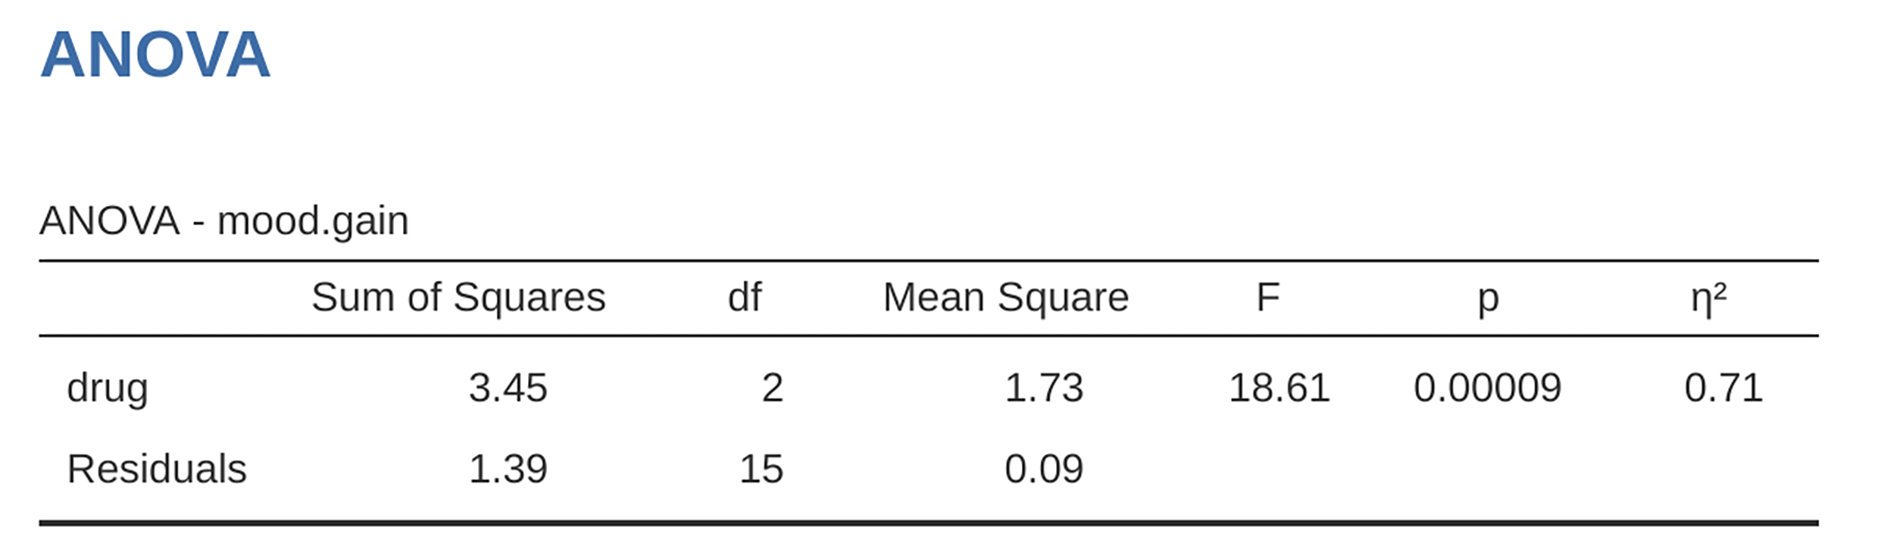
\includegraphics[width=1\textwidth,height=\textheight]{images/fig13-3.png} \hfill{}

\caption{\label{fig-fig13-3}jamovi results table for ANOVA of mood gain
by drug administered}

\end{figure}

The jamovi results table shows you the sums of squares values, the
degrees of freedom, and a couple of other quantities that we're not
really interested in right now. Notice, however, that jamovi doesn't use
the names ``between group'' and ``within group''. Instead, it tries to
assign more meaningful names. In our particular example, the between
groups variance corresponds to the effect that the drug has on the
outcome variable, and the within groups variance corresponds to the
``leftover'' variability so it calls that the residuals. If we compare
these numbers to the numbers that I calculated by hand in
\protect\hyperlink{a-worked-example}{A worked example}, you can see that
they're more or less the same, apart from rounding errors. The between
groups sums of squares is \(SS_b = 3.45\), the within groups sums of
squares is \(SS_w = 1.39\), and the degrees of freedom are \(2\) and
\(15\) respectively. We also get the \(F\)-value and the \(p\)-value
and, again, these are more or less the same, give or take rounding
errors, to the numbers that we calculated ourselves when doing it the
long and tedious way.

\hypertarget{effect-size}{%
\section{Effect size}\label{effect-size}}

There's a few different ways you could measure the effect size in an
ANOVA, but the most commonly used measures are \(\eta^2\) (eta squared)
and partial \(\eta^2\). For a one-way analysis of variance they're
identical to each other, so for the moment I'll just explain \(\eta^2\).
The definition of \(\eta^2\) is actually really simple:
\[\eta^2=\frac{SS_b}{SS_{tot}}\]

That's all it is. So when I look at the ANOVA table in
Figure~\ref{fig-fig13-3}, I see that \(SS_b = 3.45\) and
\(SS_tot = 3.45 + 1.39 = 4.84\). Thus we get an \(\eta^2\) value of:
\[\eta^2=\frac{3.45}{4.84}=0.71\]

The interpretation of \(\eta^2\) is equally straightforward. It refers
to the proportion of the variability in the outcome variable (mood.gain)
that can be explained in terms of the predictor (drug). A value of
\(\eta^2=0\) means that there is no relationship at all between the two,
whereas a value of \(\eta^2=1\) means that the relationship is perfect.
Better yet, the \(\eta^2\) value is very closely related to \(R^2\), as
discussed previously in \textbf{?@sec-The-R2-value}, and has an
equivalent interpretation. Although many statistics textbooks suggest
\(\eta^2\) as the default effect size measure in ANOVA, there's an
interesting blog post\footnote{\url{https://daniellakens.blogspot.com/2015/06/why-you-should-use-omega-squared.html}}
by Daniel Lakens suggesting that eta-squared is perhaps not the best
measure of effect size in real-world data analysis, because it can be a
biased estimator. Usefully, there is also an option in jamovi to specify
omega-squared (\(\omega^2\)), which is less biased, alongside
eta-squared.

\hypertarget{multiple-comparisons-and-post-hoc-tests}{%
\section{Multiple comparisons and post hoc
tests}\label{multiple-comparisons-and-post-hoc-tests}}

Any time you run an ANOVA with more than two groups and you end up with
a significant effect, the first thing you'll probably want to ask is
which groups are actually different from one another. In our drugs
example, our null hypothesis was that all three drugs (placebo, Anxifree
and Joyzepam) have the exact same effect on mood. But if you think about
it, the null hypothesis is actually claiming three different things all
at once here. Specifically, it claims that:

\begin{itemize}
\tightlist
\item
  Your competitor's drug (Anxifree) is no better than a placebo (i.e.,
  \(\mu_A = \mu_P\) )
\item
  Your drug (Joyzepam) is no better than a placebo (i.e.,
  \(\mu_J = \mu_P\) )
\item
  Anxifree and Joyzepam are equally effective (i.e., \(\mu_J = \mu_A\))
\end{itemize}

If any one of those three claims is false, then the null hypothesis is
also false. So, now that we've rejected our null hypothesis, we're
thinking that at least one of those things isn't true. But which ones?
All three of these propositions are of interest. Since you certainly
want to know if your new drug Joyzepam is better than a placebo, it
would be nice to know how well it stacks up against an existing
commercial alternative (i.e., Anxifree). It would even be useful to
check the performance of Anxifree against the placebo. Even if Anxifree
has already been extensively tested against placebos by other
researchers, it can still be very useful to check that your study is
producing similar results to earlier work.

When we characterise the null hypothesis in terms of these three
distinct propositions, it becomes clear that there are eight possible
``states of the world'' that we need to distinguish between
(Table~\ref{tbl-tab13-9}).

\hypertarget{tbl-tab13-9}{}
 
  \providecommand{\huxb}[2]{\arrayrulecolor[RGB]{#1}\global\arrayrulewidth=#2pt}
  \providecommand{\huxvb}[2]{\color[RGB]{#1}\vrule width #2pt}
  \providecommand{\huxtpad}[1]{\rule{0pt}{#1}}
  \providecommand{\huxbpad}[1]{\rule[-#1]{0pt}{#1}}

\begin{table}[ht]
\caption{\label{tbl-tab13-9}The null hypothesis and eight possible ``states of the world'' }\tabularnewline

\begin{centerbox}
\begin{threeparttable}
\setlength{\tabcolsep}{0pt}
\begin{tabularx}{0.9\textwidth}{p{0.18\textwidth} p{0.18\textwidth} p{0.18\textwidth} p{0.18\textwidth} p{0.18\textwidth}}


\hhline{>{\huxb{0, 0, 0}{0.4}}->{\huxb{0, 0, 0}{0.4}}->{\huxb{0, 0, 0}{0.4}}->{\huxb{0, 0, 0}{0.4}}->{\huxb{0, 0, 0}{0.4}}-}
\arrayrulecolor{black}

\multicolumn{1}{!{\huxvb{0, 0, 0}{0}}p{0.18\textwidth}!{\huxvb{0, 0, 0}{0}}}{\hspace{0pt}\parbox[b]{0.18\textwidth-0pt-12pt}{\huxtpad{2pt + 1em}\centering \textbf{possibility:}\huxbpad{2pt}}} &
\multicolumn{1}{p{0.18\textwidth}!{\huxvb{0, 0, 0}{0}}}{\hspace{12pt}\parbox[b]{0.18\textwidth-12pt-12pt}{\huxtpad{2pt + 1em}\centering \textbf{is \( \mu_P = \mu_A \)?}\huxbpad{2pt}}} &
\multicolumn{1}{p{0.18\textwidth}!{\huxvb{0, 0, 0}{0}}}{\hspace{12pt}\parbox[b]{0.18\textwidth-12pt-12pt}{\huxtpad{2pt + 1em}\centering \textbf{is \( \mu_P = \mu_J \)?}\huxbpad{2pt}}} &
\multicolumn{1}{p{0.18\textwidth}!{\huxvb{0, 0, 0}{0}}}{\hspace{12pt}\parbox[b]{0.18\textwidth-12pt-12pt}{\huxtpad{2pt + 1em}\centering \textbf{is \( \mu_A = \mu_J \)?}\huxbpad{2pt}}} &
\multicolumn{1}{p{0.18\textwidth}!{\huxvb{0, 0, 0}{0}}}{\hspace{12pt}\parbox[b]{0.18\textwidth-12pt-0pt}{\huxtpad{2pt + 1em}\centering \textbf{which hypothesis?}\huxbpad{2pt}}} \tabularnewline[-0.5pt]


\hhline{>{\huxb{0, 0, 0}{0.4}}->{\huxb{0, 0, 0}{0.4}}->{\huxb{0, 0, 0}{0.4}}->{\huxb{0, 0, 0}{0.4}}->{\huxb{0, 0, 0}{0.4}}-}
\arrayrulecolor{black}

\multicolumn{1}{!{\huxvb{0, 0, 0}{0}}p{0.18\textwidth}!{\huxvb{0, 0, 0}{0}}}{\hspace{0pt}\parbox[b]{0.18\textwidth-0pt-12pt}{\huxtpad{2pt + 1em}\centering 1\huxbpad{2pt}}} &
\multicolumn{1}{p{0.18\textwidth}!{\huxvb{0, 0, 0}{0}}}{\hspace{12pt}\parbox[b]{0.18\textwidth-12pt-12pt}{\huxtpad{2pt + 1em}\centering \( \checkmark \)\huxbpad{2pt}}} &
\multicolumn{1}{p{0.18\textwidth}!{\huxvb{0, 0, 0}{0}}}{\hspace{12pt}\parbox[b]{0.18\textwidth-12pt-12pt}{\huxtpad{2pt + 1em}\centering \( \checkmark \)\huxbpad{2pt}}} &
\multicolumn{1}{p{0.18\textwidth}!{\huxvb{0, 0, 0}{0}}}{\hspace{12pt}\parbox[b]{0.18\textwidth-12pt-12pt}{\huxtpad{2pt + 1em}\centering \( \checkmark \)\huxbpad{2pt}}} &
\multicolumn{1}{p{0.18\textwidth}!{\huxvb{0, 0, 0}{0}}}{\hspace{12pt}\parbox[b]{0.18\textwidth-12pt-0pt}{\huxtpad{2pt + 1em}\centering null\huxbpad{2pt}}} \tabularnewline[-0.5pt]


\hhline{}
\arrayrulecolor{black}

\multicolumn{1}{!{\huxvb{0, 0, 0}{0}}p{0.18\textwidth}!{\huxvb{0, 0, 0}{0}}}{\hspace{0pt}\parbox[b]{0.18\textwidth-0pt-12pt}{\huxtpad{2pt + 1em}\centering 2\huxbpad{2pt}}} &
\multicolumn{1}{p{0.18\textwidth}!{\huxvb{0, 0, 0}{0}}}{\hspace{12pt}\parbox[b]{0.18\textwidth-12pt-12pt}{\huxtpad{2pt + 1em}\centering \( \checkmark \)\huxbpad{2pt}}} &
\multicolumn{1}{p{0.18\textwidth}!{\huxvb{0, 0, 0}{0}}}{\hspace{12pt}\parbox[b]{0.18\textwidth-12pt-12pt}{\huxtpad{2pt + 1em}\centering \( \checkmark \)\huxbpad{2pt}}} &
\multicolumn{1}{p{0.18\textwidth}!{\huxvb{0, 0, 0}{0}}}{\hspace{12pt}\parbox[b]{0.18\textwidth-12pt-12pt}{\huxtpad{2pt + 1em}\centering \huxbpad{2pt}}} &
\multicolumn{1}{p{0.18\textwidth}!{\huxvb{0, 0, 0}{0}}}{\hspace{12pt}\parbox[b]{0.18\textwidth-12pt-0pt}{\huxtpad{2pt + 1em}\centering alternative\huxbpad{2pt}}} \tabularnewline[-0.5pt]


\hhline{}
\arrayrulecolor{black}

\multicolumn{1}{!{\huxvb{0, 0, 0}{0}}p{0.18\textwidth}!{\huxvb{0, 0, 0}{0}}}{\hspace{0pt}\parbox[b]{0.18\textwidth-0pt-12pt}{\huxtpad{2pt + 1em}\centering 3\huxbpad{2pt}}} &
\multicolumn{1}{p{0.18\textwidth}!{\huxvb{0, 0, 0}{0}}}{\hspace{12pt}\parbox[b]{0.18\textwidth-12pt-12pt}{\huxtpad{2pt + 1em}\centering \( \checkmark \)\huxbpad{2pt}}} &
\multicolumn{1}{p{0.18\textwidth}!{\huxvb{0, 0, 0}{0}}}{\hspace{12pt}\parbox[b]{0.18\textwidth-12pt-12pt}{\huxtpad{2pt + 1em}\centering \huxbpad{2pt}}} &
\multicolumn{1}{p{0.18\textwidth}!{\huxvb{0, 0, 0}{0}}}{\hspace{12pt}\parbox[b]{0.18\textwidth-12pt-12pt}{\huxtpad{2pt + 1em}\centering \( \checkmark \)\huxbpad{2pt}}} &
\multicolumn{1}{p{0.18\textwidth}!{\huxvb{0, 0, 0}{0}}}{\hspace{12pt}\parbox[b]{0.18\textwidth-12pt-0pt}{\huxtpad{2pt + 1em}\centering alternative\huxbpad{2pt}}} \tabularnewline[-0.5pt]


\hhline{}
\arrayrulecolor{black}

\multicolumn{1}{!{\huxvb{0, 0, 0}{0}}p{0.18\textwidth}!{\huxvb{0, 0, 0}{0}}}{\hspace{0pt}\parbox[b]{0.18\textwidth-0pt-12pt}{\huxtpad{2pt + 1em}\centering 4\huxbpad{2pt}}} &
\multicolumn{1}{p{0.18\textwidth}!{\huxvb{0, 0, 0}{0}}}{\hspace{12pt}\parbox[b]{0.18\textwidth-12pt-12pt}{\huxtpad{2pt + 1em}\centering \( \checkmark \)\huxbpad{2pt}}} &
\multicolumn{1}{p{0.18\textwidth}!{\huxvb{0, 0, 0}{0}}}{\hspace{12pt}\parbox[b]{0.18\textwidth-12pt-12pt}{\huxtpad{2pt + 1em}\centering \huxbpad{2pt}}} &
\multicolumn{1}{p{0.18\textwidth}!{\huxvb{0, 0, 0}{0}}}{\hspace{12pt}\parbox[b]{0.18\textwidth-12pt-12pt}{\huxtpad{2pt + 1em}\centering \huxbpad{2pt}}} &
\multicolumn{1}{p{0.18\textwidth}!{\huxvb{0, 0, 0}{0}}}{\hspace{12pt}\parbox[b]{0.18\textwidth-12pt-0pt}{\huxtpad{2pt + 1em}\centering alternative\huxbpad{2pt}}} \tabularnewline[-0.5pt]


\hhline{}
\arrayrulecolor{black}

\multicolumn{1}{!{\huxvb{0, 0, 0}{0}}p{0.18\textwidth}!{\huxvb{0, 0, 0}{0}}}{\hspace{0pt}\parbox[b]{0.18\textwidth-0pt-12pt}{\huxtpad{2pt + 1em}\centering 5\huxbpad{2pt}}} &
\multicolumn{1}{p{0.18\textwidth}!{\huxvb{0, 0, 0}{0}}}{\hspace{12pt}\parbox[b]{0.18\textwidth-12pt-12pt}{\huxtpad{2pt + 1em}\centering \( \checkmark \)\huxbpad{2pt}}} &
\multicolumn{1}{p{0.18\textwidth}!{\huxvb{0, 0, 0}{0}}}{\hspace{12pt}\parbox[b]{0.18\textwidth-12pt-12pt}{\huxtpad{2pt + 1em}\centering \( \checkmark \)\huxbpad{2pt}}} &
\multicolumn{1}{p{0.18\textwidth}!{\huxvb{0, 0, 0}{0}}}{\hspace{12pt}\parbox[b]{0.18\textwidth-12pt-12pt}{\huxtpad{2pt + 1em}\centering \( \checkmark \)\huxbpad{2pt}}} &
\multicolumn{1}{p{0.18\textwidth}!{\huxvb{0, 0, 0}{0}}}{\hspace{12pt}\parbox[b]{0.18\textwidth-12pt-0pt}{\huxtpad{2pt + 1em}\centering alternative\huxbpad{2pt}}} \tabularnewline[-0.5pt]


\hhline{}
\arrayrulecolor{black}

\multicolumn{1}{!{\huxvb{0, 0, 0}{0}}p{0.18\textwidth}!{\huxvb{0, 0, 0}{0}}}{\hspace{0pt}\parbox[b]{0.18\textwidth-0pt-12pt}{\huxtpad{2pt + 1em}\centering 6\huxbpad{2pt}}} &
\multicolumn{1}{p{0.18\textwidth}!{\huxvb{0, 0, 0}{0}}}{\hspace{12pt}\parbox[b]{0.18\textwidth-12pt-12pt}{\huxtpad{2pt + 1em}\centering \huxbpad{2pt}}} &
\multicolumn{1}{p{0.18\textwidth}!{\huxvb{0, 0, 0}{0}}}{\hspace{12pt}\parbox[b]{0.18\textwidth-12pt-12pt}{\huxtpad{2pt + 1em}\centering \( \checkmark \)\huxbpad{2pt}}} &
\multicolumn{1}{p{0.18\textwidth}!{\huxvb{0, 0, 0}{0}}}{\hspace{12pt}\parbox[b]{0.18\textwidth-12pt-12pt}{\huxtpad{2pt + 1em}\centering \huxbpad{2pt}}} &
\multicolumn{1}{p{0.18\textwidth}!{\huxvb{0, 0, 0}{0}}}{\hspace{12pt}\parbox[b]{0.18\textwidth-12pt-0pt}{\huxtpad{2pt + 1em}\centering alternative\huxbpad{2pt}}} \tabularnewline[-0.5pt]


\hhline{}
\arrayrulecolor{black}

\multicolumn{1}{!{\huxvb{0, 0, 0}{0}}p{0.18\textwidth}!{\huxvb{0, 0, 0}{0}}}{\hspace{0pt}\parbox[b]{0.18\textwidth-0pt-12pt}{\huxtpad{2pt + 1em}\centering 7\huxbpad{2pt}}} &
\multicolumn{1}{p{0.18\textwidth}!{\huxvb{0, 0, 0}{0}}}{\hspace{12pt}\parbox[b]{0.18\textwidth-12pt-12pt}{\huxtpad{2pt + 1em}\centering \huxbpad{2pt}}} &
\multicolumn{1}{p{0.18\textwidth}!{\huxvb{0, 0, 0}{0}}}{\hspace{12pt}\parbox[b]{0.18\textwidth-12pt-12pt}{\huxtpad{2pt + 1em}\centering \huxbpad{2pt}}} &
\multicolumn{1}{p{0.18\textwidth}!{\huxvb{0, 0, 0}{0}}}{\hspace{12pt}\parbox[b]{0.18\textwidth-12pt-12pt}{\huxtpad{2pt + 1em}\centering \( \checkmark \)\huxbpad{2pt}}} &
\multicolumn{1}{p{0.18\textwidth}!{\huxvb{0, 0, 0}{0}}}{\hspace{12pt}\parbox[b]{0.18\textwidth-12pt-0pt}{\huxtpad{2pt + 1em}\centering alternative\huxbpad{2pt}}} \tabularnewline[-0.5pt]


\hhline{}
\arrayrulecolor{black}

\multicolumn{1}{!{\huxvb{0, 0, 0}{0}}p{0.18\textwidth}!{\huxvb{0, 0, 0}{0}}}{\hspace{0pt}\parbox[b]{0.18\textwidth-0pt-12pt}{\huxtpad{2pt + 1em}\centering 8\huxbpad{2pt}}} &
\multicolumn{1}{p{0.18\textwidth}!{\huxvb{0, 0, 0}{0}}}{\hspace{12pt}\parbox[b]{0.18\textwidth-12pt-12pt}{\huxtpad{2pt + 1em}\centering \huxbpad{2pt}}} &
\multicolumn{1}{p{0.18\textwidth}!{\huxvb{0, 0, 0}{0}}}{\hspace{12pt}\parbox[b]{0.18\textwidth-12pt-12pt}{\huxtpad{2pt + 1em}\centering \huxbpad{2pt}}} &
\multicolumn{1}{p{0.18\textwidth}!{\huxvb{0, 0, 0}{0}}}{\hspace{12pt}\parbox[b]{0.18\textwidth-12pt-12pt}{\huxtpad{2pt + 1em}\centering \huxbpad{2pt}}} &
\multicolumn{1}{p{0.18\textwidth}!{\huxvb{0, 0, 0}{0}}}{\hspace{12pt}\parbox[b]{0.18\textwidth-12pt-0pt}{\huxtpad{2pt + 1em}\centering alternative\huxbpad{2pt}}} \tabularnewline[-0.5pt]


\hhline{>{\huxb{0, 0, 0}{0.4}}->{\huxb{0, 0, 0}{0.4}}->{\huxb{0, 0, 0}{0.4}}->{\huxb{0, 0, 0}{0.4}}->{\huxb{0, 0, 0}{0.4}}-}
\arrayrulecolor{black}
\end{tabularx} 

\end{threeparttable}\par\end{centerbox}

\end{table}
 

By rejecting the null hypothesis, we've decided that we don't believe
that \#1 is the true state of the world. The next question to ask is,
which of the other seven possibilities \emph{do} we think is right? When
faced with this situation, it's usually helps to look at the data. For
instance, if we look at the plots in Figure~\ref{fig-fig13-1}, it's
tempting to conclude that Joyzepam is better than the placebo and better
than Anxifree, but there's no real difference between Anxifree and the
placebo. However, if we want to get a clearer answer about this, it
might help to run some tests.

\hypertarget{running-pairwise-t-tests}{%
\subsection{\texorpdfstring{Running ``pairwise''
\(t\)-tests}{Running ``pairwise'' t-tests}}\label{running-pairwise-t-tests}}

How might we go about solving our problem? Given that we've got three
separate pairs of means (placebo versus Anxifree, placebo versus
Joyzepam, and Anxifree versus Joyzepam) to compare, what we could do is
run three separate \(t\)-tests and see what happens. This is easy to do
in jamovi. Go to the ANOVA `Post Hoc Tests' options, move the `drug'
variable across into the active box on the right, and then click on the
`No correction' checkbox. This will produce a neat table showing all the
pairwise \(t\)-test comparisons amongst the three levels of the drug
variable, as in Figure~\ref{fig-fig13-4}.

\begin{figure}

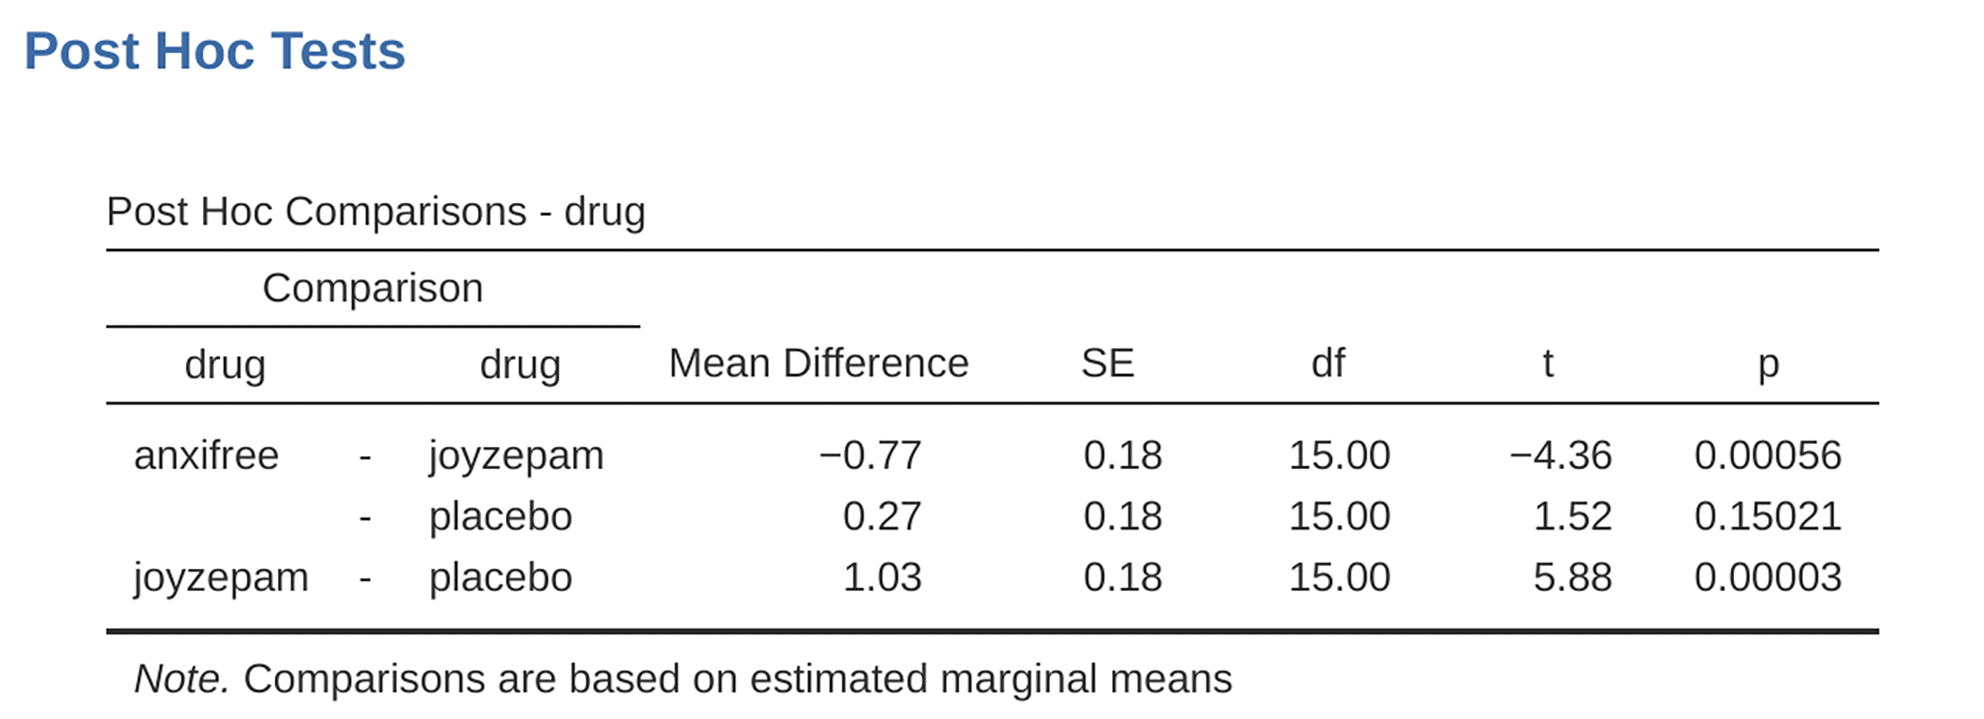
\includegraphics[width=1\textwidth,height=\textheight]{images/fig13-4.png} \hfill{}

\caption{\label{fig-fig13-4}Uncorrected pairwise \(t\)-tests as post hoc
comparisons in jamovi}

\end{figure}

\hypertarget{corrections-for-multiple-testing}{%
\subsection{Corrections for multiple
testing}\label{corrections-for-multiple-testing}}

In the previous section I hinted that there's a problem with just
running lots and lots of \(t\)-tests. The concern is that, when running
these analyses, what we're doing is going on a ``fishing expedition''.
We're running lots and lots of tests without much theoretical guidance
in the hope that some of them come up significant. This kind of
theory-free search for group differences is referred to as \textbf{post
hoc analysis} (``post hoc'' being Latin for ``after this'').\footnote{If
  you \emph{do} have some theoretical basis for wanting to investigate
  some comparisons but not others, it's a different story. In those
  circumstances you're not really running ``post hoc'' analyses at all,
  you're making ``planned comparisons''. I do talk about this situation
  later in the book - \textbf{?@sec-The-method-of-planned-comparisons},
  but for now I want to keep things simple.}

It's okay to run post hoc analyses, but a lot of care is required. For
instance, the analysis that I ran in the previous section should be
avoided, as each individual \(t\)-test is designed to have a 5\% type I
error rate (i.e., \(\alpha = .05\)) and I ran three of these tests.
Imagine what would have happened if my ANOVA involved 10 different
groups, and I had decided to run 45 ``post hoc'' \(t\)-tests to try to
find out which ones were significantly different from each other, you'd
expect 2 or 3 of them to come up significant by chance alone. As we saw
in \textbf{?@sec-Hypothesis-testing}, the central organising principle
behind null hypothesis testing is that we seek to control our type I
error rate, but now that I'm running lots of \(t\)-tests at once in
order to determine the source of my ANOVA results, my actual type I
error rate across this whole family of tests has gotten completely out
of control.

The usual solution to this problem is to introduce an adjustment to the
\(p\)-value, which aims to control the total error rate across the
family of tests (see Shaffer (1995)). An adjustment of this form, which
is usually (but not always) applied because one is doing post hoc
analysis, is often referred to as a \textbf{correction for multiple
comparisons}, though it is sometimes referred to as ``simultaneous
inference''. In any case, there are quite a few different ways of doing
this adjustment. I'll discuss a few of them in this section and in
\textbf{?@sec-Post-hoc-tests} in the next chapter, but you should be
aware that there are many other methods out there (see, e.g., Hsu
(1996)).

\hypertarget{bonferroni-corrections}{%
\subsection{Bonferroni corrections}\label{bonferroni-corrections}}

The simplest of these adjustments is called the \textbf{Bonferroni
correction} (Dunn, 1961), and it's very very simple indeed. Suppose that
my post hoc analysis consists of \(m\) separate tests, and I want to
ensure that the total probability of making \emph{any} type I errors at
all is at most \(\alpha\).\footnote{It's worth noting in passing that
  not all adjustment methods try to do this. What I've described here is
  an approach for controlling ``family wise type I error rate''.
  However, there are other post hoc tests that seek to control the
  ``false discovery rate'', which is a somewhat different thing:
  \[p_j^{'}=m \times p\] And therefore, if you're using the Bonferroni
  correction, you would reject the null hypothesis if
  \(p_j^{'} < \alpha\). The logic behind this correction is very
  straightforward. We're doing m different tests, so if we arrange it so
  that each test has a type I error rate of at most
  \(\frac{\alpha}{m}\), then the \emph{total} type I error rate across
  these tests cannot be larger than \(\alpha\). That's pretty simple, so
  much so that in the original paper, the author writes:} If so, then
the Bonferroni correction just says ``multiply all your raw \(p\)-values
by \(m\)''. If we let \(p\) denote the original \(p\)-value, and let
\(p_j^{'}\) be the corrected value, then the Bonferroni correction tells
that:

\begin{quote}
``\emph{The method given here is so simple and so general that I am sure
it must have been used before this. I do not find it, however, so can
only conclude that perhaps its very simplicity has kept statisticians
from realizing that it is a very good method in some situations}'' (Dunn
(1961), pp.~52-53).
\end{quote}

To use the Bonferroni correction in jamovi, just click on the
`Bonferroni' checkbox in the `Correction' options, and you will see
another column added to the ANOVA results table showing the adjusted
\(p\)-values for the Bonferroni correction (Table~\ref{tbl-tab13-8}). If
we compare these three \(p\)-values to those for the uncorrected,
pairwise \(t\)-tests, it is clear that the only thing that jamovi has
done is multiply them by \(3\).

\hypertarget{holm-corrections}{%
\subsection{Holm corrections}\label{holm-corrections}}

Although the Bonferroni correction is the simplest adjustment out there,
it's not usually the best one to use. One method that is often used
instead is the \textbf{Holm correction} (Holm, 1979). The idea behind
the Holm correction is to pretend that you're doing the tests
sequentially, starting with the smallest (raw) \(p\)-value and moving
onto the largest one. For the \(j\)-th largest of the \(p\)-values, the
adjustment is \emph{either}: \[p_j^{'}=j \times p_j\]

(i.e., the biggest \(p\)-value remains unchanged, the second biggest
\(p\)-value is doubled, the third biggest \(p\)-value is tripled, and so
on), or: \[p_j^{'}=p_{j+1}^{'}\]

whichever one is larger. This might sound a little confusing, so let's
go through it a little more slowly. Here's what the Holm correction
does. First, you sort all of your \(p\)-values in order, from smallest
to largest. For the smallest \(p\)-value all you do is multiply it by
\(m\), and you're done. However, for all the other ones it's a two-stage
process. For instance, when you move to the second smallest \(p\)-value,
you first multiply it by \(m - 1\). If this produces a number that is
bigger than the adjusted \(p\)-value that you got last time, then you
keep it. But if it's smaller than the last one, then you copy the last
\(p\)-value. To illustrate how this works, consider
Table~\ref{tbl-tab13-10} which shows the calculations of a Holm
correction for a collection of five \(p\)-values.

\hypertarget{tbl-tab13-10}{}
 
  \providecommand{\huxb}[2]{\arrayrulecolor[RGB]{#1}\global\arrayrulewidth=#2pt}
  \providecommand{\huxvb}[2]{\color[RGB]{#1}\vrule width #2pt}
  \providecommand{\huxtpad}[1]{\rule{0pt}{#1}}
  \providecommand{\huxbpad}[1]{\rule[-#1]{0pt}{#1}}

\begin{table}[ht]
\caption{\label{tbl-tab13-10}Holm corrected \(p\)-values }\tabularnewline

\begin{centerbox}
\begin{threeparttable}
\setlength{\tabcolsep}{0pt}
\begin{tabularx}{0.9\textwidth}{p{0.225\textwidth} p{0.225\textwidth} p{0.225\textwidth} p{0.225\textwidth}}


\hhline{>{\huxb{0, 0, 0}{0.4}}->{\huxb{0, 0, 0}{0.4}}->{\huxb{0, 0, 0}{0.4}}->{\huxb{0, 0, 0}{0.4}}-}
\arrayrulecolor{black}

\multicolumn{1}{!{\huxvb{0, 0, 0}{0}}p{0.225\textwidth}!{\huxvb{0, 0, 0}{0}}}{\hspace{0pt}\parbox[b]{0.225\textwidth-0pt-12pt}{\huxtpad{2pt + 1em}\centering \textbf{raw \( p \)}\huxbpad{2pt}}} &
\multicolumn{1}{p{0.225\textwidth}!{\huxvb{0, 0, 0}{0}}}{\hspace{12pt}\parbox[b]{0.225\textwidth-12pt-12pt}{\huxtpad{2pt + 1em}\centering \textbf{rank \( j \)}\huxbpad{2pt}}} &
\multicolumn{1}{p{0.225\textwidth}!{\huxvb{0, 0, 0}{0}}}{\hspace{12pt}\parbox[b]{0.225\textwidth-12pt-12pt}{\huxtpad{2pt + 1em}\centering \textbf{\( p \times j \)}\huxbpad{2pt}}} &
\multicolumn{1}{p{0.225\textwidth}!{\huxvb{0, 0, 0}{0}}}{\hspace{12pt}\parbox[b]{0.225\textwidth-12pt-0pt}{\huxtpad{2pt + 1em}\centering \textbf{Holm \( p \)}\huxbpad{2pt}}} \tabularnewline[-0.5pt]


\hhline{>{\huxb{0, 0, 0}{0.4}}->{\huxb{0, 0, 0}{0.4}}->{\huxb{0, 0, 0}{0.4}}->{\huxb{0, 0, 0}{0.4}}-}
\arrayrulecolor{black}

\multicolumn{1}{!{\huxvb{0, 0, 0}{0}}p{0.225\textwidth}!{\huxvb{0, 0, 0}{0}}}{\hspace{0pt}\parbox[b]{0.225\textwidth-0pt-12pt}{\huxtpad{2pt + 1em}\centering .001\huxbpad{2pt}}} &
\multicolumn{1}{p{0.225\textwidth}!{\huxvb{0, 0, 0}{0}}}{\hspace{12pt}\parbox[b]{0.225\textwidth-12pt-12pt}{\huxtpad{2pt + 1em}\centering 5\huxbpad{2pt}}} &
\multicolumn{1}{p{0.225\textwidth}!{\huxvb{0, 0, 0}{0}}}{\hspace{12pt}\parbox[b]{0.225\textwidth-12pt-12pt}{\huxtpad{2pt + 1em}\centering .005\huxbpad{2pt}}} &
\multicolumn{1}{p{0.225\textwidth}!{\huxvb{0, 0, 0}{0}}}{\hspace{12pt}\parbox[b]{0.225\textwidth-12pt-0pt}{\huxtpad{2pt + 1em}\centering .005\huxbpad{2pt}}} \tabularnewline[-0.5pt]


\hhline{}
\arrayrulecolor{black}

\multicolumn{1}{!{\huxvb{0, 0, 0}{0}}p{0.225\textwidth}!{\huxvb{0, 0, 0}{0}}}{\hspace{0pt}\parbox[b]{0.225\textwidth-0pt-12pt}{\huxtpad{2pt + 1em}\centering .005\huxbpad{2pt}}} &
\multicolumn{1}{p{0.225\textwidth}!{\huxvb{0, 0, 0}{0}}}{\hspace{12pt}\parbox[b]{0.225\textwidth-12pt-12pt}{\huxtpad{2pt + 1em}\centering 4\huxbpad{2pt}}} &
\multicolumn{1}{p{0.225\textwidth}!{\huxvb{0, 0, 0}{0}}}{\hspace{12pt}\parbox[b]{0.225\textwidth-12pt-12pt}{\huxtpad{2pt + 1em}\centering .020\huxbpad{2pt}}} &
\multicolumn{1}{p{0.225\textwidth}!{\huxvb{0, 0, 0}{0}}}{\hspace{12pt}\parbox[b]{0.225\textwidth-12pt-0pt}{\huxtpad{2pt + 1em}\centering .020\huxbpad{2pt}}} \tabularnewline[-0.5pt]


\hhline{}
\arrayrulecolor{black}

\multicolumn{1}{!{\huxvb{0, 0, 0}{0}}p{0.225\textwidth}!{\huxvb{0, 0, 0}{0}}}{\hspace{0pt}\parbox[b]{0.225\textwidth-0pt-12pt}{\huxtpad{2pt + 1em}\centering .019\huxbpad{2pt}}} &
\multicolumn{1}{p{0.225\textwidth}!{\huxvb{0, 0, 0}{0}}}{\hspace{12pt}\parbox[b]{0.225\textwidth-12pt-12pt}{\huxtpad{2pt + 1em}\centering 3\huxbpad{2pt}}} &
\multicolumn{1}{p{0.225\textwidth}!{\huxvb{0, 0, 0}{0}}}{\hspace{12pt}\parbox[b]{0.225\textwidth-12pt-12pt}{\huxtpad{2pt + 1em}\centering .057\huxbpad{2pt}}} &
\multicolumn{1}{p{0.225\textwidth}!{\huxvb{0, 0, 0}{0}}}{\hspace{12pt}\parbox[b]{0.225\textwidth-12pt-0pt}{\huxtpad{2pt + 1em}\centering .057\huxbpad{2pt}}} \tabularnewline[-0.5pt]


\hhline{}
\arrayrulecolor{black}

\multicolumn{1}{!{\huxvb{0, 0, 0}{0}}p{0.225\textwidth}!{\huxvb{0, 0, 0}{0}}}{\hspace{0pt}\parbox[b]{0.225\textwidth-0pt-12pt}{\huxtpad{2pt + 1em}\centering .022\huxbpad{2pt}}} &
\multicolumn{1}{p{0.225\textwidth}!{\huxvb{0, 0, 0}{0}}}{\hspace{12pt}\parbox[b]{0.225\textwidth-12pt-12pt}{\huxtpad{2pt + 1em}\centering 2\huxbpad{2pt}}} &
\multicolumn{1}{p{0.225\textwidth}!{\huxvb{0, 0, 0}{0}}}{\hspace{12pt}\parbox[b]{0.225\textwidth-12pt-12pt}{\huxtpad{2pt + 1em}\centering .044\huxbpad{2pt}}} &
\multicolumn{1}{p{0.225\textwidth}!{\huxvb{0, 0, 0}{0}}}{\hspace{12pt}\parbox[b]{0.225\textwidth-12pt-0pt}{\huxtpad{2pt + 1em}\centering .057\huxbpad{2pt}}} \tabularnewline[-0.5pt]


\hhline{}
\arrayrulecolor{black}

\multicolumn{1}{!{\huxvb{0, 0, 0}{0}}p{0.225\textwidth}!{\huxvb{0, 0, 0}{0}}}{\hspace{0pt}\parbox[b]{0.225\textwidth-0pt-12pt}{\huxtpad{2pt + 1em}\centering .103\huxbpad{2pt}}} &
\multicolumn{1}{p{0.225\textwidth}!{\huxvb{0, 0, 0}{0}}}{\hspace{12pt}\parbox[b]{0.225\textwidth-12pt-12pt}{\huxtpad{2pt + 1em}\centering 1\huxbpad{2pt}}} &
\multicolumn{1}{p{0.225\textwidth}!{\huxvb{0, 0, 0}{0}}}{\hspace{12pt}\parbox[b]{0.225\textwidth-12pt-12pt}{\huxtpad{2pt + 1em}\centering .103\huxbpad{2pt}}} &
\multicolumn{1}{p{0.225\textwidth}!{\huxvb{0, 0, 0}{0}}}{\hspace{12pt}\parbox[b]{0.225\textwidth-12pt-0pt}{\huxtpad{2pt + 1em}\centering .103\huxbpad{2pt}}} \tabularnewline[-0.5pt]


\hhline{>{\huxb{0, 0, 0}{0.4}}->{\huxb{0, 0, 0}{0.4}}->{\huxb{0, 0, 0}{0.4}}->{\huxb{0, 0, 0}{0.4}}-}
\arrayrulecolor{black}
\end{tabularx} 

\end{threeparttable}\par\end{centerbox}

\end{table}
 

Hopefully that makes things clear.

Although it's a little harder to calculate, the Holm correction has some
very nice properties. It's more powerful than Bonferroni (i.e., it has a
lower type II error rate) but, counter-intuitive as it might seem, it
has the same type I error rate. As a consequence, in practice there's
never any reason to use the simpler Bonferroni correction since it is
always outperformed by the slightly more elaborate Holm correction.
Because of this, the Holm correction should be your \emph{go to}
multiple comparison correction. Figure~\ref{fig-fig13-4} also shows the
Holm corrected \(p\)-values and, as you can see, the biggest \(p\)-value
(corresponding to the comparison between Anxifree and the placebo) is
unaltered. At a value of .15, it is exactly the same as the value we got
originally when we applied no correction at all. In contrast, the
smallest \(p\)-value (Joyzepam versus placebo) has been multiplied by
three.

\hypertarget{writing-up-the-post-hoc-test}{%
\subsection{Writing up the post hoc
test}\label{writing-up-the-post-hoc-test}}

Finally, having run the post hoc analysis to determine which groups are
significantly different to one another, you might write up the result
like this:

\begin{quote}
Post hoc tests (using the Holm correction to adjust \(p\)) indicated
that Joyzepam produced a significantly larger mood change than both
Anxifree (\(p = .001\)) and the placebo (\((p = 9.0 \times{10^{-5}}\)).
We found no evidence that Anxifree performed better than the placebo
(\(p = .15\)).
\end{quote}

Or, if you don't like the idea of reporting exact \(p\)-values, then
you'd change those numbers to \(p < .01\), \(p < .001\) and \(p > .05\)
respectively. Either way, the key thing is that you indicate that you
used Holm's correction to adjust the \(p\)-values. And of course, I'm
assuming that elsewhere in the write up you've included the relevant
descriptive statistics (i.e., the group means and standard deviations),
since these \(p\)-values on their own aren't terribly informative.

\hypertarget{the-assumptions-of-one-way-anova}{%
\section{The assumptions of one-way
ANOVA}\label{the-assumptions-of-one-way-anova}}

Like any statistical test, analysis of variance relies on some
assumptions about the data, specifically the residuals. There are three
key assumptions that you need to be aware of: normality, homogeneity of
variance and independence.

{[}Additional technical detail\footnote{If you remember back to
  \protect\hyperlink{a-worked-example}{A worked example}, which I hope
  you at least skimmed even if you didn't read the whole thing, I
  described the statistical models underpinning ANOVA in this way:
  \[H_0:Y_{ik}=\mu + \epsilon_{ik}\]
  \[H_1:Y_{ik}=\mu_k + \epsilon_{ik}\] In these equations \(\mu\) refers
  to a single grand population mean which is the same for all groups,
  and \(\mu\)k is the population mean for the k-th group. Up to this
  point we've been mostly interested in whether our data are best
  described in terms of a single grand mean (the null hypothesis) or in
  terms of different group-specific means (the alternative hypothesis).
  This makes sense, of course, as that's actually the important research
  question! However, all of our testing procedures have, implicitly,
  relied on a specific assumption about the residuals,
  \(\epsilon\_{ik}\), namely that:
  \[\epsilon_{ik} \sim Normal(0,\sigma^2)\] None of the maths works
  properly without this bit. Or, to be precise, you can still do all the
  calculations and you'll end up with an \(F\)-statistic, but you have
  no guarantee that this \(F\)-statistic actually measures what you
  think it's measuring, and so any conclusions that you might draw on
  the basis of the \(F\)-test might be wrong.}{]}

So, how do we check whether the assumption about the residuals is
accurate? Well, as I indicated above, there are three distinct claims
buried in this one statement, and we'll consider them separately.

\begin{itemize}
\tightlist
\item
  \textbf{Homogeneity of variance}. Notice that we've only got the one
  value for the population standard deviation (i.e., \(\sigma\)), rather
  than allowing each group to have it's own value (i.e., \(\sigma_k\)).
  This is referred to as the homogeneity of variance (sometimes called
  homoscedasticity) assumption. ANOVA assumes that the population
  standard deviation is the same for all groups. We'll talk about this
  extensively in the
  \protect\hyperlink{sec-Checking-the-homogeneity-of-variance-assumption}{Checking
  the homogeneity of variance assumption} section.
\item
  \textbf{Normality}. The residuals are assumed to be normally
  distributed. As we saw in
  \textbf{?@sec-Checking-the-normality-of-a-sample}, we can assess this
  by looking at QQ plots (or running a Shapiro-Wilk test. I'll talk
  about this more in an ANOVA context in the
  \protect\hyperlink{sec-Checking-the-normality-assumption}{Checking the
  normality assumption} section.
\item
  \textbf{Independence}. The independence assumption is a little
  trickier. What it basically means is that, knowing one residual tells
  you nothing about any other residual. All of the \(\epsilon_{ik}\)
  values are assumed to have been generated without any ``regard for''
  or ``relationship to'' any of the other ones. There's not an obvious
  or simple way to test for this, but there are some situations that are
  clear violations of this. For instance, if you have a repeated
  measures design, where each participant in your study appears in more
  than one condition, then independence doesn't hold. There's a special
  relationship between some observations, namely those that correspond
  to the same person! When that happens, you need to use something like
  a \protect\hyperlink{repeated-measures-one-way-anova}{Repeated
  measures one-way ANOVA}.
\end{itemize}

\hypertarget{sec-Checking-the-homogeneity-of-variance-assumption}{%
\subsection{Checking the homogeneity of variance
assumption}\label{sec-Checking-the-homogeneity-of-variance-assumption}}

\begin{quote}
\emph{To make the preliminary test on variances is rather like putting
to sea in a rowing boat to find out whether conditions are sufficiently
calm for an ocean liner to leave port!}\\
-- George Box (Box, 1953)
\end{quote}

There's more than one way to skin a cat, as the saying goes, and more
than one way to test the homogeneity of variance assumption, too (though
for some reason no-one made a saying out of that). The most commonly
used test for this that I've seen in the literature is the Levene test
(Levene, 1960), and the closely related Brown-Forsythe test (Brown \&
Forsythe, 1974).

Regardless of whether you're doing the standard Levene test or the
Brown-Forsythe test, the test statistic, which is sometimes denoted
\(F\) but also sometimes written as \(W\), is calculated in exactly the
same way that the \(F\)-statistic for the regular ANOVA is calculated,
just using a \(Z_{ik}\) rather than \(Y_{ik}\). With that in mind, we
can go on to look at how to run the test in jamovi.

{[}Additional technical detail\footnote{The Levene test is shockingly
  simple. Suppose we have our outcome variable \(Y_{ik}\). All we do is
  define a new variable, which I'll call \(Z_{ik}\), corresponding to
  the absolute deviation from the group mean:
  \[Z_{ik}=Y_{ik}-\bar{Y}_{k}\] Okay, what good does this do us? Well,
  let's take a moment to think about what \(Z_{ik}\) actually is and
  what we're trying to test. The value of \(Z_{ik}\) is a measure of how
  the \(i\)-th observation in the \(k\)-th group deviates from its group
  mean. And our null hypothesis is that all groups have the same
  variance, i.e., the same overall deviations from the group means! So
  the null hypothesis in a Levene test is that the population means of
  \(Z\) are identical for all groups. Hmm. So what we need now is a
  statistical test of the null hypothesis that all group means are
  identical. Where have we seen that before? Oh right, that's what ANOVA
  is, and so all that the Levene test does is run an ANOVA on the new
  variable \(Z_{ik}\). What about the Brown-Forsythe test? Does that do
  anything particularly different? Nope. The only change from the Levene
  test is that it constructs the transformed variable \(Z\) in a
  slightly different way, using deviations from the group medians rather
  than deviations from the group means. That is, for the Brown-Forsythe
  test: \[Z_{ik}=Y_{ik}-median_k(Y)\] where \(median_k(Y)\) is the
  median for group \(k\).}{]}

\hypertarget{running-the-levene-test-in-jamovi}{%
\subsection{Running the Levene test in
jamovi}\label{running-the-levene-test-in-jamovi}}

Okay, so how do we run the Levene test? Simple really -- under the ANOVA
`Assumption Checks' option, just click on the `Homogeneity tests'
checkbox. If we look at the output, shown in Figure~\ref{fig-fig13-5},
we see that the test is non-significant (\(F_{2,15} = 1.45, p = .266\)),
so it looks like the homogeneity of variance assumption is fine.
However, looks can be deceptive! If your sample size is pretty big, then
the Levene test could show up a significant effect (i.e.~p \textless{}
.05) even when the homogeneity of variance assumption is not violated to
an extent which troubles the robustness of ANOVA. This was the point
George Box was making in the quote above. Similarly, if your sample size
is quite small, then the homogeneity of variance assumption might not be
satisfied and yet a Levene test could be non-significant (i.e.~p
\textgreater{} .05). What this means is that, alongside any statistical
test of the assumption being met, you should always plot the standard
deviation around the means for each group / category in the
analysis\ldots just to see if they look fairly similar (i.e.~homogeneity
of variance) or not.

\begin{figure}

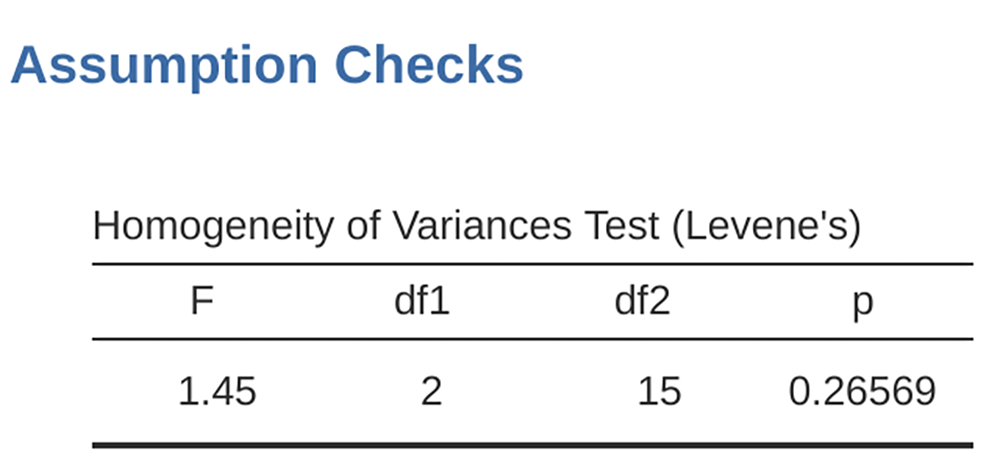
\includegraphics[width=1\textwidth,height=\textheight]{images/fig13-5.png} \hfill{}

\caption{\label{fig-fig13-5}Levene test output for one-way ANOVA in
jamovi}

\end{figure}

\hypertarget{removing-the-homogeneity-of-variance-assumption}{%
\subsection{Removing the homogeneity of variance
assumption}\label{removing-the-homogeneity-of-variance-assumption}}

In our example, the homogeneity of variance assumption turned out to be
a pretty safe one: the Levene test came back non-significant
(notwithstanding that we should also look at the plot of standard
deviations), so we probably don't need to worry. However, in real life
we aren't always that lucky. How do we save our ANOVA when the
homogeneity of variance assumption is violated? If you recall from our
discussion of \(t\)-tests, we've seen this problem before. The Student
\(t\)-test assumes equal variances, so the solution was to use the Welch
\(t\)-test, which does not. In fact, Welch (1951) also showed how we can
solve this problem for ANOVA too (the \textbf{Welch one-way test}). It's
implemented in jamovi using the One-Way ANOVA analysis. This is a
specific analysis approach just for one-way ANOVA, and to run the Welch
one-way ANOVA for our example, we would re-run the analysis as
previously, but this time use the jamovi ANOVA - one-way ANOVA analysis
command, and check the option for Welch's test (see
Figure~\ref{fig-fig13-6}). To understand what's happening here, let's
compare these numbers to what we got earlier when
\protect\hyperlink{running-an-anova-in-jamovi}{Running an ANOVA in
jamovi} originally. To save you the trouble of flicking back, this is
what we got last time: \(F(2, 15) = 18.611, p = .00009\), also shown as
the Fisher's test in the One-Way ANOVA shown in
Figure~\ref{fig-fig13-6}.

\begin{figure}

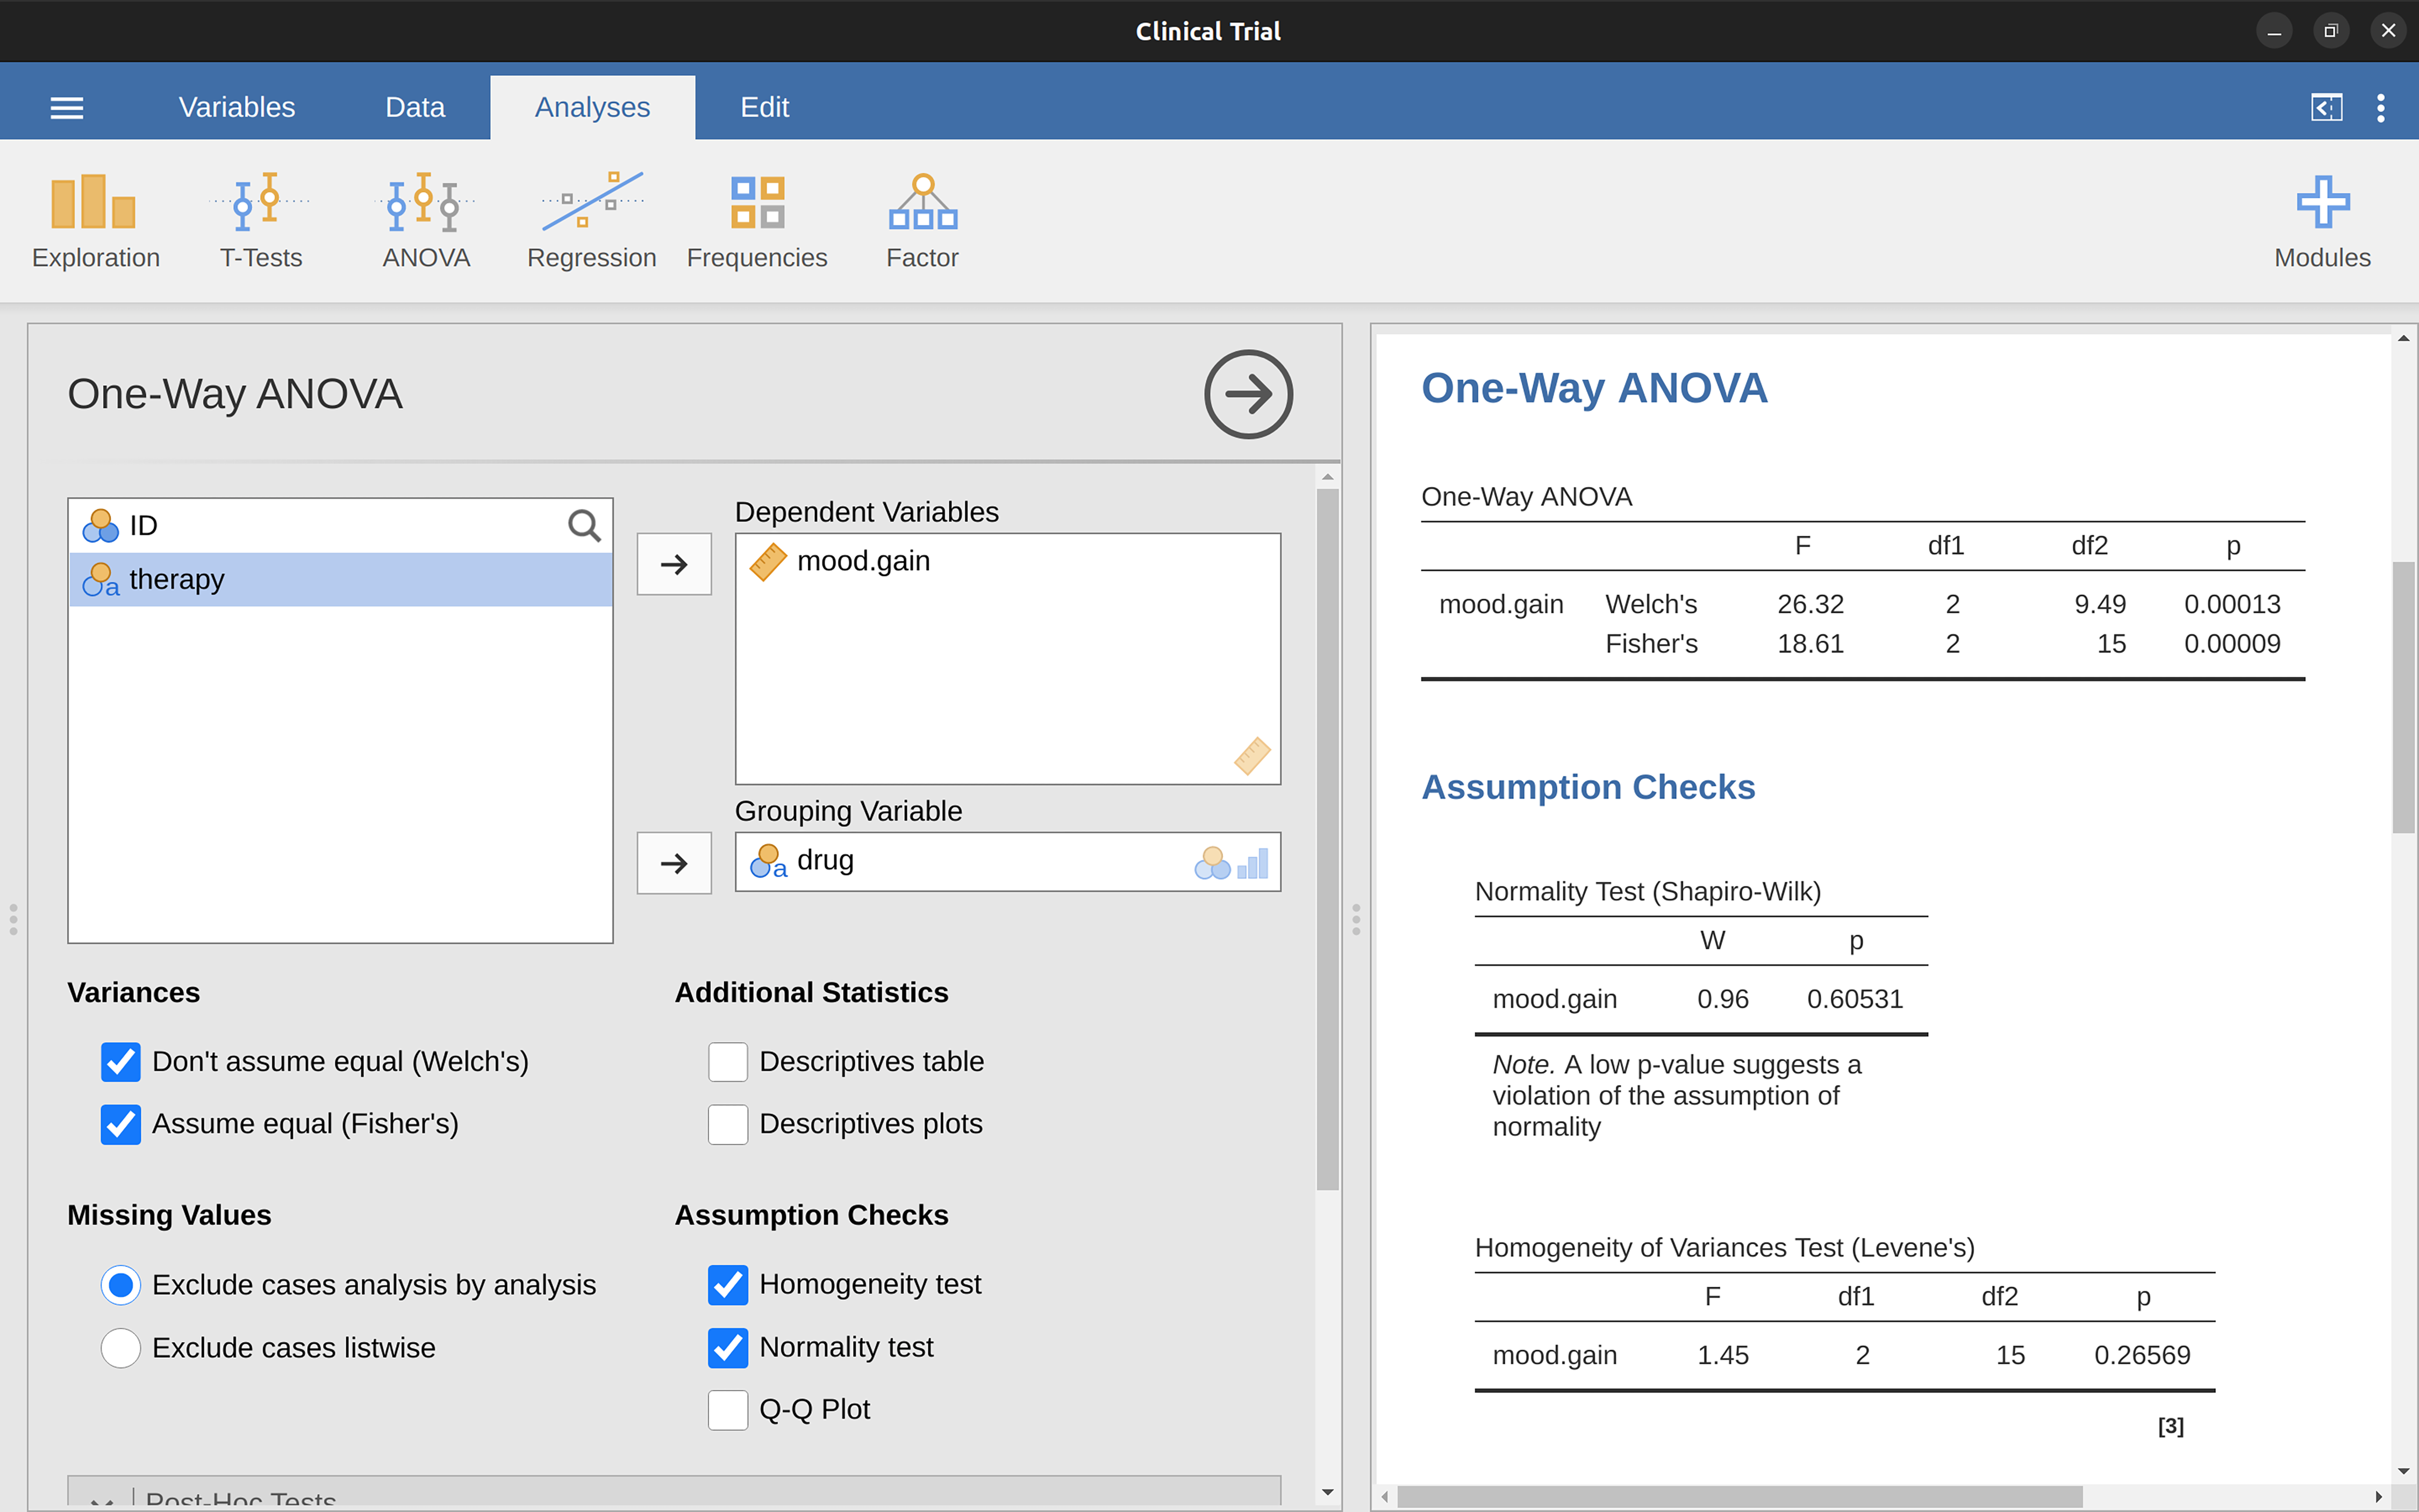
\includegraphics[width=1\textwidth,height=\textheight]{images/fig13-6.png} \hfill{}

\caption{\label{fig-fig13-6}Welch test as part of the one-way ANOVA
analysis in jamovi}

\end{figure}

Okay, so originally our ANOVA gave us the result \(F(2, 15) = 18.6\),
whereas the Welch one-way test gave us \(F(2, 9.49) = 26.32\). In other
words, the Welch test has reduced the within groups degrees of freedom
from 15 to 9.49, and the \(F\)-value has increased from 18.6 to 26.32.

\hypertarget{sec-Checking-the-normality-assumption}{%
\subsection{Checking the normality
assumption}\label{sec-Checking-the-normality-assumption}}

Testing the normality assumption is relatively straightforward. We
covered most of what you need to know in
\textbf{?@sec-Checking-the-normality-of-a-sample}. The only thing we
really need to do is draw a QQ plot and, in addition if it is available,
run the Shapiro-Wilk test. The QQ plot is shown in
Figure~\ref{fig-fig13-7} and it looks pretty normal to me. If the
Shapiro-Wilk test is not significant (i.e.~\(p > .05\)) then this
indicates that the assumption of normality is not violated. However, as
with Levene's test, if the sample size is large then a significant
Shapiro-Wilk test may in fact be a false positive, where the assumption
of normality is not violated in any substantive problematic sense for
the analysis. And, similarly, a very small sample can produce false
negatives. That's why a visual inspection of the QQ plot is important.

\begin{figure}


\includegraphics[width=1\textwidth,height=\textheight]{images/fig13-7.png} \hfill{}

\caption{\label{fig-fig13-7}QQ plot in the one-way ANOVA analysis in
jamovi}

\end{figure}

Alongside inspecting the QQ plot for any deviations from normality, the
Shapiro-Wilk test for our data does show a non-significant effect, with
\(p\) = 0.6053 (see Figure~\ref{fig-fig13-6}). This therefore supports
the QQ plot assessment; both checks find no indication that normality is
violated.

\hypertarget{removing-the-normality-assumption}{%
\subsection{Removing the normality
assumption}\label{removing-the-normality-assumption}}

Now that we've seen how to check for normality, we are led naturally to
ask what we can do to address violations of normality. In the context of
a one-way ANOVA, the easiest solution is probably to switch to a
non-parametric test (i.e., one that doesn't rely on any particular
assumption about the kind of distribution involved). We've seen
non-parametric tests before, in \textbf{?@sec-Comparing-two-means}. When
you only have two groups, the Mann-Whitney or the Wilcoxon test provides
the non-parametric alternative that you need. When you've got three or
more groups, you can use the \textbf{Kruskal-Wallis rank sum test}
(Kruskal \& Wallis, 1952). So that's the test we'll talk about next.

\hypertarget{the-logic-behind-the-kruskal-wallis-test}{%
\subsection{The logic behind the Kruskal-Wallis
test}\label{the-logic-behind-the-kruskal-wallis-test}}

The Kruskal-Wallis test is surprisingly similar to ANOVA, in some ways.
In ANOVA we started with \(Y_{ik}\), the value of the outcome variable
for the ith person in the kth group. For the Kruskal-Wallis test what
we'll do is rank order all of these \(Y_{ik}\) values and conduct our
analysis on the ranked data.\footnote{So let's let \(R\_{ik}\) refer to
  the ranking given to the \(i\)th member of the \(k\)th group. Now,
  let's calculate \(\bar{R}_k\), the average rank given to observations
  in the \(k\)th group: \[\bar{R}_k=\frac{1}{N_k}\sum_i R_{ik}\] and
  let's also calculate \(\bar{R}\), the grand mean rank:
  \[\bar{R}=\frac{1}{N}\sum_i\sum_k R_{ik}\] Now that we've done this,
  we can calculate the squared deviations from the grand mean rank
  \(\bar{R}\). When we do this for the individual scores, i.e., if we
  calculate \((R_{ik} - \bar{R})^2\) , what we have is a
  ``nonparametric'' measure of how far the \(ik\)-th observation
  deviates from the grand mean rank. When we calculate the squared
  deviation of the group means from the grand means, i.e., if we
  calculate \((R_{ik} - \bar{R})^2\), then what we have is a
  nonparametric measure of how much the group deviates from the grand
  mean rank. With this in mind, we'll follow the same logic that we did
  with ANOVA and define our ranked sums of squares measures, much like
  we did earlier. First, we have our ``total ranked sums of squares'':
  \[RSS_{tot}=\sum_k\sum_i (R_{ik}-\bar{R})^2\] and we can define the
  ``between groups ranked sums of squares'' like this:
  \[\begin{aligned} RSS_{b}& =\sum{k}\sum_{i}(\bar{R}_{k}-\bar{R})^2 \\ &= \sum_{k} N_k (\bar{R}_{k}-\bar{R})^2 \end{aligned}\]
  So, if the null hypothesis is true and there are no true group
  differences at all, you'd expect the between group rank sums \(RSS_b\)
  to be very small, much smaller than the total rank sums \(RSS_{tot}\).
  Qualitatively this is very much the same as what we found when we went
  about constructing the ANOVA \(F\)-statistic, but for technical
  reasons the Kruskal-Wallis test statistic, usually denoted \(K\), is
  constructed in a slightly different way:
  \[K=(N-1) \times \frac{RSS_b}{RSS_{tot}}\] and if the null hypothesis
  is true, then the sampling distribution of \(K\) is approximately
  chi-square with \(G-1\) degrees of freedom (where \(G\) is the number
  of groups). The larger the value of \(K\), the less consistent the
  data are with the null hypothesis, so this is a one-sided test. We
  reject \(H_0\) when \(K\) is sufficiently large.}

\hypertarget{additional-details}{%
\subsection{Additional details}\label{additional-details}}

The description in the previous section illustrates the logic behind the
Kruskal-Wallis test. At a conceptual level, this is the right way to
think about how the test works.\footnote{However, from a purely
  mathematical perspective it's needlessly complicated. I won't show you
  the derivation, but you can use a bit of algebraic
  jiggery-pokery\(^a\) to show that the equation for \(K\) can be:
  \[K=\frac{12}{N(N-1)}\sum_k N_k \bar{R}_k^2 -3(N+1)\] It's this last
  equation that you sometimes see given for \(K\). This is way easier to
  calculate than the version I described in the previous section, but
  it's just that it's totally meaningless to actual humans. It's
  probably best to think of \(K\) the way I described it earlier, as an
  analogue of ANOVA based on ranks. But keep in mind that the test
  statistic that gets calculated ends up with a rather different look to
  it than the one we used for our original ANOVA. --- \(^a\)A technical
  term.}

But wait, there's more! Dear lord, why is there always more? The story
I've told so far is only actually true when there are no ties in the raw
data. That is, if there are no two observations that have exactly the
same value. If there are ties, then we have to introduce a correction
factor to these calculations. At this point I'm assuming that even the
most diligent reader has stopped caring (or at least formed the opinion
that the tie-correction factor is something that doesn't require their
immediate attention). So I'll very quickly tell you how it's calculated,
and omit the tedious details about why it's done this way. Suppose we
construct a frequency table for the raw data, and let fj be the number
of observations that have the j-th unique value. This might sound a bit
abstract, so here's a concrete example from the frequency table of
mood.gain from the \emph{clinicaltrials.csv} data set
(Table~\ref{tbl-tab13-11}).

\hypertarget{tbl-tab13-11}{}
 
  \providecommand{\huxb}[2]{\arrayrulecolor[RGB]{#1}\global\arrayrulewidth=#2pt}
  \providecommand{\huxvb}[2]{\color[RGB]{#1}\vrule width #2pt}
  \providecommand{\huxtpad}[1]{\rule{0pt}{#1}}
  \providecommand{\huxbpad}[1]{\rule[-#1]{0pt}{#1}}

\begin{table}[ht]
\caption{\label{tbl-tab13-11}Frequency table of mood gain from the \emph{clinicaltrials.csv} data }\tabularnewline

\begin{centerbox}
\begin{threeparttable}
\setlength{\tabcolsep}{0pt}
\begin{tabularx}{0.9\textwidth}{p{0.0642857142857143\textwidth} p{0.0642857142857143\textwidth} p{0.0642857142857143\textwidth} p{0.0642857142857143\textwidth} p{0.0642857142857143\textwidth} p{0.0642857142857143\textwidth} p{0.0642857142857143\textwidth} p{0.0642857142857143\textwidth} p{0.0642857142857143\textwidth} p{0.0642857142857143\textwidth} p{0.0642857142857143\textwidth} p{0.0642857142857143\textwidth} p{0.0642857142857143\textwidth} p{0.0642857142857143\textwidth}}


\hhline{>{\huxb{0, 0, 0}{0.4}}->{\huxb{0, 0, 0}{0.4}}->{\huxb{0, 0, 0}{0.4}}->{\huxb{0, 0, 0}{0.4}}->{\huxb{0, 0, 0}{0.4}}->{\huxb{0, 0, 0}{0.4}}->{\huxb{0, 0, 0}{0.4}}->{\huxb{0, 0, 0}{0.4}}->{\huxb{0, 0, 0}{0.4}}->{\huxb{0, 0, 0}{0.4}}->{\huxb{0, 0, 0}{0.4}}->{\huxb{0, 0, 0}{0.4}}->{\huxb{0, 0, 0}{0.4}}->{\huxb{0, 0, 0}{0.4}}-}
\arrayrulecolor{black}

\multicolumn{1}{!{\huxvb{0, 0, 0}{0}}p{0.0642857142857143\textwidth}!{\huxvb{0, 0, 0}{0}}}{\hspace{0pt}\parbox[b]{0.0642857142857143\textwidth-0pt-12pt}{\huxtpad{2pt + 1em}\centering \textbf{0.1}\huxbpad{2pt}}} &
\multicolumn{1}{p{0.0642857142857143\textwidth}!{\huxvb{0, 0, 0}{0}}}{\hspace{12pt}\parbox[b]{0.0642857142857143\textwidth-12pt-12pt}{\huxtpad{2pt + 1em}\centering \textbf{0.2}\huxbpad{2pt}}} &
\multicolumn{1}{p{0.0642857142857143\textwidth}!{\huxvb{0, 0, 0}{0}}}{\hspace{12pt}\parbox[b]{0.0642857142857143\textwidth-12pt-12pt}{\huxtpad{2pt + 1em}\centering \textbf{0.3}\huxbpad{2pt}}} &
\multicolumn{1}{p{0.0642857142857143\textwidth}!{\huxvb{0, 0, 0}{0}}}{\hspace{12pt}\parbox[b]{0.0642857142857143\textwidth-12pt-12pt}{\huxtpad{2pt + 1em}\centering \textbf{0.4}\huxbpad{2pt}}} &
\multicolumn{1}{p{0.0642857142857143\textwidth}!{\huxvb{0, 0, 0}{0}}}{\hspace{12pt}\parbox[b]{0.0642857142857143\textwidth-12pt-12pt}{\huxtpad{2pt + 1em}\centering \textbf{0.5}\huxbpad{2pt}}} &
\multicolumn{1}{p{0.0642857142857143\textwidth}!{\huxvb{0, 0, 0}{0}}}{\hspace{12pt}\parbox[b]{0.0642857142857143\textwidth-12pt-12pt}{\huxtpad{2pt + 1em}\centering \textbf{0.6}\huxbpad{2pt}}} &
\multicolumn{1}{p{0.0642857142857143\textwidth}!{\huxvb{0, 0, 0}{0}}}{\hspace{12pt}\parbox[b]{0.0642857142857143\textwidth-12pt-12pt}{\huxtpad{2pt + 1em}\centering \textbf{0.8}\huxbpad{2pt}}} &
\multicolumn{1}{p{0.0642857142857143\textwidth}!{\huxvb{0, 0, 0}{0}}}{\hspace{12pt}\parbox[b]{0.0642857142857143\textwidth-12pt-12pt}{\huxtpad{2pt + 1em}\centering \textbf{0.9}\huxbpad{2pt}}} &
\multicolumn{1}{p{0.0642857142857143\textwidth}!{\huxvb{0, 0, 0}{0}}}{\hspace{12pt}\parbox[b]{0.0642857142857143\textwidth-12pt-12pt}{\huxtpad{2pt + 1em}\centering \textbf{1.1}\huxbpad{2pt}}} &
\multicolumn{1}{p{0.0642857142857143\textwidth}!{\huxvb{0, 0, 0}{0}}}{\hspace{12pt}\parbox[b]{0.0642857142857143\textwidth-12pt-12pt}{\huxtpad{2pt + 1em}\centering \textbf{1.2}\huxbpad{2pt}}} &
\multicolumn{1}{p{0.0642857142857143\textwidth}!{\huxvb{0, 0, 0}{0}}}{\hspace{12pt}\parbox[b]{0.0642857142857143\textwidth-12pt-12pt}{\huxtpad{2pt + 1em}\centering \textbf{1.3}\huxbpad{2pt}}} &
\multicolumn{1}{p{0.0642857142857143\textwidth}!{\huxvb{0, 0, 0}{0}}}{\hspace{12pt}\parbox[b]{0.0642857142857143\textwidth-12pt-12pt}{\huxtpad{2pt + 1em}\centering \textbf{1.4}\huxbpad{2pt}}} &
\multicolumn{1}{p{0.0642857142857143\textwidth}!{\huxvb{0, 0, 0}{0}}}{\hspace{12pt}\parbox[b]{0.0642857142857143\textwidth-12pt-12pt}{\huxtpad{2pt + 1em}\centering \textbf{1.7}\huxbpad{2pt}}} &
\multicolumn{1}{p{0.0642857142857143\textwidth}!{\huxvb{0, 0, 0}{0}}}{\hspace{12pt}\parbox[b]{0.0642857142857143\textwidth-12pt-0pt}{\huxtpad{2pt + 1em}\centering \textbf{1.8}\huxbpad{2pt}}} \tabularnewline[-0.5pt]


\hhline{>{\huxb{0, 0, 0}{0.4}}->{\huxb{0, 0, 0}{0.4}}->{\huxb{0, 0, 0}{0.4}}->{\huxb{0, 0, 0}{0.4}}->{\huxb{0, 0, 0}{0.4}}->{\huxb{0, 0, 0}{0.4}}->{\huxb{0, 0, 0}{0.4}}->{\huxb{0, 0, 0}{0.4}}->{\huxb{0, 0, 0}{0.4}}->{\huxb{0, 0, 0}{0.4}}->{\huxb{0, 0, 0}{0.4}}->{\huxb{0, 0, 0}{0.4}}->{\huxb{0, 0, 0}{0.4}}->{\huxb{0, 0, 0}{0.4}}-}
\arrayrulecolor{black}

\multicolumn{1}{!{\huxvb{0, 0, 0}{0}}p{0.0642857142857143\textwidth}!{\huxvb{0, 0, 0}{0}}}{\hspace{0pt}\parbox[b]{0.0642857142857143\textwidth-0pt-12pt}{\huxtpad{2pt + 1em}\centering 1\huxbpad{2pt}}} &
\multicolumn{1}{p{0.0642857142857143\textwidth}!{\huxvb{0, 0, 0}{0}}}{\hspace{12pt}\parbox[b]{0.0642857142857143\textwidth-12pt-12pt}{\huxtpad{2pt + 1em}\centering 1\huxbpad{2pt}}} &
\multicolumn{1}{p{0.0642857142857143\textwidth}!{\huxvb{0, 0, 0}{0}}}{\hspace{12pt}\parbox[b]{0.0642857142857143\textwidth-12pt-12pt}{\huxtpad{2pt + 1em}\centering 2\huxbpad{2pt}}} &
\multicolumn{1}{p{0.0642857142857143\textwidth}!{\huxvb{0, 0, 0}{0}}}{\hspace{12pt}\parbox[b]{0.0642857142857143\textwidth-12pt-12pt}{\huxtpad{2pt + 1em}\centering 1\huxbpad{2pt}}} &
\multicolumn{1}{p{0.0642857142857143\textwidth}!{\huxvb{0, 0, 0}{0}}}{\hspace{12pt}\parbox[b]{0.0642857142857143\textwidth-12pt-12pt}{\huxtpad{2pt + 1em}\centering 1\huxbpad{2pt}}} &
\multicolumn{1}{p{0.0642857142857143\textwidth}!{\huxvb{0, 0, 0}{0}}}{\hspace{12pt}\parbox[b]{0.0642857142857143\textwidth-12pt-12pt}{\huxtpad{2pt + 1em}\centering 2\huxbpad{2pt}}} &
\multicolumn{1}{p{0.0642857142857143\textwidth}!{\huxvb{0, 0, 0}{0}}}{\hspace{12pt}\parbox[b]{0.0642857142857143\textwidth-12pt-12pt}{\huxtpad{2pt + 1em}\centering 1\huxbpad{2pt}}} &
\multicolumn{1}{p{0.0642857142857143\textwidth}!{\huxvb{0, 0, 0}{0}}}{\hspace{12pt}\parbox[b]{0.0642857142857143\textwidth-12pt-12pt}{\huxtpad{2pt + 1em}\centering 1\huxbpad{2pt}}} &
\multicolumn{1}{p{0.0642857142857143\textwidth}!{\huxvb{0, 0, 0}{0}}}{\hspace{12pt}\parbox[b]{0.0642857142857143\textwidth-12pt-12pt}{\huxtpad{2pt + 1em}\centering 1\huxbpad{2pt}}} &
\multicolumn{1}{p{0.0642857142857143\textwidth}!{\huxvb{0, 0, 0}{0}}}{\hspace{12pt}\parbox[b]{0.0642857142857143\textwidth-12pt-12pt}{\huxtpad{2pt + 1em}\centering 1\huxbpad{2pt}}} &
\multicolumn{1}{p{0.0642857142857143\textwidth}!{\huxvb{0, 0, 0}{0}}}{\hspace{12pt}\parbox[b]{0.0642857142857143\textwidth-12pt-12pt}{\huxtpad{2pt + 1em}\centering 2\huxbpad{2pt}}} &
\multicolumn{1}{p{0.0642857142857143\textwidth}!{\huxvb{0, 0, 0}{0}}}{\hspace{12pt}\parbox[b]{0.0642857142857143\textwidth-12pt-12pt}{\huxtpad{2pt + 1em}\centering 2\huxbpad{2pt}}} &
\multicolumn{1}{p{0.0642857142857143\textwidth}!{\huxvb{0, 0, 0}{0}}}{\hspace{12pt}\parbox[b]{0.0642857142857143\textwidth-12pt-12pt}{\huxtpad{2pt + 1em}\centering 1\huxbpad{2pt}}} &
\multicolumn{1}{p{0.0642857142857143\textwidth}!{\huxvb{0, 0, 0}{0}}}{\hspace{12pt}\parbox[b]{0.0642857142857143\textwidth-12pt-0pt}{\huxtpad{2pt + 1em}\centering 1\huxbpad{2pt}}} \tabularnewline[-0.5pt]


\hhline{>{\huxb{0, 0, 0}{0.4}}->{\huxb{0, 0, 0}{0.4}}->{\huxb{0, 0, 0}{0.4}}->{\huxb{0, 0, 0}{0.4}}->{\huxb{0, 0, 0}{0.4}}->{\huxb{0, 0, 0}{0.4}}->{\huxb{0, 0, 0}{0.4}}->{\huxb{0, 0, 0}{0.4}}->{\huxb{0, 0, 0}{0.4}}->{\huxb{0, 0, 0}{0.4}}->{\huxb{0, 0, 0}{0.4}}->{\huxb{0, 0, 0}{0.4}}->{\huxb{0, 0, 0}{0.4}}->{\huxb{0, 0, 0}{0.4}}-}
\arrayrulecolor{black}
\end{tabularx} 

\end{threeparttable}\par\end{centerbox}

\end{table}
 

Looking at this table, notice that the third entry in the frequency
table has a value of 2. Since this corresponds to a mood.gain of 0.3,
this table is telling us that two people's mood increased by
0.3.\footnote{More to the point, in the mathematical notation I
  introduced above, this is telling us that \(f_3 = 2\). Yay. So, now
  that we know this, the tie correction factor (TCF) is:
  \[TCF=1-\frac{\sum_j f_j^3 - f_j}{N^3 - N}\] The tie-corrected value
  of the Kruskal-Wallis statistic is obtained by dividing the value of
  \(K\) by this quantity. It is this tie-corrected version that jamovi
  calculates.}

And so jamovi uses a tie-correction factor to calculate the
tie-corrected Kruskall-Wallis statistic. And at long last, we're
actually finished with the theory of the Kruskal-Wallis test. I'm sure
you're all terribly relieved that I've cured you of the existential
anxiety that naturally arises when you realise that you don't know how
to calculate the tie-correction factor for the Kruskal-Wallis test.
Right?

\hypertarget{how-to-run-the-kruskal-wallis-test-in-jamovi}{%
\subsection{How to run the Kruskal-Wallis test in
jamovi}\label{how-to-run-the-kruskal-wallis-test-in-jamovi}}

Despite the horror that we've gone through in trying to understand what
the Kruskal-Wallis test actually does, it turns out that running the
test is pretty painless, since jamovi has an analysis as part of the
ANOVA analysis set called `Non-Parametric' -- `one-way ANOVA
(Kruskal-Wallis)' Most of the time you'll have data like the
\emph{clinicaltrial.csv} data set, in which you have your outcome
variable mood.gain and a grouping variable drug. If so, you can just go
ahead and run the analysis in jamovi. What this gives us is a
Kruskal-Wallis \(\chi^2 =12.076, df = 2, p = 0.00239\), as in
Figure~\ref{fig-fig13-8}.

\begin{figure}

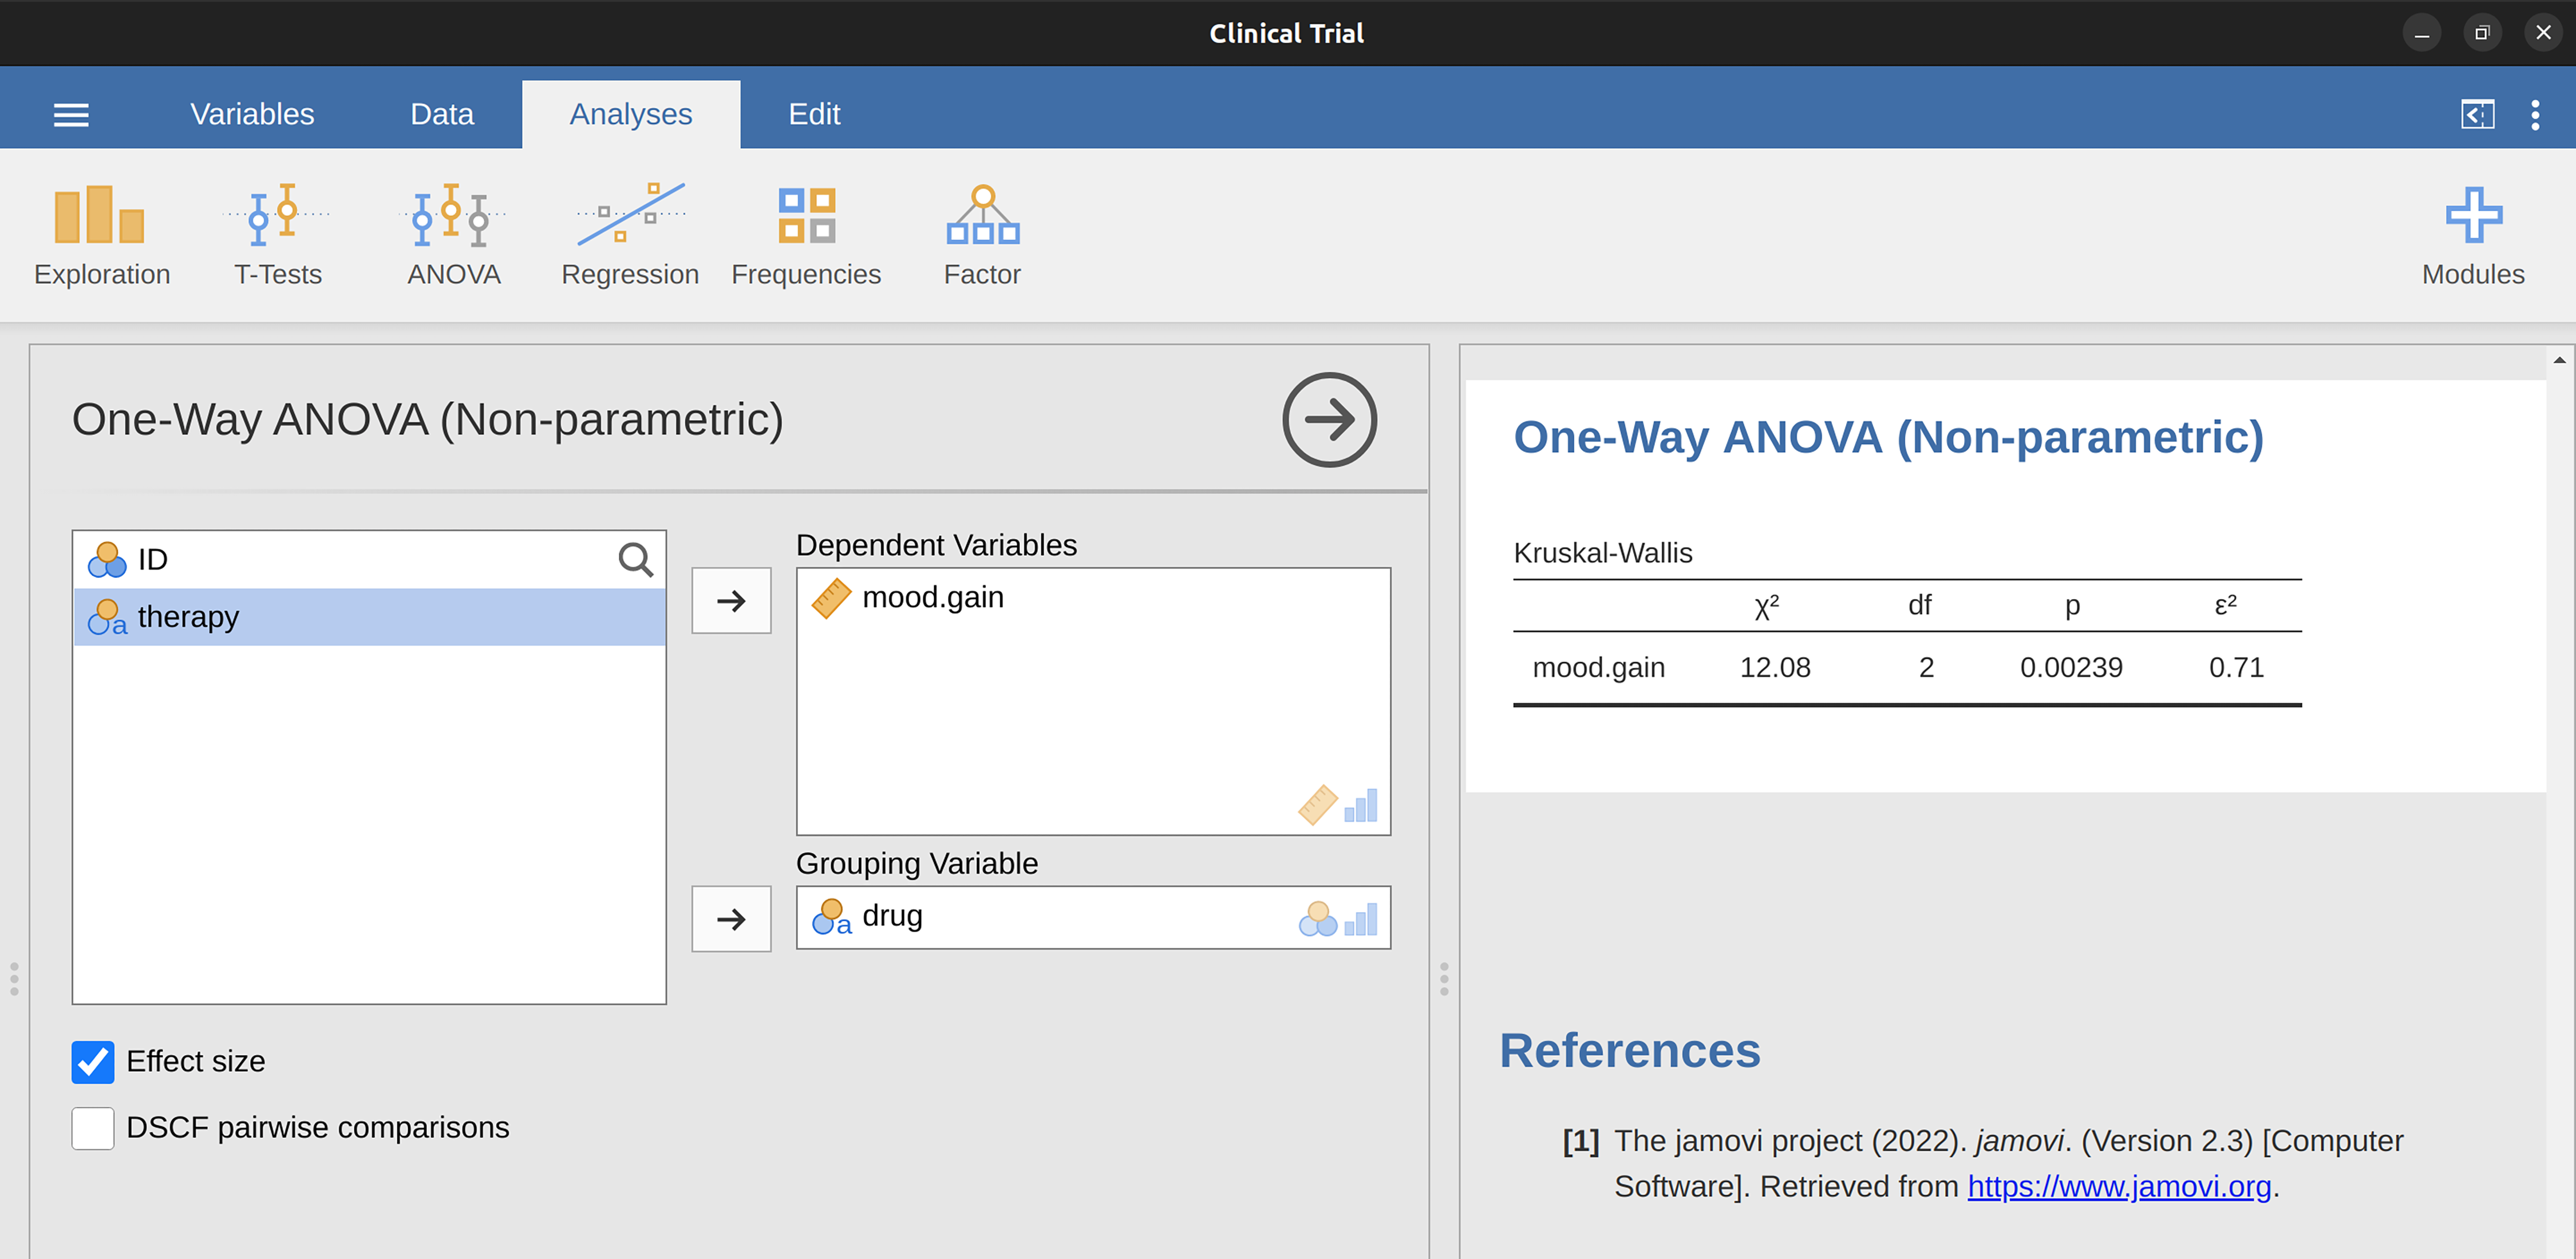
\includegraphics[width=1\textwidth,height=\textheight]{images/fig13-8.png} \hfill{}

\caption{\label{fig-fig13-8}Kruskal-Wallis one-way non-parametric ANOVA
in jamovi}

\end{figure}

\hypertarget{repeated-measures-one-way-anova}{%
\section{Repeated measures one-way
ANOVA}\label{repeated-measures-one-way-anova}}

The one-way repeated measures ANOVA test is a statistical method of
testing for significant differences between three or more groups where
the same participants are used in each group (or each participant is
closely matched with participants in other experimental groups). For
this reason, there should always be an equal number of scores (data
points) in each experimental group. This type of design and analysis can
also be called a ``related ANOVA'' or a ``within subjects ANOVA''.

The logic behind a repeated measures ANOVA is very similar to that of an
independent ANOVA (sometimes called a ``between subjects'' ANOVA).
You'll remember that earlier we showed that in a between subjects ANOVA
total variability is partitioned into between groups variability
(\(SS_b\)) and within groups variability (\(SS_w\)), and after each is
divided by the respective degrees of freedom to give \(MS_b\) and
\(MS_w\) (see Table 13.1) the \(F\)-ratio is calculated as:
\[F=\frac{MS_b}{MS_w}\]

In a repeated measures ANOVA, the \(F\)-ratio is calculated in a similar
way, but whereas in an independent ANOVA the within-group variability
(\(SS_w\)) is used as the basis for the \(MS_w\) denominator, in a
repeated measures ANOVA the \(SS_w\) is partioned into two parts. As we
are using the same subjects in each group, we can remove the variability
due to the individual differences between subjects (referred to as
\(SS_{subjects}\)) from the within groups variability. We won't go into
too much technical detail about how this is done, but essentially each
subject becomes a level of a factor called subjects. The variability in
this within subjects factor is then calculated in the same way as any
between subjects factor. And then we can subtract \(SS_{subjects}\))
from \(SS_w\) to provide a smaller \(SS_{error}\)) term:
\[\text{Independent ANOVA: } SS_{error} = SS_w\]
\[\text{Repeated Measures ANOVA: } SS_{error} = SS_w - SS_{subjects}\]
This change in \(SS_{error}\) term often leads to a more powerful
statistical test, but this does depend on whether the reduction in the
\(SS_{error}\) more than compensates for the reduction in degrees of
freedom for the error term (as degrees of freedom go from
\((n - k)\)\footnote{\((n - k)\): (number of subjects - number of
  groups)} to \((n - 1)(k - 1)\) (remembering that there are more
subjects in the independent ANOVA design).

\hypertarget{repeated-measures-anova-in-jamovi}{%
\subsection{Repeated measures ANOVA in
jamovi}\label{repeated-measures-anova-in-jamovi}}

First, we need some data. Geschwind (1972) has suggested that the exact
nature of a patient's language deficit following a stroke can be used to
diagnose the specific region of the brain that has been damaged. A
researcher is concerned with identifying the specific communication
difficulties experienced by six patients suffering from Broca's Aphasia
(a language deficit commonly experienced following a stroke)
(Table~\ref{tbl-tab13-12}).

\hypertarget{tbl-tab13-12}{}
 
  \providecommand{\huxb}[2]{\arrayrulecolor[RGB]{#1}\global\arrayrulewidth=#2pt}
  \providecommand{\huxvb}[2]{\color[RGB]{#1}\vrule width #2pt}
  \providecommand{\huxtpad}[1]{\rule{0pt}{#1}}
  \providecommand{\huxbpad}[1]{\rule[-#1]{0pt}{#1}}

\begin{table}[ht]
\caption{\label{tbl-tab13-12}Word recognition task scores in stroke patients }\tabularnewline

\begin{centerbox}
\begin{threeparttable}
\setlength{\tabcolsep}{0pt}
\begin{tabularx}{0.9\textwidth}{p{0.225\textwidth} p{0.225\textwidth} p{0.225\textwidth} p{0.225\textwidth}}


\hhline{>{\huxb{0, 0, 0}{0.4}}->{\huxb{0, 0, 0}{0.4}}->{\huxb{0, 0, 0}{0.4}}->{\huxb{0, 0, 0}{0.4}}-}
\arrayrulecolor{black}

\multicolumn{1}{!{\huxvb{0, 0, 0}{0}}p{0.225\textwidth}!{\huxvb{0, 0, 0}{0}}}{\hspace{0pt}\parbox[b]{0.225\textwidth-0pt-12pt}{\huxtpad{2pt + 1em}\centering \textbf{Participant}\huxbpad{2pt}}} &
\multicolumn{1}{p{0.225\textwidth}!{\huxvb{0, 0, 0}{0}}}{\hspace{12pt}\parbox[b]{0.225\textwidth-12pt-12pt}{\huxtpad{2pt + 1em}\centering \textbf{Speech}\huxbpad{2pt}}} &
\multicolumn{1}{p{0.225\textwidth}!{\huxvb{0, 0, 0}{0}}}{\hspace{12pt}\parbox[b]{0.225\textwidth-12pt-12pt}{\huxtpad{2pt + 1em}\centering \textbf{Conceptual}\huxbpad{2pt}}} &
\multicolumn{1}{p{0.225\textwidth}!{\huxvb{0, 0, 0}{0}}}{\hspace{12pt}\parbox[b]{0.225\textwidth-12pt-0pt}{\huxtpad{2pt + 1em}\centering \textbf{Syntax}\huxbpad{2pt}}} \tabularnewline[-0.5pt]


\hhline{>{\huxb{0, 0, 0}{0.4}}->{\huxb{0, 0, 0}{0.4}}->{\huxb{0, 0, 0}{0.4}}->{\huxb{0, 0, 0}{0.4}}-}
\arrayrulecolor{black}

\multicolumn{1}{!{\huxvb{0, 0, 0}{0}}p{0.225\textwidth}!{\huxvb{0, 0, 0}{0}}}{\hspace{0pt}\parbox[b]{0.225\textwidth-0pt-12pt}{\huxtpad{2pt + 1em}\centering 1\huxbpad{2pt}}} &
\multicolumn{1}{p{0.225\textwidth}!{\huxvb{0, 0, 0}{0}}}{\hspace{12pt}\parbox[b]{0.225\textwidth-12pt-12pt}{\huxtpad{2pt + 1em}\centering 8\huxbpad{2pt}}} &
\multicolumn{1}{p{0.225\textwidth}!{\huxvb{0, 0, 0}{0}}}{\hspace{12pt}\parbox[b]{0.225\textwidth-12pt-12pt}{\huxtpad{2pt + 1em}\centering 7\huxbpad{2pt}}} &
\multicolumn{1}{p{0.225\textwidth}!{\huxvb{0, 0, 0}{0}}}{\hspace{12pt}\parbox[b]{0.225\textwidth-12pt-0pt}{\huxtpad{2pt + 1em}\centering 6\huxbpad{2pt}}} \tabularnewline[-0.5pt]


\hhline{}
\arrayrulecolor{black}

\multicolumn{1}{!{\huxvb{0, 0, 0}{0}}p{0.225\textwidth}!{\huxvb{0, 0, 0}{0}}}{\hspace{0pt}\parbox[b]{0.225\textwidth-0pt-12pt}{\huxtpad{2pt + 1em}\centering 2\huxbpad{2pt}}} &
\multicolumn{1}{p{0.225\textwidth}!{\huxvb{0, 0, 0}{0}}}{\hspace{12pt}\parbox[b]{0.225\textwidth-12pt-12pt}{\huxtpad{2pt + 1em}\centering 7\huxbpad{2pt}}} &
\multicolumn{1}{p{0.225\textwidth}!{\huxvb{0, 0, 0}{0}}}{\hspace{12pt}\parbox[b]{0.225\textwidth-12pt-12pt}{\huxtpad{2pt + 1em}\centering 8\huxbpad{2pt}}} &
\multicolumn{1}{p{0.225\textwidth}!{\huxvb{0, 0, 0}{0}}}{\hspace{12pt}\parbox[b]{0.225\textwidth-12pt-0pt}{\huxtpad{2pt + 1em}\centering 6\huxbpad{2pt}}} \tabularnewline[-0.5pt]


\hhline{}
\arrayrulecolor{black}

\multicolumn{1}{!{\huxvb{0, 0, 0}{0}}p{0.225\textwidth}!{\huxvb{0, 0, 0}{0}}}{\hspace{0pt}\parbox[b]{0.225\textwidth-0pt-12pt}{\huxtpad{2pt + 1em}\centering 3\huxbpad{2pt}}} &
\multicolumn{1}{p{0.225\textwidth}!{\huxvb{0, 0, 0}{0}}}{\hspace{12pt}\parbox[b]{0.225\textwidth-12pt-12pt}{\huxtpad{2pt + 1em}\centering 9\huxbpad{2pt}}} &
\multicolumn{1}{p{0.225\textwidth}!{\huxvb{0, 0, 0}{0}}}{\hspace{12pt}\parbox[b]{0.225\textwidth-12pt-12pt}{\huxtpad{2pt + 1em}\centering 5\huxbpad{2pt}}} &
\multicolumn{1}{p{0.225\textwidth}!{\huxvb{0, 0, 0}{0}}}{\hspace{12pt}\parbox[b]{0.225\textwidth-12pt-0pt}{\huxtpad{2pt + 1em}\centering 3\huxbpad{2pt}}} \tabularnewline[-0.5pt]


\hhline{}
\arrayrulecolor{black}

\multicolumn{1}{!{\huxvb{0, 0, 0}{0}}p{0.225\textwidth}!{\huxvb{0, 0, 0}{0}}}{\hspace{0pt}\parbox[b]{0.225\textwidth-0pt-12pt}{\huxtpad{2pt + 1em}\centering 4\huxbpad{2pt}}} &
\multicolumn{1}{p{0.225\textwidth}!{\huxvb{0, 0, 0}{0}}}{\hspace{12pt}\parbox[b]{0.225\textwidth-12pt-12pt}{\huxtpad{2pt + 1em}\centering 5\huxbpad{2pt}}} &
\multicolumn{1}{p{0.225\textwidth}!{\huxvb{0, 0, 0}{0}}}{\hspace{12pt}\parbox[b]{0.225\textwidth-12pt-12pt}{\huxtpad{2pt + 1em}\centering 4\huxbpad{2pt}}} &
\multicolumn{1}{p{0.225\textwidth}!{\huxvb{0, 0, 0}{0}}}{\hspace{12pt}\parbox[b]{0.225\textwidth-12pt-0pt}{\huxtpad{2pt + 1em}\centering 5\huxbpad{2pt}}} \tabularnewline[-0.5pt]


\hhline{}
\arrayrulecolor{black}

\multicolumn{1}{!{\huxvb{0, 0, 0}{0}}p{0.225\textwidth}!{\huxvb{0, 0, 0}{0}}}{\hspace{0pt}\parbox[b]{0.225\textwidth-0pt-12pt}{\huxtpad{2pt + 1em}\centering 5\huxbpad{2pt}}} &
\multicolumn{1}{p{0.225\textwidth}!{\huxvb{0, 0, 0}{0}}}{\hspace{12pt}\parbox[b]{0.225\textwidth-12pt-12pt}{\huxtpad{2pt + 1em}\centering 6\huxbpad{2pt}}} &
\multicolumn{1}{p{0.225\textwidth}!{\huxvb{0, 0, 0}{0}}}{\hspace{12pt}\parbox[b]{0.225\textwidth-12pt-12pt}{\huxtpad{2pt + 1em}\centering 6\huxbpad{2pt}}} &
\multicolumn{1}{p{0.225\textwidth}!{\huxvb{0, 0, 0}{0}}}{\hspace{12pt}\parbox[b]{0.225\textwidth-12pt-0pt}{\huxtpad{2pt + 1em}\centering 2\huxbpad{2pt}}} \tabularnewline[-0.5pt]


\hhline{}
\arrayrulecolor{black}

\multicolumn{1}{!{\huxvb{0, 0, 0}{0}}p{0.225\textwidth}!{\huxvb{0, 0, 0}{0}}}{\hspace{0pt}\parbox[b]{0.225\textwidth-0pt-12pt}{\huxtpad{2pt + 1em}\centering 6\huxbpad{2pt}}} &
\multicolumn{1}{p{0.225\textwidth}!{\huxvb{0, 0, 0}{0}}}{\hspace{12pt}\parbox[b]{0.225\textwidth-12pt-12pt}{\huxtpad{2pt + 1em}\centering 8\huxbpad{2pt}}} &
\multicolumn{1}{p{0.225\textwidth}!{\huxvb{0, 0, 0}{0}}}{\hspace{12pt}\parbox[b]{0.225\textwidth-12pt-12pt}{\huxtpad{2pt + 1em}\centering 7\huxbpad{2pt}}} &
\multicolumn{1}{p{0.225\textwidth}!{\huxvb{0, 0, 0}{0}}}{\hspace{12pt}\parbox[b]{0.225\textwidth-12pt-0pt}{\huxtpad{2pt + 1em}\centering 4\huxbpad{2pt}}} \tabularnewline[-0.5pt]


\hhline{>{\huxb{0, 0, 0}{0.4}}->{\huxb{0, 0, 0}{0.4}}->{\huxb{0, 0, 0}{0.4}}->{\huxb{0, 0, 0}{0.4}}-}
\arrayrulecolor{black}
\end{tabularx} 

\end{threeparttable}\par\end{centerbox}

\end{table}
 

The patients were required to complete three word recognition tasks. On
the first (speech production) task, patients were required to repeat
single words read out aloud by the researcher. On the second
(conceptual) task, designed to test word comprehension, patients were
required to match a series of pictures with their correct name. On the
third (syntax) task, designed to test knowledge of correct word order,
patients were asked to reorder syntactically incorrect sentences. Each
patient completed all three tasks. The order in which patients attempted
the tasks was counterbalanced between participants. Each task consisted
of a series of 10 attempts. The number of attempts successfully
completed by each patient are shown in Table~\ref{tbl-tab13-11}. Enter
these data into jamovi ready for analysis (or take a short-cut and load
up the \emph{broca.csv} file).

To perform a one-way related ANOVA in jamovi, open the one-way repeated
measures ANOVA dialogue box, as in Figure~\ref{fig-fig13-9}, via ANOVA -
Repeated Measures ANOVA.

\begin{figure}

{\centering 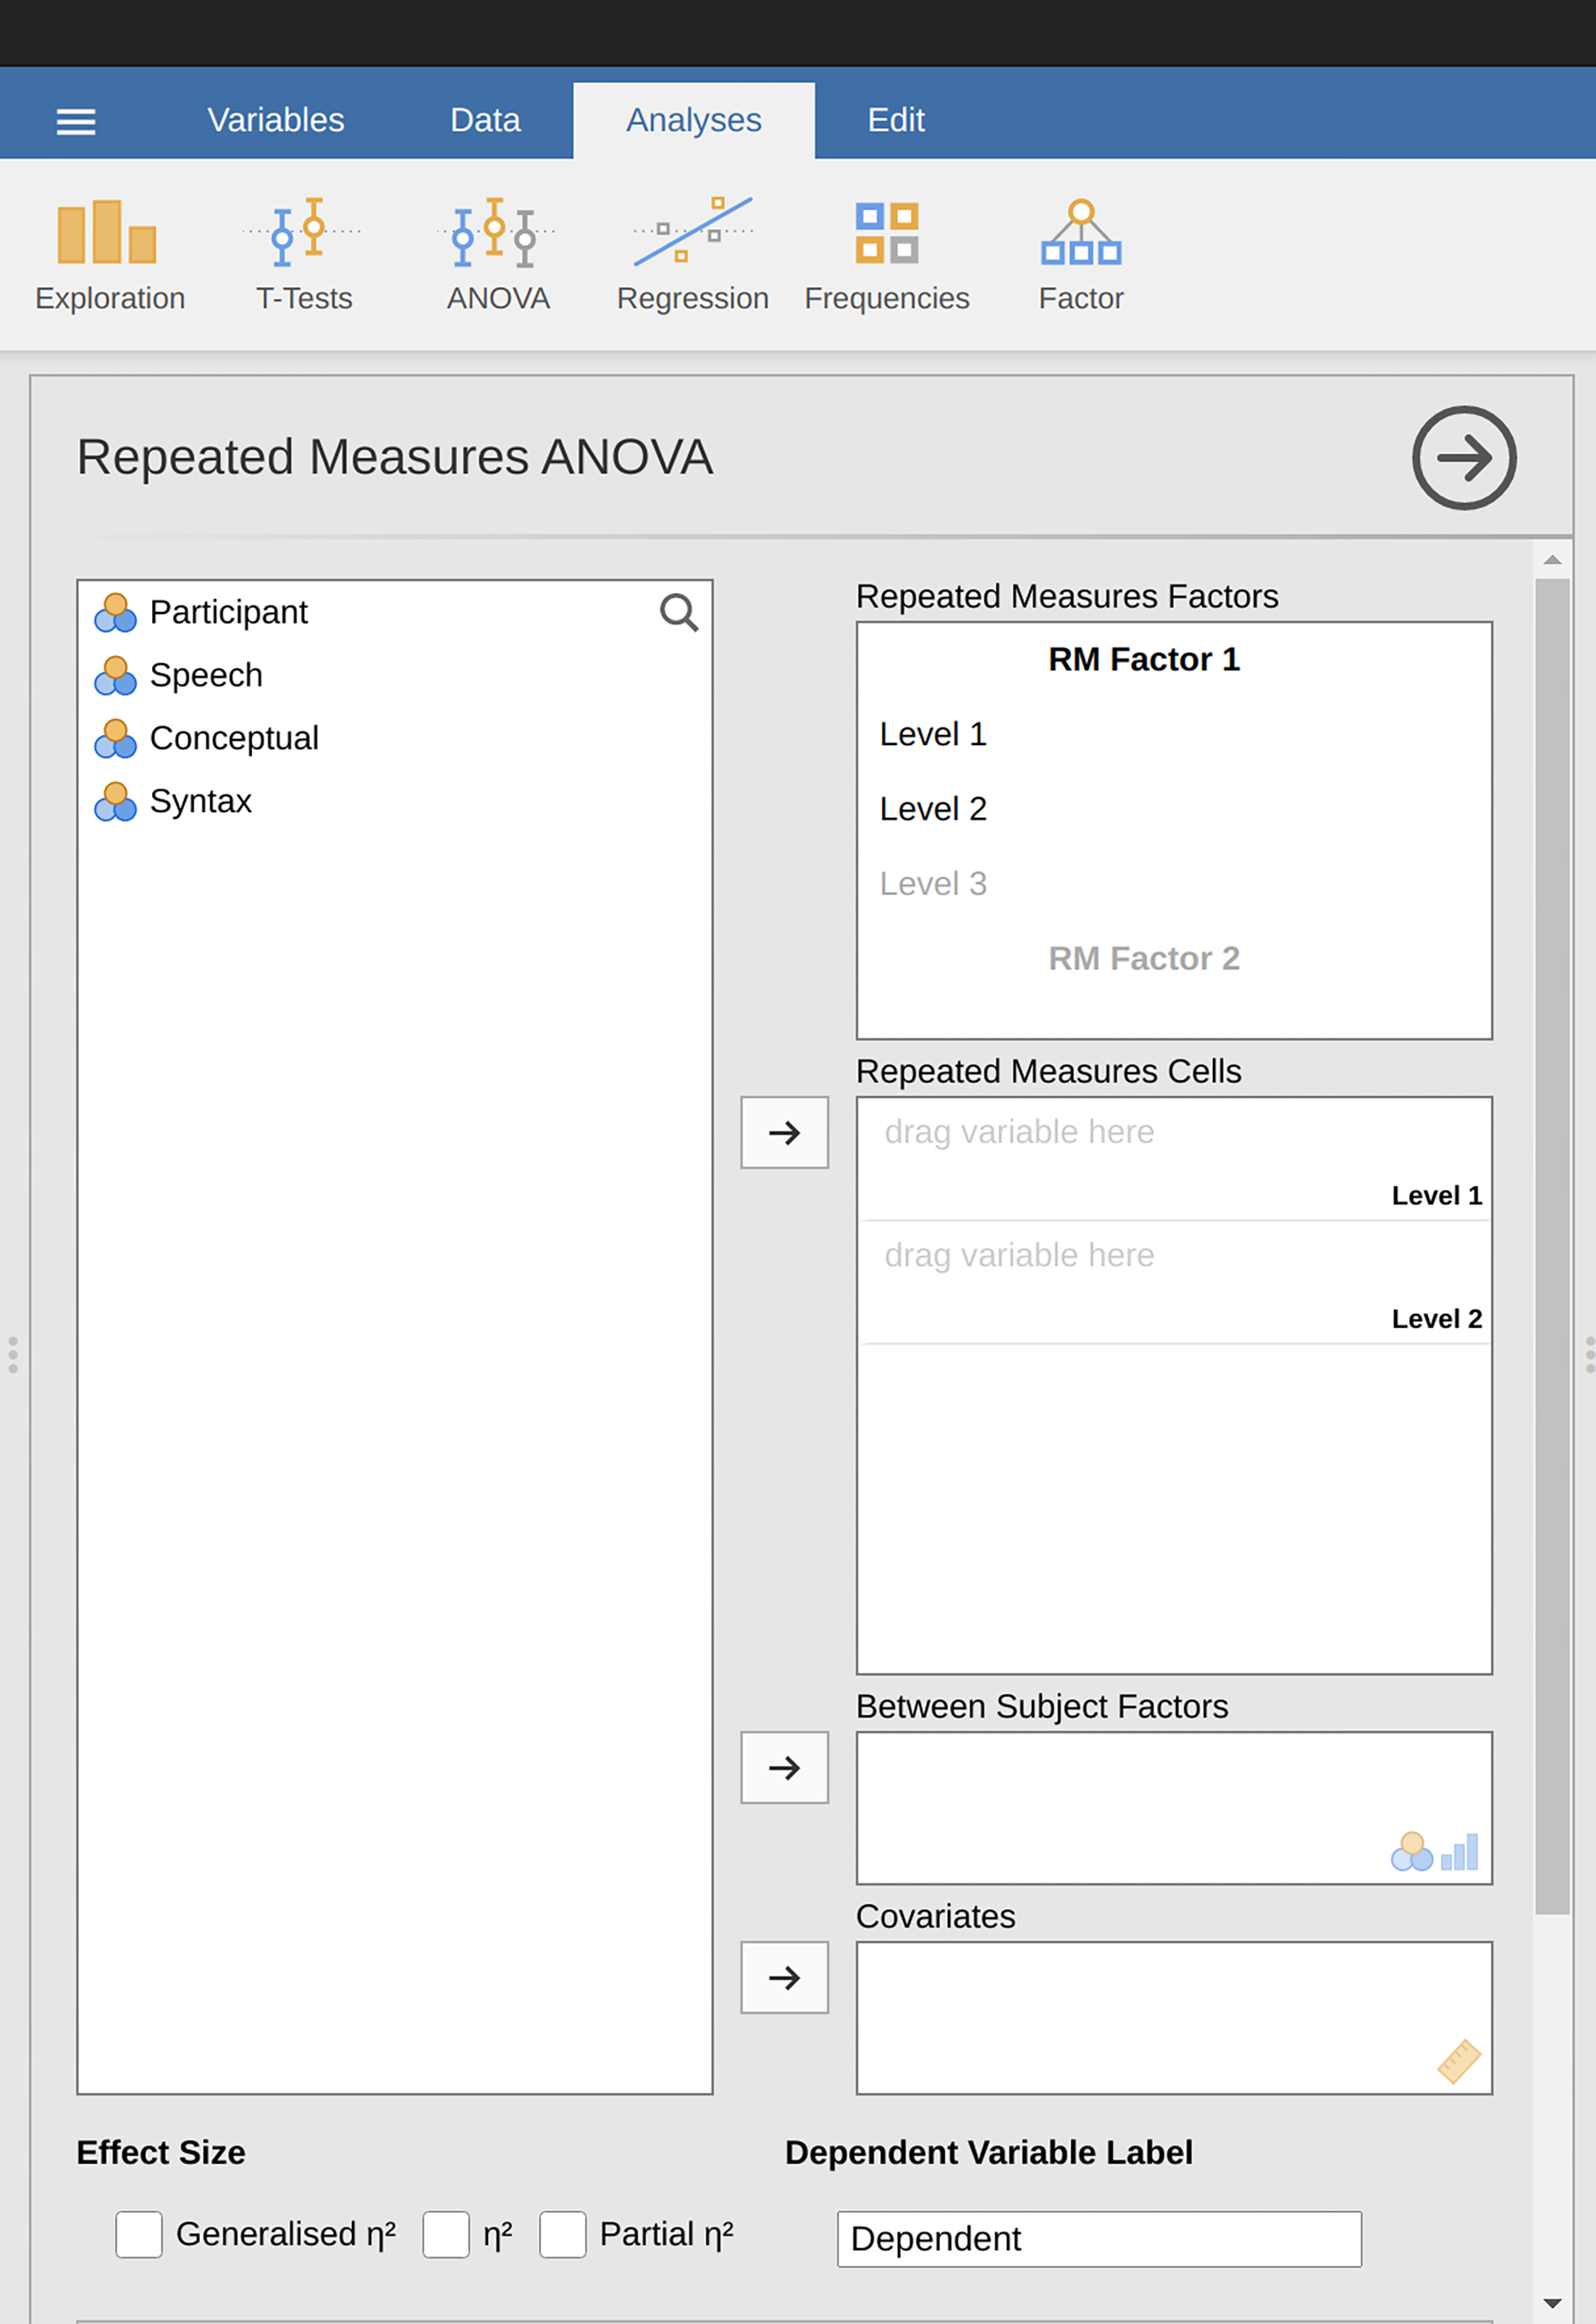
\includegraphics[width=0.8\textwidth,height=\textheight]{images/fig13-9.png}

}

\caption{\label{fig-fig13-9}Repeated measures ANOVA dialogue box in
jamovi}

\end{figure}

Then:

\begin{itemize}
\tightlist
\item
  Enter a `Repeated Measures' factor name. This should be a label that
  you choose to describe the conditions repeated by all participants.
  For example, to describe the speech, conceptual and syntax tasks
  completed by all participants a suitable label would be `Task'. Note
  that this new factor name represents the independent variable in the
  analysis.
\item
  Add a third level in the `Repeated Measures Factors' text box, as
  there are three levels representing the three tasks: speech,
  conceptual and syntax. Change the labels of the levels accordingly.
\item
  Then move each of the levels variables across to the `Repeated
  Measures' Cells text box.
\item
  Finally, under the `Assumption Checks' option, tick the `Sphericity
  checks' text box.
\end{itemize}

jamovi output for a one-way repeated measures ANOVA is produced as shown
in Figure~\ref{fig-fig13-10} to Figure~\ref{fig-fig13-13}. The first
output we should look at is Mauchly's Test of Sphericity, which tests
the hypothesis that the variances of the differences between the
conditions are equal (meaning that the spread of difference scores
between the study conditions is approximately the same). In
Figure~\ref{fig-fig13-10} the significance level in Mauchly's test is
\(p = .720\). If Mauchly's test is non-significant (i.e.~\(p > .05\), as
is the case in this analysis) then it is reasonable to conclude that the
variances of the differences are not significantly different (i.e.~they
are roughly equal and sphericity can be assumed).

\begin{figure}

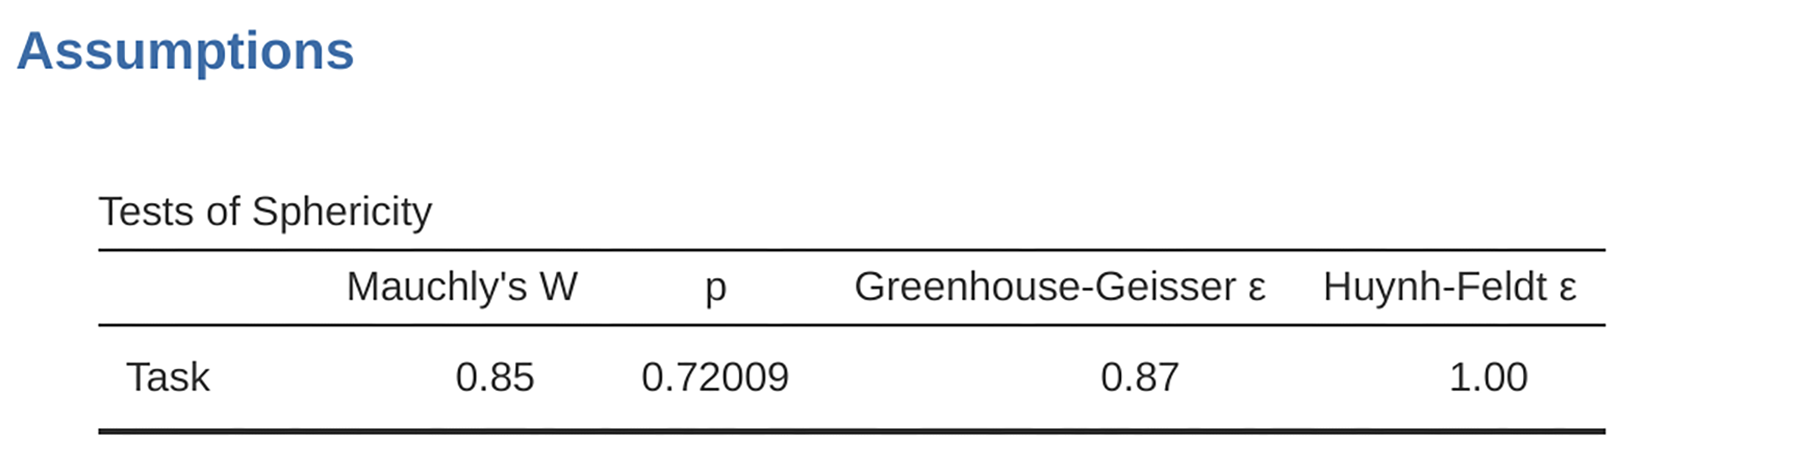
\includegraphics[width=1\textwidth,height=\textheight]{images/fig13-10.png} \hfill{}

\caption{\label{fig-fig13-10}One-way repeated measures ANOVA output --
Mauchly Test of Sphericity}

\end{figure}

If, on the other hand, Mauchly's test had been significant (\(p\)
\textless{} .05) then we would conclude that there are significant
differences between the variance of the differences, and the requirement
of sphericity has not been met. In this case, we should apply a
correction to the \(F\)-value obtained in the one-way related ANOVA
analysis:

\begin{itemize}
\tightlist
\item
  If the Greenhouse-Geisser value in the ``Tests of Sphericity'' table
  is \textgreater{} .75 then you should use the Huynh-Feldt correction
\item
  But if the Greenhouse-Geisser value is \textless{} .75, then you
  should use the Greenhouse-Geisser correction.
\end{itemize}

Both these corrected \(F\)-values can be specified in the `Sphericity
Corrections' check boxes under the `Assumption Checks' options, and the
corrected \(F\)-values are then shown in the results table, as in Figure
\textbf{13.11}.

\begin{figure}

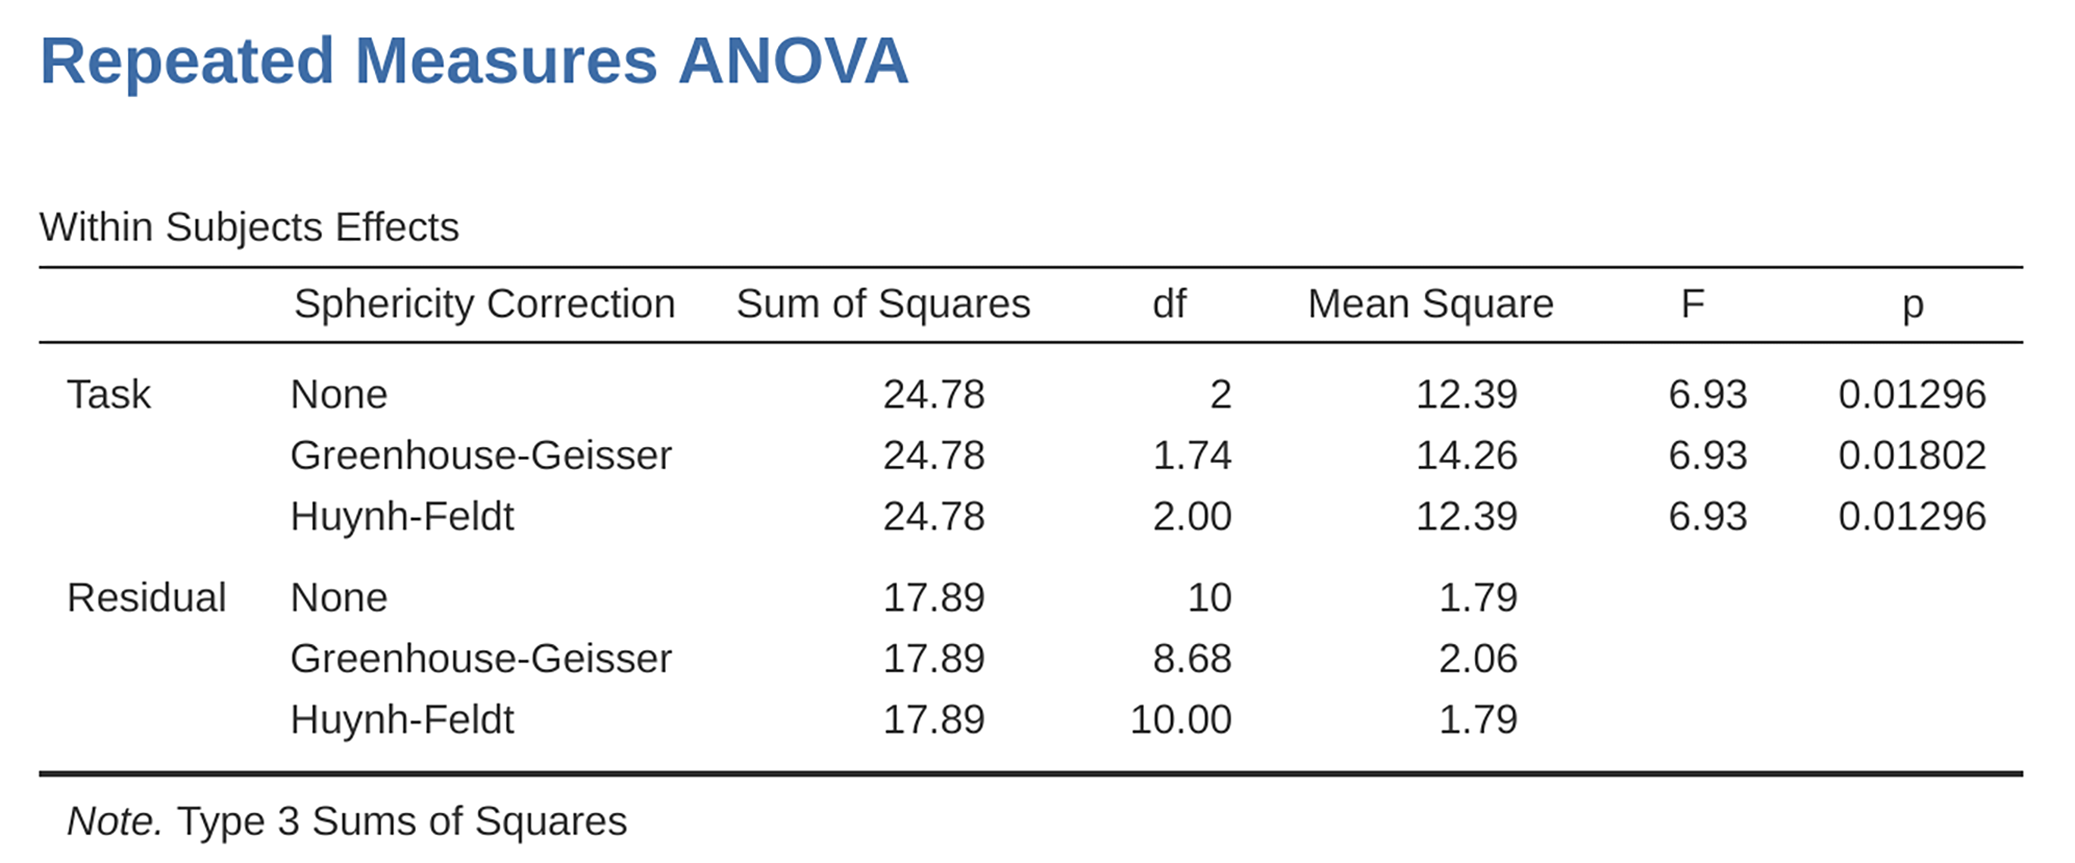
\includegraphics[width=1\textwidth,height=\textheight]{images/fig13-11.png} \hfill{}

\caption{\label{fig-fig13-11}One-way repeated measures ANOVA output --
Tests of Within Subjects Effects}

\end{figure}

In our analysis, we saw that the significance of Mauchly's Test of
Sphericity was \(p = .720\) (i.e., \(p > 0.05)\). So, this means we can
assume that the requirement of sphericity has been met so no correction
to the \(F\)-value is needed. Therefore, we can use the `None'
Sphericity Correction output values for the repeated measure `Task':
\(F = 6.93\), \(df = 2\), \(p = .013\), and we can conclude that the
number of tests successfully completed on each language task did vary
significantly depending on whether the task was speech, comprehension or
syntax based (\(F(2, 10) = 6.93\), \(p = .013\)).

Post hoc tests can also be specified in jamovi for repeated measures
ANOVA in the same way as for independent ANOVA. The results are shown in
Figure~\ref{fig-fig13-12}. These indicate that there is a significant
difference between Speech and Syntax, but not between other levels.

\begin{figure}

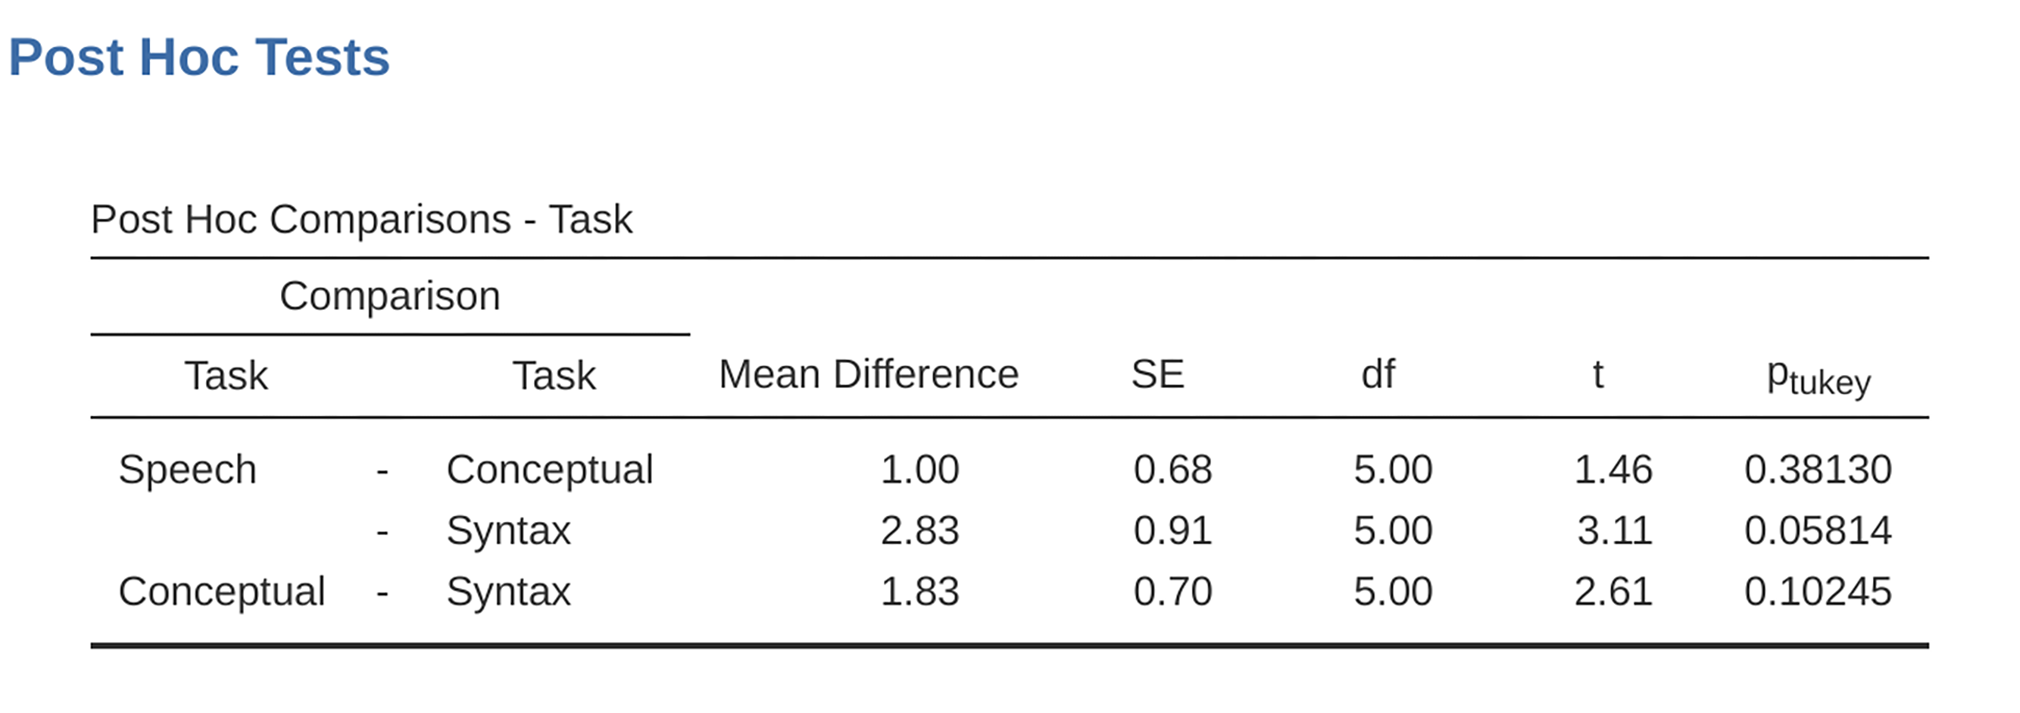
\includegraphics[width=1\textwidth,height=\textheight]{images/fig13-12.png} \hfill{}

\caption{\label{fig-fig13-12}Post hoc tests in repeated measures ANOVA
in jamovi}

\end{figure}

Descriptive statistics (marginal means) can be reviewed to help
interpret the results, produced in the jamovi output as in
Figure~\ref{fig-fig13-13}. Comparison of the mean number of trials
successfully completed by participants shows that Broca's Aphasics
perform reasonably well on speech production (mean = 7.17) and language
comprehension (mean = 6.17) tasks. However, their performance was
considerably worse on the syntax task (mean = 4.33), with a significant
difference in post hoc tests between Speech and Syntax task performance.

\begin{figure}

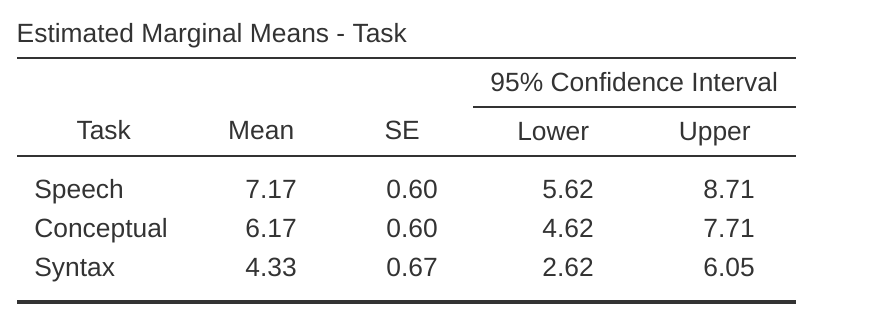
\includegraphics[width=1\textwidth,height=\textheight]{images/fig13-13.png} \hfill{}

\caption{\label{fig-fig13-13}One-way repeated measures ANOVA output --
Descriptive Statistics}

\end{figure}

\hypertarget{the-friedman-non-parametric-repeated-measures-anova-test}{%
\section{The Friedman non-parametric repeated measures ANOVA
test}\label{the-friedman-non-parametric-repeated-measures-anova-test}}

The Friedman test is a non-parametric version of a repeated measures
ANOVA and can be used instead of the Kruskal-Wallis test when testing
for differences between three or more groups where the same participants
are in each group, or each participant is closely matched with
participants in other conditions. If the dependent variable is ordinal,
or if the assumption of normality is not met, then the Friedman test can
be used.

As with the Kruskal-Wallis test, the underlying mathematics is
complicated, and won't be presented here. For the purpose of this book,
it is sufficient to note that jamovi calculates the tie-corrected
version of the Friedman test, and in Figure~\ref{fig-fig13-14} there is
an example using the Broca's Aphasia data we have already looked at.

\begin{figure}

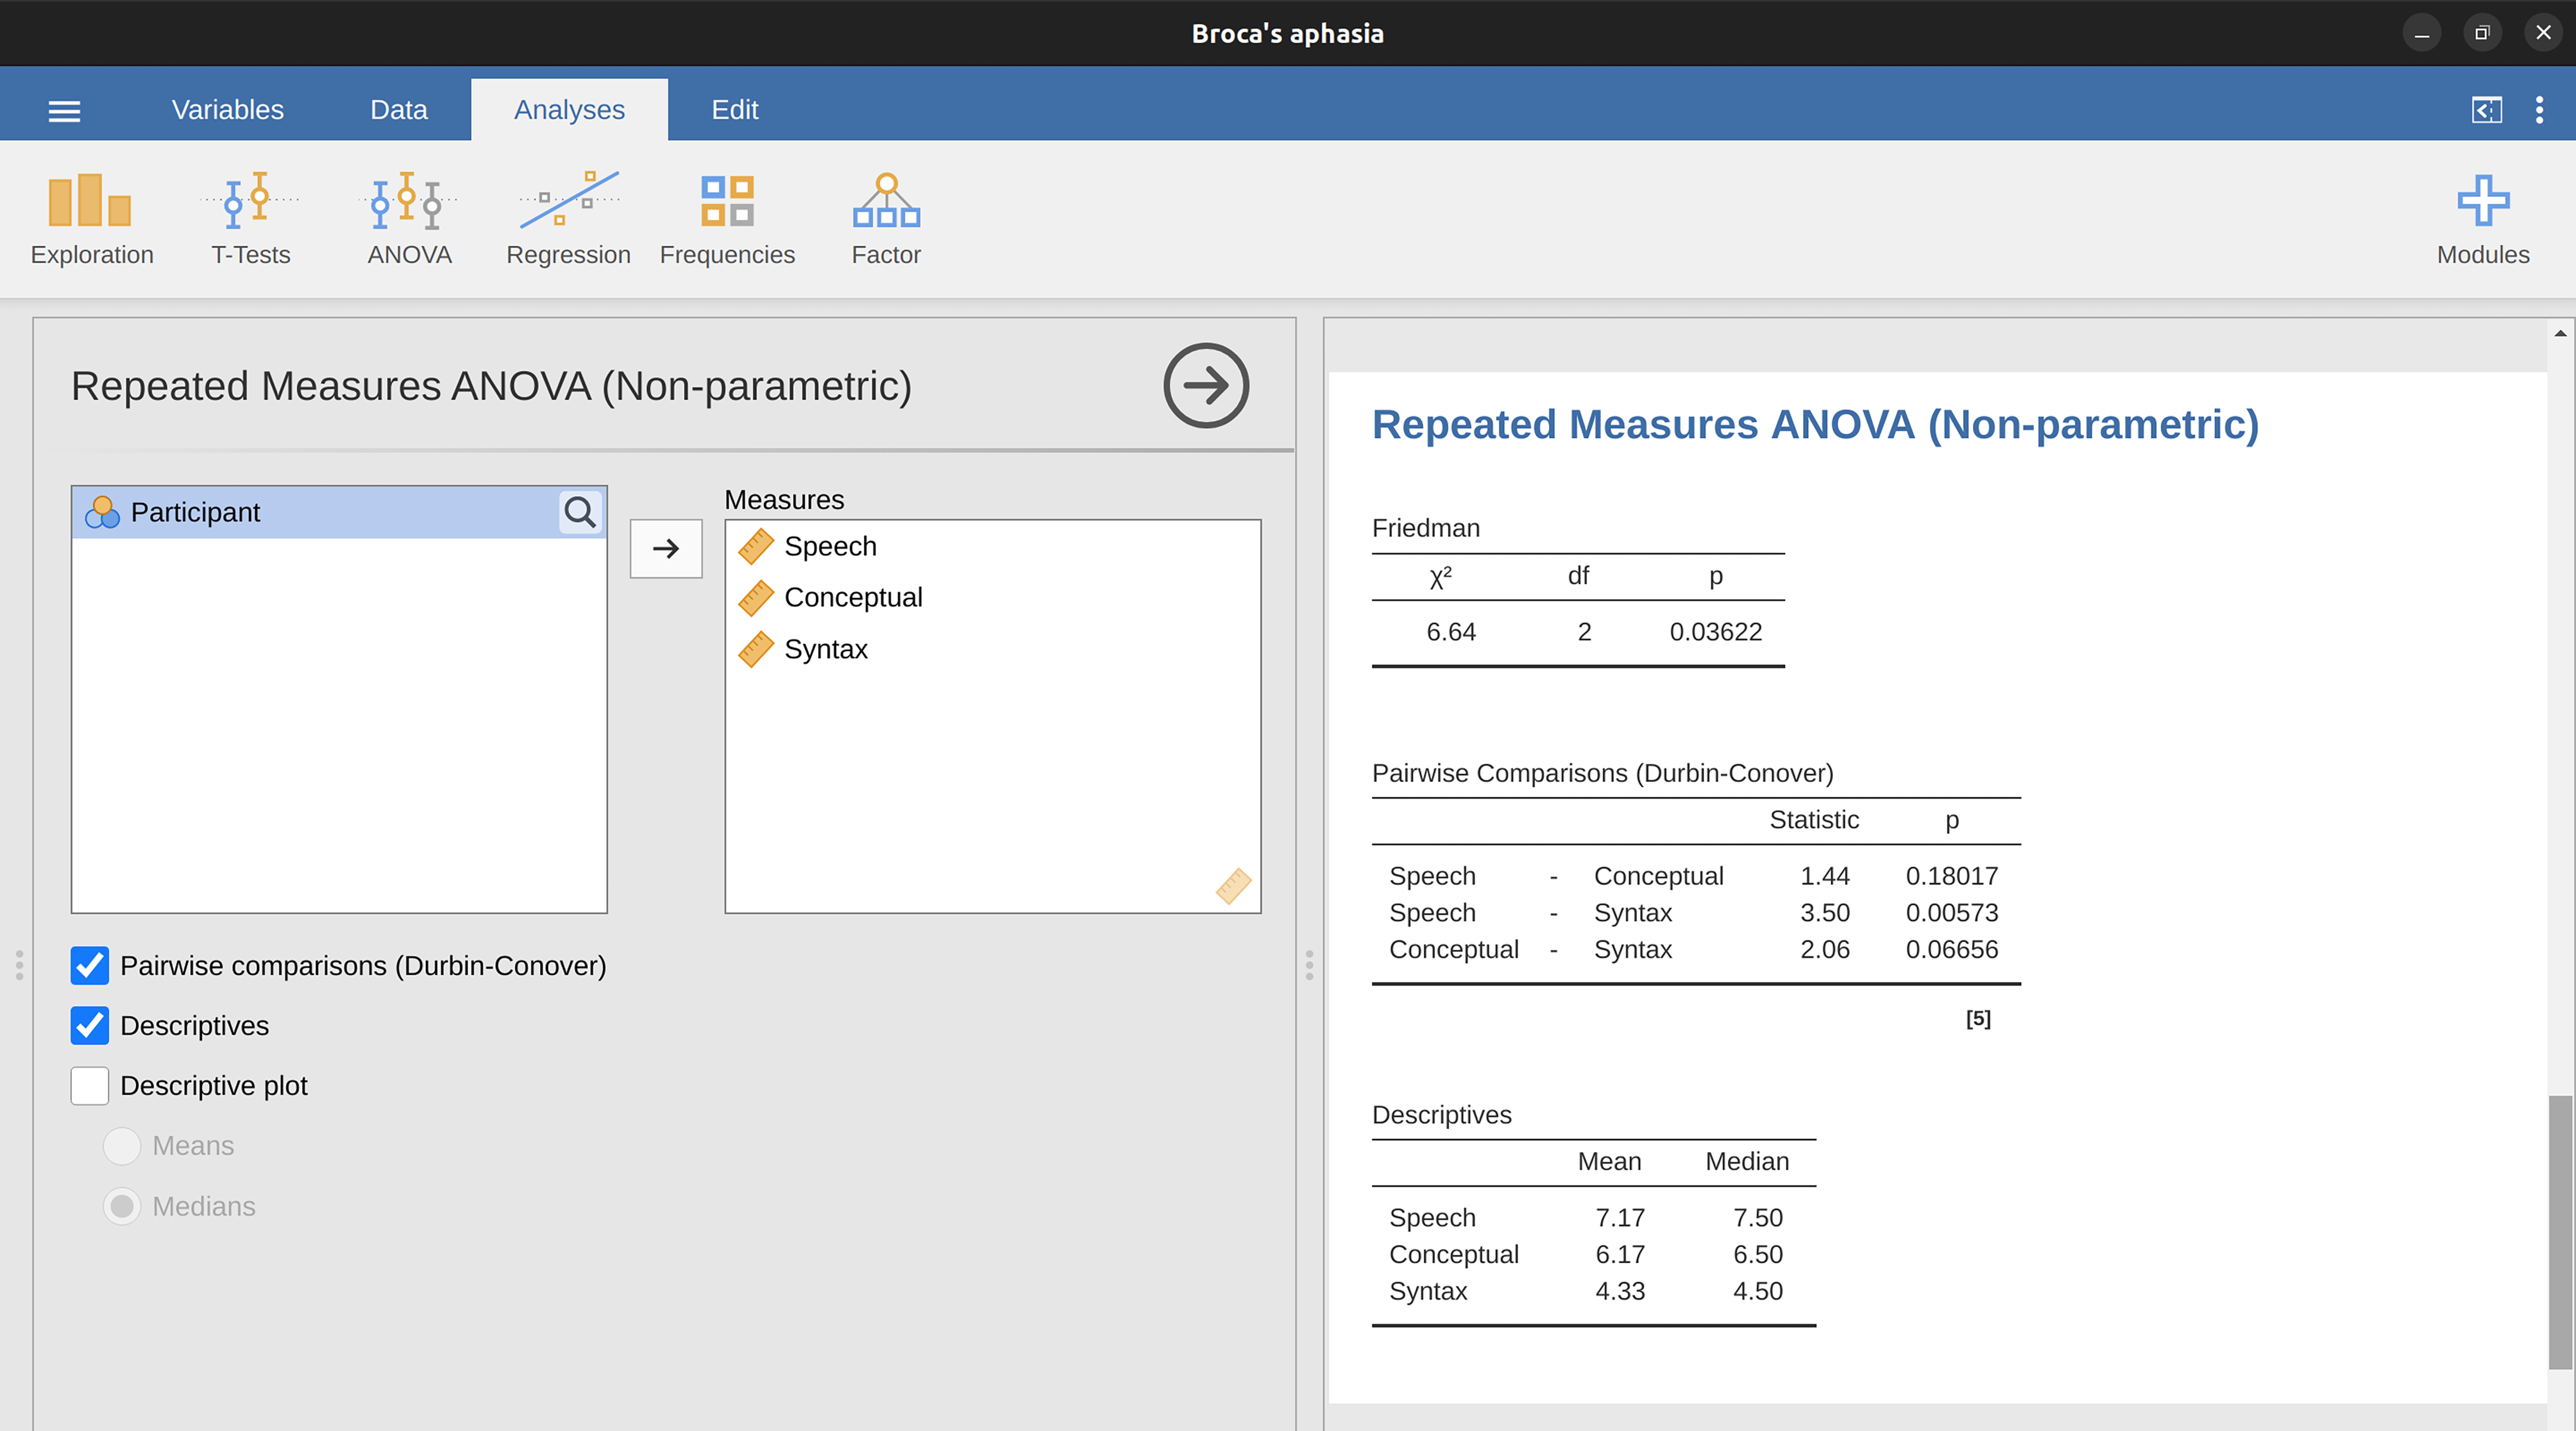
\includegraphics[width=1\textwidth,height=\textheight]{images/fig13-14.png} \hfill{}

\caption{\label{fig-fig13-14}The `Repeated Measures ANOVA
(Non-parametric)' dialogue box and results in jamovi}

\end{figure}

It's pretty straightforward to run a Friedman test in jamovi. Just
select `Analyses - ANOVA - Repeated Measures ANOVA (Non-parametric)' as
in Figure~\ref{fig-fig13-14}. Then highlight and transfer the names of
the repeated measures variables you wish to compare (Speech, Conceptual,
Syntax) into the `Measures:' text box. To produce descriptive statistics
(means and medians) for the three repeated measures variables, click on
the `Descriptives' button.

The jamovi results show descriptive statistics, chi-square value,
degrees of freedom, and the \(p\)-value (Figure~\ref{fig-fig13-14}).
Since the \(p\)-value is less than the level conventionally used to
determine significance (\(p < .05\)), we can conclude that Broca's
Aphasics perform reasonably well on speech production (median = 7.5) and
language comprehension (median = 6.5) tasks. However, their performance
was considerably worse on the syntax task (median = 4.5), with a
significant difference in post hoc tests between Speech and Syntax task
performance.

\hypertarget{sec-On-the-relationship-between-ANOVA-and-the-Student-t-test}{%
\section{\texorpdfstring{On the relationship between ANOVA and the
Student
\(t\)-test}{On the relationship between ANOVA and the Student t-test}}\label{sec-On-the-relationship-between-ANOVA-and-the-Student-t-test}}

There's one last thing I want to point out before finishing. It's
something that a lot of people find kind of surprising, but it's worth
knowing about. An ANOVA with two groups is identical to the Student
\(t\)-test. No, really. It's not just that they are similar, but they
are actually equivalent in every meaningful way. I won't try to prove
that this is always true, but I will show you a single concrete
demonstration. Suppose that, instead of running an ANOVA on our
mood.gain \textasciitilde{} drug model, let's instead do it using
therapy as the predictor. If we run this ANOVA we get an \(F\)-statistic
of \(F(1,16) = 1.71\), and a \(p\)-value = \(0.21\). Since we only have
two groups, I didn't actually need to resort to an ANOVA, I could have
just decided to run a Student \(t\)-test. So let's see what happens when
I do that: I get a \(t\)-statistic of \(t(16) = -1.3068\) and a
\(p\)-value = 0.21. Curiously, the \(p\)-values are identical. Once
again we obtain a value of \(p = .21\). But what about the test
statistic? Having run a \(t\)-test instead of an ANOVA, we get a
somewhat different answer, namely \(t(16) = -1.3068\). However, there is
a fairly straightforward relationship here. If we square the
\(t\)-statistic then we get the \(F\)-statistic from before:
\$-1.3068\^{}\{2\} = 1.7077\$4.

\hypertarget{summary}{%
\section{Summary}\label{summary}}

There's a fair bit covered in this chapter, but there's still a lot
missing\footnote{As with all of the chapters in this book, there are
  quite a few different sources that I've relied upon, but the one
  stand-out text that I've been most heavily influenced by is Sahai \&
  Ageel (2000). It's not a good book for beginners, but it's an
  excellent book for more advanced readers who are interested in
  understanding the mathematics behind ANOVA.}. Most obviously, I
haven't discussed how to run an ANOVA when you are interested in more
than one grouping variable, but that will be discussed in a lot of
detail in \textbf{?@sec-Factorial-ANOVA}. In terms of what we have
discussed, the key topics were:

\begin{itemize}
\tightlist
\item
  The basic logic behind \protect\hyperlink{sec-How-ANOVA-works}{How
  ANOVA works} and
  \protect\hyperlink{running-an-anova-in-jamovi}{Running an ANOVA in
  jamovi}.
\item
  How to compute an \protect\hyperlink{effect-size}{Effect size} for an
  ANOVA.
\item
  \protect\hyperlink{multiple-comparisons-and-post-hoc-tests}{Multiple
  comparisons and post hoc tests} for multiple testing.
\item
  \protect\hyperlink{the-assumptions-of-one-way-anova}{The assumptions
  of one-way ANOVA}.
\item
  \protect\hyperlink{sec-Checking-the-homogeneity-of-variance-assumption}{Checking
  the homogeneity of variance assumption} and what to do if it is
  violated:
  \protect\hyperlink{removing-the-homogeneity-of-variance-assumption}{Removing
  the homogeneity of variance assumption}.
\item
  \protect\hyperlink{sec-Checking-the-normality-assumption}{Checking the
  normality assumption} and what to do if it is violated:
  \protect\hyperlink{removing-the-normality-assumption}{Removing the
  normality assumption}.
\item
  \protect\hyperlink{repeated-measures-one-way-anova}{Repeated measures
  one-way ANOVA} and the non-parametric equivalent,
  \protect\hyperlink{the-friedman-non-parametric-repeated-measures-anova-test}{The
  Friedman non-parametric repeated measures ANOVA test}.
\end{itemize}

\part{Endings, alternatives and prospects}

\hypertarget{sec-Bayesian-statistics}{%
\chapter{Bayesian statistics}\label{sec-Bayesian-statistics}}

\placetextbox{0.26}{0.06}{\scriptsize{©2025 D. Foxcroft and D. Navarro,}}
\placetextbox{0.20}{0.05}{\scriptsize{CC BY-NC 4.0}}
\placetextbox{0.70}{0.06}{\scriptsize{\url{https://doi.org/10.11647/OBP.0333/16}}}

\begin{quote}
\emph{In our reasonings concerning matter of fact, there are all
imaginable degrees of assurance, from the highest certainty to the
lowest species of moral evidence. A wise man, therefore, proportions his
belief to the evidence.}\\
-- David Hume\footnote{\href{http://en.wikiquote.org/wiki/David_Hume}{http://en.wikiquote.org/wiki/David\%20Hume}.}
\end{quote}

The ideas I've presented to you in this book describe inferential
statistics from the frequentist perspective. I'm not alone in doing
this. In fact, almost every textbook given to undergraduate psychology
students presents the opinions of the frequentist statistician as
\emph{the} theory of inferential statistics, the one true way to do
things. I have taught this way for practical reasons. The frequentist
view of statistics dominated the academic field of statistics for most
of the 20th century, and this dominance is even more extreme among
applied scientists. It was and is current practice among psychologists
to use frequentist methods. Because frequentist methods are ubiquitous
in scientific papers, every student of statistics needs to understand
those methods, otherwise they will be unable to make sense of what those
papers are saying! Unfortunately, in my opinion at least, the current
practice in psychology is often misguided, and the reliance on
frequentist methods is partly to blame. In this chapter I explain why I
think this and provide an introduction to Bayesian statistics, an
approach that I think is generally superior to the orthodox approach.

This chapter comes in two parts. In the first three sections I talk
about what Bayesian statistics are all about, covering the basic
mathematical rules for how it works as well as an explanation for why I
think the Bayesian approach is so useful. Afterwards, I provide a brief
overview of how you can do \protect\hyperlink{bayesian-t-tests}{Bayesian
\(t\)-tests}.

\hypertarget{probabilistic-reasoning-by-rational-agents}{%
\section{Probabilistic reasoning by rational
agents}\label{probabilistic-reasoning-by-rational-agents}}

From a Bayesian perspective statistical inference is all about
\emph{belief revision}. I start out with a set of candidate hypotheses,
\(h\), about the world. I don't know which of these hypotheses is true,
but do I have some beliefs about which hypotheses are plausible and
which are not. When I observe the data, \(d\), I have to revise those
beliefs. If the data are consistent with a hypothesis, my belief in that
hypothesis is strengthened. If the data are inconsistent with the
hypothesis, my belief in that hypothesis is weakened. That's it! At the
end of this section I'll give a precise description of how Bayesian
reasoning works, but first I want to work through a simple example in
order to introduce the key ideas. Consider the following reasoning
problem:

\begin{quote}
\emph{I'm carrying an umbrella. Do you think it will rain?}
\end{quote}

In this problem I have presented you with a single piece of data (\(d\)
= I'm carrying the umbrella), and I'm asking you to tell me your belief
or hypothesis about whether it's raining. You have two alternatives,
\(h\): either it will rain today or it will not. How should you solve
this problem?

\hypertarget{priors-what-you-believed-before}{%
\subsection{Priors: what you believed
before}\label{priors-what-you-believed-before}}

The first thing you need to do is ignore what I told you about the
umbrella, and write down your pre-existing beliefs about rain. This is
important. If you want to be honest about how your beliefs have been
revised in the light of new evidence (data) then you must say something
about what you believed before those data appeared! So, what might you
believe about whether it will rain today? You probably know that I live
in Australia and that much of Australia is hot and dry. The city of
Adelaide where I live has a Mediterranean climate, very similar to
southern California, southern Europe or northern Africa. I'm writing
this in January and so you can assume it's the middle of summer. In
fact, you might have decided to take a quick look on
Wikipedia\footnote{\url{http://en.wikipedia.org/wiki/Climate_of_Adelaide}}
and discovered that Adelaide gets an average of 4.4 days of rain across
the 31 days of January. Without knowing anything else, you might
conclude that the probability of January rain in Adelaide is about 15\%,
and the probability of a dry day is 85\% (see Table~\ref{tbl-tab16-1}).
If this is really what you believe about Adelaide rainfall (and now that
I've told it to you I'm betting that this really is what you believe)
then what I have written here is your \textbf{prior distribution},
written \(P(h)\).

\hypertarget{tbl-tab16-1}{}
 
  \providecommand{\huxb}[2]{\arrayrulecolor[RGB]{#1}\global\arrayrulewidth=#2pt}
  \providecommand{\huxvb}[2]{\color[RGB]{#1}\vrule width #2pt}
  \providecommand{\huxtpad}[1]{\rule{0pt}{#1}}
  \providecommand{\huxbpad}[1]{\rule[-#1]{0pt}{#1}}

\begin{table}[ht]
\caption{\label{tbl-tab16-1}How likely is it to rain in Adelaide -- pre-existing beliefs based on
knowledge of average January rainfall }\tabularnewline

\begin{centerbox}
\begin{threeparttable}
\setlength{\tabcolsep}{0pt}
\begin{tabularx}{0.9\textwidth}{p{0.45\textwidth} p{0.45\textwidth}}


\hhline{>{\huxb{0, 0, 0}{0.4}}->{\huxb{0, 0, 0}{0.4}}-}
\arrayrulecolor{black}

\multicolumn{1}{!{\huxvb{0, 0, 0}{0}}p{0.45\textwidth}!{\huxvb{0, 0, 0}{0}}}{\hspace{0pt}\parbox[b]{0.45\textwidth-0pt-12pt}{\huxtpad{2pt + 1em}\centering \textbf{Hypothesis}\huxbpad{2pt}}} &
\multicolumn{1}{p{0.45\textwidth}!{\huxvb{0, 0, 0}{0}}}{\hspace{12pt}\parbox[b]{0.45\textwidth-12pt-0pt}{\huxtpad{2pt + 1em}\centering \textbf{Degree of Belief}\huxbpad{2pt}}} \tabularnewline[-0.5pt]


\hhline{>{\huxb{0, 0, 0}{0.4}}->{\huxb{0, 0, 0}{0.4}}-}
\arrayrulecolor{black}

\multicolumn{1}{!{\huxvb{0, 0, 0}{0}}p{0.45\textwidth}!{\huxvb{0, 0, 0}{0}}}{\hspace{0pt}\parbox[b]{0.45\textwidth-0pt-12pt}{\huxtpad{2pt + 1em}\centering Rainy day\huxbpad{2pt}}} &
\multicolumn{1}{p{0.45\textwidth}!{\huxvb{0, 0, 0}{0}}}{\hspace{12pt}\parbox[b]{0.45\textwidth-12pt-0pt}{\huxtpad{2pt + 1em}\centering 0.15\huxbpad{2pt}}} \tabularnewline[-0.5pt]


\hhline{}
\arrayrulecolor{black}

\multicolumn{1}{!{\huxvb{0, 0, 0}{0}}p{0.45\textwidth}!{\huxvb{0, 0, 0}{0}}}{\hspace{0pt}\parbox[b]{0.45\textwidth-0pt-12pt}{\huxtpad{2pt + 1em}\centering Dry day\huxbpad{2pt}}} &
\multicolumn{1}{p{0.45\textwidth}!{\huxvb{0, 0, 0}{0}}}{\hspace{12pt}\parbox[b]{0.45\textwidth-12pt-0pt}{\huxtpad{2pt + 1em}\centering 0.85\huxbpad{2pt}}} \tabularnewline[-0.5pt]


\hhline{>{\huxb{0, 0, 0}{0.4}}->{\huxb{0, 0, 0}{0.4}}-}
\arrayrulecolor{black}
\end{tabularx} 

\end{threeparttable}\par\end{centerbox}

\end{table}
 

\hypertarget{likelihoods-theories-about-the-data}{%
\subsection{Likelihoods: theories about the
data}\label{likelihoods-theories-about-the-data}}

To solve the reasoning problem you need a theory about my behaviour.
When does Danielle carry an umbrella? You might guess that I'm not a
complete idiot,\footnote{It's a leap of faith, I know, but let's run
  with it okay?} and I try to carry umbrellas only on rainy days. On the
other hand, you also know that I have young kids, and you wouldn't be
all that surprised to know that I'm pretty forgetful about this sort of
thing. Let's suppose that on rainy days I remember my umbrella about
30\% of the time (I really am awful at this). But let's say that on dry
days I'm only about 5\% likely to be carrying an umbrella. So you might
write this out as in Table~\ref{tbl-tab16-2}.

\hypertarget{tbl-tab16-2}{}
 
  \providecommand{\huxb}[2]{\arrayrulecolor[RGB]{#1}\global\arrayrulewidth=#2pt}
  \providecommand{\huxvb}[2]{\color[RGB]{#1}\vrule width #2pt}
  \providecommand{\huxtpad}[1]{\rule{0pt}{#1}}
  \providecommand{\huxbpad}[1]{\rule[-#1]{0pt}{#1}}

\begin{table}[ht]
\caption{\label{tbl-tab16-2}How likely am I to be carrying an umbrella on rainy and dry days }\tabularnewline

\begin{centerbox}
\begin{threeparttable}
\setlength{\tabcolsep}{0pt}
\begin{tabularx}{0.9\textwidth}{p{0.3\textwidth} p{0.3\textwidth} p{0.3\textwidth}}


\hhline{>{\huxb{0, 0, 0}{0.4}}->{\huxb{0, 0, 0}{0.4}}->{\huxb{0, 0, 0}{0.4}}-}
\arrayrulecolor{black}

\multicolumn{1}{!{\huxvb{0, 0, 0}{0}}p{0.3\textwidth}!{\huxvb{0, 0, 0}{0}}}{\hspace{0pt}\parbox[b]{0.3\textwidth-0pt-12pt}{\huxtpad{2pt + 1em}\centering \textbf{}\huxbpad{2pt}}} &
\multicolumn{1}{p{0.3\textwidth}!{\huxvb{0, 0, 0}{0}}}{\hspace{12pt}\parbox[b]{0.3\textwidth-12pt-12pt}{\huxtpad{2pt + 1em}\centering \textbf{Data}\huxbpad{2pt}}} &
\multicolumn{1}{p{0.3\textwidth}!{\huxvb{0, 0, 0}{0}}}{\hspace{12pt}\parbox[b]{0.3\textwidth-12pt-0pt}{\huxtpad{2pt + 1em}\centering \textbf{Data}\huxbpad{2pt}}} \tabularnewline[-0.5pt]


\hhline{>{\huxb{0, 0, 0}{0.4}}->{\huxb{0, 0, 0}{0.4}}->{\huxb{0, 0, 0}{0.4}}-}
\arrayrulecolor{black}

\multicolumn{1}{!{\huxvb{0, 0, 0}{0}}p{0.3\textwidth}!{\huxvb{0, 0, 0}{0}}}{\hspace{0pt}\parbox[b]{0.3\textwidth-0pt-12pt}{\huxtpad{2pt + 1em}\centering Hypothesis\huxbpad{2pt}}} &
\multicolumn{1}{p{0.3\textwidth}!{\huxvb{0, 0, 0}{0}}}{\hspace{12pt}\parbox[b]{0.3\textwidth-12pt-12pt}{\huxtpad{2pt + 1em}\centering Umbrella\huxbpad{2pt}}} &
\multicolumn{1}{p{0.3\textwidth}!{\huxvb{0, 0, 0}{0}}}{\hspace{12pt}\parbox[b]{0.3\textwidth-12pt-0pt}{\huxtpad{2pt + 1em}\centering No umbrella\huxbpad{2pt}}} \tabularnewline[-0.5pt]


\hhline{}
\arrayrulecolor{black}

\multicolumn{1}{!{\huxvb{0, 0, 0}{0}}p{0.3\textwidth}!{\huxvb{0, 0, 0}{0}}}{\hspace{0pt}\parbox[b]{0.3\textwidth-0pt-12pt}{\huxtpad{2pt + 1em}\centering Rainy day\huxbpad{2pt}}} &
\multicolumn{1}{p{0.3\textwidth}!{\huxvb{0, 0, 0}{0}}}{\hspace{12pt}\parbox[b]{0.3\textwidth-12pt-12pt}{\huxtpad{2pt + 1em}\centering 0.30\huxbpad{2pt}}} &
\multicolumn{1}{p{0.3\textwidth}!{\huxvb{0, 0, 0}{0}}}{\hspace{12pt}\parbox[b]{0.3\textwidth-12pt-0pt}{\huxtpad{2pt + 1em}\centering 0.70\huxbpad{2pt}}} \tabularnewline[-0.5pt]


\hhline{}
\arrayrulecolor{black}

\multicolumn{1}{!{\huxvb{0, 0, 0}{0}}p{0.3\textwidth}!{\huxvb{0, 0, 0}{0}}}{\hspace{0pt}\parbox[b]{0.3\textwidth-0pt-12pt}{\huxtpad{2pt + 1em}\centering Dry day\huxbpad{2pt}}} &
\multicolumn{1}{p{0.3\textwidth}!{\huxvb{0, 0, 0}{0}}}{\hspace{12pt}\parbox[b]{0.3\textwidth-12pt-12pt}{\huxtpad{2pt + 1em}\centering 0.05\huxbpad{2pt}}} &
\multicolumn{1}{p{0.3\textwidth}!{\huxvb{0, 0, 0}{0}}}{\hspace{12pt}\parbox[b]{0.3\textwidth-12pt-0pt}{\huxtpad{2pt + 1em}\centering 0.95\huxbpad{2pt}}} \tabularnewline[-0.5pt]


\hhline{>{\huxb{0, 0, 0}{0.4}}->{\huxb{0, 0, 0}{0.4}}->{\huxb{0, 0, 0}{0.4}}-}
\arrayrulecolor{black}
\end{tabularx} 

\end{threeparttable}\par\end{centerbox}

\end{table}
 

It's important to remember that each cell in this table describes your
beliefs about what data \(d\) will be observed, \emph{given} the truth
of a particular hypothesis \(h\). This ``conditional probability'' is
written \(P(d|h)\), which you can read as ``the probability of \(d\)
given \(h\)''. In Bayesian statistics, this is referred to as the
\textbf{likelihood} of the data \(d\) given the hypothesis
\(h\).\footnote{Um. I hate to bring this up, but some statisticians
  would object to me using the word ``likelihood'' here. The problem is
  that the word ``likelihood'' has a very specific meaning in
  frequentist statistics, and it's not quite the same as what it means
  in Bayesian statistics. As far as I can tell Bayesians didn't
  originally have any agreed upon name for the likelihood, and so it
  became common practice for people to use the frequentist terminology.
  This wouldn't have been a problem except for the fact that the way
  that Bayesians use the word turns out to be quite different to the way
  frequentists do. This isn't the place for yet another lengthy history
  lesson but, to put it crudely, when a Bayesian says ``a likelihood
  function'' they're usually referring one of the rows of the table.
  When a frequentist says the same thing, they're referring to the same
  table, but to them ``a likelihood function'' almost always refers to
  one of the columns. This distinction matters in some contexts, but
  it's not important for our purposes.}

\hypertarget{the-joint-probability-of-data-and-hypothesis}{%
\subsection{The joint probability of data and
hypothesis}\label{the-joint-probability-of-data-and-hypothesis}}

At this point all the elements are in place. Having written down the
priors and the likelihood, you have all the information you need to do
Bayesian reasoning. The question now becomes how do we use this
information? As it turns out, there's a very simple equation that we can
use here, but it's important that you understand why we use it, so I'm
going to try to build it up from more basic ideas.

Let's start out with one of the rules of probability theory. I listed it
way back in \textbf{?@tbl-tab7-1}, but I didn't make a big deal out of
it at the time, and you probably ignored it. The rule in question is the
one that talks about the probability that two things are true. In our
example, you might want to calculate the probability that today is rainy
(i.e., hypothesis \(h\) is true) and I'm carrying an umbrella (i.e.,
data \(d\) is observed). The \textbf{joint probability} of the
hypothesis and the data is written \(P(d,h)\), and you can calculate it
by multiplying the prior \(P(h)\) by the likelihood \(P(d|h)\).
Mathematically, we say that: \[P(d,h)=P(d|h)P(h)\]

So, what is the probability that today is a rainy day \emph{and} I
remember to carry an umbrella? As we discussed earlier, the prior tells
us that the probability of a rainy day is 15\%, and the likelihood tells
us that the probability of me remembering my umbrella on a rainy day is
30\%. So the probability that both of these things are true is
calculated by multiplying the two: \[
\begin{split}
P(rainy, umbrella) & = P(umbrella|rainy) \times P(rainy) \\
& = 0.30 \times 0.15 \\
& = 0.045
\end{split}
\]

In other words, before being told anything about what actually happened,
you think that there is a 4.5\% probability that today will be a rainy
day and that I will remember an umbrella. However, there are of course
four possible things that could happen, right? So let's repeat the
exercise for all four. If we do that, we end up with
Table~\ref{tbl-tab16-3}.

\hypertarget{tbl-tab16-3}{}
 
  \providecommand{\huxb}[2]{\arrayrulecolor[RGB]{#1}\global\arrayrulewidth=#2pt}
  \providecommand{\huxvb}[2]{\color[RGB]{#1}\vrule width #2pt}
  \providecommand{\huxtpad}[1]{\rule{0pt}{#1}}
  \providecommand{\huxbpad}[1]{\rule[-#1]{0pt}{#1}}

\begin{table}[ht]
\caption{\label{tbl-tab16-3}Four possibilities combining rain (or not) and umbrella carrying (or
not) }\tabularnewline

\begin{centerbox}
\begin{threeparttable}
\setlength{\tabcolsep}{0pt}
\begin{tabularx}{0.9\textwidth}{p{0.3\textwidth} p{0.3\textwidth} p{0.3\textwidth}}


\hhline{>{\huxb{0, 0, 0}{0.4}}->{\huxb{0, 0, 0}{0.4}}->{\huxb{0, 0, 0}{0.4}}-}
\arrayrulecolor{black}

\multicolumn{1}{!{\huxvb{0, 0, 0}{0}}p{0.3\textwidth}!{\huxvb{0, 0, 0}{0}}}{\hspace{0pt}\parbox[b]{0.3\textwidth-0pt-12pt}{\huxtpad{2pt + 1em}\centering \textbf{}\huxbpad{2pt}}} &
\multicolumn{1}{p{0.3\textwidth}!{\huxvb{0, 0, 0}{0}}}{\hspace{12pt}\parbox[b]{0.3\textwidth-12pt-12pt}{\huxtpad{2pt + 1em}\centering \textbf{Umbrella}\huxbpad{2pt}}} &
\multicolumn{1}{p{0.3\textwidth}!{\huxvb{0, 0, 0}{0}}}{\hspace{12pt}\parbox[b]{0.3\textwidth-12pt-0pt}{\huxtpad{2pt + 1em}\centering \textbf{No-umbrella}\huxbpad{2pt}}} \tabularnewline[-0.5pt]


\hhline{>{\huxb{0, 0, 0}{0.4}}->{\huxb{0, 0, 0}{0.4}}->{\huxb{0, 0, 0}{0.4}}-}
\arrayrulecolor{black}

\multicolumn{1}{!{\huxvb{0, 0, 0}{0}}p{0.3\textwidth}!{\huxvb{0, 0, 0}{0}}}{\hspace{0pt}\parbox[b]{0.3\textwidth-0pt-12pt}{\huxtpad{2pt + 1em}\centering Rainy\huxbpad{2pt}}} &
\multicolumn{1}{p{0.3\textwidth}!{\huxvb{0, 0, 0}{0}}}{\hspace{12pt}\parbox[b]{0.3\textwidth-12pt-12pt}{\huxtpad{2pt + 1em}\centering 0.045\huxbpad{2pt}}} &
\multicolumn{1}{p{0.3\textwidth}!{\huxvb{0, 0, 0}{0}}}{\hspace{12pt}\parbox[b]{0.3\textwidth-12pt-0pt}{\huxtpad{2pt + 1em}\centering 0.105\huxbpad{2pt}}} \tabularnewline[-0.5pt]


\hhline{}
\arrayrulecolor{black}

\multicolumn{1}{!{\huxvb{0, 0, 0}{0}}p{0.3\textwidth}!{\huxvb{0, 0, 0}{0}}}{\hspace{0pt}\parbox[b]{0.3\textwidth-0pt-12pt}{\huxtpad{2pt + 1em}\centering Dry\huxbpad{2pt}}} &
\multicolumn{1}{p{0.3\textwidth}!{\huxvb{0, 0, 0}{0}}}{\hspace{12pt}\parbox[b]{0.3\textwidth-12pt-12pt}{\huxtpad{2pt + 1em}\centering 0.0425\huxbpad{2pt}}} &
\multicolumn{1}{p{0.3\textwidth}!{\huxvb{0, 0, 0}{0}}}{\hspace{12pt}\parbox[b]{0.3\textwidth-12pt-0pt}{\huxtpad{2pt + 1em}\centering 0.807\huxbpad{2pt}}} \tabularnewline[-0.5pt]


\hhline{>{\huxb{0, 0, 0}{0.4}}->{\huxb{0, 0, 0}{0.4}}->{\huxb{0, 0, 0}{0.4}}-}
\arrayrulecolor{black}
\end{tabularx} 

\end{threeparttable}\par\end{centerbox}

\end{table}
 

This table captures all the information about which of the four
possibilities are likely. To really get the full picture, though, it
helps to add the row totals and column totals. That gives us
Table~\ref{tbl-tab16-4}.

\hypertarget{tbl-tab16-4}{}
 
  \providecommand{\huxb}[2]{\arrayrulecolor[RGB]{#1}\global\arrayrulewidth=#2pt}
  \providecommand{\huxvb}[2]{\color[RGB]{#1}\vrule width #2pt}
  \providecommand{\huxtpad}[1]{\rule{0pt}{#1}}
  \providecommand{\huxbpad}[1]{\rule[-#1]{0pt}{#1}}

\begin{table}[ht]
\caption{\label{tbl-tab16-4}Four possibilities combining rain (or not) and umbrella carrying (or
not), with row and column totals }\tabularnewline

\begin{centerbox}
\begin{threeparttable}
\setlength{\tabcolsep}{0pt}
\begin{tabularx}{0.9\textwidth}{p{0.225\textwidth} p{0.225\textwidth} p{0.225\textwidth} p{0.225\textwidth}}


\hhline{>{\huxb{0, 0, 0}{0.4}}->{\huxb{0, 0, 0}{0.4}}->{\huxb{0, 0, 0}{0.4}}->{\huxb{0, 0, 0}{0.4}}-}
\arrayrulecolor{black}

\multicolumn{1}{!{\huxvb{0, 0, 0}{0}}p{0.225\textwidth}!{\huxvb{0, 0, 0}{0}}}{\hspace{0pt}\parbox[b]{0.225\textwidth-0pt-12pt}{\huxtpad{2pt + 1em}\centering \textbf{}\huxbpad{2pt}}} &
\multicolumn{1}{p{0.225\textwidth}!{\huxvb{0, 0, 0}{0}}}{\hspace{12pt}\parbox[b]{0.225\textwidth-12pt-12pt}{\huxtpad{2pt + 1em}\centering \textbf{Umbrella}\huxbpad{2pt}}} &
\multicolumn{1}{p{0.225\textwidth}!{\huxvb{0, 0, 0}{0}}}{\hspace{12pt}\parbox[b]{0.225\textwidth-12pt-12pt}{\huxtpad{2pt + 1em}\centering \textbf{No-umbrella}\huxbpad{2pt}}} &
\multicolumn{1}{p{0.225\textwidth}!{\huxvb{0, 0, 0}{0}}}{\hspace{12pt}\parbox[b]{0.225\textwidth-12pt-0pt}{\huxtpad{2pt + 1em}\centering \textbf{Total}\huxbpad{2pt}}} \tabularnewline[-0.5pt]


\hhline{>{\huxb{0, 0, 0}{0.4}}->{\huxb{0, 0, 0}{0.4}}->{\huxb{0, 0, 0}{0.4}}->{\huxb{0, 0, 0}{0.4}}-}
\arrayrulecolor{black}

\multicolumn{1}{!{\huxvb{0, 0, 0}{0}}p{0.225\textwidth}!{\huxvb{0, 0, 0}{0}}}{\hspace{0pt}\parbox[b]{0.225\textwidth-0pt-12pt}{\huxtpad{2pt + 1em}\centering Rainy\huxbpad{2pt}}} &
\multicolumn{1}{p{0.225\textwidth}!{\huxvb{0, 0, 0}{0}}}{\hspace{12pt}\parbox[b]{0.225\textwidth-12pt-12pt}{\huxtpad{2pt + 1em}\centering 0.045\huxbpad{2pt}}} &
\multicolumn{1}{p{0.225\textwidth}!{\huxvb{0, 0, 0}{0}}}{\hspace{12pt}\parbox[b]{0.225\textwidth-12pt-12pt}{\huxtpad{2pt + 1em}\centering 0.105\huxbpad{2pt}}} &
\multicolumn{1}{p{0.225\textwidth}!{\huxvb{0, 0, 0}{0}}}{\hspace{12pt}\parbox[b]{0.225\textwidth-12pt-0pt}{\huxtpad{2pt + 1em}\centering 0.15\huxbpad{2pt}}} \tabularnewline[-0.5pt]


\hhline{}
\arrayrulecolor{black}

\multicolumn{1}{!{\huxvb{0, 0, 0}{0}}p{0.225\textwidth}!{\huxvb{0, 0, 0}{0}}}{\hspace{0pt}\parbox[b]{0.225\textwidth-0pt-12pt}{\huxtpad{2pt + 1em}\centering Dry\huxbpad{2pt}}} &
\multicolumn{1}{p{0.225\textwidth}!{\huxvb{0, 0, 0}{0}}}{\hspace{12pt}\parbox[b]{0.225\textwidth-12pt-12pt}{\huxtpad{2pt + 1em}\centering 0.0425\huxbpad{2pt}}} &
\multicolumn{1}{p{0.225\textwidth}!{\huxvb{0, 0, 0}{0}}}{\hspace{12pt}\parbox[b]{0.225\textwidth-12pt-12pt}{\huxtpad{2pt + 1em}\centering 0.807\huxbpad{2pt}}} &
\multicolumn{1}{p{0.225\textwidth}!{\huxvb{0, 0, 0}{0}}}{\hspace{12pt}\parbox[b]{0.225\textwidth-12pt-0pt}{\huxtpad{2pt + 1em}\centering 0.85\huxbpad{2pt}}} \tabularnewline[-0.5pt]


\hhline{}
\arrayrulecolor{black}

\multicolumn{1}{!{\huxvb{0, 0, 0}{0}}p{0.225\textwidth}!{\huxvb{0, 0, 0}{0}}}{\hspace{0pt}\parbox[b]{0.225\textwidth-0pt-12pt}{\huxtpad{2pt + 1em}\centering Total\huxbpad{2pt}}} &
\multicolumn{1}{p{0.225\textwidth}!{\huxvb{0, 0, 0}{0}}}{\hspace{12pt}\parbox[b]{0.225\textwidth-12pt-12pt}{\huxtpad{2pt + 1em}\centering 0.0875\huxbpad{2pt}}} &
\multicolumn{1}{p{0.225\textwidth}!{\huxvb{0, 0, 0}{0}}}{\hspace{12pt}\parbox[b]{0.225\textwidth-12pt-12pt}{\huxtpad{2pt + 1em}\centering 0.912\huxbpad{2pt}}} &
\multicolumn{1}{p{0.225\textwidth}!{\huxvb{0, 0, 0}{0}}}{\hspace{12pt}\parbox[b]{0.225\textwidth-12pt-0pt}{\huxtpad{2pt + 1em}\centering 1\huxbpad{2pt}}} \tabularnewline[-0.5pt]


\hhline{>{\huxb{0, 0, 0}{0.4}}->{\huxb{0, 0, 0}{0.4}}->{\huxb{0, 0, 0}{0.4}}->{\huxb{0, 0, 0}{0.4}}-}
\arrayrulecolor{black}
\end{tabularx} 

\end{threeparttable}\par\end{centerbox}

\end{table}
 

This is a very useful table, so it's worth taking a moment to think
about what all these numbers are telling us. First, notice that the row
sums aren't telling us anything new at all. For example, the first row
tells us that if we ignore all this umbrella business, the chance that
today will be a rainy day is 15\%. That's not surprising, of course, as
that's our prior.\footnote{Just to be clear, ``prior'' information is
  pre-existing knowledge or beliefs, before we collect or use any data
  to improve that information.} The important thing isn't the number
itself. Rather, the important thing is that it gives us some confidence
that our calculations are sensible! Now take a look at the column sums
and notice that they tell us something that we haven't explicitly stated
yet. In the same way that the row sums tell us the probability of rain,
the column sums tell us the probability of me carrying an umbrella.
Specifically, the first column tells us that on average (i.e., ignoring
whether it's a rainy day or not) the probability of me carrying an
umbrella is 8.75\%. Finally, notice that when we sum across all four
logically-possible events, everything adds up to 1. In other words, what
we have written down is a proper probability distribution defined over
all possible combinations of data and hypothesis.

Now, because this table is so useful, I want to make sure you understand
what all the elements correspond to and how they written
(Table~\ref{tbl-tab16-5}):

\hypertarget{tbl-tab16-5}{}
 
  \providecommand{\huxb}[2]{\arrayrulecolor[RGB]{#1}\global\arrayrulewidth=#2pt}
  \providecommand{\huxvb}[2]{\color[RGB]{#1}\vrule width #2pt}
  \providecommand{\huxtpad}[1]{\rule{0pt}{#1}}
  \providecommand{\huxbpad}[1]{\rule[-#1]{0pt}{#1}}

\begin{table}[ht]
\caption{\label{tbl-tab16-5}Four possibilities combining rain (or not) and umbrella carrying (or
not), expressed as conditional probabilities }\tabularnewline

\begin{centerbox}
\begin{threeparttable}
\setlength{\tabcolsep}{0pt}
\begin{tabularx}{0.9\textwidth}{p{0.225\textwidth} p{0.225\textwidth} p{0.225\textwidth} p{0.225\textwidth}}


\hhline{>{\huxb{0, 0, 0}{0.4}}->{\huxb{0, 0, 0}{0.4}}->{\huxb{0, 0, 0}{0.4}}->{\huxb{0, 0, 0}{0.4}}-}
\arrayrulecolor{black}

\multicolumn{1}{!{\huxvb{0, 0, 0}{0}}p{0.225\textwidth}!{\huxvb{0, 0, 0}{0}}}{\hspace{0pt}\parbox[b]{0.225\textwidth-0pt-12pt}{\huxtpad{2pt + 1em}\centering \textbf{}\huxbpad{2pt}}} &
\multicolumn{1}{p{0.225\textwidth}!{\huxvb{0, 0, 0}{0}}}{\hspace{12pt}\parbox[b]{0.225\textwidth-12pt-12pt}{\huxtpad{2pt + 1em}\centering \textbf{Umbrella}\huxbpad{2pt}}} &
\multicolumn{1}{p{0.225\textwidth}!{\huxvb{0, 0, 0}{0}}}{\hspace{12pt}\parbox[b]{0.225\textwidth-12pt-12pt}{\huxtpad{2pt + 1em}\centering \textbf{No-umbrella}\huxbpad{2pt}}} &
\multicolumn{1}{p{0.225\textwidth}!{\huxvb{0, 0, 0}{0}}}{\hspace{12pt}\parbox[b]{0.225\textwidth-12pt-0pt}{\huxtpad{2pt + 1em}\centering \textbf{}\huxbpad{2pt}}} \tabularnewline[-0.5pt]


\hhline{>{\huxb{0, 0, 0}{0.4}}->{\huxb{0, 0, 0}{0.4}}->{\huxb{0, 0, 0}{0.4}}->{\huxb{0, 0, 0}{0.4}}-}
\arrayrulecolor{black}

\multicolumn{1}{!{\huxvb{0, 0, 0}{0}}p{0.225\textwidth}!{\huxvb{0, 0, 0}{0}}}{\hspace{0pt}\parbox[b]{0.225\textwidth-0pt-12pt}{\huxtpad{2pt + 1em}\centering Rainy\huxbpad{2pt}}} &
\multicolumn{1}{p{0.225\textwidth}!{\huxvb{0, 0, 0}{0}}}{\hspace{12pt}\parbox[b]{0.225\textwidth-12pt-12pt}{\huxtpad{2pt + 1em}\centering P(Umbrella, Rainy)\huxbpad{2pt}}} &
\multicolumn{1}{p{0.225\textwidth}!{\huxvb{0, 0, 0}{0}}}{\hspace{12pt}\parbox[b]{0.225\textwidth-12pt-12pt}{\huxtpad{2pt + 1em}\centering P(No-umbrella, Rainy)\huxbpad{2pt}}} &
\multicolumn{1}{p{0.225\textwidth}!{\huxvb{0, 0, 0}{0}}}{\hspace{12pt}\parbox[b]{0.225\textwidth-12pt-0pt}{\huxtpad{2pt + 1em}\centering P(Rainy)\huxbpad{2pt}}} \tabularnewline[-0.5pt]


\hhline{}
\arrayrulecolor{black}

\multicolumn{1}{!{\huxvb{0, 0, 0}{0}}p{0.225\textwidth}!{\huxvb{0, 0, 0}{0}}}{\hspace{0pt}\parbox[b]{0.225\textwidth-0pt-12pt}{\huxtpad{2pt + 1em}\centering Dry\huxbpad{2pt}}} &
\multicolumn{1}{p{0.225\textwidth}!{\huxvb{0, 0, 0}{0}}}{\hspace{12pt}\parbox[b]{0.225\textwidth-12pt-12pt}{\huxtpad{2pt + 1em}\centering P(Umbrella, Dry)\huxbpad{2pt}}} &
\multicolumn{1}{p{0.225\textwidth}!{\huxvb{0, 0, 0}{0}}}{\hspace{12pt}\parbox[b]{0.225\textwidth-12pt-12pt}{\huxtpad{2pt + 1em}\centering P(No-umbrella, Dry)\huxbpad{2pt}}} &
\multicolumn{1}{p{0.225\textwidth}!{\huxvb{0, 0, 0}{0}}}{\hspace{12pt}\parbox[b]{0.225\textwidth-12pt-0pt}{\huxtpad{2pt + 1em}\centering P(Dry)\huxbpad{2pt}}} \tabularnewline[-0.5pt]


\hhline{}
\arrayrulecolor{black}

\multicolumn{1}{!{\huxvb{0, 0, 0}{0}}p{0.225\textwidth}!{\huxvb{0, 0, 0}{0}}}{\hspace{0pt}\parbox[b]{0.225\textwidth-0pt-12pt}{\huxtpad{2pt + 1em}\centering \huxbpad{2pt}}} &
\multicolumn{1}{p{0.225\textwidth}!{\huxvb{0, 0, 0}{0}}}{\hspace{12pt}\parbox[b]{0.225\textwidth-12pt-12pt}{\huxtpad{2pt + 1em}\centering P(Umbrella)\huxbpad{2pt}}} &
\multicolumn{1}{p{0.225\textwidth}!{\huxvb{0, 0, 0}{0}}}{\hspace{12pt}\parbox[b]{0.225\textwidth-12pt-12pt}{\huxtpad{2pt + 1em}\centering P(No-umbrella)\huxbpad{2pt}}} &
\multicolumn{1}{p{0.225\textwidth}!{\huxvb{0, 0, 0}{0}}}{\hspace{12pt}\parbox[b]{0.225\textwidth-12pt-0pt}{\huxtpad{2pt + 1em}\centering \huxbpad{2pt}}} \tabularnewline[-0.5pt]


\hhline{>{\huxb{0, 0, 0}{0.4}}->{\huxb{0, 0, 0}{0.4}}->{\huxb{0, 0, 0}{0.4}}->{\huxb{0, 0, 0}{0.4}}-}
\arrayrulecolor{black}
\end{tabularx} 

\end{threeparttable}\par\end{centerbox}

\end{table}
 

Finally, let's use ``proper'' statistical notation. In the rainy day
problem, the data corresponds to the observation that I do or do not
have an umbrella. So we'll let \(d_1\) refer to the possibility that you
observe me carrying an umbrella, and \(d_2\) refers to you observing me
not carrying one. Similarly, \(h_1\) is your hypothesis that today is
rainy, and \(h_2\) is the hypothesis that it is not. Using this
notation, the table looks like Table~\ref{tbl-tab16-6}.

\hypertarget{tbl-tab16-6}{}
 
  \providecommand{\huxb}[2]{\arrayrulecolor[RGB]{#1}\global\arrayrulewidth=#2pt}
  \providecommand{\huxvb}[2]{\color[RGB]{#1}\vrule width #2pt}
  \providecommand{\huxtpad}[1]{\rule{0pt}{#1}}
  \providecommand{\huxbpad}[1]{\rule[-#1]{0pt}{#1}}

\begin{table}[ht]
\caption{\label{tbl-tab16-6}Four possibilities combining rain (or not) and umbrella carrying (or
not), expressed in hypothetical terms as conditional probabilities }\tabularnewline

\begin{centerbox}
\begin{threeparttable}
\setlength{\tabcolsep}{0pt}
\begin{tabularx}{0.9\textwidth}{p{0.225\textwidth} p{0.225\textwidth} p{0.225\textwidth} p{0.225\textwidth}}


\hhline{>{\huxb{0, 0, 0}{0.4}}->{\huxb{0, 0, 0}{0.4}}->{\huxb{0, 0, 0}{0.4}}->{\huxb{0, 0, 0}{0.4}}-}
\arrayrulecolor{black}

\multicolumn{1}{!{\huxvb{0, 0, 0}{0}}p{0.225\textwidth}!{\huxvb{0, 0, 0}{0}}}{\hspace{0pt}\parbox[b]{0.225\textwidth-0pt-12pt}{\huxtpad{2pt + 1em}\centering \textbf{}\huxbpad{2pt}}} &
\multicolumn{1}{p{0.225\textwidth}!{\huxvb{0, 0, 0}{0}}}{\hspace{12pt}\parbox[b]{0.225\textwidth-12pt-12pt}{\huxtpad{2pt + 1em}\centering \textbf{\( d_1 \)}\huxbpad{2pt}}} &
\multicolumn{1}{p{0.225\textwidth}!{\huxvb{0, 0, 0}{0}}}{\hspace{12pt}\parbox[b]{0.225\textwidth-12pt-12pt}{\huxtpad{2pt + 1em}\centering \textbf{\( d_2 \)}\huxbpad{2pt}}} &
\multicolumn{1}{p{0.225\textwidth}!{\huxvb{0, 0, 0}{0}}}{\hspace{12pt}\parbox[b]{0.225\textwidth-12pt-0pt}{\huxtpad{2pt + 1em}\centering \textbf{}\huxbpad{2pt}}} \tabularnewline[-0.5pt]


\hhline{>{\huxb{0, 0, 0}{0.4}}->{\huxb{0, 0, 0}{0.4}}->{\huxb{0, 0, 0}{0.4}}->{\huxb{0, 0, 0}{0.4}}-}
\arrayrulecolor{black}

\multicolumn{1}{!{\huxvb{0, 0, 0}{0}}p{0.225\textwidth}!{\huxvb{0, 0, 0}{0}}}{\hspace{0pt}\parbox[b]{0.225\textwidth-0pt-12pt}{\huxtpad{2pt + 1em}\centering \( h_1 \)\huxbpad{2pt}}} &
\multicolumn{1}{p{0.225\textwidth}!{\huxvb{0, 0, 0}{0}}}{\hspace{12pt}\parbox[b]{0.225\textwidth-12pt-12pt}{\huxtpad{2pt + 1em}\centering \(P(h_1, d_1)\)\huxbpad{2pt}}} &
\multicolumn{1}{p{0.225\textwidth}!{\huxvb{0, 0, 0}{0}}}{\hspace{12pt}\parbox[b]{0.225\textwidth-12pt-12pt}{\huxtpad{2pt + 1em}\centering \(P(h_1, d_2)\)\huxbpad{2pt}}} &
\multicolumn{1}{p{0.225\textwidth}!{\huxvb{0, 0, 0}{0}}}{\hspace{12pt}\parbox[b]{0.225\textwidth-12pt-0pt}{\huxtpad{2pt + 1em}\centering \( P(h_1) \)\huxbpad{2pt}}} \tabularnewline[-0.5pt]


\hhline{}
\arrayrulecolor{black}

\multicolumn{1}{!{\huxvb{0, 0, 0}{0}}p{0.225\textwidth}!{\huxvb{0, 0, 0}{0}}}{\hspace{0pt}\parbox[b]{0.225\textwidth-0pt-12pt}{\huxtpad{2pt + 1em}\centering \( h_2 \)\huxbpad{2pt}}} &
\multicolumn{1}{p{0.225\textwidth}!{\huxvb{0, 0, 0}{0}}}{\hspace{12pt}\parbox[b]{0.225\textwidth-12pt-12pt}{\huxtpad{2pt + 1em}\centering \(P(h_2, d_1)\)\huxbpad{2pt}}} &
\multicolumn{1}{p{0.225\textwidth}!{\huxvb{0, 0, 0}{0}}}{\hspace{12pt}\parbox[b]{0.225\textwidth-12pt-12pt}{\huxtpad{2pt + 1em}\centering \(P(h_2, d_2)\)\huxbpad{2pt}}} &
\multicolumn{1}{p{0.225\textwidth}!{\huxvb{0, 0, 0}{0}}}{\hspace{12pt}\parbox[b]{0.225\textwidth-12pt-0pt}{\huxtpad{2pt + 1em}\centering \( P(h_2) \)\huxbpad{2pt}}} \tabularnewline[-0.5pt]


\hhline{}
\arrayrulecolor{black}

\multicolumn{1}{!{\huxvb{0, 0, 0}{0}}p{0.225\textwidth}!{\huxvb{0, 0, 0}{0}}}{\hspace{0pt}\parbox[b]{0.225\textwidth-0pt-12pt}{\huxtpad{2pt + 1em}\centering \huxbpad{2pt}}} &
\multicolumn{1}{p{0.225\textwidth}!{\huxvb{0, 0, 0}{0}}}{\hspace{12pt}\parbox[b]{0.225\textwidth-12pt-12pt}{\huxtpad{2pt + 1em}\centering \( P(d_1) \)\huxbpad{2pt}}} &
\multicolumn{1}{p{0.225\textwidth}!{\huxvb{0, 0, 0}{0}}}{\hspace{12pt}\parbox[b]{0.225\textwidth-12pt-12pt}{\huxtpad{2pt + 1em}\centering \( P(d_2) \)\huxbpad{2pt}}} &
\multicolumn{1}{p{0.225\textwidth}!{\huxvb{0, 0, 0}{0}}}{\hspace{12pt}\parbox[b]{0.225\textwidth-12pt-0pt}{\huxtpad{2pt + 1em}\centering \huxbpad{2pt}}} \tabularnewline[-0.5pt]


\hhline{>{\huxb{0, 0, 0}{0.4}}->{\huxb{0, 0, 0}{0.4}}->{\huxb{0, 0, 0}{0.4}}->{\huxb{0, 0, 0}{0.4}}-}
\arrayrulecolor{black}
\end{tabularx} 

\end{threeparttable}\par\end{centerbox}

\end{table}
 

\hypertarget{updating-beliefs-using-bayes-rule}{%
\subsection{Updating beliefs using Bayes'
rule}\label{updating-beliefs-using-bayes-rule}}

The table we laid out in the last section is a very powerful tool for
solving the rainy day problem, because it considers all four logical
possibilities and states exactly how confident you are in each of them
before being given any data. It's now time to consider what happens to
our beliefs when we are actually given the data. In the rainy day
problem, you are told that I really am carrying an umbrella. This is
something of a surprising event. According to our table, the probability
of me carrying an umbrella is only 8.75\%. But that makes sense, right?
A woman carrying an umbrella on a summer day in a hot dry city is pretty
unusual, and so you really weren't expecting that. Nevertheless, the
data tells you that it is true. No matter how unlikely you thought it
was, you must now adjust your beliefs to accommodate the fact that you
now \emph{know} that I have an umbrella.\footnote{If we were being a bit
  more sophisticated, we could extend the example to accommodate the
  possibility that I'm lying about the umbrella. But let's keep things
  simple, shall we?} To reflect this new knowledge, our \emph{revised}
table must have the following numbers. (see Table~\ref{tbl-tab16-7}).

\hypertarget{tbl-tab16-7}{}
 
  \providecommand{\huxb}[2]{\arrayrulecolor[RGB]{#1}\global\arrayrulewidth=#2pt}
  \providecommand{\huxvb}[2]{\color[RGB]{#1}\vrule width #2pt}
  \providecommand{\huxtpad}[1]{\rule{0pt}{#1}}
  \providecommand{\huxbpad}[1]{\rule[-#1]{0pt}{#1}}

\begin{table}[ht]
\caption{\label{tbl-tab16-7}Revising beliefs given new data about umbrella carrying }\tabularnewline

\begin{centerbox}
\begin{threeparttable}
\setlength{\tabcolsep}{0pt}
\begin{tabularx}{0.9\textwidth}{p{0.3\textwidth} p{0.3\textwidth} p{0.3\textwidth}}


\hhline{>{\huxb{0, 0, 0}{0.4}}->{\huxb{0, 0, 0}{0.4}}->{\huxb{0, 0, 0}{0.4}}-}
\arrayrulecolor{black}

\multicolumn{1}{!{\huxvb{0, 0, 0}{0}}p{0.3\textwidth}!{\huxvb{0, 0, 0}{0}}}{\hspace{0pt}\parbox[b]{0.3\textwidth-0pt-12pt}{\huxtpad{2pt + 1em}\centering \textbf{}\huxbpad{2pt}}} &
\multicolumn{1}{p{0.3\textwidth}!{\huxvb{0, 0, 0}{0}}}{\hspace{12pt}\parbox[b]{0.3\textwidth-12pt-12pt}{\huxtpad{2pt + 1em}\centering \textbf{Umbrella}\huxbpad{2pt}}} &
\multicolumn{1}{p{0.3\textwidth}!{\huxvb{0, 0, 0}{0}}}{\hspace{12pt}\parbox[b]{0.3\textwidth-12pt-0pt}{\huxtpad{2pt + 1em}\centering \textbf{No-umbrella}\huxbpad{2pt}}} \tabularnewline[-0.5pt]


\hhline{>{\huxb{0, 0, 0}{0.4}}->{\huxb{0, 0, 0}{0.4}}->{\huxb{0, 0, 0}{0.4}}-}
\arrayrulecolor{black}

\multicolumn{1}{!{\huxvb{0, 0, 0}{0}}p{0.3\textwidth}!{\huxvb{0, 0, 0}{0}}}{\hspace{0pt}\parbox[b]{0.3\textwidth-0pt-12pt}{\huxtpad{2pt + 1em}\centering Rainy\huxbpad{2pt}}} &
\multicolumn{1}{p{0.3\textwidth}!{\huxvb{0, 0, 0}{0}}}{\hspace{12pt}\parbox[b]{0.3\textwidth-12pt-12pt}{\huxtpad{2pt + 1em}\centering \huxbpad{2pt}}} &
\multicolumn{1}{p{0.3\textwidth}!{\huxvb{0, 0, 0}{0}}}{\hspace{12pt}\parbox[b]{0.3\textwidth-12pt-0pt}{\huxtpad{2pt + 1em}\centering 0\huxbpad{2pt}}} \tabularnewline[-0.5pt]


\hhline{}
\arrayrulecolor{black}

\multicolumn{1}{!{\huxvb{0, 0, 0}{0}}p{0.3\textwidth}!{\huxvb{0, 0, 0}{0}}}{\hspace{0pt}\parbox[b]{0.3\textwidth-0pt-12pt}{\huxtpad{2pt + 1em}\centering Dry\huxbpad{2pt}}} &
\multicolumn{1}{p{0.3\textwidth}!{\huxvb{0, 0, 0}{0}}}{\hspace{12pt}\parbox[b]{0.3\textwidth-12pt-12pt}{\huxtpad{2pt + 1em}\centering \huxbpad{2pt}}} &
\multicolumn{1}{p{0.3\textwidth}!{\huxvb{0, 0, 0}{0}}}{\hspace{12pt}\parbox[b]{0.3\textwidth-12pt-0pt}{\huxtpad{2pt + 1em}\centering 0\huxbpad{2pt}}} \tabularnewline[-0.5pt]


\hhline{}
\arrayrulecolor{black}

\multicolumn{1}{!{\huxvb{0, 0, 0}{0}}p{0.3\textwidth}!{\huxvb{0, 0, 0}{0}}}{\hspace{0pt}\parbox[b]{0.3\textwidth-0pt-12pt}{\huxtpad{2pt + 1em}\centering Total\huxbpad{2pt}}} &
\multicolumn{1}{p{0.3\textwidth}!{\huxvb{0, 0, 0}{0}}}{\hspace{12pt}\parbox[b]{0.3\textwidth-12pt-12pt}{\huxtpad{2pt + 1em}\centering 1\huxbpad{2pt}}} &
\multicolumn{1}{p{0.3\textwidth}!{\huxvb{0, 0, 0}{0}}}{\hspace{12pt}\parbox[b]{0.3\textwidth-12pt-0pt}{\huxtpad{2pt + 1em}\centering 0\huxbpad{2pt}}} \tabularnewline[-0.5pt]


\hhline{>{\huxb{0, 0, 0}{0.4}}->{\huxb{0, 0, 0}{0.4}}->{\huxb{0, 0, 0}{0.4}}-}
\arrayrulecolor{black}
\end{tabularx} 

\end{threeparttable}\par\end{centerbox}

\end{table}
 

In other words, the facts have eliminated any possibility of ``no
umbrella'', so we have to put zeros into any cell in the table that
implies that I'm not carrying an umbrella. Also, you know for a fact
that I am carrying an umbrella, so the column sum on the left must be 1
to correctly describe the fact that \(P(umbrella) = 1\).

What two numbers should we put in the empty cells? Again, let's not
worry about the maths, and instead think about our intuitions. When we
wrote out our table the first time, it turned out that those two cells
had almost identical numbers, right? We worked out that the joint
probability of ``rain and umbrella'' was 4.5\%, and the joint
probability of ``dry and umbrella'' was 4.25\%. In other words, before I
told you that I am in fact carrying an umbrella, you'd have said that
these two events were almost identical in probability, yes? But notice
that both of these possibilities are consistent with the fact that I
actually am carrying an umbrella. From the perspective of these two
possibilities, very little has changed. I hope you'd agree that it's
still true that these two possibilities are equally plausible. So what
we expect to see in our final table is some numbers that preserve the
fact that ``rain and umbrella'' is \emph{slightly} more plausible than
``dry and umbrella'', while still ensuring that numbers in the table add
up. Something like Table~\ref{tbl-tab16-8}, perhaps?

\hypertarget{tbl-tab16-8}{}
 
  \providecommand{\huxb}[2]{\arrayrulecolor[RGB]{#1}\global\arrayrulewidth=#2pt}
  \providecommand{\huxvb}[2]{\color[RGB]{#1}\vrule width #2pt}
  \providecommand{\huxtpad}[1]{\rule{0pt}{#1}}
  \providecommand{\huxbpad}[1]{\rule[-#1]{0pt}{#1}}

\begin{table}[ht]
\caption{\label{tbl-tab16-8}Revising probabilities given new data about umbrella carrying }\tabularnewline

\begin{centerbox}
\begin{threeparttable}
\setlength{\tabcolsep}{0pt}
\begin{tabularx}{0.9\textwidth}{p{0.3\textwidth} p{0.3\textwidth} p{0.3\textwidth}}


\hhline{>{\huxb{0, 0, 0}{0.4}}->{\huxb{0, 0, 0}{0.4}}->{\huxb{0, 0, 0}{0.4}}-}
\arrayrulecolor{black}

\multicolumn{1}{!{\huxvb{0, 0, 0}{0}}p{0.3\textwidth}!{\huxvb{0, 0, 0}{0}}}{\hspace{0pt}\parbox[b]{0.3\textwidth-0pt-12pt}{\huxtpad{2pt + 1em}\centering \textbf{}\huxbpad{2pt}}} &
\multicolumn{1}{p{0.3\textwidth}!{\huxvb{0, 0, 0}{0}}}{\hspace{12pt}\parbox[b]{0.3\textwidth-12pt-12pt}{\huxtpad{2pt + 1em}\centering \textbf{Umbrella}\huxbpad{2pt}}} &
\multicolumn{1}{p{0.3\textwidth}!{\huxvb{0, 0, 0}{0}}}{\hspace{12pt}\parbox[b]{0.3\textwidth-12pt-0pt}{\huxtpad{2pt + 1em}\centering \textbf{No-umbrella}\huxbpad{2pt}}} \tabularnewline[-0.5pt]


\hhline{>{\huxb{0, 0, 0}{0.4}}->{\huxb{0, 0, 0}{0.4}}->{\huxb{0, 0, 0}{0.4}}-}
\arrayrulecolor{black}

\multicolumn{1}{!{\huxvb{0, 0, 0}{0}}p{0.3\textwidth}!{\huxvb{0, 0, 0}{0}}}{\hspace{0pt}\parbox[b]{0.3\textwidth-0pt-12pt}{\huxtpad{2pt + 1em}\centering Rainy\huxbpad{2pt}}} &
\multicolumn{1}{p{0.3\textwidth}!{\huxvb{0, 0, 0}{0}}}{\hspace{12pt}\parbox[b]{0.3\textwidth-12pt-12pt}{\huxtpad{2pt + 1em}\centering 0.514\huxbpad{2pt}}} &
\multicolumn{1}{p{0.3\textwidth}!{\huxvb{0, 0, 0}{0}}}{\hspace{12pt}\parbox[b]{0.3\textwidth-12pt-0pt}{\huxtpad{2pt + 1em}\centering 0\huxbpad{2pt}}} \tabularnewline[-0.5pt]


\hhline{}
\arrayrulecolor{black}

\multicolumn{1}{!{\huxvb{0, 0, 0}{0}}p{0.3\textwidth}!{\huxvb{0, 0, 0}{0}}}{\hspace{0pt}\parbox[b]{0.3\textwidth-0pt-12pt}{\huxtpad{2pt + 1em}\centering Dry\huxbpad{2pt}}} &
\multicolumn{1}{p{0.3\textwidth}!{\huxvb{0, 0, 0}{0}}}{\hspace{12pt}\parbox[b]{0.3\textwidth-12pt-12pt}{\huxtpad{2pt + 1em}\centering 0.486\huxbpad{2pt}}} &
\multicolumn{1}{p{0.3\textwidth}!{\huxvb{0, 0, 0}{0}}}{\hspace{12pt}\parbox[b]{0.3\textwidth-12pt-0pt}{\huxtpad{2pt + 1em}\centering 0\huxbpad{2pt}}} \tabularnewline[-0.5pt]


\hhline{}
\arrayrulecolor{black}

\multicolumn{1}{!{\huxvb{0, 0, 0}{0}}p{0.3\textwidth}!{\huxvb{0, 0, 0}{0}}}{\hspace{0pt}\parbox[b]{0.3\textwidth-0pt-12pt}{\huxtpad{2pt + 1em}\centering Total\huxbpad{2pt}}} &
\multicolumn{1}{p{0.3\textwidth}!{\huxvb{0, 0, 0}{0}}}{\hspace{12pt}\parbox[b]{0.3\textwidth-12pt-12pt}{\huxtpad{2pt + 1em}\centering 1\huxbpad{2pt}}} &
\multicolumn{1}{p{0.3\textwidth}!{\huxvb{0, 0, 0}{0}}}{\hspace{12pt}\parbox[b]{0.3\textwidth-12pt-0pt}{\huxtpad{2pt + 1em}\centering 0\huxbpad{2pt}}} \tabularnewline[-0.5pt]


\hhline{>{\huxb{0, 0, 0}{0.4}}->{\huxb{0, 0, 0}{0.4}}->{\huxb{0, 0, 0}{0.4}}-}
\arrayrulecolor{black}
\end{tabularx} 

\end{threeparttable}\par\end{centerbox}

\end{table}
 

What this table is telling you is that, after being told that I'm
carrying an umbrella, you believe that there's a 51.4\% chance that
today will be a rainy day, and a 48.6\% chance that it won't. That's the
answer to our problem! The \textbf{posterior probability} of rain
\(P(h\|d)\) given that I am carrying an umbrella is 51.4\%.

How did I calculate these numbers? You can probably guess. To work out
that there was a \(0.514\) probability of ``rain'', all I did was take
the \(0.045\) probability of ``rain and umbrella'' and divide it by the
\(0.0875\) chance of ``umbrella''. This produces a table that satisfies
our need to have everything sum to 1, and our need not to interfere with
the relative plausibility of the two events that are actually consistent
with the data. To say the same thing using fancy statistical jargon,
what I've done here is divide the joint probability of the hypothesis
and the data \(P(d, h)\) by the \textbf{marginal probability} of the
data \(P(d)\), and this is what gives us the posterior probability of
the hypothesis given the data that have been observed. To write this as
an equation:\footnote{You might notice that this equation is actually a
  restatement of the same basic rule I listed at the start of the last
  section. If you multiply both sides of the equation by \(P(d)\), then
  you get \(P(d)P(h|d) = P(d, h)\), which is the rule for how joint
  probabilities are calculated. So I'm not actually introducing any
  ``new'' rules here, I'm just using the same rule in a different way:
  \[P(h|d)=\frac{P(d,h)}{P(d)}\]}

However, remember what I said at the start of the last section, namely
that the joint probability, \(P(d, h)\), is calculated by multiplying
the prior, \(P(h)\), by the likelihood, \(P(d|h)\). In real life, the
things we actually know how to write down are the priors and the
likelihood, so let's substitute those back into the equation. This gives
us the following formula for the posterior probability:
\[P(h|d)=\frac{P(d|h)P(h)}{P(d)}\]

And this formula, folks, is known as \textbf{Bayes' rule}. It describes
how a learner starts out with prior beliefs about the plausibility of
different hypotheses, and tells you how those beliefs should be revised
in the face of data. In the Bayesian paradigm, all statistical inference
flows from this one simple rule.

\hypertarget{bayesian-hypothesis-tests}{%
\section{Bayesian hypothesis tests}\label{bayesian-hypothesis-tests}}

In \textbf{?@sec-Hypothesis-testing} I described the orthodox approach
to hypothesis testing. It took an entire chapter to describe, because
null hypothesis testing is a very elaborate contraption that people find
very hard to make sense of. In contrast, the Bayesian approach to
hypothesis testing is incredibly simple. Let's pick a setting that is
closely analogous to the orthodox scenario. There are two hypotheses
that we want to compare, a null hypothesis, \(h_0\), and an alternative
hypothesis, \(h_1\). Prior to running the experiment we have some
beliefs, \(P(h)\), about which hypotheses are true. We run an experiment
and obtain data, \(d\). Unlike frequentist statistics, Bayesian
statistics does allow us to talk about the probability that the null
hypothesis is true. Better yet, it allows us to calculate the
\textbf{posterior probability of the null hypothesis}, using Bayes'
rule: \[P(h_0|d)=\frac{P(d|h_0)P(h_0)}{P(d)}\]

This formula tells us exactly how much belief we should have in the null
hypothesis after having observed the data, \(d\). Similarly, we can work
out how much belief to place in the alternative hypothesis using
essentially the same equation. All we do is change the subscript:
\[P(h_1|d)=\frac{P(d|h_1)P(h_1)}{P(d)}\]

It's all so simple that I feel like an idiot even bothering to write
these equations down, since all I'm doing is copying Bayes' rule from
the previous section.\footnote{Obviously, this is a highly simplified
  story. All the complexity of real-life Bayesian hypothesis testing
  comes down to how you calculate the likelihood, \(P(d|h)\), when the
  hypothesis \(h\) is a complex and vague thing. I'm not going to talk
  about those complexities in this book, but I do want to highlight that
  although this simple story is true as far as it goes, real life is
  messier than I'm able to cover in an introductory stats textbook.}

\hypertarget{the-bayes-factor}{%
\subsection{The Bayes factor}\label{the-bayes-factor}}

In practice, most Bayesian data analysts tend not to talk in terms of
the raw posterior probabilities \(P(h_0|d)\) and \(P(h_1|d)\). Instead,
we tend to talk in terms of the \textbf{posterior odds} ratio. Think of
it like betting. Suppose, for instance, the posterior probability of the
null hypothesis is 25\%, and the posterior probability of the
alternative is 75\%. The alternative hypothesis is three times as
probable as the null, so we say that the odds are 3:1 in favour of the
alternative. Mathematically, all we have to do to calculate the
posterior odds is divide one posterior probability by the other:
\[\frac{P(h_1|d)}{P(h_0|d)}=\frac{0.75}{0.25}=3\] Or, to write the same
thing in terms of the equations above:
\[\frac{P(h_1|d)}{P(h_0|d)}=\frac{P(d|h_1)}{P(d|h_0)} \times \frac{P(h_1)}{P(h_0)}\]

Actually, this equation is worth expanding on. There are three different
terms here that you should know. On the left-hand side, we have the
posterior odds, which tells you what you believe about the relative
plausibilty of the null hypothesis and the alternative hypothesis after
seeing the data. On the right-hand side, we have the \textbf{prior
odds}, which indicates what you thought before seeing the data. In the
middle, we have the \textbf{Bayes factor}, which describes the amount of
evidence provided by the data (Table~\ref{tbl-tab16-9}).

\hypertarget{tbl-tab16-9}{}
 
  \providecommand{\huxb}[2]{\arrayrulecolor[RGB]{#1}\global\arrayrulewidth=#2pt}
  \providecommand{\huxvb}[2]{\color[RGB]{#1}\vrule width #2pt}
  \providecommand{\huxtpad}[1]{\rule{0pt}{#1}}
  \providecommand{\huxbpad}[1]{\rule[-#1]{0pt}{#1}}

\begin{table}[ht]
\caption{\label{tbl-tab16-9}Posterior odds given the Bsyes factor and prior odds }\tabularnewline

\begin{centerbox}
\begin{threeparttable}
\setlength{\tabcolsep}{0pt}
\begin{tabularx}{0.9\textwidth}{p{0.18\textwidth} p{0.18\textwidth} p{0.18\textwidth} p{0.18\textwidth} p{0.18\textwidth}}


\hhline{>{\huxb{0, 0, 0}{0.4}}->{\huxb{0, 0, 0}{0.4}}->{\huxb{0, 0, 0}{0.4}}->{\huxb{0, 0, 0}{0.4}}->{\huxb{0, 0, 0}{0.4}}-}
\arrayrulecolor{black}

\multicolumn{1}{!{\huxvb{0, 0, 0}{0}}p{0.18\textwidth}!{\huxvb{0, 0, 0}{0}}}{\hspace{0pt}\parbox[b]{0.18\textwidth-0pt-12pt}{\huxtpad{2pt + 1em}\centering \textbf{\(\frac{P(h_1|d)}{h_0|d}\)}\huxbpad{2pt}}} &
\multicolumn{1}{p{0.18\textwidth}!{\huxvb{0, 0, 0}{0}}}{\hspace{12pt}\parbox[b]{0.18\textwidth-12pt-12pt}{\huxtpad{2pt + 1em}\centering \textbf{\(=\)}\huxbpad{2pt}}} &
\multicolumn{1}{p{0.18\textwidth}!{\huxvb{0, 0, 0}{0}}}{\hspace{12pt}\parbox[b]{0.18\textwidth-12pt-12pt}{\huxtpad{2pt + 1em}\centering \textbf{\(\frac{P(d|h_1)}{d|h_0}\)}\huxbpad{2pt}}} &
\multicolumn{1}{p{0.18\textwidth}!{\huxvb{0, 0, 0}{0}}}{\hspace{12pt}\parbox[b]{0.18\textwidth-12pt-12pt}{\huxtpad{2pt + 1em}\centering \textbf{\(\times \)}\huxbpad{2pt}}} &
\multicolumn{1}{p{0.18\textwidth}!{\huxvb{0, 0, 0}{0}}}{\hspace{12pt}\parbox[b]{0.18\textwidth-12pt-0pt}{\huxtpad{2pt + 1em}\centering \textbf{\(\frac{P(h_1)}{h_0}\)}\huxbpad{2pt}}} \tabularnewline[-0.5pt]


\hhline{>{\huxb{0, 0, 0}{0.4}}->{\huxb{0, 0, 0}{0.4}}->{\huxb{0, 0, 0}{0.4}}->{\huxb{0, 0, 0}{0.4}}->{\huxb{0, 0, 0}{0.4}}-}
\arrayrulecolor{black}

\multicolumn{1}{!{\huxvb{0, 0, 0}{0}}p{0.18\textwidth}!{\huxvb{0, 0, 0}{0}}}{\hspace{0pt}\parbox[b]{0.18\textwidth-0pt-12pt}{\huxtpad{2pt + 1em}\centering \(\Uparrow\)\huxbpad{2pt}}} &
\multicolumn{1}{p{0.18\textwidth}!{\huxvb{0, 0, 0}{0}}}{\hspace{12pt}\parbox[b]{0.18\textwidth-12pt-12pt}{\huxtpad{2pt + 1em}\centering \huxbpad{2pt}}} &
\multicolumn{1}{p{0.18\textwidth}!{\huxvb{0, 0, 0}{0}}}{\hspace{12pt}\parbox[b]{0.18\textwidth-12pt-12pt}{\huxtpad{2pt + 1em}\centering \(\Uparrow\)\huxbpad{2pt}}} &
\multicolumn{1}{p{0.18\textwidth}!{\huxvb{0, 0, 0}{0}}}{\hspace{12pt}\parbox[b]{0.18\textwidth-12pt-12pt}{\huxtpad{2pt + 1em}\centering \huxbpad{2pt}}} &
\multicolumn{1}{p{0.18\textwidth}!{\huxvb{0, 0, 0}{0}}}{\hspace{12pt}\parbox[b]{0.18\textwidth-12pt-0pt}{\huxtpad{2pt + 1em}\centering \(\Uparrow\)\huxbpad{2pt}}} \tabularnewline[-0.5pt]


\hhline{}
\arrayrulecolor{black}

\multicolumn{1}{!{\huxvb{0, 0, 0}{0}}p{0.18\textwidth}!{\huxvb{0, 0, 0}{0}}}{\hspace{0pt}\parbox[b]{0.18\textwidth-0pt-12pt}{\huxtpad{2pt + 1em}\centering Posterior odds\huxbpad{2pt}}} &
\multicolumn{1}{p{0.18\textwidth}!{\huxvb{0, 0, 0}{0}}}{\hspace{12pt}\parbox[b]{0.18\textwidth-12pt-12pt}{\huxtpad{2pt + 1em}\centering \huxbpad{2pt}}} &
\multicolumn{1}{p{0.18\textwidth}!{\huxvb{0, 0, 0}{0}}}{\hspace{12pt}\parbox[b]{0.18\textwidth-12pt-12pt}{\huxtpad{2pt + 1em}\centering Bayes factor\huxbpad{2pt}}} &
\multicolumn{1}{p{0.18\textwidth}!{\huxvb{0, 0, 0}{0}}}{\hspace{12pt}\parbox[b]{0.18\textwidth-12pt-12pt}{\huxtpad{2pt + 1em}\centering \huxbpad{2pt}}} &
\multicolumn{1}{p{0.18\textwidth}!{\huxvb{0, 0, 0}{0}}}{\hspace{12pt}\parbox[b]{0.18\textwidth-12pt-0pt}{\huxtpad{2pt + 1em}\centering Prior odds\huxbpad{2pt}}} \tabularnewline[-0.5pt]


\hhline{>{\huxb{0, 0, 0}{0.4}}->{\huxb{0, 0, 0}{0.4}}->{\huxb{0, 0, 0}{0.4}}->{\huxb{0, 0, 0}{0.4}}->{\huxb{0, 0, 0}{0.4}}-}
\arrayrulecolor{black}
\end{tabularx} 

\end{threeparttable}\par\end{centerbox}

\end{table}
 

The Bayes factor (sometimes abbreviated as BF) has a special place in
Bayesian hypothesis testing, because it serves a similar role to the
\(p\)-value in orthodox hypothesis testing. The Bayes factor quantifies
the strength of evidence provided by the data, and as such it is the
Bayes factor that people tend to report when running a Bayesian
hypothesis test. The reason for reporting Bayes factors rather than
posterior odds is that different researchers will have different priors.
Some people might have a strong bias to believe the null hypothesis is
true, others might have a strong bias to believe it is false. Because of
this, the polite thing for an applied researcher to do is report the
Bayes factor. That way, anyone reading the paper can multiply the Bayes
factor by their own personal prior odds, and they can work out for
themselves what the posterior odds would be. In any case, by convention
we like to pretend that we give equal consideration to both the null
hypothesis and the alternative, in which case the prior odds equals 1,
and the posterior odds becomes the same as the Bayes factor.

\hypertarget{interpreting-bayes-factors}{%
\subsection{Interpreting Bayes
factors}\label{interpreting-bayes-factors}}

One of the really nice things about the Bayes factor is the numbers are
inherently meaningful. If you run an experiment and you compute a Bayes
factor of 4, it means that the evidence provided by your data
corresponds to betting odds of 4:1 in favour of the alternative.
However, there have been some attempts to quantify the standards of
evidence that would be considered meaningful in a scientific context.
The two most widely used are from Jeffreys (1961) and Kass \& Raftery
(1995). Of the two, I tend to prefer the Kass \& Raftery (1995) table
because it's a bit more conservative. So here it is
(Table~\ref{tbl-tab16-10}).

\hypertarget{tbl-tab16-10}{}
 
  \providecommand{\huxb}[2]{\arrayrulecolor[RGB]{#1}\global\arrayrulewidth=#2pt}
  \providecommand{\huxvb}[2]{\color[RGB]{#1}\vrule width #2pt}
  \providecommand{\huxtpad}[1]{\rule{0pt}{#1}}
  \providecommand{\huxbpad}[1]{\rule[-#1]{0pt}{#1}}

\begin{table}[ht]
\caption{\label{tbl-tab16-10}Bayes factors and strength of evidence }\tabularnewline

\begin{centerbox}
\begin{threeparttable}
\setlength{\tabcolsep}{0pt}
\begin{tabularx}{0.9\textwidth}{p{0.45\textwidth} p{0.45\textwidth}}


\hhline{>{\huxb{0, 0, 0}{0.4}}->{\huxb{0, 0, 0}{0.4}}-}
\arrayrulecolor{black}

\multicolumn{1}{!{\huxvb{0, 0, 0}{0}}p{0.45\textwidth}!{\huxvb{0, 0, 0}{0}}}{\hspace{0pt}\parbox[b]{0.45\textwidth-0pt-12pt}{\huxtpad{2pt + 1em}\centering \textbf{Bayes factor}\huxbpad{2pt}}} &
\multicolumn{1}{p{0.45\textwidth}!{\huxvb{0, 0, 0}{0}}}{\hspace{12pt}\parbox[b]{0.45\textwidth-12pt-0pt}{\huxtpad{2pt + 1em}\centering \textbf{Interpretation}\huxbpad{2pt}}} \tabularnewline[-0.5pt]


\hhline{>{\huxb{0, 0, 0}{0.4}}->{\huxb{0, 0, 0}{0.4}}-}
\arrayrulecolor{black}

\multicolumn{1}{!{\huxvb{0, 0, 0}{0}}p{0.45\textwidth}!{\huxvb{0, 0, 0}{0}}}{\hspace{0pt}\parbox[b]{0.45\textwidth-0pt-12pt}{\huxtpad{2pt + 1em}\centering 1 - 3\huxbpad{2pt}}} &
\multicolumn{1}{p{0.45\textwidth}!{\huxvb{0, 0, 0}{0}}}{\hspace{12pt}\parbox[b]{0.45\textwidth-12pt-0pt}{\huxtpad{2pt + 1em}\centering Negligible evidence\huxbpad{2pt}}} \tabularnewline[-0.5pt]


\hhline{}
\arrayrulecolor{black}

\multicolumn{1}{!{\huxvb{0, 0, 0}{0}}p{0.45\textwidth}!{\huxvb{0, 0, 0}{0}}}{\hspace{0pt}\parbox[b]{0.45\textwidth-0pt-12pt}{\huxtpad{2pt + 1em}\centering 3-20\huxbpad{2pt}}} &
\multicolumn{1}{p{0.45\textwidth}!{\huxvb{0, 0, 0}{0}}}{\hspace{12pt}\parbox[b]{0.45\textwidth-12pt-0pt}{\huxtpad{2pt + 1em}\centering Positive evidence\huxbpad{2pt}}} \tabularnewline[-0.5pt]


\hhline{}
\arrayrulecolor{black}

\multicolumn{1}{!{\huxvb{0, 0, 0}{0}}p{0.45\textwidth}!{\huxvb{0, 0, 0}{0}}}{\hspace{0pt}\parbox[b]{0.45\textwidth-0pt-12pt}{\huxtpad{2pt + 1em}\centering 20-150\huxbpad{2pt}}} &
\multicolumn{1}{p{0.45\textwidth}!{\huxvb{0, 0, 0}{0}}}{\hspace{12pt}\parbox[b]{0.45\textwidth-12pt-0pt}{\huxtpad{2pt + 1em}\centering Strong evidence\huxbpad{2pt}}} \tabularnewline[-0.5pt]


\hhline{}
\arrayrulecolor{black}

\multicolumn{1}{!{\huxvb{0, 0, 0}{0}}p{0.45\textwidth}!{\huxvb{0, 0, 0}{0}}}{\hspace{0pt}\parbox[b]{0.45\textwidth-0pt-12pt}{\huxtpad{2pt + 1em}\centering > 150\huxbpad{2pt}}} &
\multicolumn{1}{p{0.45\textwidth}!{\huxvb{0, 0, 0}{0}}}{\hspace{12pt}\parbox[b]{0.45\textwidth-12pt-0pt}{\huxtpad{2pt + 1em}\centering Very strong evidence\huxbpad{2pt}}} \tabularnewline[-0.5pt]


\hhline{>{\huxb{0, 0, 0}{0.4}}->{\huxb{0, 0, 0}{0.4}}-}
\arrayrulecolor{black}
\end{tabularx} 

\end{threeparttable}\par\end{centerbox}

\end{table}
 

And to be perfectly honest, I think that even the Kass \& Raftery (1995)
standards are being a bit charitable. If it were up to me, I'd have
called the ``positive evidence'' category ``weak evidence''. To me,
anything in the range 3:1 to 20:1 is ``weak'' or ``modest'' evidence at
best. But there are no hard and fast rules here. What counts as strong
or weak evidence depends entirely on how conservative you are and upon
the standards that your community insists upon before it is willing to
label a finding as ``true''.

In any case, note that all the numbers listed above make sense if the
Bayes factor is greater than 1 (i.e., the evidence favours the
alternative hypothesis). However, one big practical advantage of the
Bayesian approach relative to the orthodox approach is that it also
allows you to quantify evidence for the null. When that happens, the
Bayes factor will be less than 1. You can choose to report a Bayes
factor less than 1, but to be honest I find it confusing. For example,
suppose that the likelihood of the data under the null hypothesis
\(P(d|h_0)\) is equal to 0.2, and the corresponding likelihood
\(P(d|h_1)\) under the alternative hypothesis is 0.1. Using the
equations given above, Bayes factor here would be:
\[BF=\frac{P(d|h_1)}{P(d|h_0)}=\frac{0.1}{0.2}=0.5\] Read literally,
this result tells is that the evidence in favour of the alternative is
0.5 to 1. I find this hard to understand. To me, it makes a lot more
sense to turn the equation ``upside down'', and report the amount op
evidence in favour of the null. In other words, what we calculate is
this: \[BF^{'}=\frac{P(d|h_0)}{P(d|h_1)}=\frac{0.2}{0.1}=2\] And what we
would report is a Bayes factor of 2:1 in favour of the null. Much easier
to understand, and you can interpret this using the table above.

\hypertarget{why-be-a-bayesian}{%
\section{Why be a Bayesian?}\label{why-be-a-bayesian}}

Up to this point I've focused exclusively on the logic underpinning
Bayesian statistics. We've talked about the idea of ``probability as a
degree of belief'', and what it implies about how a rational agent
should reason about the world. The question that you have to answer for
yourself is this: how do you want to do your statistics? Do you want to
be an orthodox statistician, relying on sampling distributions and
\(p\)-values to guide your decisions? Or do you want to be a Bayesian,
relying on things like prior beliefs, Bayes factors and the rules for
rational belief revision? And to be perfectly honest, I can't answer
this question for you. Ultimately it depends on what you think is right.
It's your call and your call alone. That being said, I can talk a little
about why I prefer the Bayesian approach.

\hypertarget{statistics-that-mean-what-you-think-they-mean}{%
\subsection{Statistics that mean what you think they
mean}\label{statistics-that-mean-what-you-think-they-mean}}

\begin{quote}
\emph{You keep using that word. I do not think it means what you think
it means}\\
-- Inigo Montoya, \emph{The Princess Bride}\footnote{{[}http://www.imdb.com/title/tt0093779/quotes{]}
  (http://www.imdb.com/title/tt0093779/quotes). I should note in passing
  that I'm not the first person to use this quote to complain about
  frequentist methods. Rich Morey and colleagues had the idea first. I'm
  shamelessly stealing it because it's such an awesome pull quote to use
  in this context and I refuse to miss any opportunity to quote
  \emph{The Princess Bride}.}
\end{quote}

To me, one of the biggest advantages to the Bayesian approach is that it
answers the right questions. Within the Bayesian framework, it is
perfectly sensible and allowable to refer to ``the probability that a
hypothesis is true''. You can even try to calculate this probability.
Ultimately, isn't that what you want your statistical tests to tell you?
To an actual human being, this would seem to be the whole point of doing
statistics, i.e., to determine what is true and what isn't. Any time
that you aren't exactly sure about what the truth is, you should use the
language of probability theory to say things like ``there is an 80\%
chance that Theory A is true, but a 20\% chance that Theory B is true
instead''.

This seems so obvious to a human, yet it is explicitly forbidden within
the orthodox framework. To a frequentist, such statements are a nonsense
because ``the theory is true'' is not a repeatable event. A theory is
true or it is not, and no probabilistic statements are allowed, no
matter how much you might want to make them. There's a reason why, back
in Section 9.5, I repeatedly warned you not to interpret the \(p\)-value
as the probability that the null hypothesis is true. There's a reason
why almost every textbook on statistics is forced to repeat that
warning. It's because people desperately want that to be the correct
interpretation. Frequentist dogma notwithstanding, a lifetime of
experience of teaching undergraduates and of doing data analysis on a
daily basis suggests to me that most actual humans think that ``the
probability that the hypothesis is true'' is not only meaningful, it's
the thing we care most about. It's such an appealing idea that even
trained statisticians fall prey to the mistake of trying to interpret a
\(p\)-value this way. For example, here is a quote from an official
Newspoll report in 2013, explaining how to interpret their (frequentist)
data analysis:\footnote{\url{http://about.abc.net.au/reports-publications/appreciation-survey-summary-report-2013/}.}

\begin{quote}
\emph{Throughout the report, where relevant, statistically significant
changes have been noted. All significance tests have been based on the
95 percent level of confidence. \textbf{This means that if a change is
noted as being statistically significant, there is a 95 percent
probability that a real change has occurred}, and is not simply due to
chance variation.} (emphasis added)
\end{quote}

Nope! That's not what p \textless{} .05 means. That's not what 95\%
confidence means to a frequentist statistician. The bolded section is
just plain wrong. Orthodox methods cannot tell you that ``there is a
95\% chance that a real change has occurred'', because this is not the
kind of event to which frequentist probabilities may be assigned. To an
ideological frequentist, this sentence should be meaningless. Even if
you're a more pragmatic frequentist, it's still the wrong definition of
a \(p\)-value. It is simply not an allowed or correct thing to say if
you want to rely on orthodox statistical tools.

On the other hand, let's suppose you are a Bayesian. Although the bolded
passage is the wrong definition of a \(p\)-value, it's pretty much
exactly what a Bayesian means when they say that the posterior
probability of the alternative hypothesis is greater than 95\%. And
here's the thing. If the Bayesian posterior is actually the thing you
want to report, why are you even trying to use orthodox methods? If you
want to make Bayesian claims, all you have to do is be a Bayesian and
use Bayesian tools.

Speaking for myself, I found this to be the most liberating thing about
switching to the Bayesian view. Once you've made the jump, you no longer
have to wrap your head around counter-intuitive definitions of
\(p\)-values. You don't have to bother remembering why you can't say
that you're 95\% confident that the true mean lies within some interval.
All you have to do is be honest about what you believed before you ran
the study and then report what you learned from doing it. Sounds nice,
doesn't it? To me, this is the big promise of the Bayesian approach. You
do the analysis you really want to do, and express what you really
believe the data are telling you.

\hypertarget{evidentiary-standards-you-can-believe}{%
\subsection{Evidentiary standards you can
believe}\label{evidentiary-standards-you-can-believe}}

\begin{quote}
\emph{\textbf{If} \(p\) is below .02 it is strongly indicated that the
\(null\) hypothesis fails to account for the whole of the facts. We
shall not often be astray if we draw a conventional line at .05 and
consider that smaller values of \(p\) indicate a real discrepancy.}\\
-- Sir Ronald Fisher (Fisher, 1925, p. 79)
\end{quote}

Consider the quote above by Sir Ronald Fisher, one of the founders of
what has become the orthodox approach to statistics. If anyone has ever
been entitled to express an opinion about the intended function of
\(p\)-values, it's Fisher. In this passage, taken from his classic
guide, \emph{Statistical Methods for Research Workers}, he's pretty
clear about what it means to reject a null hypothesis at \(p < .05\). In
his opinion, if we take \(p < .05\) to mean there is ``a real effect'',
then ``we shall not often be astray''. This view is hardly unusual. In
my experience, most practitioners express views very similar to
Fisher's. In essence, the \(p < .05\) convention is assumed to represent
a fairly stringent evidential standard.

Well, how true is that? One way to approach this question is to try to
convert \(p\)-values to Bayes factors, and see how the two compare. It's
not an easy thing to do because a \(p\)-value is a fundamentally
different kind of calculation to a Bayes factor, and they don't measure
the same thing. However, there have been some attempts to work out the
relationship between the two, and it's somewhat surprising. For example,
Johnson (2013) presents a pretty compelling case that (for \(t\)-tests
at least) the \(p < .05\) threshold corresponds roughly to a Bayes
factor of somewhere between 3:1 and 5:1 in favour of the alternative. If
that's right, then Fisher's claim is a bit of a stretch. Let's suppose
that the null hypothesis is true about half the time (i.e., the prior
probability of \(H_0\) is 0.5), and we use those numbers to work out the
posterior probability of the null hypothesis given that it has been
rejected at \(p < .05\). Using the data from Johnson (2013), we see that
if you reject the null at \(p < .05\), you'll be correct about 80\% of
the time. I don't know about you but, in my opinion, an evidential
standard that ensures you'll be wrong on 20\% of your decisions isn't
good enough. The fact remains that, quite contrary to Fisher's claim, if
you reject at \(p < .05\) you shall quite often go astray. It's not a
very stringent evidential threshold at all.

\hypertarget{the-p-value-is-a-lie.}{%
\subsection{\texorpdfstring{The \(p\)-value is a
lie.}{The p-value is a lie.}}\label{the-p-value-is-a-lie.}}

\begin{quote}
\emph{The cake is a lie.}\\
\emph{The cake is a lie.}\\
\emph{The cake is a lie.}\\
\emph{The cake is a lie.}\\
-- Portal\footnote{\url{http://knowyourmeme.com/memes/the-cake-is-a-lie}.}
\end{quote}

Okay, at this point you might be thinking that the real problem is not
with orthodox statistics, just the \(p < .05\) standard. In one sense,
that's true. The recommendation that Johnson (2013) gives is not that
``everyone must be a Bayesian now''. Instead, the suggestion is that it
would be wiser to shift the conventional standard to something like a
\(p < .01\) level. That's not an unreasonable view to take, but in my
view the problem is a little more severe than that. In my opinion,
there's a fairly big problem built into the way most (but not all)
orthodox hypothesis tests are constructed. They are grossly naive about
how humans actually do research, and because of this most \(p\)-values
are wrong.

Sounds like an absurd claim, right? Well, consider the following
scenario. You've come up with a really exciting research hypothesis and
you design a study to test it. You're very diligent, so you run a power
analysis to work out what your sample size should be, and you run the
study. You run your hypothesis test and out pops a \(p\)-value of 0.072.
Really bloody annoying, right?

What should you do? Here are some possibilities:

\begin{enumerate}
\def\labelenumi{\arabic{enumi}.}
\tightlist
\item
  You conclude that there is no effect and try to publish it as a null
  result
\item
  You guess that there might be an effect and try to publish it as a
  ``borderline significant'' result.
\item
  You give up and try a new study.
\item
  You collect some more data to see if the \(p\)-value goes up or
  (preferably!) drops below the ``magic'' criterion of \(p < .05\).
\end{enumerate}

Which would you choose? Before reading any further, I urge you to take
some time to think about it. Be honest with yourself. But don't stress
about it too much, because you're screwed no matter what you choose.
Based on my own experiences as an author, reviewer and editor, as well
as stories I've heard from others, here's what will happen in each case:

\begin{itemize}
\item
  Let's start with option 1. If you try to publish it as a null result,
  the paper will struggle to be published. Some reviewers will think
  that \(p = .072\) is not really a null result. They'll argue it's
  borderline significant. Other reviewers will agree it's a null result,
  but will claim that even though some null results are publishable,
  yours isn't. One or two reviewers might even be on your side, but
  you'll be fighting an uphill battle to get it through.
\item
  Okay, let's think about option number 2. Suppose you try to publish it
  as a borderline significant result. Some reviewers will claim that
  it's a null result and should not be published. Others will claim that
  the evidence is ambiguous, and that you should collect more data until
  you get a clear significant result. Again, the publication process
  does not favour you.
\item
  Given the difficulties in publishing an ``ambiguous'' result like
  \(p = .072\), option number 3 might seem tempting: give up and do
  something else. But that's a recipe for career suicide. If you give up
  and try a new project every time you find yourself faced with
  ambiguity, your work will never be published. And if you're in
  academia without a publication record, you can lose your job. So that
  option is out.
\item
  It looks like you're stuck with option 4. You don't have conclusive
  results, so you decide to collect some more data and re-run the
  analysis. Seems sensible, but unfortunately for you, if you do this
  all of your \(p\)-values are now incorrect. All of them. Not just the
  \(p\)-values that you calculated for this study. All of them. All the
  \(p\)-values you calculated in the past and all the \(p\)-values you
  will calculate in the future. Fortunately, no-one will notice. You'll
  get published, and you'll have lied.
\end{itemize}

Wait, what? How can that last part be true? I mean, it sounds like a
perfectly reasonable strategy, doesn't it? You collected some data, the
results weren't conclusive, so now what you want to do is collect more
data until the the results are conclusive. What's wrong with that?

Honestly, there's nothing wrong with it. It's a reasonable, sensible and
rational thing to do. In real life, this is exactly what every
researcher does. Unfortunately, the theory of null hypothesis testing as
I described it in \textbf{?@sec-Hypothesis-testing} forbids you from
doing this.\footnote{In the interests of being completely honest, I
  should acknowledge that not all orthodox statistical tests rely on
  this silly assumption. There are a number of sequential analysis tools
  that are sometimes used in clinical trials and the like. These methods
  are built on the assumption that data are analysed as they arrive, and
  these tests aren't horribly broken in the way I'm complaining about
  here. However, sequential analysis methods are constructed in a very
  different fashion to the ``standard'' version of null hypothesis
  testing. They don't make it into any introductory textbooks, and
  they're not very widely used in the psychological literature. The
  concern I'm raising here is valid for every single orthodox test I've
  presented so far and for almost every test I've seen reported in the
  papers I read.} The reason is that the theory assumes that the
experiment is finished and all the data are in. And because it assumes
the experiment is over, it only considers two possible decisions. If
you're using the conventional \(p < .05\) threshold, those decisions are
shown in Table~\ref{tbl-tab16-11}.

\hypertarget{tbl-tab16-11}{}
 
  \providecommand{\huxb}[2]{\arrayrulecolor[RGB]{#1}\global\arrayrulewidth=#2pt}
  \providecommand{\huxvb}[2]{\color[RGB]{#1}\vrule width #2pt}
  \providecommand{\huxtpad}[1]{\rule{0pt}{#1}}
  \providecommand{\huxbpad}[1]{\rule[-#1]{0pt}{#1}}

\begin{table}[ht]
\caption{\label{tbl-tab16-11}Conventional null hypothesis signicance testing (NHST) with \(p < .05\)) }\tabularnewline

\begin{centerbox}
\begin{threeparttable}
\setlength{\tabcolsep}{0pt}
\begin{tabularx}{0.9\textwidth}{p{0.45\textwidth} p{0.45\textwidth}}


\hhline{>{\huxb{0, 0, 0}{0.4}}->{\huxb{0, 0, 0}{0.4}}-}
\arrayrulecolor{black}

\multicolumn{1}{!{\huxvb{0, 0, 0}{0}}p{0.45\textwidth}!{\huxvb{0, 0, 0}{0}}}{\hspace{0pt}\parbox[b]{0.45\textwidth-0pt-12pt}{\huxtpad{2pt + 1em}\centering \textbf{Outcome}\huxbpad{2pt}}} &
\multicolumn{1}{p{0.45\textwidth}!{\huxvb{0, 0, 0}{0}}}{\hspace{12pt}\parbox[b]{0.45\textwidth-12pt-0pt}{\huxtpad{2pt + 1em}\centering \textbf{Action}\huxbpad{2pt}}} \tabularnewline[-0.5pt]


\hhline{>{\huxb{0, 0, 0}{0.4}}->{\huxb{0, 0, 0}{0.4}}-}
\arrayrulecolor{black}

\multicolumn{1}{!{\huxvb{0, 0, 0}{0}}p{0.45\textwidth}!{\huxvb{0, 0, 0}{0}}}{\hspace{0pt}\parbox[b]{0.45\textwidth-0pt-12pt}{\huxtpad{2pt + 1em}\centering \(p\) less than .05\huxbpad{2pt}}} &
\multicolumn{1}{p{0.45\textwidth}!{\huxvb{0, 0, 0}{0}}}{\hspace{12pt}\parbox[b]{0.45\textwidth-12pt-0pt}{\huxtpad{2pt + 1em}\centering Reject the null\huxbpad{2pt}}} \tabularnewline[-0.5pt]


\hhline{}
\arrayrulecolor{black}

\multicolumn{1}{!{\huxvb{0, 0, 0}{0}}p{0.45\textwidth}!{\huxvb{0, 0, 0}{0}}}{\hspace{0pt}\parbox[b]{0.45\textwidth-0pt-12pt}{\huxtpad{2pt + 1em}\centering \(p\) greater than .05\huxbpad{2pt}}} &
\multicolumn{1}{p{0.45\textwidth}!{\huxvb{0, 0, 0}{0}}}{\hspace{12pt}\parbox[b]{0.45\textwidth-12pt-0pt}{\huxtpad{2pt + 1em}\centering Retain the null\huxbpad{2pt}}} \tabularnewline[-0.5pt]


\hhline{>{\huxb{0, 0, 0}{0.4}}->{\huxb{0, 0, 0}{0.4}}-}
\arrayrulecolor{black}
\end{tabularx} 

\end{threeparttable}\par\end{centerbox}

\end{table}
 

What you're doing is adding a third possible action to the decision
making problem. Specifically, what you're doing is using the \(p\)-value
itself as a reason to justify continuing the experiment. And as a
consequence you've transformed the decision-making procedure into one
that looks more like Table~\ref{tbl-tab16-12}.

\hypertarget{tbl-tab16-12}{}
 
  \providecommand{\huxb}[2]{\arrayrulecolor[RGB]{#1}\global\arrayrulewidth=#2pt}
  \providecommand{\huxvb}[2]{\color[RGB]{#1}\vrule width #2pt}
  \providecommand{\huxtpad}[1]{\rule{0pt}{#1}}
  \providecommand{\huxbpad}[1]{\rule[-#1]{0pt}{#1}}

\begin{table}[ht]
\caption{\label{tbl-tab16-12}Carrying on data collecting based on \(p\)-values obtained in
preliminary testing }\tabularnewline

\begin{centerbox}
\begin{threeparttable}
\setlength{\tabcolsep}{0pt}
\begin{tabularx}{0.9\textwidth}{p{0.45\textwidth} p{0.45\textwidth}}


\hhline{>{\huxb{0, 0, 0}{0.4}}->{\huxb{0, 0, 0}{0.4}}-}
\arrayrulecolor{black}

\multicolumn{1}{!{\huxvb{0, 0, 0}{0}}p{0.45\textwidth}!{\huxvb{0, 0, 0}{0}}}{\hspace{0pt}\parbox[b]{0.45\textwidth-0pt-12pt}{\huxtpad{2pt + 1em}\centering \textbf{Outcome}\huxbpad{2pt}}} &
\multicolumn{1}{p{0.45\textwidth}!{\huxvb{0, 0, 0}{0}}}{\hspace{12pt}\parbox[b]{0.45\textwidth-12pt-0pt}{\huxtpad{2pt + 1em}\centering \textbf{Action}\huxbpad{2pt}}} \tabularnewline[-0.5pt]


\hhline{>{\huxb{0, 0, 0}{0.4}}->{\huxb{0, 0, 0}{0.4}}-}
\arrayrulecolor{black}

\multicolumn{1}{!{\huxvb{0, 0, 0}{0}}p{0.45\textwidth}!{\huxvb{0, 0, 0}{0}}}{\hspace{0pt}\parbox[b]{0.45\textwidth-0pt-12pt}{\huxtpad{2pt + 1em}\centering \(p\) less than .05\huxbpad{2pt}}} &
\multicolumn{1}{p{0.45\textwidth}!{\huxvb{0, 0, 0}{0}}}{\hspace{12pt}\parbox[b]{0.45\textwidth-12pt-0pt}{\huxtpad{2pt + 1em}\centering Stop the experiment and reject the null\huxbpad{2pt}}} \tabularnewline[-0.5pt]


\hhline{}
\arrayrulecolor{black}

\multicolumn{1}{!{\huxvb{0, 0, 0}{0}}p{0.45\textwidth}!{\huxvb{0, 0, 0}{0}}}{\hspace{0pt}\parbox[b]{0.45\textwidth-0pt-12pt}{\huxtpad{2pt + 1em}\centering \(p\) between .05 and .1\huxbpad{2pt}}} &
\multicolumn{1}{p{0.45\textwidth}!{\huxvb{0, 0, 0}{0}}}{\hspace{12pt}\parbox[b]{0.45\textwidth-12pt-0pt}{\huxtpad{2pt + 1em}\centering Continue the experiment\huxbpad{2pt}}} \tabularnewline[-0.5pt]


\hhline{}
\arrayrulecolor{black}

\multicolumn{1}{!{\huxvb{0, 0, 0}{0}}p{0.45\textwidth}!{\huxvb{0, 0, 0}{0}}}{\hspace{0pt}\parbox[b]{0.45\textwidth-0pt-12pt}{\huxtpad{2pt + 1em}\centering \(p\) greater than .1\huxbpad{2pt}}} &
\multicolumn{1}{p{0.45\textwidth}!{\huxvb{0, 0, 0}{0}}}{\hspace{12pt}\parbox[b]{0.45\textwidth-12pt-0pt}{\huxtpad{2pt + 1em}\centering Stop the experiment and retain the null\huxbpad{2pt}}} \tabularnewline[-0.5pt]


\hhline{>{\huxb{0, 0, 0}{0.4}}->{\huxb{0, 0, 0}{0.4}}-}
\arrayrulecolor{black}
\end{tabularx} 

\end{threeparttable}\par\end{centerbox}

\end{table}
 

The ``basic'' theory of null hypothesis testing isn't built to handle
this sort of thing, not in the form I described in
\textbf{?@sec-Hypothesis-testing}. If you're the kind of person who
would choose to ``collect more data'' in real life, it implies that you
are not making decisions in accordance with the rules of null hypothesis
testing. Even if you happen to arrive at the same decision as the
hypothesis test, you aren't following the decision process it implies,
and it's this failure to follow the process that is causing the
problem.\footnote{A related problem: \url{http://xkcd.com/1478/}.} Your
\(p\)-values are a lie.

Worse yet, they're a lie in a dangerous way, because they're all
\emph{too small}. To give you a sense of just how bad it can be,
consider the following (worst case) scenario. Imagine you're a really
super-enthusiastic researcher on a tight budget who didn't pay any
attention to my warnings above. You design a study comparing two groups.
You desperately want to see a significant result at the \(p < .05\)
level, but you really don't want to collect any more data than you have
to (because it's expensive). In order to cut costs you start collecting
data but every time a set of observations arrive you run a \(t\)-test on
your data. If the \(t\)-test says \(p < .05\), then you stop the
experiment and report a significant result. If not, you keep collecting
data. You keep doing this until you reach your pre-defined spending
limit for this experiment. Let's say that limit kicks in at \(N = 1000\)
observations. As it turns out, the truth of the matter is that there is
no real effect to be found: the null hypothesis is true. So, what's the
chance that you'll make it to the end of the experiment and (correctly)
conclude that there is no effect? In an ideal world, the answer here
should be 95\%. After all, the whole point of the \(p < .05\) criterion
is to control the type I error rate at 5\%, so what we'd hope is that
there's only a 5\% chance of falsely rejecting the null hypothesis in
this situation. However, there's no guarantee that will be true. You're
breaking the rules. Because you're running tests repeatedly, ``peeking''
at your data to see if you've gotten a significant result, all bets are
off.

So how bad is it? The answer from a simulation study is shown as the
solid line in Figure~\ref{fig-fig16-1}, and it's astoundingly bad. If
you peek at your data after every single observation, there is a 52\%
chance that you will make a type I error. That's, um, quite a bit bigger
than the 5\% that it's supposed to be. And it doesn't improve much with
less frequent peeking: if you only peek every 10, or every 50
observations, then the type I error rates are still way too high: 37\%
and 29\%, respectively. By way of comparison, imagine that you had used
the following strategy. Start collecting data. Every single time an
observation arrives, run \protect\hyperlink{bayesian-t-tests}{Bayesian
\(t\)-tests} and look at the Bayes factor. I'll assume that Johnson
(2013) is right, and I'll treat a Bayes factor of 3:1 as roughly
equivalent to a \(p\)-value of .05.\footnote{Some readers might wonder
  why I picked 3:1 rather than 5:1, given that Johnson (2013) suggests
  that \(p = .05\) lies somewhere in that range. I did so in order to be
  charitable to the \(p\)-value. If I'd chosen a 5:1 Bayes factor
  instead, the results would look even better for the Bayesian approach.}
This time around, our trigger-happy researcher uses the following
procedure. If the Bayes factor is 3:1 or more in favour of the null,
stop the experiment and retain the null. If it is 3:1 or more in favour
of the alternative, stop the experiment and reject the null. Otherwise
continue testing. Now, just like last time, let's assume that the null
hypothesis is true. What happens? As it happens, I ran the simulations
for this scenario too, and the results are shown as the dashed line in
Figure~\ref{fig-fig16-1}. It turns out that the type I error rate for
peeking every time a new observation arrives is 23\%, much much lower
than the 52\% rate that we were getting by using the orthodox
\(t\)-test. And for peeking every 10 or 50 observations, the rates are
11\% and 7\%, respectively.

\begin{figure}

\includegraphics[width=1\textwidth,height=\textheight]{16-Bayesian-statistics_files/figure-pdf/fig-fig16-1-1.pdf} \hfill{}

\caption{\label{fig-fig16-1}Probability of type I error in an experiment
with target \(N\) of 1000 per group and \textbf{peeking} at different
intervals:- things can go badly wrong if you \textbf{peek} at your data
and re-run your tests as new data arrives. If you are a frequentist,
this is \emph{very wrong} (blue circles and solid line). If you are a
bayesian, it is not so bad (green triangles and dashed line). The alpha
level was set at \(0.05\) (red dotted line) in this simulation.}

\end{figure}

In some ways, this is remarkable. The entire \emph{point} of orthodox
null hypothesis testing is to control the type I error rate. Bayesian
methods aren't actually designed to do this at all. Yet, as it turns
out, when faced with a ``trigger happy'' researcher who keeps running
hypothesis tests as the data come in, the Bayesian approach is much more
effective. Even the 3:1 standard, which most Bayesians would consider
unacceptably lax, is much safer than the \(p < .05\) rule.

\hypertarget{is-it-really-this-bad}{%
\subsection{Is it really this bad?}\label{is-it-really-this-bad}}

The example I gave in the previous section is a pretty extreme
situation. In real life, people don't run hypothesis tests every time a
new observation arrives. So it's not fair to say that the \(p < .05\)
threshold ``really'' corresponds to a 52\% type I error rate (i.e.,
\(p = 0.52\)). But the fact remains that if you want your \(p\)-values
to be honest, then you either have to switch to a completely different
way of doing hypothesis tests or enforce a strict rule of no peeking.
You are not allowed to use the data to decide when to terminate the
experiment. You are not allowed to look at a ``borderline'' \(p\)-value
and decide to collect more data. You aren't even allowed to change your
data analyis strategy after looking at data. You are strictly required
to follow these rules. Otherwise the \(p\)-values you calculate will be
nonsense.

And yes, these rules are surprisingly strict. As a class exercise a
couple of years back, I asked students to think about this scenario.
Suppose you started running your study with the intention of collecting
\(N = 80\) people. When the study starts out you follow the rules,
refusing to look at the data or run any tests. But when you reach
\(N = 50\) your willpower gives in\ldots{} and you take a peek. Guess
what? You've got a significant result! Now, sure, you know you said that
you'd keep running the study out to a sample size of \(N = 80\), but it
seems sort of pointless now, right? The result is significant with a
sample size of \(N = 50\), so wouldn't it be wasteful and inefficient to
keep collecting data? Aren't you tempted to stop? Just a little? Well,
keep in mind that if you do, your type I error rate at \(p < .05\) just
ballooned out to 8\%. When you report \(p < .05\) in your paper, what
you're really saying is \(p < .08\). That's how bad the consequences of
``just one peek'' can be.

Now consider this. The scientific literature is filled with \(t\)-tests,
ANOVAs, regressions and chi-square tests. When I wrote this book I
didn't pick these tests arbitrarily. The reason why these four tools
appear in most introductory statistics texts is that these are the
bread-and-butter tools of science. None of these tools include a
correction to deal with ``data peeking'': they all assume that you're
not doing it. But how realistic is that assumption? In real life, how
many people do you think have ``peeked'' at their data before the
experiment was finished and adapted their subsequent behaviour after
seeing what the data looked like? Except when the sampling procedure is
fixed by an external constraint, I'm guessing the answer is ``most
people have done it''. If that has happened, you can infer that the
reported \(p\)-values are wrong. Worse yet, because we don't know what
decision process they actually followed, we have no way to know what the
\(p\)-values should have been. You can't compute a \(p\)-value when you
don't know the decision-making procedure that the researcher used. And
so the reported \(p\)-value remains a lie.

Given all of the above, what is the take home message? It's not that
Bayesian methods are foolproof. If a researcher is determined to cheat,
they can always do so. Bayes' rule cannot stop people from lying, nor
can it stop them from rigging an experiment. That's not my point here.
My point is the same one I made at the very beginning of the book in
Section 1.1: the reason why we run statistical tests is to protect us
from ourselves. And the reason why ``data peeking'' is such a concern is
that it's so tempting, even for honest researchers. A theory for
statistical inference has to acknowledge this. Yes, you might try to
defend \(p\)-values by saying that it's the fault of the researcher for
not using them properly, but to my mind that misses the point. A theory
of statistical inference that is so completely naive about humans that
it doesn't even consider the possibility that the researcher might look
at their own data isn't a theory worth having. In essence, my point is
this:

\begin{quote}
\emph{Good laws have their origins in bad morals.}\\
-- Ambrosius Macrobius\footnote{\url{http://www.quotationspage.com/quotes/Ambrosius\%20Macrobius/}.}
\end{quote}

Good rules for statistical testing have to acknowledge human frailty.
None of us are without sin. None of us are beyond temptation. A good
system for statistical inference should still work even when it is used
by actual humans. Orthodox null hypothesis testing does not.\footnote{Okay,
  I just know that some knowledgeable frequentists will read this and
  start complaining about this section. Look, I'm not dumb. I absolutely
  know that if you adopt a sequential analysis perspective, you can
  avoid these errors within the orthodox framework. I also know that you
  can explictly design studies with interim analyses in mind. So yes, in
  one sense I'm attacking a ``straw man'' version of orthodox methods.
  However, the straw man that I'm attacking is the one that \emph{has
  been used by most practitioners}. If it ever reaches the point where
  sequential methods become the norm among experimental psychologists
  and I'm no longer forced to read 20 extremely dubious ANOVAs a day, I
  promise I'll rewrite this section and dial down the vitriol. But until
  that day arrives, I stand by my claim that default Bayes factor
  methods are much more robust in the face of data analysis practices as
  they exist in the real world. \emph{Default} orthodox methods suck,
  and we all know it.}

\hypertarget{bayesian-t-tests}{%
\section{\texorpdfstring{Bayesian
\(t\)-tests}{Bayesian t-tests}}\label{bayesian-t-tests}}

An important type of statistical inference problem discussed in this
book is comparing two means, discussed in some detail in
\textbf{?@sec-Comparing-two-means} on \(t\)-tests. If you can remember
back that far, you'll recall that there are several versions of the
\(t\)-test. I'll talk a little about Bayesian versions of the
independent samples \(t\)-tests and the paired samples \(t\)-test in
this section.

\hypertarget{independent-samples-t-test}{%
\subsection{\texorpdfstring{Independent samples
\(t\)-test}{Independent samples t-test}}\label{independent-samples-t-test}}

The most common type of \(t\)-test is the independent samples
\(t\)-test, and it arises when you have data as in the \emph{harpo.csv}
data set that we used in \textbf{?@sec-Comparing-two-means} on
\(t\)-tests. In this data set, we have two groups of students, those who
received lessons from Anastasia and those who took their classes with
Bernadette. The question we want to answer is whether there's any
difference in the grades received by these two groups of students. Back
in \textbf{?@sec-Comparing-two-means} I suggested you could analyse this
kind of data using the Independent Samples \(t\)-test in jamovi, which
gave us the results in Figure~\ref{fig-fig16-2}. As we obtain a
\(p\)-value less than \(0.05\), we reject the null hypothesis.

\begin{figure}

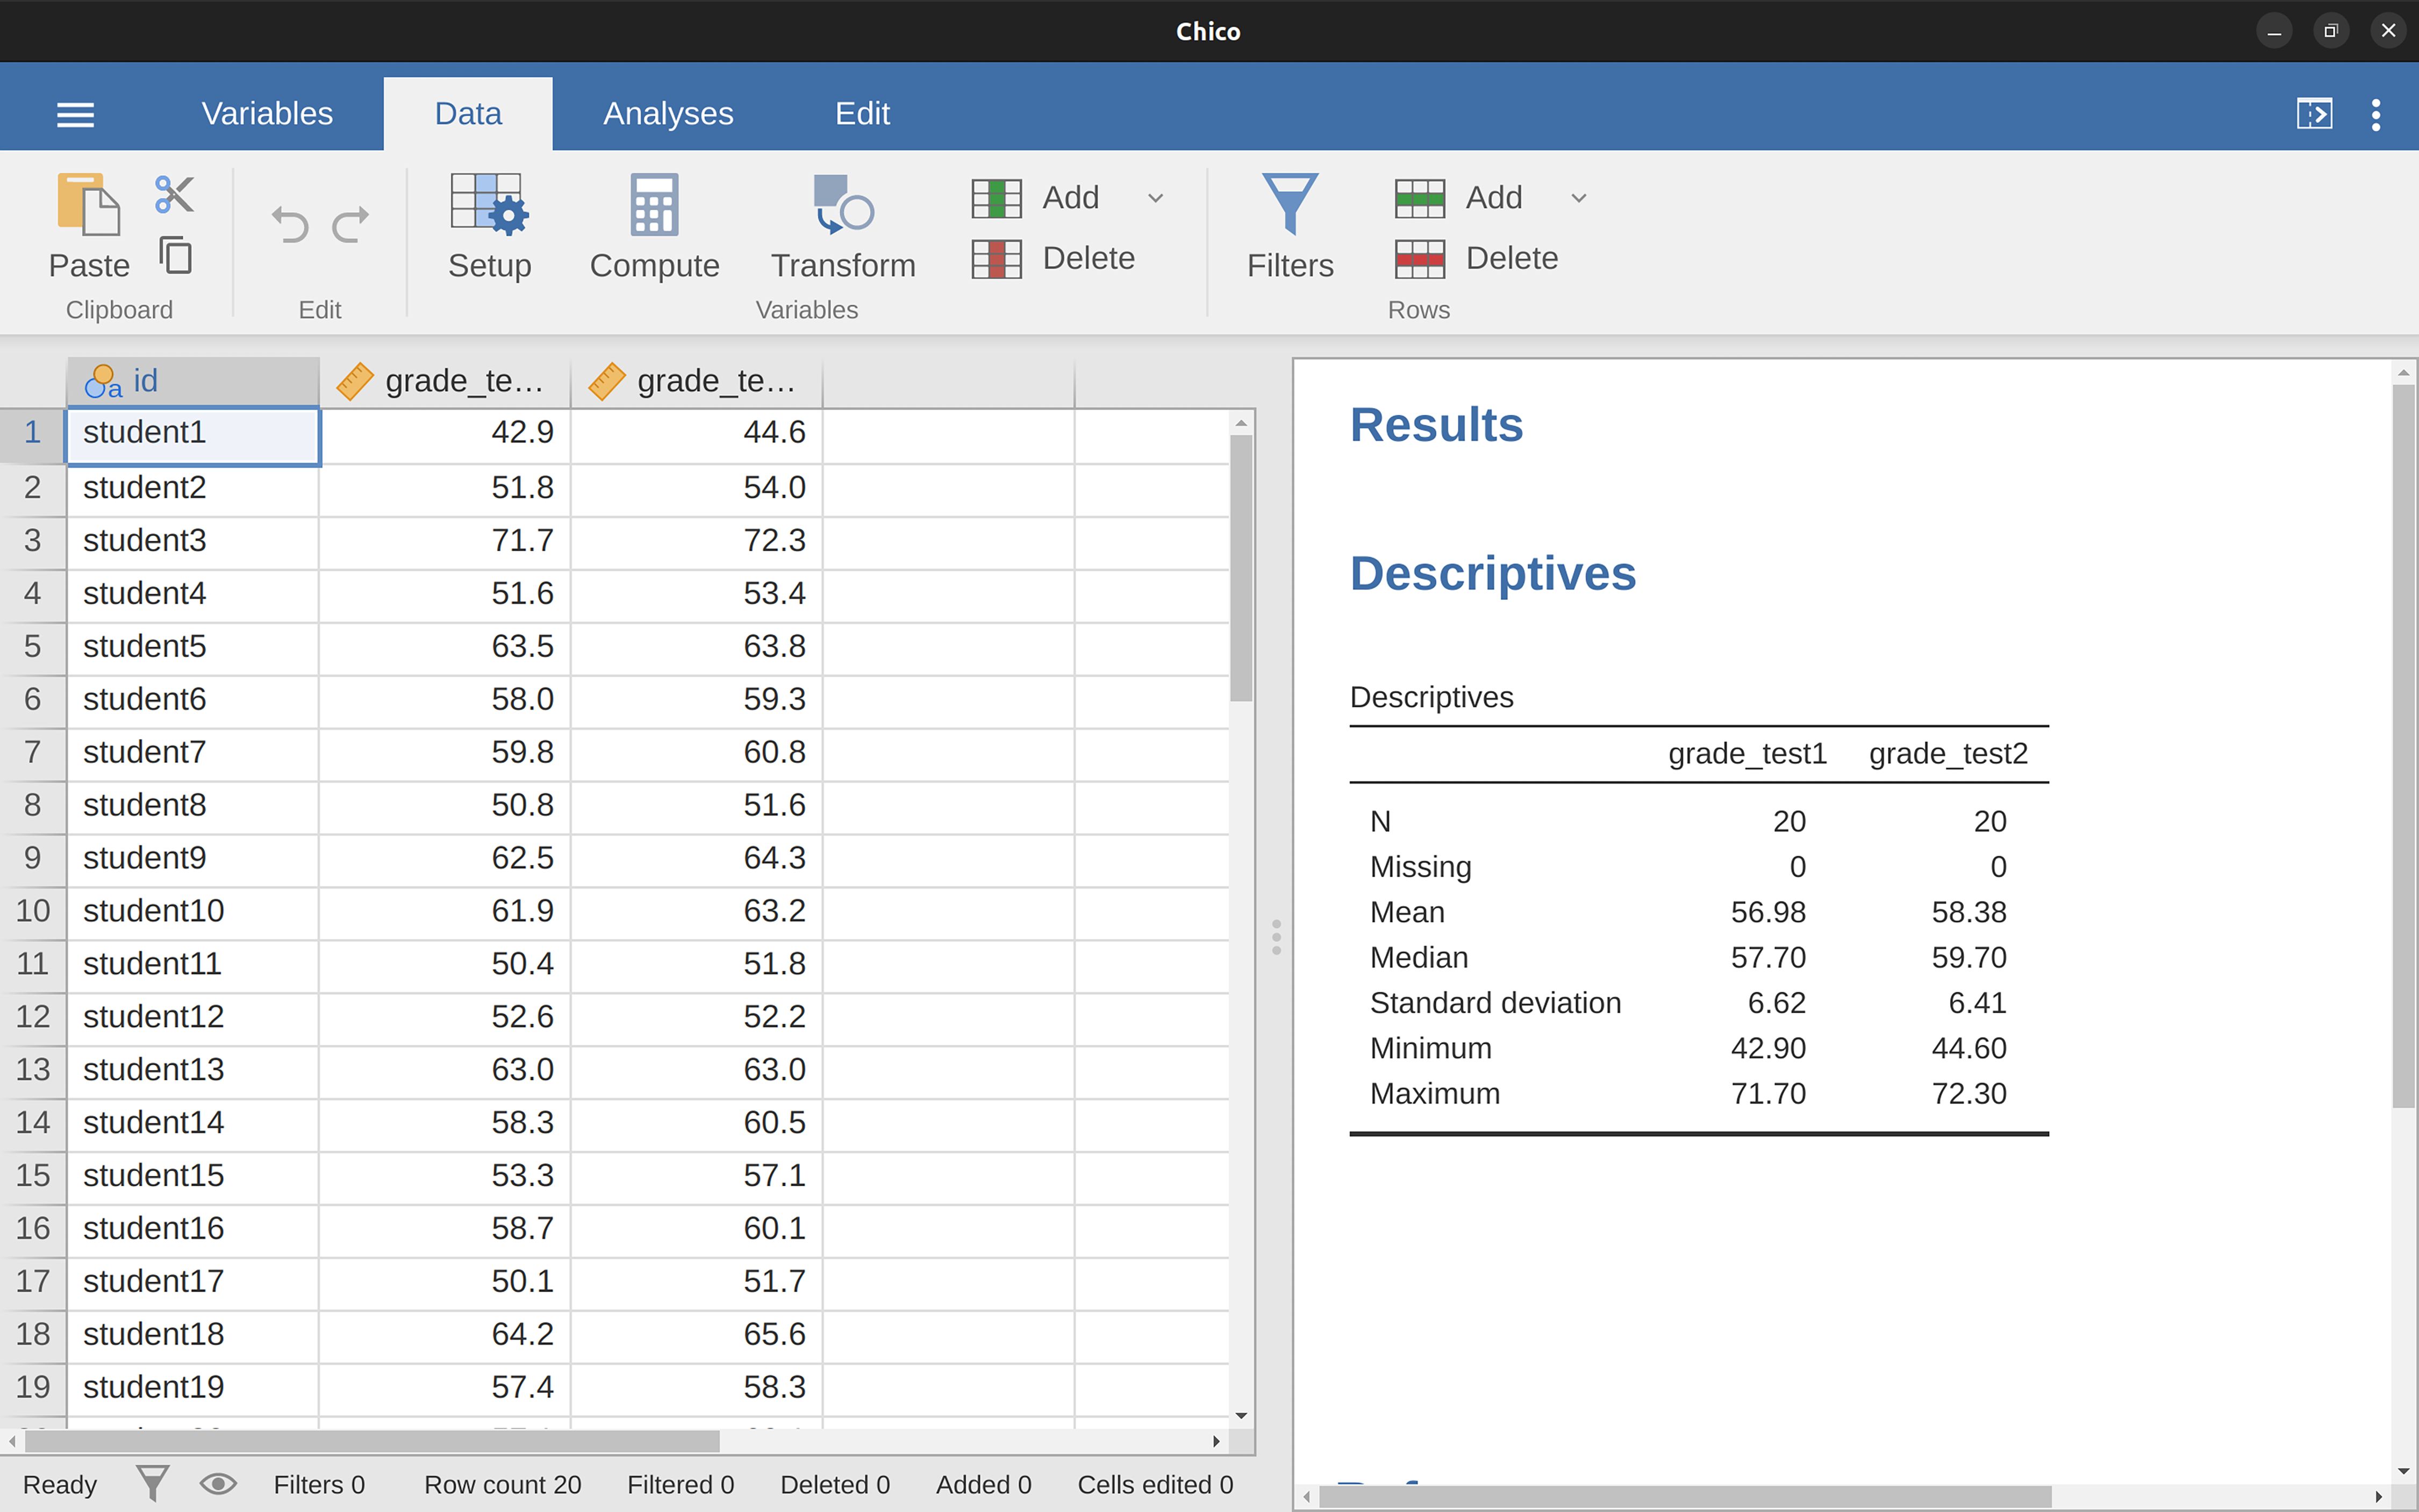
\includegraphics[width=1\textwidth,height=\textheight]{images/fig11-12.png} \hfill{}

\caption{\label{fig-fig16-2}Independent samples \(t\)-test result in
jamovi}

\end{figure}

What does the Bayesian version of the \(t\)-test look like? We can get
the Bayes factor analysis by selecting the `Bayes factor' checkbox under
the `Tests' option, and accepting the suggested default value for the
`Prior'. This gives the results shown in the table in
Figure~\ref{fig-fig16-3}. What we get in this table is a Bayes factor
statistic of 1.75, meaning that the evidence provided by these data are
about 1.8:1 in favour of the alternative hypothesis.

Before moving on, it's worth highlighting the difference between the
orthodox test results and the Bayesian one. According to the orthodox
test, we obtained a significant result, though only barely.
Nevertheless, many people would happily accept \(p = .043\) as
reasonably strong evidence for an effect. In contrast, notice that the
Bayesian test doesn't even reach 2:1 odds in favour of an effect, and
would be considered very weak evidence at best. In my experience that's
a pretty typical outcome. Bayesian methods usually require more evidence
before rejecting the null.

\begin{figure}

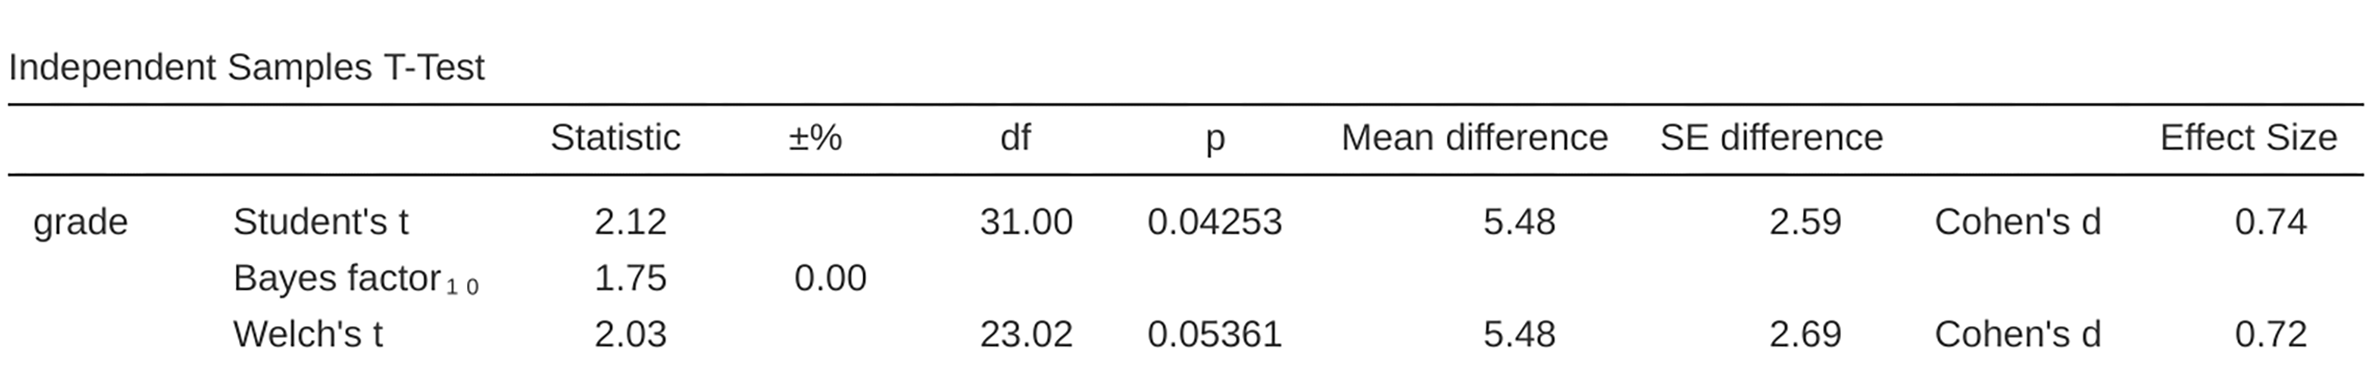
\includegraphics[width=1\textwidth,height=\textheight]{images/fig16-3.png} \hfill{}

\caption{\label{fig-fig16-3}Bayes factors analysis alongside independent
samples \(t\)-test}

\end{figure}

\hypertarget{paired-samples-t-test}{%
\subsection{\texorpdfstring{Paired samples
\(t\)-test}{Paired samples t-test}}\label{paired-samples-t-test}}

Back in Section 11.5 I discussed the \emph{chico.csv} data set in which
student grades were measured on two tests, and we were interested in
finding out whether grades went up from test 1 to test 2. Because every
student did both tests, the tool we used to analyse the data was a
paired samples \(t\)-test. Figure~\ref{fig-fig16-4} shows the jamovi
results table for the conventional paired \(t\)-test alongside the Bayes
factor analysis. At this point, I hope you can read this output without
any difficulty. The data provide evidence of about 6000:1 in favour of
the alternative. We could probably reject the null with some confidence!

\begin{figure}

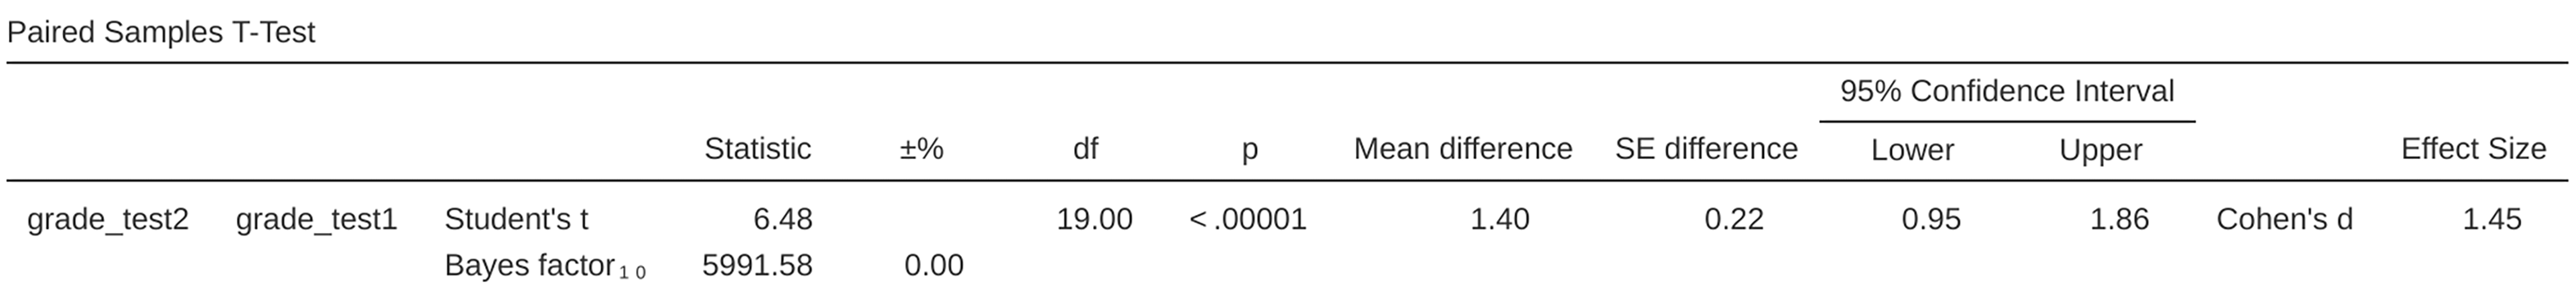
\includegraphics[width=1\textwidth,height=\textheight]{images/fig16-4.png} \hfill{}

\caption{\label{fig-fig16-4}Paired samples \(t\)-test and Bayes factor
result in jamovi}

\end{figure}

\hypertarget{summary-1}{%
\section{Summary}\label{summary-1}}

The first half of this chapter was focused primarily on the theoretical
underpinnings of Bayesian statistics. I introduced the mathematics for
how Bayesian inference works in the section on
\protect\hyperlink{probabilistic-reasoning-by-rational-agents}{Probabilistic
reasoning by rational agents}, and gave a very basic overview of
Bayesian hypothesis tests{]}. Finally, I devoted some space to talking
about why I think \href{Why\%20be\%20a\%20Bayesian?}{Bayesian methods
are worth using}.

Then I gave a practical example, with
\protect\hyperlink{bayesian-t-tests}{Bayesian \(t\)-tests}. If you're
interested in learning more about the Bayesian approach, there are many
good books you could look into. John Kruschke's book, \emph{Doing
Bayesian Data Analysis}, is a pretty good place to start (Kruschke,
2011) and is a nice mix of theory and practice. His approach is a little
different to the ``Bayes factor'' approach that I've discussed here, so
you won't be covering the same ground. If you're a cognitive
psychologist, you might want to check out Lee \& Wagenmakers (2014). I
picked these two because I think they're especially useful for people in
my discipline, but there's a lot of good books out there, so look
around!

\bookmarksetup{startatroot}

\hypertarget{epilogue}{%
\chapter*{Epilogue}\label{epilogue}}
\addcontentsline{toc}{chapter}{Epilogue}

\markboth{Epilogue}{Epilogue}

\placetextbox{0.26}{0.06}{\scriptsize{©2025 D. Foxcroft and D. Navarro,}}
\placetextbox{0.20}{0.05}{\scriptsize{CC BY-NC 4.0}}
\placetextbox{0.70}{0.06}{\scriptsize{\url{https://doi.org/10.11647/OBP.0333/17}}}

\begin{quote}
\emph{``Begin at the beginning'', the King said, very gravely, ``and go
on till you come to the end: then stop''} -- Lewis Carroll, \emph{Alice
in Wonderland}
\end{quote}

\hypertarget{the-undiscovered-statistics}{%
\section*{The undiscovered
statistics}\label{the-undiscovered-statistics}}
\addcontentsline{toc}{section}{The undiscovered statistics}

\markright{The undiscovered statistics}

First, I'm going to talk a bit about some of the content that I wish I'd
had the chance to cram into this book, just so that you can get a sense
of what other ideas are out there in the world of statistics. One thing
that students often fail to realise is that their introductory
statistics classes are just that, an introduction. If you want to go out
into the wider world and do real data analysis, you have to learn a
whole lot of new tools that extend the content of your undergraduate
lectures in all sorts of different ways. Don't assume that something
can't be done just because it wasn't covered in undergrad. Don't assume
that something is the right thing to do just because it was covered in
an undergrad class. To stop you from falling victim to that trap, I
think it's useful to give a bit of an overview of some of the other
ideas out there.

\hypertarget{omissions-within-the-topics-covered}{%
\subsection*{Omissions within the topics
covered}\label{omissions-within-the-topics-covered}}
\addcontentsline{toc}{subsection}{Omissions within the topics covered}

Even within the topics that I have covered in the book, there are a lot
of omissions that I'd like to redress in the future version. Just
sticking to things that are purely about statistics (rather than things
associated with jamovi), the following is a representative but not
exhaustive list of topics that I'd like to expand on at some time:

\begin{itemize}
\item
  \textbf{Other types of correlations.} In
  \textbf{?@sec-Correlation-and-linear-regression} I talked about two
  types of correlation: Pearson and Spearman. Both of these methods of
  assessing correlation are applicable to the case where you have two
  continuous variables and want to assess the relationship between them.
  What about the case where your variables are both nominal scale? Or
  when one is nominal scale and the other is continuous? There are
  actually methods for computing correlations in such cases (e.g.,
  polychoric correlation), and it would be good to see these included.
\item
  \textbf{More detail on effect sizes.} In general, I think the
  treatment of effect sizes throughout the book is a little more cursory
  than it should be. In almost every instance, I've tended just to pick
  one measure of effect size (usually the most popular one) and describe
  that. However, for almost all tests and models there are multiple ways
  of thinking about effect size, and I'd like to go into more detail in
  the future.
\item
  \textbf{Dealing with violated assumptions.} In a number of places in
  the book I've talked about some things you can do when you find that
  the assumptions of your test (or model) are violated, but I think that
  I ought to say more about this. In particular, I think it would have
  been nice to talk in a lot more detail about how you can tranform
  variables to fix problems. I talked a bit about this in
  \textbf{?@sec-Pragmatic-matters}, but the discussion isn't detailed
  enough I think.
\item
  \textbf{Interaction terms for regression.} In
  \textbf{?@sec-Factorial-ANOVA} I talked about the fact that you can
  have interaction terms in an ANOVA, and I also pointed out that ANOVA
  can be interpreted as a kind of linear regression model. Yet, when
  talking about regression in
  \textbf{?@sec-Correlation-and-linear-regression} I made no mention of
  interactions at all. However, there's nothing stopping you from
  including interaction terms in a regression model. It's just a little
  more complicated to figure out what an ``interaction'' actually means
  when you're talking about the interaction between two continuous
  predictors, and it can be done in more than one way. Even so, I would
  have liked to talk a little about this.
\item
  \textbf{Method of planned comparison.} As I mentioned this in
  \textbf{?@sec-Factorial-ANOVA}, it's not always appropriate to be
  using a post hoc correction like Tukey's HSD when doing an ANOVA,
  especially when you had a very clear (and limited) set of comparisons
  that you cared about ahead of time. I would like to talk more about
  this in the future.
\item
  \textbf{Multiple comparison methods.} Even within the context of
  talking about post hoc tests and multiple comparisons, I would have
  liked to talk about the methods in more detail, and talk about what
  other methods exist besides the few options I mentioned.
\end{itemize}

\hypertarget{statistical-models-missing-from-the-book}{%
\subsection*{Statistical models missing from the
book}\label{statistical-models-missing-from-the-book}}
\addcontentsline{toc}{subsection}{Statistical models missing from the
book}

Statistics is a huge field. The core tools that I've described in this
book (chi-square tests, \(t\)-tests, regression and ANOVA) are basic
tools that are widely used in everyday data analysis, and they form the
core of most introductory stats books. However, there are a lot of other
tools out there. There are so very many data analysis situations that
these tools don't cover, and it would be great to give you a sense of
just how much more there is, for example:

\begin{itemize}
\item
  \textbf{Nonlinear regression.} When discussing regression in
  \textbf{?@sec-Correlation-and-linear-regression}, we saw that
  regression assumes that the relationship between predictors and
  outcomes is linear. On the other hand, when we talked about the
  simpler problem of correlation in
  \textbf{?@sec-Descriptive-statistics}, we saw that there exist tools
  (e.g., Spearman correlations) that are able to assess non-linear
  relationships between variables. There are a number of tools in
  statistics that can be used to do non-linear regression. For instance,
  some non-linear regression models assume that the relationship between
  predictors and outcomes is monotonic (e.g., isotonic regression),
  while others assume that it is smooth but not necessarily monotonic
  (e.g., Lowess regression), while others assume that the relationship
  is of a known form that happens to be nonlinear (e.g., polynomial
  regression).
\item
  \textbf{Logistic regression.} Yet another variation on regression
  occurs when the outcome variable is binary, but the predictors are
  continuous. For instance, suppose you're investigating social media,
  and you want to know if it's possible to predict whether or not
  someone is on Twitter as a function of their income, their age, and a
  range of other variables. This is basically a regression model, but
  you can't use regular linear regression because the outcome variable
  is binary (you're either on Twitter or you're not). Because the
  outcome variable is binary, there's no way that the residuals could
  possibly be normally distributed. There are a number of tools that
  statisticians can apply to this situation, the most prominent of which
  is logistic regression.
\item
  \textbf{The General Linear Model (GLM).} The GLM is actually a family
  of models that includes logistic regression, linear regression, (some)
  nonlinear regression, ANOVA and many others. The basic idea in the GLM
  is essentially the same idea that underpins linear models, but it
  allows for the idea that your data might not be normally distributed,
  and allows for nonlinear relationships between predictors and
  outcomes. There are a lot of very handy analyses that you can run that
  fall within the GLM, so it's a very useful thing to know about.
\item
  \textbf{Survival analysis.} In
  \textbf{?@sec-A-brief-introduction-to-research-design} I talked about
  ``differential attrition'', the tendency for people to leave the study
  in a non-random fashion. Back then, I was talking about it as a
  potential methodological concern, but there are a lot of situations in
  which differential attrition is actually the thing you're interested
  in. Suppose, for instance, you're interested in finding out how long
  people play different kinds of computer games in a single session. Do
  people tend to play RTS (real time strategy) games for longer
  stretches than FPS (first person shooter) games? You might design your
  study like this. People come into the lab, and they can play for as
  long or as little as they like. Once they're finished, you record the
  time they spent playing. However, due to ethical restrictions, let's
  suppose that you cannot allow them to keep playing longer than two
  hours. A lot of people will stop playing before the two-hour limit, so
  you know exactly how long they played. But some people will run into
  the two-hour limit, and so you don't know how long they would have
  kept playing if you'd been able to continue the study. As a
  consequence, your data are systematically censored: you're missing all
  of the very long times. How do you analyse this data sensibly? This is
  the problem that survival analysis solves. It is specifically designed
  to handle this situation, where you're systematically missing one
  ``side'' of the data because the study ended. It's very widely used in
  health research, and in that context it is often literally used to
  analyse survival. For instance, you may be tracking people with a
  particular type of cancer, some who have received treatment A and
  others who have received treatment B, but you only have funding to
  track them for five years. At the end of the study period some people
  are alive, others are not. In this context, survival analysis is
  useful for determining which treatment is more effective, and telling
  you about the risk of death that people face over time.
\item
  \textbf{Mixed models.} Repeated measures ANOVA is often used in
  situations where you have observations clustered within experimental
  units. A good example of this is when you track individual people
  across multiple time points. Let's say you're tracking happiness over
  time, for two people. Aaron's happiness starts at 10, then drops to 8,
  and then to 6. Belinda's happiness starts at 6, then rises to 8 and
  then to 10. Both of these two people have the same ``overall'' level
  of happiness (the average across the three time points is 8), so a
  repeated measures ANOVA analysis would treat Aaron and Belinda the
  same way. But that's clearly wrong. Aaron's happiness is decreasing,
  whereas Belinda's is increasing. If you want to optimally analyse data
  from an experiment where people can change over time, then you need a
  more powerful tool than repeated measures ANOVA. The tools that people
  use to solve this problem are called ``mixed'' models, because they
  are designed to learn about individual experimental units (e.g.,
  happiness of individual people over time) as well as overall effects
  (e.g., the effect of money on happiness over time). Repeated measures
  ANOVA is perhaps the simplest example of a mixed model, but there's a
  lot you can do with mixed models that you can't do with repeated
  measures ANOVA.
\item
  \textbf{Multidimensional scaling.} Factor Analysis is an example of an
  ``unsupervised learning'' model. What this means is that, unlike most
  of the ``supervised learning'' tools I've mentioned, you can't divide
  up your variables into predictors and outcomes. Regression is
  supervised learning whereas Factor Analysis is unsupervised learning.
  It's not the only type of unsupervised learning model however. For
  example, in Factor Analysis one is concerned with the analysis of
  correlations between variables. However, there are many situations
  where you're actually interested in analysing similarities or
  dissimilarities between objects, items or people. There are a number
  of tools that you can use in this situation, the best known of which
  is multidimensional scaling (MDS). In MDS, the idea is to find a
  ``geometric'' representation of your items. Each item is ``plotted''
  as a point in some space, and the distance between two points is a
  measure of how dissimilar those items are.
\item
  \textbf{Clustering.} Another example of an unsupervised learning model
  is clustering (also referred to as classification), in which you want
  to organise all of your items into meaningful groups, such that
  similar items are assigned to the same groups. A lot of clustering is
  unsupervised, meaning that you don't know anything about what the
  groups are, you just have to guess. There are other ``supervised
  clustering'' situations where you need to predict group memberships on
  the basis of other variables, and those group memberships are actually
  observables. Logistic regression is a good example of a tool that
  works this way. However, when you don't actually know the group
  memberships, you have to use different tools (e.g., k-means
  clustering). There are even situations where you want to do something
  called ``semi-supervised clustering'', in which you know the group
  memberships for some items but not others. As you can probably guess,
  clustering is a pretty big topic, and a pretty useful thing to know
  about.
\item
  \textbf{Causal models.} One thing that I haven't talked about much in
  this book is how you can use statistical modelling to learn about the
  causal relationships between variables. For instance, consider the
  following three variables which might be of interest when thinking
  about how someone died in a firing squad. We might want to measure
  whether or not an execution order was given (variable A), whether or
  not a marksman fired their gun (variable B), and whether or not the
  person got hit with a bullet (variable C). These three variables are
  all correlated with one another (e.g., there is a correlation between
  guns being fired and people getting hit with bullets), but we actually
  want to make stronger statements about them than merely talking about
  correlations. We want to talk about causation. We want to be able to
  say that the execution order (A) causes the marksman to fire (B) which
  causes someone to get shot (C). We can express this by a directed
  arrow notation: we write it as \(A \rightarrow B \rightarrow C\). This
  ``causal chain'' is a fundamentally different explanation for events
  than one in which the marksman fires first, which causes the shooting
  \(B \rightarrow C\), and then causes the executioner to
  ``retroactively'' issue the execution order, \(B \rightarrow A\). This
  ``common effect'' model says that A and C are both caused by B. You
  can see why these are different. In the first causal model, if we had
  managed to stop the executioner from issuing the order (intervening to
  change A), then no shooting would have happened. In the second model,
  the shooting would have happened any way because the marksman was not
  following the execution order. There is a big literature in statistics
  on trying to understand the causal relationships between variables,
  and a number of different tools exist to help you test different
  causal stories about your data. The most widely used of these tools
  (in psychology at least) is structural equations modelling (SEM), and
  at some point I'd like to extend the book to talk about it.
\end{itemize}

Of course, even this listing is incomplete. I haven't mentioned time
series analysis, item response theory, market basket analysis,
classification and regression trees, or any of a huge range of other
topics. However, the list that I've given above is essentially my wish
list for this book. Sure, it would double the length of the book, but it
would mean that the scope has become broad enough to cover most things
that applied researchers in psychology would need to use.

\hypertarget{other-ways-of-doing-inference}{%
\subsection*{Other ways of doing
inference}\label{other-ways-of-doing-inference}}
\addcontentsline{toc}{subsection}{Other ways of doing inference}

A different sense in which this book is incomplete is that it focuses
pretty heavily on a very narrow and old-fashioned view of how
inferential statistics should be done. In
\textbf{?@sec-Estimating-unknown-quantities-from-a-sample} I talked a
little bit about the idea of unbiased estimators, sampling distributions
and so on. In \textbf{?@sec-Hypothesis-testing} I talked about the
theory of null hypothesis significance testing and \(p\)-values. These
ideas have been around since the early 20th century, and the tools that
I've talked about in the book rely very heavily on the theoretical ideas
from that time. I've felt obligated to stick to those topics because the
vast majority of data analysis in science is also reliant on those
ideas. However, the theory of statistics is not restricted to those
topics and, whilst everyone should know about them because of their
practical importance, in many respects those ideas do not represent best
practice for contemporary data analysis. One of the things that I'm
especially happy with is that I've been able to go a little beyond this.
Chapter~\ref{sec-Bayesian-statistics} now presents the Bayesian
perspective in a reasonable amount of detail, but the book overall is
still pretty heavily weighted towards the frequentist orthodoxy.
Additionally, there are a number of other approaches to inference that
are worth mentioning:

\begin{itemize}
\item
  Bootstrapping. Throughout the book, whenever I've introduced a
  hypothesis test, I've had a strong tendency just to make assertions
  like ``the sampling distribution for BLAH is a \(t\)-distribution'' or
  something like that. In some cases, I've actually attempted to justify
  this assertion. For example, when talking about \(\chi^2\) tests in
  \textbf{?@sec-Categorical-data-analysis} I made reference to the known
  relationship between normal distributions and \(\chi^2\) distributions
  (see \textbf{?@sec-Introduction-to-probability}) to explain how we end
  up assuming that the sampling distribution of the goodness-of-fit
  statistic is \(\chi^2\). However, it's also the case that a lot of
  these sampling distributions are, well, wrong. The \(\chi^2\) test is
  a good example. It is based on an assumption about the distribution of
  your data, an assumption which is known to be wrong for small sample
  sizes! Back in the early 20th century, there wasn't much you could do
  about this situation. Statisticians had developed mathematical results
  that said that ``under assumptions BLAH about the data, the sampling
  distribution is approximately BLAH'', and that was about the best you
  could do. A lot of times they didn't even have that. There are lots of
  data analysis situations for which no-one has found a mathematical
  solution for the sampling distributions that you need. And so up until
  the late 20th century, the corresponding tests didn't exist or didn't
  work. However, computers have changed all that now. There are lots of
  fancy tricks, and some not-so-fancy, that you can use to get around
  it. The simplest of these is bootstrapping, and in it's simplest form
  it's incredibly simple. What you do is simulate the results of your
  experiment lots and lots of times, under the twin assumptions that (a)
  the null hypothesis is true and (b) the unknown population
  distribution actually looks pretty similar to your raw data. In other
  words, instead of assuming that the data are (for instance) normally
  distributed, just assume that the population looks the same as your
  sample, and then use computers to simulate the sampling distribution
  for your test statistic if that assumption holds. Despite relying on a
  somewhat dubious assumption (i.e., the population distribution is the
  same as the sample!) bootstrapping is quick and easy method that works
  remarkably well in practice for lots of data analysis problems.
\item
  Cross validation. One question that pops up in my stats classes every
  now and then, usually by a student trying to be provocative, is ``Why
  do we care about inferential statistics at all? Why not just describe
  your sample?'' The answer to the question is usually something like
  this, ``Because our true interest as scientists is not the specific
  sample that we have observed in the \emph{past}, we want to make
  predictions about data we might observe in the future''. A lot of the
  issues in statistical inference arise because of the fact that we
  always expect the future to be similar to but a bit different from the
  past. Or, more generally, new data won't be quite the same as old
  data. What we do, in a lot of situations, is try to derive
  mathematical rules that help us to draw the inferences that are most
  likely to be correct for new data, rather than to pick the statements
  that best describe old data. For instance, given two models A and B,
  and a data set \(X\) you collected today, try to pick the model that
  will best describe a new data set \(Y\) that you're going to collect
  tomorrow. Sometimes it's convenient to simulate the process, and
  that's what cross-validation does. What you do is divide your data set
  into two subsets, \(X_1\) and \(X_2\). Use the subset \(X_1\) to train
  the model (e.g., estimate regression coefficients, let's say), but
  then assess the model performance on the other one \(X_2\). This gives
  you a measure of how well the model generalises from an old data set
  to a new one, and is often a better measure of how good your model is
  than if you just fit it to the full data set \(X\).
\item
  Robust statistics. Life is messy, and nothing really works the way
  it's supposed to. This is just as true for statistics as it is for
  anything else, and when trying to analyse data we're often stuck with
  all sorts of problems in which the data are just messier than they're
  supposed to be. Variables that are supposed to be normally distributed
  are not actually normally distributed, relationships that are supposed
  to be linear are not actually linear, and some of the observations in
  your data set are almost certainly junk (i.e., not measuring what
  they're supposed to). All of this messiness is ignored in most of the
  statistical theory I developed in this book. However, ignoring a
  problem doesn't always solve it. Sometimes, it's actually okay to
  ignore the mess, because some types of statistical tools are
  ``robust'', i.e., if the data don't satisfy your theoretical
  assumptions they nevertheless still work pretty well. Other types of
  statistical tools are not robust, and even minor deviations from the
  theoretical assumptions cause them to break. Robust statistics is a
  branch of stats concerned with this question, and they talk about
  things like the ``breakdown point'' of a statistic. That is, how messy
  does your data have to be before the statistic cannot be trusted? I
  touched on this in places. The mean is not a robust estimator of the
  central tendency of a variable, but the median is. For instance,
  suppose I told you that the ages of my five best friends are 34, 39,
  31, 43 and 4003 years. How old do you think they are on average? That
  is, what is the true population mean here? If you use the sample mean
  as your estimator of the population mean, you get an answer of 830
  years. If you use the sample median as the estimator of the population
  mean, you get an answer of 39 years. Notice that, even though you're
  ``technically'' doing the wrong thing in the second case (using the
  median to estimate the mean!) you're actually getting a better answer.
  The problem here is that one of the observations is clearly,
  obviously, a lie. I don't have a friend aged 4003 years. It's probably
  a typo, I probably meant to type 43. But what if I had typed 53
  instead of 43, or 34 instead of 43? Could you be sure if this was a
  typo or not? Sometimes the errors in the data are subtle, so you can't
  detect them just by eyeballing the sample, but they're still errors
  that contaminate your data, and they still affect your conclusions.
  Robust statistics is concerned with how you can make safe inferences
  even when faced with contamination that you don't know about. It's
  pretty cool stuff.
\end{itemize}

\hypertarget{miscellaneous-topics}{%
\subsection*{Miscellaneous topics}\label{miscellaneous-topics}}
\addcontentsline{toc}{subsection}{Miscellaneous topics}

\begin{itemize}
\item
  Suppose you're doing a survey, and you're interested in exercise and
  weight. You send data to four people. Adam says he exercises a lot and
  is not overweight. Briony says she exercises a lot and is not
  overweight. Carol says she does not exercise and is overweight. Tim
  says he does not exercise and refuses to answer the question about his
  weight. Elaine does not return the survey. You now have a missing data
  problem. There is one entire survey missing, and one question missing
  from another one, What do you do about it? Ignoring missing data is
  not, in general, a safe thing to do. Let's think about Tim's survey
  here. Firstly, notice that, on the basis of his other responses, he
  appear to be more similar to Carol (neither of us exercise) than to
  Adam or Briony. So if you were forced to guess his weight, you'd guess
  that he is closer to her than to them. Maybe you'd make some
  correction for the fact that Adam and Tim are males and Briony and
  Carol are females. The statistical name for this kind of guessing is
  ``imputation''. Doing imputation safely is hard, but it's important,
  especially when the missing data are missing in a systematic way.
  Because of the fact that people who are overweight are often pressured
  to feel poorly about their weight (often thanks to public health
  campaigns), we actually have reason to suspect that the people who are
  not responding are more likely to be overweight than the people who do
  respond. Imputing a weight to Tim means that the number of overweight
  people in the sample will probably rise from 1 out of 3 (if we ignore
  Tim), to 2 out of 4 (if we impute Tim's weight). Clearly this matters.
  But doing it sensibly is more complicated than it sounds. Earlier, I
  suggested you should treat Tim like Carol, since they gave the same
  answer to the exercise question. But that's not quite right. There is
  a systematic difference between them. She answered the question, and
  Tim didn't. Given the social pressures faced by overweight people,
  isn't it likely that Tim is \emph{more} overweight than Carol? And of
  course this is still ignoring the fact that it's not sensible to
  impute a \emph{single} weight to Tim, as if you actually knew his
  weight. Instead, what you need to do it is impute a range of plausible
  guesses (referred to as multiple imputation), in order to capture the
  fact that you're more uncertain about Tim's weight than you are about
  Carol's. And let's not get started on the problem posed by the fact
  that Elaine didn't send in the survey. As you can probably guess,
  dealing with missing data is an increasingly important topic. In fact,
  I've been told that a lot of journals in some fields will not accept
  studies that have missing data unless some kind of sensible multiple
  imputation scheme is followed.
\item
  Power analysis. In \textbf{?@sec-Hypothesis-testing} I discussed the
  concept of power (i.e., how likely are you to be able to detect an
  effect if it actually exists) and referred to power analysis, a
  collection of tools that are useful for assessing how much power your
  study has. Power analysis can be useful for planning a study (e.g.,
  figuring out how large a sample you're likely to need), but it also
  serves a useful role in analysing data that you already collected. For
  instance, suppose you get a significant result, and you have an
  estimate of your effect size. You can use this information to estimate
  how much power your study actually had. This is kind of useful,
  especially if your effect size is not large. For instance, suppose you
  reject the null hypothesis at \(p< .05\), but you use power analysis
  to figure out that your estimated power was only .08. The significant
  result means that, if the null hypothesis was in fact true, there was
  a 5\% chance of getting data like this. But the low power means that,
  even if the null hypothesis is false and the effect size was really as
  small as it looks, there was only an 8\% chance of getting data like
  you did. This suggests that you need to be pretty cautious, because
  luck seems to have played a big part in your results, one way or the
  other!
\item
  Data analysis using theory-inspired models. In a few places in this
  book I've mentioned response time (RT) data, where you record how long
  it takes someone to do something (e.g., make a simple decision). I've
  mentioned that RT data are almost invariably non-normal, and
  positively skewed. Additionally, there's a thing known as the speed /
  accuracy trade-off: if you try to make decisions too quickly (low RT)
  then you're likely to make poorer decisions (lower accuracy). So if
  you measure both the accuracy of a participant's decisions and their
  RT, you'll probably find that speed and accuracy are related. There's
  more to the story than this, of course, because some people make
  better decisions than others regardless of how fast they're going.
  Moreover, speed depends on both cognitive processes (i.e., time spent
  thinking) but also physiological ones (e.g., how fast can you move
  your muscles). It's starting to sound like analysing this data will be
  a complicated process. And indeed it is, but one of the things that
  you find when you dig into the psychological literature is that there
  already exist mathematical models (called ``sequential sampling
  models'') that describe how people make simple decisions, and these
  models take into account a lot of the factors I mentioned above. You
  won't find any of these theoretically-inspired models in a standard
  statistics textbook. Standard stats textbooks describe standard tools,
  tools that could meaningfully be applied in lots of different
  disciplines, not just psychology. ANOVA is an example of a standard
  tool that is just as applicable to psychology as to pharmacology.
  Sequential sampling models are not, they are psychology-specific, more
  or less. This doesn't make them less powerful tools. In fact, if
  you're analysing data where people have to make choices quickly you
  should really be using sequential sampling models to analyse the data.
  Using ANOVA or regression or whatever won't work as well, because the
  theoretical assumptions that underpin them are not well-matched to
  your data. In contrast, sequential sampling models were explicitly
  designed to analyse this specific type of data, and their theoretical
  assumptions are extremely well-matched to the data.
\end{itemize}

\hypertarget{learning-the-basics-and-learning-them-in-jamovi}{%
\section*{Learning the basics, and learning them in
jamovi}\label{learning-the-basics-and-learning-them-in-jamovi}}
\addcontentsline{toc}{section}{Learning the basics, and learning them in
jamovi}

\markright{Learning the basics, and learning them in jamovi}

Okay, that was a long list. And even that listing is massively
incomplete. There really are a lot of big ideas in statistics that I
haven't covered in this book. It can seem pretty depressing to finish an
almost 500-page textbook only to be told that this is only the
beginning, especially when you start to suspect that half of the stuff
you've been taught is wrong. For instance, there are a lot of people in
the field who would strongly argue against the use of the classical
ANOVA model, yet I've devoted two whole chapters to it! Standard ANOVA
can be attacked from a Bayesian perspective, or from a robust statistics
perspective, or even from a ``it's just plain wrong'' perspective
(people very frequently use ANOVA when they should actually be using
mixed models). So why learn it at all?

As I see it, there are two key arguments. Firstly, there's the pure
pragmatism argument. Rightly or wrongly, ANOVA is widely used. If you
want to understand the scientific literature, you need to understand
ANOVA. And secondly, there's the ``incremental knowledge'' argument. In
the same way that it was handy to have seen one-way ANOVA before trying
to learn factorial ANOVA, understanding ANOVA is helpful for
understanding more advanced tools, because a lot of those tools extend
on or modify the basic ANOVA setup in some way. For instance, although
mixed models are way more useful than ANOVA and regression, I've never
heard of anyone learning how mixed models work without first having
worked through ANOVA and regression. You have to learn to crawl before
you can climb a mountain.

Actually, I want to push this point a bit further. One thing that I've
done a lot of in this book is talk about fundamentals. I spent a lot of
time on probability theory. I talked about the theory of estimation and
hypothesis tests in more detail than I needed to. Why did I do all this?
Looking back, you might ask whether I really needed to spend all that
time talking about what a probability distribution is, or why there was
even a section on probability density. If the goal of the book was to
teach you how to run a \(t\)-test or an ANOVA, was all that really
necessary? Was this all just a huge waste of everyone's time???

The answer, I hope you'll agree, is no. The goal of an introductory
stats is not to teach ANOVA. It's not to teach \(t\)-tests, or
regressions, or histograms, or \(p\)-values. The goal is to start you on
the path towards becoming a skilled data analyst. And in order for you
to become a skilled data analyst, you need to be able to do more than
ANOVA, more than \(t\)-tests, regressions and histograms. You need to be
able to think properly about data. You need to be able to learn the more
advanced statistical models that I talked about in the last section, and
to understand the theory upon which they are based. And you need to have
access to software that will let you use those advanced tools. And this
is where, in my opinion at least, all that extra time I've spent on the
fundamentals pays off. If you understand probability theory, you'll find
it much easier to switch from frequentist analyses to Bayesian ones.

In short, I think that the big payoff for learning statistics this way
is extensibility. For a book that only covers the very basics of data
analysis, this book has a massive overhead in terms of learning
probability theory and so on. There's a whole lot of other things that
it pushes you to learn besides the specific analyses that the book
covers. So if your goal had been to learn how to run an ANOVA in the
minimum possible time, well, this book wasn't a good choice. But as I
say, I don't think that is your goal. I think you want to learn how to
do data analysis. And if that really is your goal, you want to make sure
that the skills you learn in your introductory stats class are naturally
and cleanly extensible to the more complicated models that you need in
real world data analysis. You want to make sure that you learn to use
the same tools that real data analysts use, so that you can learn to do
what they do. And so yeah, okay, you're a beginner right now (or you
were when you started this book), but that doesn't mean you should be
given a dumbed-down story, a story in which I don't tell you about
probability density, or a story where I don't tell you about the
nightmare that is factorial ANOVA with unbalanced designs. And it
doesn't mean that you should be given baby toys instead of proper data
analysis tools. Beginners aren't dumb, they just lack knowledge. What
you need is not to have the complexities of real-world data analysis
hidden from from you. What you need are the skills and tools that will
let you handle those complexities when they inevitably ambush you in the
real world.

And what I hope is that this book is able to help you with that.

Author's note -- If you see anything clever sounding in this book that
doesn't seem to have a reference, I can absolutely promise you that the
idea was someone else's. This is an introductory textbook: none of the
ideas are original. I'll take responsibility for all the errors, but I
can't take credit for any of the good stuff. Everything smart in this
book came from someone else.

\bookmarksetup{startatroot}

\hypertarget{references}{%
\chapter*{References}\label{references}}
\addcontentsline{toc}{chapter}{References}

\markboth{References}{References}

\hypertarget{refs}{}
\begin{CSLReferences}{1}{0}
\leavevmode\vadjust pre{\hypertarget{ref-Box1953}{}}%
Box, G. E. P. (1953). Non-normality and tests on variances.
\emph{Biometrika}, \emph{40}, 318--335.
\url{https://doi.org/10.2307/2333350}

\leavevmode\vadjust pre{\hypertarget{ref-BrownForsythe1974}{}}%
Brown, M. B., \& Forsythe, A. B. (1974). Robust tests for equality of
variances. \emph{Journal of the American Statistical Association},
\emph{69}, 364--367. \url{https://doi.org/10.2307/2285659}

\leavevmode\vadjust pre{\hypertarget{ref-Dunn1961}{}}%
Dunn, O. J. (1961). Multiple comparisons among means. \emph{Journal of
the American Statistical Association}, \emph{56}, 52--64.
\url{https://doi.org/10.1080/01621459.1961.10482090}

\leavevmode\vadjust pre{\hypertarget{ref-Fisher1925}{}}%
Fisher, R. A. (1925). \emph{Statistical methods for research workers}.
Oliver \& Boyd.

\leavevmode\vadjust pre{\hypertarget{ref-Geschwind1972}{}}%
Geschwind, N. (1972). Language and the brain. \emph{Scientific
American}, \emph{226(4)}, 76--83.
\url{https://doi.org/10.1038/scientificamerican0472-76}

\leavevmode\vadjust pre{\hypertarget{ref-Hays1994}{}}%
Hays, W. L. (1994). \emph{Statistics} (5th ed.). Harcourt Brace.

\leavevmode\vadjust pre{\hypertarget{ref-Holm1979}{}}%
Holm, S. (1979). A simple sequentially rejective multiple test
procedure. \emph{Scandinavian Journal of Statistics}, \emph{6}, 65--70.
\url{https://doi.org/10.2307/4615733}

\leavevmode\vadjust pre{\hypertarget{ref-Hsu1996}{}}%
Hsu, J. C. (1996). \emph{Multiple comparisons: Theory and methods}.
Chapman \& Hall. \url{https://doi.org/10.1201/b15074}

\leavevmode\vadjust pre{\hypertarget{ref-Jeffreys1961}{}}%
Jeffreys, H. (1961). \emph{The theory of probability} (3rd ed.). Oxford.
\url{https://doi.org/10.1093/oso/9780198503682.001.0001}

\leavevmode\vadjust pre{\hypertarget{ref-Johnson2013}{}}%
Johnson, V. E. (2013). Revised standards for statistical evidence.
\emph{Proceedings of the National Academy of Sciences}, \emph{48},
19313--19317. \url{https://doi.org/10.1073/pnas.1313476110}

\leavevmode\vadjust pre{\hypertarget{ref-Kass1995}{}}%
Kass, R. E., \& Raftery, A. E. (1995). Bayes factors. \emph{Journal of
the American Statistical Association}, \emph{90}, 773--795.
\url{https://doi.org/10.1080/01621459.1995.10476572}

\leavevmode\vadjust pre{\hypertarget{ref-Kruschke2011}{}}%
Kruschke, J. K. (2011). \emph{Doing {B}ayesian data analysis: A tutorial
with {R} and {BUGS}}. Academic Press.

\leavevmode\vadjust pre{\hypertarget{ref-KruskalWallis1952}{}}%
Kruskal, W. H., \& Wallis, W. A. (1952). Use of ranks in one-criterion
variance analysis. \emph{Journal of the American Statistical
Association}, \emph{47}, 583--621.
\url{https://doi.org/10.1080/01621459.1952.10483441}

\leavevmode\vadjust pre{\hypertarget{ref-Lee2014}{}}%
Lee, M. D., \& Wagenmakers, E.-J. (2014). \emph{Bayesian cognitive
modeling: A practical course}. Cambridge University Press.
\url{https://doi.org/10.1017/CBO9781139087759}

\leavevmode\vadjust pre{\hypertarget{ref-Levene1960}{}}%
Levene, H. (1960). Robust tests for equality of variances. In Olkin, I.
and others (Ed.), \emph{Contributions to probability and statistics:
Essays in honor of harold hotelling} (pp. 278--292). Stanford University
Press.

\leavevmode\vadjust pre{\hypertarget{ref-Sahai2000}{}}%
Sahai, H., \& Ageel, M. I. (2000). \emph{The analysis of variance:
Fixed, random and mixed models}. Birkhauser.

\leavevmode\vadjust pre{\hypertarget{ref-Shaffer1995}{}}%
Shaffer, J. P. (1995). Multiple hypothesis testing. \emph{Annual Review
of Psychology}, \emph{46}, 561--584.
\url{https://doi.org/10.1146/annurev.ps.46.020195.003021}

\leavevmode\vadjust pre{\hypertarget{ref-Welch1951}{}}%
Welch, B. L. (1951). On the comparison of several mean values: An
alternative approach. \emph{Biometrika}, \emph{38}, 330--336.
\url{https://doi.org/10.1093/biomet/38.3-4.330}

\end{CSLReferences}


\backmatter

\printendnotes
\newpage

\chapter{About the team}

Alessandra Tosi was the managing editor for this book.

Tricia de Souza and Adèle Kreager proof-read this manuscript.

The cover was designed by Jeevanjot Kaur Nagpal, and produced in InDesign using the Fontin and Calibri fonts.

David Foxcroft and Cameron Craig produced the printed PDF editions. 

David Foxcroft produced the HTML edition.

Raegan Allen was in charge of marketing.

This book was peer-reviewed by two referees. Experts in their field, these readers give their time freely to help ensure the academic rigour of our books. We are grateful for their generous and invaluable contributions.

\newpage


%\printindex
%back cover
%\includepdf[fitpaper=true,pages=-]{images/backcover8x10}
%\pagenumbering{gobble} 

\end{document}
